%%%%%%%%%%%%%%%%%%%%%%%%%%%%%%%%%%%%%%%%%%%%%%%%%%%%%%%%%%%%%%%%%%%%%%%%%%%%%%%%
% title:
% authors:
%%%%%%%%%%%%%%%%%%%%%%%%%%%%%%%%%%%%%%%%%%%%%%%%%%%%%%%%%%%%%%%%%%%%%%%%%%%%%%%%
\def\fullver{0}
\def\submission{1}
\documentclass[11pt]{article}

\usepackage[letterpaper,hmargin=1in,vmargin=1in]{geometry}
\usepackage[backref=true,backend=bibtex]{biblatex}

\DefineBibliographyStrings{english}{%
  backrefpage = {page},% originally "cited on page"
  backrefpages = {pages},% originally "cited on pages"
}


\usepackage{framed}
%\usepackage{cite}
\usepackage[hidelinks]{hyperref}

\usepackage{color}
\usepackage{float}
\usepackage{setspace}
\usepackage{booktabs}
\usepackage{outlines}
\usepackage{enumitem}
\usepackage{epsfig}
\usepackage{wrapfig}
\usepackage{textcomp}
\usepackage{rotating}
\usepackage{xspace}
\usepackage{tikz}
\usetikzlibrary{calc,arrows,arrows.meta,shapes,positioning,matrix,decorations.pathreplacing}
\usepackage{amsthm}
\usepackage{amssymb}
\usepackage{pifont}
\usepackage{amsfonts}
\usepackage{amsmath}
\DeclareMathOperator*{\argmax}{arg\,max}
\DeclareMathOperator*{\argmin}{arg\,min}
\usepackage{cleveref}
\usepackage{bm}
\usepackage{listings}
\usepackage{mathtools}
\allowdisplaybreaks[2]
\usepackage{latexsym}
\usepackage{graphics}
\usepackage{graphicx}
\usepackage{fancyhdr}
\usepackage{url}
%\usepackage{enumerate}
\usepackage{adjustbox}
\usepackage{multirow}
\usepackage[font=small]{caption}
\usepackage[font=small]{subcaption}
\def\authnotes{1}
\newtheorem{thm}{} %[section]
\newtheorem*{theorem*}{Theorem}
\newtheorem{lem}{Lemma}

\newtheorem{cor}[thm]{Corollary}
\newtheorem{propo}[thm]{Proposition}
\newtheorem{defn}[thm]{Definition}
\newtheorem{assm}[thm]{Assumption}
\newtheorem{clm}[thm]{Claim}
\newtheorem{rem}[thm]{Remark}
\newtheorem{exa}{Example}
\newtheorem{fact}{Fact}

\newenvironment{theorem}{\begin{thm}
    \begin{sl}
    }%
    {
    \end{sl}
  \end{thm}}

\newenvironment{lemma}{\begin{lem}\begin{sl}}%
    {\end{sl}\end{lem}}
\newenvironment{corollary}{\begin{cor}\begin{sl}}%
    {\end{sl}\end{cor}}
\newenvironment{proposition}{\begin{propo}\begin{sl}}%
    {\end{sl}\end{propo}}
\newenvironment{definition}{\begin{defn}\begin{sl}}%
    {\end{sl}\end{defn}}
\newenvironment{assumption}{\begin{assm}\begin{em}}%
    {\end{em}\end{assm}}
\newenvironment{claim}{\begin{clm}\begin{sl}}%
    {\end{sl}\end{clm}}
\newenvironment{remark}{\begin{rem}\begin{em}}%
    {\end{em}\end{rem}}
\newenvironment{example}{\begin{exa}\begin{em}}%
    {\end{em}\end{exa}}

\newcommand{\lemautorefname}{Lemma}
\newcommand{\algorithmautorefname}{Algorithm}
\renewcommand{\subsectionautorefname}{Section}


% Deluxe proof enviroment
\iffalse
    \def\qsym{\vrule width0.6ex height1em depth0ex}
    \def\qedsym{{\hspace{5pt}\rule[-1pt]{3pt}{9pt}}}
    \newcount\proofqeded
    \newcount\proofended
    \def\qed{%\qedsym
    \end{rm}\addtolength{\parskip}{-0pt}
    \setlength{\parindent}{\saveparindent}
    \global\advance\proofqeded by 1 }
    \newenvironment{proof}%
     {\proofstart}%
     {\ifnum\proofqeded=\proofended\qed\fi \global\advance\proofended by 1
      \medskip}
    \makeatletter
    \def\proofstart{\@ifnextchar[{\@oprf}{\@nprf}}
    \def\@oprf[#1]{\begin{rm}\protect\vspace{6pt}\noindent{\bf Proof of #1:\
    }%
    \addtolength{\parskip}{5pt}\setlength{\parindent}{0pt}}
    \def\@nprf{\begin{rm}\protect\vspace{6pt}\noindent{\bf Proof:\ }%
    \addtolength{\parskip}{5pt}\setlength{\parindent}{0pt}}
  \makeatother
\fi


% Extra padding for table entries
\newcommand\Tvsp{\rule{0pt}{2.6ex}}
\newcommand\Bvsp{\rule[-1.2ex]{0pt}{0pt}}
\newcommand{\TabPad}{\hspace*{5pt}}
\newcommand\TabSep{@{\hspace{5pt}}|@{\hspace{5pt}}}
\newcommand\TabSepLeft{|@{\hspace{5pt}}}
\newcommand\TabSepRight{@{\hspace{5pt}}|}



%\def\qedsym{{\ifnum\llncsclass=0  \else {\hspace{5pt}\rule[-1pt]{3pt}{9pt}} \fi}}
\def\qedsym{{\hspace{5pt}\rule[-1pt]{3pt}{9pt}} }

\def\pseudocodesize{ \footnotesize }

\renewcommand{\arraystretch}{1.3}
\DeclareMathAlphabet{\mathsl}{OT1}{cmr}{m}{sl}
\DeclareMathAlphabet{\mathsc}{OT1}{cmr}{m}{sc}


% Reference expansions
\newcommand{\secref}[1]{\mbox{Section~\ref{#1}}}
\newcommand{\subsecref}[1]{\mbox{Subsection~\ref{#1}}}
\newcommand{\apref}[1]{\mbox{Appendix~\ref{#1}}}
\newcommand{\thref}[1]{\mbox{Theorem~\ref{#1}}}
\newcommand{\thmrefshort}[1]{\mbox{\textbf{Th~\ref{#1}}}}
\newcommand{\exref}[1]{\mbox{Example~\ref{#1}}}
\newcommand{\defref}[1]{\mbox{Definition~\ref{#1}}}
\newcommand{\corref}[1]{\mbox{Corollary~\ref{#1}}}
\newcommand{\lemref}[1]{\mbox{Lemma~\ref{#1}}}
\newcommand{\clref}[1]{\mbox{Claim~\ref{#1}}}
\newcommand{\propref}[1]{\mbox{Proposition~\ref{#1}}}
\newcommand{\consref}[1]{\mbox{Construction~\ref{#1}}}
\newcommand{\figref}[1]{\mbox{Figure~\ref{#1}}}
%\newcommand{\eqref}[1]{\mbox{Equation~\ref{#1}}}

\newcommand{\enumref}[1]{\mbox{(\ref{#1})}}

\newcommand{\thmlabel}[1]{\textnormal{\textbf{[#1]}}}

\newcommand{\SetFigFont}[5]{} % This is for xfig issue
\newcommand{\SetFigFontNFSS}[5]{} % This is for xfig issue

\DeclarePairedDelimiter{\ceil}{\lceil}{\rceil}%
\DeclarePairedDelimiter{\floor}{\lfloor}{\rfloor}%
\DeclarePairedDelimiter\absv{\lvert}{\rvert}%
%\DeclarePairedDelimiter\norm{\lVert}{\rVert}%
\DeclarePairedDelimiter\prns{(}{)}%
\DeclarePairedDelimiter\braces{\{}{\}}%
\DeclarePairedDelimiter\bracks{[}{]}%
\DeclarePairedDelimiterX\condprns[2]{(}{)}{\,#1 \;\delimsize\vert\; #2\,}
\DeclarePairedDelimiterX\condbrks[2]{[}{]}{\,#1 \;\delimsize\vert\; #2\,}
\DeclarePairedDelimiterX\condbraces[2]{\{}{\}}{\,#1 \;\delimsize\vert\; #2\,}

% ========================================================================

% Lists

\newcounter{ctr}
\newcounter{savectr}
\newcounter{ectr}

\newlength{\saveparindent}
\setlength{\saveparindent}{\parindent}
\newlength{\saveparskip}
\setlength{\saveparskip}{\parskip}


\newenvironment{newitemize}{%
\begin{list}{\mbox{}\hspace{5pt}$\bullet$\hfill}{\labelwidth=15pt%
\labelsep=5pt \leftmargin=20pt \topsep=3pt%
\setlength{\listparindent}{\saveparindent}%
\setlength{\parsep}{\saveparskip}%
\setlength{\itemsep}{3pt} }}{\end{list}}


\newenvironment{newenum}{%
\begin{list}{{\rm (\arabic{ctr})}\hfill}{\usecounter{ctr} \labelwidth=17pt%
\labelsep=5pt \leftmargin=22pt \topsep=3pt%
\setlength{\listparindent}{\saveparindent}%
\setlength{\parsep}{\saveparskip}%
\setlength{\itemsep}{2pt} }}{\end{list}}

\newenvironment{tiret}{%
\begin{list}{\hspace{2pt}\rule[0.5ex]{6pt}{1pt}\hfill}{\labelwidth=15pt%
\labelsep=3pt \leftmargin=22pt \topsep=3pt%
\setlength{\listparindent}{\saveparindent}%
\setlength{\parsep}{\saveparskip}%
\setlength{\itemsep}{2pt}}}{\end{list}}


\newenvironment{blocklist}{\begin{list}{}{\labelwidth=0pt%
\labelsep=0pt \leftmargin=0pt \topsep=10pt%
\setlength{\listparindent}{\saveparindent}%
\setlength{\parsep}{\saveparskip}%
\setlength{\itemsep}{20pt}}}{\end{list}}

\newenvironment{blocklistindented}{\begin{list}{}{\labelwidth=0pt%
\labelsep=30pt \leftmargin=30pt\topsep=5pt%
\setlength{\listparindent}{\saveparindent}%
\setlength{\parsep}{\saveparskip}%
\setlength{\itemsep}{10pt}}}{\end{list}}

\newenvironment{onelist}{%
\begin{list}{{\rm (\arabic{ctr})}\hfill}{\usecounter{ctr} \labelwidth=18pt%
\labelsep=7pt \leftmargin=25pt \topsep=2pt%
\setlength{\listparindent}{\saveparindent}%
\setlength{\parsep}{\saveparskip}%
\setlength{\itemsep}{2pt} }}{\end{list}}

\newenvironment{twolist}{%
\begin{list}{{\rm (\arabic{ctr}.\arabic{ectr})}%
\hfill}{\usecounter{ectr} \labelwidth=26pt%
\labelsep=7pt \leftmargin=33pt \topsep=2pt%
\setlength{\listparindent}{\saveparindent}%
\setlength{\parsep}{\saveparskip}%
\setlength{\itemsep}{2pt} }}{\end{list}}

\newenvironment{centerlist}{%
\begin{list}{\mbox{}}{\labelwidth=0pt%
\labelsep=0pt \leftmargin=0pt \topsep=10pt%
\setlength{\listparindent}{\saveparindent}%
\setlength{\parsep}{\saveparskip}%
\setlength{\itemsep}{10pt} }}{\end{list}}

\newenvironment{newcenter}[1]{\begin{centerlist}\centering%
\item #1}{\end{centerlist}}

\newenvironment{codecenter}[1]{\begin{small}\begin{centerlist}\centering%
\item #1}{\end{centerlist}\end{small}}

% =========================================================================

% Math

\newlength{\savejot}
\setlength{\jot}{3pt}
\setlength{\savejot}{\jot}

\newenvironment{newmath}{\begin{displaymath}%
\setlength{\abovedisplayskip}{4pt}%
\setlength{\belowdisplayskip}{4pt}%
\setlength{\abovedisplayshortskip}{6pt}%
\setlength{\belowdisplayshortskip}{6pt} }{\end{displaymath}}

\newenvironment{newequation}{\begin{equation}%
\setlength{\abovedisplayskip}{4pt}%
\setlength{\belowdisplayskip}{4pt}%
\setlength{\abovedisplayshortskip}{6pt}%
\setlength{\belowdisplayshortskip}{6pt} }{\end{equation}}

%\newcommand{\headingg}[1]{{\textbf{#1}}}
%\newcommand{\heading}[1]{{\vspace{6pt}\noindent\textbf{#1}}}
\newcommand{\ind}{\hspace*{1.5em}}
\newcommand{\indsm}{\hspace*{.75em}}
\newcommand{\indeqn}{\;\;\;\;\;\;\;}
\newcommand{\bits}{\{0,1\}}
\newcommand{\zon}[1]{\bits^{#1}}
\newcommand{\emptystring}{\varepsilon}
\newcommand{\xor}{{\:\oplus\:}}
%\newcommand{\concat}{\,,\,}
\newcommand{\smidge}{{\kern .05em}}
\newcommand{\Colon}{{\smidge\colon\smidge}}
\newcommand{\norm}[1]{\|#1\|}
\def\poly{\mathop{\rm poly}\nolimits}
\def\div{\mathop{\rm div}\nolimits}
%\newcommand{\ro}{RO}
\newcommand{\advA}{{\mathcal A}}
\newcommand{\advB}{{\mathcal B}}
\newcommand{\advC}{{\mathcal C}}
\newcommand{\advD}{{\mathcal D}}
\newcommand{\advE}{{\mathcal E}}

\newcommand{\calA}{{\cal A}}
\newcommand{\calB}{{\cal B}}
\newcommand{\calC}{{\cal C}}
\newcommand{\calE}{{\cal E}}
\newcommand{\calF}{{\cal F}}
\newcommand{\calG}{{\cal G}}
\newcommand{\calH}{{\cal H}}
\newcommand{\calI}{{\cal I}}
\newcommand{\calJ}{{\cal J}}
\newcommand{\calO}{{\cal O}}
\newcommand{\calR}{{\cal R}}
\newcommand{\calS}{{\cal S}}
\newcommand{\calD}{{\cal D}}
\newcommand{\calK}{{\cal K}}
\newcommand{\calL}{{\cal L}}
\newcommand{\calM}{{\cal M}}
\newcommand{\calN}{{\cal N}}
\newcommand{\calP}{{\cal P}}
\newcommand{\calQ}{{\cal Q}}
\newcommand{\calT}{{\cal T}}
\newcommand{\calU}{{\cal U}}
\newcommand{\calV}{{\cal V}}
\newcommand{\calW}{{\cal W}}
\newcommand{\calX}{{\cal X}}
\newcommand{\calY}{{\cal Y}}

\newcommand{\N}{{{\mathbb N}}}
\newcommand{\Z}{{{\mathbb Z}}}
\newcommand{\G}{{{\textnormal G}}}
\newcommand{\Hgame}{{{\textnormal H}}}
\newcommand{\bigO}{\calO}
\newcommand{\goesto}{{\rightarrow}}
\newcommand{\eqdef}{\stackrel{\rm def}{=}}
\newcommand{\negsmidge}{{\hspace{-0.1ex}}}
\newcommand{\cdotsm}{\negsmidge\negsmidge\negsmidge\cdot\negsmidge\negsmidge\negsmidge}
\def\union{\cup}
\def\sep{\,}
\def\bigunion{\bigcup}
\def\suchthatt{\: :\:}
%\def\next{\hspace{12pt};\hspace{12pt}}
\def\nextt{\hspace{3pt};\hspace{6pt}}
\newcommand{\set}[2]{\{\:#1 \suchthatt #2\:\}}
\newcommand{\card}[1]{|#1|}
\def\leqq{\;\leq\;}
\def\eqq{\;=\;}
\def\geqq{\;\geq\;}
\def\lst{\;<\;}
\def\gst{\;>\;}
\def\prn#1{\left(#1\right)}

% \newcolumntype{y}[1]{%
% >{\hspace{0pt}}p{#1}}%

% \newcolumntype{x}[1]{%
% >{\centering\hspace{0pt}}p{#1}}%




\newcommand{\verylongleftarrow}[1]
      {\setlength{\unitlength}{.01in}
      \begin{picture}(#1,1) \put(#1,0){\vector(-1,0){#1}} \end{picture}}
\newcommand{\verylongrightarrow}[1]             %longleft and rightgoing arrows
      {\setlength{\unitlength}{.01in}           %for protocols
      \begin{picture}(#1,1) \put(0,0){\vector(1,0){#1}} \end{picture}}
\newcommand{\verylongbotharrow}[2]             %longleft and rightgoing arrows
      {\setlength{\unitlength}{.01in}           %for protocols
      \begin{picture}(#2,1) \put(#1,0){\vector(1,0){#1}}
                            \put(#1,0){\vector(-1,0){#1}} \end{picture}}
\newcommand{\leftgoing}[2]{{\stackrel{{\displaystyle #2}} {\verylongleftarrow{#1}}}}
\newcommand{\rightgoing}[2]{{\stackrel{{\displaystyle #2}} {\verylongrightarrow{#1}}}}
\newcommand{\bothgoing}[3]{{\stackrel{{\displaystyle #3}} {\verylongbotharrow{#1}{#2}}}}


\newcommand{\leftgoinga}[1]{\leftgoing{230}{#1} }
\newcommand{\rightgoinga}[1]{\rightgoing{230}{#1} }

\newcommand{\leftgoingb}[1]{\leftgoing{300}{#1} }
\newcommand{\rightgoingb}[1]{\rightgoing{300}{#1} }




\newcommand{\veryshortleftarrow}[1]
      {\setlength{\unitlength}{.01in}
      \begin{picture}(#1,1) \put(#1,0){\vector(-1,0){#1}} \end{picture}}


\newcommand{\getparse}[1]{{\:\stackrel{\raisebox{-0.5em}{{\hspace{0.1em}\mbox{\boldmath$\scriptscriptstyle
            #1$}}}}{\leftarrow}\:}}
\newcommand{\getu}{{\:\stackrel{\raisebox{-0.5em}{{\hspace{0.1em}\mbox{\boldmath$\scriptscriptstyle \cup$}}}}{\leftarrow}\:}}
\newcommand{\getdiff}{{\:\stackrel{{\scriptscriptstyle\hspace{0.2em} /}}{\leftarrow}\:}}
\newcommand{\getsr}{{\:{\leftarrow{\hspace*{-3pt}\raisebox{.75pt}{$\scriptscriptstyle\$$}}}\:}}
\newcommand{\get}[1]{{\:\leftarrow_{#1}\:}}
%\newcommand{\getsr}{{\:{\raisebox{3pt}{\veryshortleftarrow{15}}{\raisebox{1pt}{$\scriptscriptstyle\$$}}}\:}}
%\newcommand{\getsr}{{\:{\xleftarrow{\scriptscriptstyle\$}}\:}}
%\newcommand{\getsr}{{\:\stackrel{\raisebox{-0.5em}{$\scriptscriptstyle \hspace{0.2em}\$$}}{\leftarrow}\:}}
\newcommand{\sendsr}{{\:\stackrel{\scriptscriptstyle \hspace{0.2em}\$}{\rightarrow}\:}}
\renewcommand{\choose}[2]{{{#1}\atopwithdelims(){#2}}}
\newcommand{\abs}[1]{{\displaystyle \left| {#1} \right| }}
\newcommand{\E}{{\mbox{\bf E}}}
\newcommand{\EE}[1]{{\E\left[{#1}\right]}}
\newcommand{\EEE}[2]{{\E_{#1}\left[{#2}\right]}}
\newcommand{\Ex}{{\textbf E}}
\newcommand{\Exx}[1]{{\Ex\left[{#1}\right]}}
\newcommand{\Exxx}[2]{{\Ex_{#1}\left[{#2}\right]}}
\newcommand{\Var}{{\textnormal{Var}}}
\newcommand{\Varr}[1]{{\Var\left[{#1}\right]}}
\newcommand{\Varrr}[2]{{\Var_{#1}\left[{#2}\right]}}
\newcommand{\Prob}[1]{\Pr\left[\: #1 \:\right]}
\newcommand{\CondProb}[2]{{\Pr}\left[\: #1\:\left|\right.\:#2\:\right]}
\newcommand{\CondProbb}[3]{{\Pr}_{#1}\left[\: #2\:\left|\right.\:#3\:\right]}
\newcommand{\ProbExp}[2]{\Pr\left[\: #1 \: : \: #2\: \right]}
\newcommand{\Probb}[2]{{\Pr}_{#1}\left[\: #2 \:\right]}
\newcommand{\Probc}[2]{\Pr\left[\: #1 \:{\left|\right.}\:#2\:\right]}
\newcommand{\Probcc}[3]{{\Pr}_{#1}\left[\: #2 \:\left|\right.\:#3\:\right]}
\newcommand{\suchthat}{{\mbox{s.t.\ }}}
\newcommand{\qquadd}{{\quad}}
\def\d{{\delta}}
\def\e{{\epsilon}}
\newcommand{\ceiling}[1]{\lceil #1\rceil}
\newcommand{\sfrac}[2]{{\textstyle \frac{#1}{#2}}}
\newcommand{\ssum}[2]{{\textstyle \sum_{\,#1}^{\,#2}\,}}
\newcommand{\sprod}[2]{{\textstyle \prod_{\,#1}^{\,#2}\,}}
\def\smax{{\textstyle \max}}
%\def\N{{\sf N}}
\def\R{{\sf R}}
%\def\getsr{\stackrel{\$}{\leftarrow}}
\newcommand{\blockindex}[2]{{\langle#1\rangle}_{#2}}
\def\chv{\raisebox{2pt}{$\chi$}}

\newcommand{\cclass}[1]{{\rm #1}}
\def\P{\cclass{P}}
\def\NP{\cclass{NP}}
\def\BPP{\cclass{BPP}}
\def\coRP{\cclass{coRP}}
\def\NEXP{\cclass{NEXP}}
\def\DES{\mbox{\rm DES}}
\newcommand{\md}{\textsf{md5}}
\newcommand{\MD}{\textnormal{MD}}
\newcommand{\MDb}{\textbf{MD}}
\newcommand{\sha}{\textsf{sha-1}}
\newcommand{\ripemd}{\textsf{ripemd-160}}

\newcommand{\badSet}{\calS}
\newcommand{\bad}{\ensuremath{\mathsf{bad}}}
\newcommand{\cbad}{\bad}
\newcommand{\ctrue}{\true}
\newcommand{\notbad}{\overline{\bad}}
\newcommand{\win}{\ensuremath{\mathsf{win}}}
\newcommand{\outputs}{\:{\Rightarrow}\:}
\newcommand{\cheat}{\mathsf{cheat}}
\newcommand{\cheattrue}{\cheat\gets\true}
\newcommand{\notcheated}{\mathsf{Honest}}
\newcommand{\badtrue}{\bad\gets\true}
\newcommand{\Good}{\mathsf{Good}}
\newcommand{\good}{\mathsf{good}}
\newcommand{\EvNbadA}{\overline{\mathsf{Bad}}_1}
\newcommand{\EvbadA}{\mathsf{Bad}_1}
\newcommand{\EvNbadB}{\overline{\mathsf{Bad}}_2}
\newcommand{\EvbadB}{\mathsf{Bad}_2}
\newcommand{\badA}{\bad_1}
\newcommand{\badB}{\bad_2}
\newcommand{\badC}{\bad_3}
\newcommand{\badAtrue}{\badA\gets\true}
\newcommand{\badBtrue}{\badB\gets\true}
\newcommand{\badCtrue}{\badC\gets\true}
\newcommand{\setsbad}{\mbox{~\textup{sets} $\bad$}\,}
\newcommand{\setsbadA}{\mbox{~\textup{sets} $\badA$}\,}
\newcommand{\setsbadB}{\mbox{~\textup{sets} $\badB$}\,}
\newcommand{\setsbadzero}{\mbox{~\textup{sets} $\badzero$}\,}
\newcommand{\setsbadone}{\mbox{~\textup{sets} $\badone$}\,}
\newcommand{\setsbadtwo}{\mbox{~\textup{sets} $\badtwo$}\,}
\newcommand{\setsbadthree}{\mbox{~\textup{sets} $\badthree$}\,}
\newcommand{\setsbadfour}{\mbox{~\textup{sets} $\badfour$}\,}
\newcommand{\badzero}{\ensuremath{\mathsf{bad}_0}}
\newcommand{\badone}{\ensuremath{\mathsf{bad}_1}}
\newcommand{\badtwo}{\ensuremath{\mathsf{bad}_2}}
\newcommand{\badthree}{\ensuremath{\mathsf{bad}_3}}
\newcommand{\badfour}{\ensuremath{\mathsf{bad}_4}}
\newcommand{\defined}{\ensuremath{\mathsf{defined}}}
%\newcommand{\undefined}{\ensuremath{\mathsf{undefined}}}
\newcommand{\true}{\ensuremath{\mathsf{true}}}
\newcommand{\false}{\ensuremath{\mathsf{false}}}
\newcommand{\zero}{\ensuremath{\mathsf{zer}}}
\newcommand{\one}{\ensuremath{\mathsf{one}}}
\newcommand{\Initialize}{{\textbf{Initialize}}}
\newcommand{\Finalize}  {{\textbf{Finalize}}}
\newcommand{\Onquery}   {{\textbf{procedure~}}}
\newcommand{\onquery}   {{\textbf{query~}}}
\newcommand{\Update}{{\textnormal{update}}}
%\newcommand{\algorithm}[1]{{\textbf{algorithm~}{#1}}}
\newcommand{\fn}{\footnotesize}

\newcommand{\hash}{\mathcal{H}}

\newcommand{\Hash}{\textbf{Hash}}
\newcommand{\fEval}{\textbf{f-Eval}}
\newcommand{\fReveal}{\textbf{f-Reveal}}

\newcommand{\xRV}{X_{t,i}}
\newcommand{\XRV}{X_t}
\newcommand{\zRV}{Z_{t\concat r}}
\newcommand{\ZRV}{Z}
\newcommand{\const}{\mathsf{c}}

% from /usr/local/lib/TeX+MF/tex/macros/art11.sty

\makeatletter

\def\subsubsection{\@startsection{subsubsection}{3}{\z@}{-2.25ex plus
 -1ex minus -.2ex}{1.5ex plus .2ex}{\sf}}


% =========================================================================


% Definitions for this paper
\newcommand{\secparam}{\kappa}
\newcommand{\ctr}{\mathit{ctr}}
\newcommand{\MAC}{\mathsf{MAC}}
\newcommand{\kwfont}[1]{\textrm{#1}}
\newcommand{\procfont}[1]{\textbf{#1}}
\newcommand{\nfont}[1]{{\footnotesize #1}}
\newcommand{\lnum}[1]{{\footnotesize #1}\;\;}

\newcommand{\ETS}[2]{\cal{ETS}_{#1}^{#2}}

\newcommand{\Exp}{\mathbf{Exp}}
\newcommand{\MUExp}[4]{\mathbf{Exp}^{\mathrm{n \mbox{-}mu\mbox{-}#4\mbox{-}#1}}_{#2}(#3)}
%\newcommand{\SUExp}[2]{\mathbf{Exp}^{\mathrm{su\mbox{-}cpa\mbox{-}#2}}_{#1}}
\newcommand{\SUExp}[3]{\mathbf{Exp}^{\mathrm{ind\mbox{-}{#3}}}_{#1}(#2)}
\newcommand{\ForgeExp}[2]{\mathbf{Exp}^{\mathrm{uf\mbox{-}cma}}_{#1}(#2)}
\newcommand{\LeakExp}[3]{\mathbf{Exp}^{\mathrm{pred\mbox{-}ct\mbox{-}#3}}_{#1}(#2)}
\newcommand{\CompExp}[3]{\mathbf{Exp}^{\mathrm{pred\mbox{-}pt\mbox{-}#3}}_{#1}(#2)}
\newcommand{\FuncExp}[2]{\mathbf{Exp}^{\mathrm{ss\mbox{-}real}}_{#1}(#2)}
\newcommand{\FuncExpReal}[2]{\mathbf{Exp}^{\mathrm{ror\mbox{-}det\mbox{-}real}}_{#1}(#2)}
\newcommand{\FuncExpRand}[2]{\mathbf{Exp}^{\mathrm{ror\mbox{-}det\mbox{-}rand}}_{#1}(#2)}
\newcommand{\FuncExpRealH}[2]{\mathbf{Exp}^{\mathrm{hyb\mbox{-}det\mbox{-}real}}_{#1}(#2)}
\newcommand{\FuncExpRandH}[2]{\mathbf{Exp}^{\mathrm{hyb\mbox{-}det\mbox{-}rand}}_{#1}(#2)}
\newcommand{\FuncExpD}[2]{\mathbf{Exp}^{\mathrm{det\mbox{-}1}}_{#1}(#2)}
\newcommand{\FuncExpS}[3]{\mathbf{Exp}^{\mathrm{priv\mathrm{\mbox{-}#3}\mbox{-}1}}_{#1}(#2)}
\newcommand{\FuncExpDR}[2]{\mathbf{Exp}^{\mathrm{ss\mbox{-}det\mbox{-}rand}}_{#1}(#2)}
\newcommand{\FuncPTExp}[2]{\mathbf{Exp}^{\mathrm{func\mbox{-}pt}}_{#1}(#2)}
\newcommand{\PlainFuncExp}[3]{\mathbf{Exp}^{\mathrm{func\mbox{-}nil\mbox{-}#3}}_{#1}(#2)}
\newcommand{\FuncPredExp}[2]{\mathbf{Exp}^{\mathrm{ss\mbox{-}sim}}_{#1}(#2)}
\newcommand{\FuncPredExpD}[2]{\mathbf{Exp}^{\mathrm{det\mbox{-}0}}_{#1}(#2)}
\newcommand{\FuncPredExpS}[3]{\mathbf{Exp}^{\mathrm{priv\mathrm{\mbox{-}#3}\mbox{-}0}}_{#1}(#2)}
\newcommand{\SSExp}[2]{\mathbf{Exp}^{\mathrm{ss}\mbox{-}\mathrm{real}}_{#1}(#2)}
\newcommand{\SSExpS}[2]{\mathbf{Exp}^{\mathrm{ss\mbox{-}sim}}_{#1}(#2)}
\newcommand{\InvertExp}[2]{\mathbf{Exp}^{\mathrm{pt\mbox{-}pred}}_{#1}(#2)}
\newcommand{\IndOracle}[2]{\mathbf{I}_{#1}(#2)}
\newcommand{\BOracle}{\mathsf{B}}
\newcommand{\EqOracle}{\mathsf{Eq}}
\newcommand{\REC}{\mathsf{REC}}
\newcommand{\notask}{\overline{\mathsc{Ask}}}
\newcommand{\ask}{\mathsc{Ask}}
\newcommand{\MQ}{\mathsf{MsgQueried}}
\newcommand{\MG}{\mathsf{QueryOfMsgGuessed}}
\newcommand{\MC}{\mathsf{MsgChosenAgain}}
\newcommand{\MT}{\mathsf{MsgTargeted}}
\newcommand{\AT}{\mathsf{AdvFindsTarget}}
\newcommand{\ME}{\mathsf{MsgsAreEqual}}
\newcommand{\QM}{\mathsf{AskM}}
\newcommand{\QR}{\mathsf{AskM_r}}
\newcommand{\TG}{\mathsf{CorrGuess}}
\newcommand{\flips}{n_{\text{f}}}
\newcommand{\mprime}{m^{\prime}}

\newcommand{\queries}{q}

\newcommand{\Aguess}{A_{\mathrm{g}}}
\newcommand{\Ad}{A_{\mathrm{d}}}
\newcommand{\Ap}{A_{\mathrm{p}}}
\newcommand{\Af}{A_{\mathrm{f}}}
\newcommand{\Ag}{A_{\mathrm{g}}}
\newcommand{\Am}{A_{\mathrm{m}}}
\newcommand{\Ac}{A_{\mathrm{c}}}
\newcommand{\Ai}{A_{\mathrm{i}}}



\newcommand{\Aone}{A_1}
\newcommand{\Atwo}{A_2}
\newcommand{\Done}{D_1}
\newcommand{\Dtwo}{D_2}

\newcommand{\Agone}{A^*_{\mathrm{g}}}
\newcommand{\Amone}{A^*_{\mathrm{m}}}
\newcommand{\Acone}{A^*_{\mathrm{c}}}

\newcommand{\Astar}{A^*}
\newcommand{\Agstar}{A^*_{\mathrm{g}}}
\newcommand{\Amstar}{A^*_{\mathrm{m}}}
\newcommand{\Acstar}{A^*_{\mathrm{c}}}

\newcommand{\Ig}{I_{\mathrm{g}}}
\newcommand{\Iguess}{\Ig}
\newcommand{\Imsg}{I_{\mathrm{m}}}
\newcommand{\Ic}{I_{\mathrm{c}}}
\newcommand{\Ip}{I_{\mathrm{p}}}
\newcommand{\Is}{I_{\mathrm{s}}}

\newcommand{\Istar}{I^*}
\newcommand{\Igstar}{I^*_{\mathrm{g}}}
\newcommand{\Imstar}{I^*_{\mathrm{m}}}
\newcommand{\Icstar}{I^*_{\mathrm{c}}}


\newcommand{\Jm}{J_{\mathrm{m}}}
\newcommand{\Jg}{J_{\mathrm{g}}}
\newcommand{\Jc}{J_{\mathrm{c}}}
\newcommand{\Jp}{J_{\mathrm{p}}}
\newcommand{\Js}{J_{\mathrm{s}}}

\newcommand{\Dm}{D_{\mathrm{m}}}
\newcommand{\Dc}{D_{\mathrm{c}}}
\newcommand{\Dp}{D_{\mathrm{p}}}
\newcommand{\Dg}{D_{\mathrm{g}}}

\newcommand{\Pg}{P_{\mathrm{g}}}
\newcommand{\Pp}{P_{\mathrm{p}}}
\newcommand{\Pt}{P_{\mathrm{t}}}
\newcommand{\Pguess}{\Pg}
\newcommand{\Pmsg}{P_{\mathrm{m}}}
\newcommand{\Pm}{\Pmsg}
\newcommand{\Pc}{P_{\mathrm{c}}}
\newcommand{\Pd}{P_{\mathrm{d}}}


\newcommand{\Bc}{B_{\mathrm{c}}}
\newcommand{\Bf}{B_{\mathrm{f}}}
\newcommand{\Bg}{B_{\mathrm{g}}}
\newcommand{\Bm}{B_{\mathrm{m}}}
\newcommand{\Bi}{B_{\mathrm{i}}}

\newcommand{\SSAdv}{\calA_{\mathrm{SS}}}
\newcommand{\TrivAdv}{\calA_\emptystr}
%\newcommand{\LegAdv}{\calA_L}
%\newcommand{\EQAdv}{\calA_{\mathrm{E}}}
\newcommand{\BoolAdv}{\calA_{\mathrm{B}}}
\newcommand{\BBAdv}{\calA_{\mathrm{BB}}^\delta}
\newcommand{\MEAdv}{\calA_{\mathrm{ME}}^\mu}
\newcommand{\UMEAdv}{\calA_{\mathrm{UN}}}
\newcommand{\IMAdv}{\calA_{\times}}
\newcommand{\AdvSep}{\calA_{\mathrm{sep}}}

\newcommand{\AdvJell}{\calJ_{\ell}}
\newcommand{\AdvJzero}{\calJ_{0}}
\newcommand{\AdvIell}{\calJ_{\ell}}
\newcommand{\AdvDell}{\calD_{\ell}}

\newcommand{\AdvJme}{\calJ_{\mathrm{ME}}^\mu}
\newcommand{\AdvDme}{\calD_{\mathrm{ME}}^\mu}

\newcommand{\MEAdvv}[1]{\calA_{\mathrm{E}}^{#1}}
\newcommand{\HEAdv}{\calA_{\mathrm{HE}}}
\newcommand{\SMEAdv}{\calA_{\mathrm{SME}}^\mu}

\newcommand{\INDCPA}{\textnormal{IND-CPA}\xspace}
\newcommand{\INDCCA}{\textnormal{IND-CCA}\xspace}
\newcommand{\INDRAND}{\textnormal{IND\$}\xspace}
\newcommand{\INDSIM}{\textnormal{IND-SIM}\xspace}

\newcommand{\INDAdv}{\calI}
\newcommand{\TrivAdvI}{\calI_\emptystr}
\newcommand{\MEAdvI}{\calI_{\mathrm{ME}}^\mu}
\newcommand{\MEAdvvI}[1]{\calI_{\mathrm{ME}}^{#1}}
\newcommand{\HEAdvI}{\calI_{\mathrm{HE}}}
\newcommand{\SMEAdvI}{\calI_{\mathrm{SME}}^\mu}

\newcommand{\setZero}{\mathtt{I}_0}

%\newcommand{\MUExpcca}[2]{\mathbf{Exp}^{\mathrm{n \mbox{-}mu\mbox{-}cca\mbox{-}#2}}_{#1}}
%\newcommand{\SUExpcca}[2]{\mathbf{Exp}^{\mathrm{su\mbox{-}cca}\mbox{-}{#2}}_{#1}}
\newcommand{\DDHRealexp}[2]{\mathbf{Exp}^{\mathrm{ddh\mbox{-}real}}_{#1}(#2)}
\newcommand{\DDHRandexp}[2]{\mathbf{Exp}^{\mathrm{ddh\mbox{-}rand}}_{#1}(#2)}

\newcommand{\HyExp}{\mathbf{ExpH}}
\newcommand{\find}{\mathsf{find}}
\newcommand{\guess}{g}

\newcommand{\wPRF}{\mathsf{wPRF}}

\newcommand{\Succ}{\mathsf{Succ}}
\newcommand{\Adv}{\mathbf{Adv}}
\newcommand{\Advcpa}[1]{\Adv^{\mathrm{ind\mbox{-}cpa}}_{#1}}
\newcommand{\Advcca}[1]{\Adv^{\mathrm{ind\mbox{-}cca}}_{#1}}
\newcommand{\AdvBIND}[2]{\Adv^{\mathrm{r\dash bind}}_{#1}(#2)}
\newcommand{\AdvRBIND}[2]{\Adv^{\mathrm{r\dash bind}}_{#1}(#2)}
\newcommand{\AdvSRBIND}[2]{\Adv^{\mathrm{sr\dash bind}}_{#1}(#2)}

\newcommand{\AdvVFROB}[2]{\Adv^{\mathrm{efrob}}_{#1}(#2)}
\newcommand{\AdvSBIND}[2]{\Adv^{\mathrm{s\dash bind}}_{#1}(#2)}
\newcommand{\AdvDBIND}[2]{\Adv^{\mathrm{t\dash bind}}_{#1}(#2)}
\newcommand{\AdvMRBIND}[2]{\Adv^{\mathrm{mr\dash bind}}_{#1}(#2)}
\newcommand{\AdvVBIND}[2]{\Adv^{\mathrm{v\dash bind}}_{#1}(#2)}
\newcommand{\AdvNAE}[1]{\Adv^{\mathrm{dae}}_{#1}}
\newcommand{\AdvFROB}[2]{\Adv^{\mathrm{frob}}_{#1}(#2)}
\newcommand{\AdvOTROR}[2]{\Adv^{\mathrm{ot \dash ror}}_{#1}(#2)}
\newcommand{\AdvOTCTXT}[2]{\Adv^{\mathrm{scu}}_{#1}(#2)}
\newcommand{\AdvotCTXT}[2]{\Adv^{\mathrm{ot-ctxt}}_{#1}(#2)}
\newcommand{\AdvTBC}[2]{\Adv^{\mathrm{t\dash sprp}}_{#1}(#2)}

\newcommand{\AdvMEANBIND}[1]{\Adv^{\mathrm{mbind}}_{#1}}
\newcommand{\Coins}{\mathsf{Coins}}
\newcommand{\inv}{^{-1}}
 \newcommand{\AdvPOW}[2]{\Adv^{\mathrm{pow}}_{#1}(#2)}
 \newcommand{\ExpPOW}[2]{\mathbf{Exp}^{\mathrm{pow}}_{#1}(#2)}
 \newcommand{\ExpPOWW}[3]{\mathbf{Exp}^{\mathrm{pow\mbox{-}#2}}_{#1}(#3)}

 \newcommand{\AdvPRIV}[2]{\Adv^{\mathrm{priv}}_{#1}(#2)}
 \newcommand{\ExpPRIV}[2]{\mathbf{Exp}^{\mathrm{priv}}_{#1}(#2)}
 \newcommand{\ExpPRIVV}[3]{\mathbf{Exp}^{\mathrm{priv\mbox{-}#2}}_{#1}(#3)}

 \newcommand{\XCSS}{\textnormal{X-CSS}\xspace}
 \newcommand{\XSSS}{\textnormal{X-SSS}\xspace}
 \newcommand{\CSS}{\textnormal{CSS}\xspace}
 \newcommand{\FCSS}{\textnormal{A-CSS}\xspace}
 \newcommand{\BCSS}{\textnormal{B-CSS}\xspace}
 \newcommand{\BBCSS}{\textnormal{BB-CSS}\xspace}
 \newcommand{\BBCSSbf}{\textbf{BBCSS}\xspace}
 \newcommand{\CSSbf}{\textbf{CSS}\xspace}
 \newcommand{\AdvCSS}[2]{\Adv^{\mathrm{css}}_{#1}(#2)}
 \newcommand{\AdvBBCSS}[2]{\Adv^{\mathrm{bbcss}}_{#1}(#2)}
 \newcommand{\ExpCSS}[2]{\mathbf{Exp}^{\mathrm{css}}_{#1}(#2)}
 \newcommand{\ExpCSSS}[3]{\mathbf{Exp}^{\mathrm{css\mbox{-}#2}}_{#1}(#3)}

 \newcommand{\SSS}{\textnormal{SSS}\xspace}
 \newcommand{\SSSbf}{\textbf{SSS}\xspace}
 \newcommand{\FSSS}{\textnormal{A-SSS}\xspace}
 \newcommand{\BSSS}{\textnormal{B-SSS}\xspace}
 \newcommand{\BBSSS}{\textnormal{BB-SSS}\xspace}
 \newcommand{\BBSSSbf}{\textbf{BBSSS}\xspace}
 \newcommand{\AdvSSS}[2]{\Adv^{\mathrm{sss}}_{#1}(#2)}
 \newcommand{\ExpSSS}[2]{\mathbf{Exp}^{\mathrm{sss}}_{#1}(#2)}
 \newcommand{\ExpSSSS}[3]{\mathbf{Exp}^{\mathrm{sss\mbox{-}#2}}_{#1}(#3)}
 \newcommand{\prf}{F}
 \newcommand{\dash}{\mbox{-}}
 \newcommand{\IND}{\textnormal{IND}\xspace}
 \newcommand{\INDbf}{\textbf{IND}\xspace}
 \newcommand{\ExpSPRP}[2]{\mathbf{Exp}^{\mathrm{sprp}}_{#1}(#2)}
\newcommand{\AdvPRPprime}[2]{\Adv^{\mathrm{prp'}}_{#1}(#2)}
 \newcommand{\ExpPRPprime}[2]{\mathbf{Exp}^{\mathrm{prp'}}_{#1}(#2)}
 \newcommand{\AdvNPRG}[2]{\Adv^{\mathrm{prg}}_{#1}(#2)}
 %\newcommand{\AdvOTPRF}[2]{\Adv^{\mathrm{ot\dash prf}}_{#1}(#2)}
 \newcommand{\AdvMUPRF}[2]{\Adv^{\mathrm{mu\dash prf}}_{#1}(#2)}
 \newcommand{\ExpPRF}[2]{\mathbf{Exp}^{\mathrm{prf}}_{#1}(#2)}
 \newcommand{\AdvIND}[2]{\Adv^{\mathrm{ind}}_{#1}(#2)}
 \newcommand{\AdvINDCCA}[2]{\Adv^{\mathrm{ind\dash cca}}_{#1}(#2)}
 \newcommand{\ExpIND}[2]{\mathbf{Exp}^{\mathrm{ind}}_{#1}(#2)}
 \newcommand{\ExpINDD}[3]{\mathbf{Exp}^{\mathrm{ind\dash#2}}_{#1}(#3)}
 \newcommand{\ExpINDCCA}[2]{\mathbf{Exp}^{\mathrm{ind\dash cca}}_{#1}(#2)}
 \newcommand{\ExpINDCCAD}[3]{\mathbf{Exp}^{\mathrm{ind\dash cca\dash#2}}_{#1}(#3)}

 \newcommand{\AdvKEMCCA}[2]{\Adv^{\mathrm{kem\dash cca}}_{#1}(#2)}
 \newcommand{\AdvKEMCPA}[2]{\Adv^{\mathrm{kem}}_{#1}(#2)}
 \newcommand{\ExpKEMCCA}[2]{\mathbf{Exp}^{\mathrm{kem\dash cca}}_{#1}(#2)}
 \newcommand{\ExpKEMCPA}[2]{\mathbf{Exp}^{\mathrm{kem}}_{#1}(#2)}

 \newcommand{\AdvLOR}[2]{\Adv^{\mathrm{lor}}_{#1}(#2)}
 \newcommand{\AdvLORCCA}[2]{\Adv^{\mathrm{lor\dash cca}}_{#1}(#2)}
 \newcommand{\ExpLOR}[2]{\mathbf{Exp}^{\mathrm{lor}}_{#1}(#2)}
 \newcommand{\ExpLORCCA}[2]{\mathbf{Exp}^{\mathrm{lor\dash cca}}_{#1}(#2)}
 \newcommand{\Enc}{\procfont{Enc}}

 \newcommand{\Ectxtspace}{\calC}
 \newcommand{\coinspace}{\calR}
 \newcommand{\ctxtspacebar}{\overline{\calC}}
 \newcommand{\Frank}{\calF}
 \newcommand{\metadata}{\text{MD}}
 \newcommand{\Dec}{\procfont{Dec}}
 \newcommand{\Tag}{\procfont{Tag}}
 \newcommand{\Report}{\procfont{Report}}
 \newcommand{\Chk}{\procfont{Check}}
 \newcommand{\lrproc}{\procfont{Enc}}
 \newcommand{\decproc}{\procfont{Dec}}
 \newcommand{\conceal}{\textsf{conceal}}
 \newcommand{\conopen}{\textsf{open}}
 \newcommand{\CON}{\mathcal{C}}
 \newcommand{\hider}{h}
 \newcommand{\binder}{b}
% \newcommand{\CKgtrans}{\CKg_{\EC, \AEAD}}
% \newcommand{\CEnctrans}{\CEnc_{\EC, \AEAD}}
%  \newcommand{\CDectrans}{\CDec_{\EC, \AEAD}}
%  \newcommand{\CVertrans}{\CVer_{\EC, \AEAD}}
\newcommand{\CKgtrans}{\CKg}
\newcommand{\CEnctrans}{\CEnc}
\newcommand{\CDectrans}{\CDec}
\newcommand{\CEnccmpr}{\CEnc}
\newcommand{\CDeccmpr}{\CDec}
\newcommand{\CEnctbc}{\CEnc}
\newcommand{\CDectbc}{\CDec}
\newcommand{\CVertrans}{\CVer}
\newcommand{\afenc}{\text{FAF\dash Enc}}
\newcommand{\afdec}{\text{FAF\dash Dec}}
\newcommand{\afver}{\text{FAF\dash Ver}}
\newcommand{\GetID}{\text{GetID}}
\newcommand{\AdvWPRF}[2]{\Adv^{\mathrm{wPRF}}_{#1}(#2)}
\newcommand{\AdvINDrCPA}[2]{\Adv^{\mathrm{ind\$\dash cpa}}_{#1}(#2)}
\newcommand{\ExpINDrCPA}[2]{\mathbf{Exp}^{\mathrm{ind\$\dash cpa}}_{#1}(#2)}
\newcommand{\AdvLHINDrCPA}[2]{\Adv^{\mathrm{lh\dash ind\$\dash cpa}}_{#1}(#2)}
\newcommand{\ExpLHINDrCPA}[2]{\mathbf{Exp}^{\mathrm{lh\dash ind\$\dash cpa}}_{#1}(#2)}

\newcommand{\AdvINDCPA}[2]{\Adv^{\mathrm{ind\dash cpa}}_{#1}(#2)}
\newcommand{\ExpINDCPA}[2]{\mathbf{Exp}^{\mathrm{ind\dash cpa}}_{#1}(#2)}
\newcommand{\AdvLHINDCPA}[2]{\Adv^{\mathrm{lh\dash ind\dash cpa}}_{#1}(#2)}
\newcommand{\ExpLHINDCPA}[2]{\mathbf{Exp}^{\mathrm{lh\dash ind\dash cpa}}_{#1}(#2)}

\newcommand{\AdvAE}[2]{\Adv^{\mathrm{ror}}_{#1}(#2)}
\newcommand{\AdvMOROR}[2]{\Adv^{\mathrm{mo\dash ror}}_{#1}(#2)}
\newcommand{\AdvNMOROR}[2]{\Adv^{\mathrm{mo\dash nror}}_{#1}(#2)}
\newcommand{\AdvMORORctxt}[2]{\Adv^{\mathrm{mo\dash ror\dash ctxt}}_{#1}(#2)}
\newcommand{\AdvNMORORctxt}[2]{\Adv^{\mathrm{mo\dash nror\dash ctxt}}_{#1}(#2)}
\newcommand{\AdvSOROR}[2]{\Adv^{\mathrm{ror}}_{#1}(#2)}
\newcommand{\AdvSORORctxt}[2]{\Adv^{\mathrm{ror\dash ctxt}}_{#1}(#2)}
\newcommand{\AdvMOCTXT}[2]{\Adv^{\mathrm{mo\dash ctxt}}_{#1}(#2)}
\newcommand{\AdvNMOCTXT}[2]{\Adv^{\mathrm{mo\dash nctxt}}_{#1}(#2)}
\newcommand{\AdvSOCTXT}[2]{\Adv^{\mathrm{ctxt}}_{#1}(#2)}
\newcommand{\AdvCSCTXT}[2]{\Adv^{\mathrm{cs\dash nm}}_{#1}(#2)}
\newcommand{\AdvCSROR}[2]{\Adv^{\mathrm{cs\dash ror}}_{#1}(#2)}
\newcommand{\AdvAElor}[2]{\Adv^{\mathrm{ae\dash lor}}_{#1}(#2)}
\newcommand{\AdvLHAE}[2]{\Adv^{\mathrm{lh\dash ae}}_{#1}(#2)}
\newcommand{\AdvLHAElor}[2]{\Adv^{\mathrm{lh \dash ae\dash lor}}_{#1}(#2)}

\newcommand{\OTRORReal}{\text{otROR0}}
\newcommand{\OTRORRand}{\text{otROR1}}
\newcommand{\OTCTXT}{\text{SCU}}
\newcommand{\OTROR}{\text{otROR}}
\newcommand{\lens}{\textsf{lens}}
\newcommand{\eccomlen}{\textsf{btlen}}

\newcommand{\LRKAPRF}{\text{RKA-PRF}}
\newcommand{\LRKAPRFReal}{\text{RKA-PRF0}}
\newcommand{\LRKAPRFIdeal}{\text{RKA-PRF1}}
\newcommand{\AdvLRKAPRF}[2]{\Adv^{\mathrm{\oplus \dash prf}}_{#1}(#2)}

\newcommand{\LRKAPRP}{\text{RKA-PRP}}
\newcommand{\LRKAPRPReal}{\text{RKA-PRP0}}
\newcommand{\LRKAPRPIdeal}{\text{RKA-PRP1}}
\newcommand{\AdvLRKAPRP}[2]{\Adv^{\mathrm{\oplus \dash prp}}_{#1}(#2)}

\newcommand{\AEAD}{\textnormal{\textsf{AE}}}
%% \newcommand{\AEADone}{\textnormal{LHAE1}}
%% \newcommand{\AEADzero}{\textnormal{LHAE0}}
%% \newcommand{\AEADstate}{\textnormal{sLHAE}}
%% \newcommand{\AEADstateOne}{\textnormal{sLHAE1}}
%% \newcommand{\AEADstateZero}{\textnormal{sLHAE0}}
%% \newcommand{\AdvLHSTAE}[2]{\Adv^{\mathrm{lh\dash st\dash ae}}_{#1}(#2)}


\newcommand{\ExpAE}[2]{\mathbf{Exp}^{\mathrm{ae}}_{#1}(#2)}
\newcommand{\AdvCRD}[2]{\Adv^{\mathrm{crd}}_{#1}(#2)}
\newcommand{\ExpCRD}[2]{\mathbf{Exp}^{\mathrm{crd}}_{#1}(#2)}
\newcommand{\GameCRD}{\textnormal{CRD}}
\newcommand{\CRD}{\textnormal{CRD}}
\newcommand{\AdvRD}[2]{\Adv^{\mathrm{rp}}_{#1}(#2)}
\newcommand{\AdvRDIND}[2]{\Adv^{\mathrm{rp\dash ind}}_{#1}(#2)}
\newcommand{\ExpRD}[2]{\mathbf{Exp}^{\mathrm{rp}}_{#1}(#2)}
\newcommand{\ExpRDreal}[2]{\mathbf{Exp}^{\mathrm{rp\dash 1}}_{#1}(#2)}
\newcommand{\ExpRDideal}[2]{\mathbf{Exp}^{\mathrm{rp\dash 0}}_{#1}(#2)}
\newcommand{\RP}{\textnormal{RD}}


 \newcommand{\AdvKI}[2]{\Adv^{\mathrm{ki}}_{#1}(#2)}
\newcommand{\AdvINTPTXT}[2]{\Adv^{\mathrm{int\dash ptxt}}_{#1}(#2)}
\newcommand{\AdvPTXT}[2]{\Adv^{\mathrm{ptxt}}_{#1}(#2)}
\newcommand{\ExpINTPTXT}[2]{\mathbf{Exp}^{\mathrm{int\dash ptxt}}_{#1}(#2)}
\newcommand{\AdvINTCTXT}[2]{\Adv^{\mathrm{int\dash ctxt}}_{#1}(#2)}
\newcommand{\AdvCTXT}[2]{\Adv^{\mathrm{ctxt}}_{#1}(#2)}
\newcommand{\ExpINTCTXT}[2]{\mathbf{Exp}^{\mathrm{int\dash ctxt}}_{#1}(#2)}

\newcommand{\CTXT}{\textnormal{CTXT}}
\newcommand{\CTXTce}{\textnormal{CTXT}}
\newcommand{\PTXT}{\textnormal{PTXT}}

\newcommand{\UFCMA}{\textnormal{UF-CMA}}
\newcommand{\MUUFCMA}{\textnormal{MU-UF-CMA}}
\newcommand{\SUFCMA}{\textnormal{SUF-CMA}}

 \newcommand{\AdvMUUFCMA}[2]{\Adv^{\mathrm{mu\dash uf\dash cma}}_{#1}(#2)}
 \newcommand{\AdvUFCMA}[2]{\Adv^{\mathrm{uf\dash cma}}_{#1}(#2)}
 \newcommand{\AdvSUFCMA}[2]{\Adv^{\mathrm{suf\dash cma}}_{#1}(#2)}
 \newcommand{\AdvPRO}[2]{\Adv^{\mathrm{pro}}_{#1}(#2)}
 \newcommand{\AdvPROG}[2]{\Adv^{\mathrm{prog}}_{#1}(#2)}
 \newcommand{\AdvPUBPRO}[2]{\Adv^{\mathrm{pub\dash pro}}_{#1}(#2)}
 \newcommand{\AdvPUBPICF}[2]{\Adv^{\mathrm{pub\dash gpro}}_{#1}(#2)}
 \newcommand{\AdvWPA}[2]{\Adv^{\mathrm{wpra}}_{#1}(#2)}
 \newcommand{\AdvWPAone}[2]{\Adv^{\mathrm{wpra\dash 1}}_{#1}(#2)}
 \newcommand{\AdvINV}[2]{\Adv^{\mathrm{inv}}_{#1}(#2)}
 \newcommand{\AdvPA}[2]{\Adv^{\mathrm{pra}}_{#1}(#2)}
 \newcommand{\AdvVPA}[2]{\Adv^{\mathrm{v\dash pra}}_{#1}(#2)}
 \newcommand{\AdvOnePA}[2]{\Adv^{\mathrm{1\dash pra}}_{#1}(#2)}
 \newcommand{\AdvPAone}[2]{\Adv^{\mathrm{pa\dash 1}}_{#1}(#2)}
 \newcommand{\AdvEXT}[2]{\Adv^{\mathrm{ext}}_{#1}(#2)}
 \newcommand{\AdvEXTone}[2]{\Adv^{\mathrm{pra}}_{#1}(#2)}
 \newcommand{\AdvEXTtwo}[2]{\Adv^{\mathrm{ext}}_{#1}(#2)}
 \newcommand{\AdvCR}[2]{\Adv^{\mathrm{cr}}_{#1}(#2)}
 \newcommand{\AdvePRE}[2]{\Adv^{\mathrm{ePre}}_{#1}(#2)}
 \newcommand{\AdvrOWF}[2]{\Adv^{\mathrm{r\dash owf}}_{#1}(#2)}


\newcommand{\query}[1]{\procfont{query} {#1}:}
\newcommand{\queryl}[1]{\underline{\procfont{query} {#1}:}}
\newcommand{\oracle}[1]{\underline{\procfont{oracle} {#1}:}}
\newcommand{\oraclev}[1]{\underline{\procfont{oracle} {#1}:}\smallskip}
\newcommand{\procedure}[1]{\underline{\procfont{procedure} {#1}:}}
%\newcommand{\procedurev}[1]{\underline{\procfont{procedure} {#1}:}\smallskip}
\newcommand{\procedurev}[1]{\underline{{#1}:}\smallskip}
\newcommand{\subroutine}[1]{\underline{\procfont{subroutine} {#1}:}}
\newcommand{\subroutinev}[1]{\underline{\procfont{subroutine} {#1}:}\smallskip}
\newcommand{\subroutinenl}[1]{{\procfont{subroutine} {#1}:}}
\newcommand{\subroutinenlv}[1]{{\procfont{subroutine} {#1}:}\smallskip}
\newcommand{\adversary}[1]{\underline{\procfont{adversary} {#1}:}}
\newcommand{\adversaryv}[1]{\underline{\procfont{adversary} {#1}:}\smallskip}
\newcommand{\experiment}[1]{\underline{{#1}}}
\newcommand{\experimentv}[1]{\underline{{#1}}\smallskip}

\newcommand{\algorithm}[1]{\underline{\procfont{algorithm} {#1}:}}
\newcommand{\algorithmv}[1]{\underline{\procfont{algorithm} {#1}:}\smallskip}
%\newcommand{\experiment}[1]{\underline{\procfont{Experiment} {#1}}}
%\newcommand{\experimentv}[1]{\underline{\procfont{Experiment} {#1}}\smallskip}

\newcommand{\AdvMU}[3]{\Adv^{\mathrm{n \mbox{-}mu\mbox{-}#3}}_{#1}(#2)}
%\newcommand{\AdvSU}[2]{\Adv^{\mathrm{su\mbox{-}cpa}}_{#1}(#2)}
\newcommand{\AdvSU}[3]{\Adv^{\mathrm{ ind\mbox{-}#3}}_{#1}(#2)}
\newcommand{\AdvSUnok}[2]{\Adv^{\mathrm{ ind\mbox{-}#2}}_{#1}}
\newcommand{\AdvForge}[2]{\Adv^{\mathrm{uf\mbox{-}cma}}_{#1}(#2)}
\newcommand{\AdvPred}[2]{\Adv^{\mathrm{pred\mbox{-}ct}}_{#1}(#2)}
\newcommand{\AdvInvert}[2]{\Adv^{\mathrm{pt\mbox{-}pred}}_{#1}(#2)}
\newcommand{\AdvCompPred}[2]{\Adv^{\mathrm{pred\mbox{-}pt}}_{#1}(#2)}
\newcommand{\AdvFuncPred}[2]{\Adv^{\mathrm{func\mbox{-}pred}}_{#1}(#2)}
\newcommand{\AdvFunc}[2]{\Adv^{\mathrm{ss}\mbox{-}\mathrm{det}}_{#1}(#2)}
\newcommand{\AdvSS}[2]{\Adv^{\mathrm{ss}}_{#1}(#2)}
\newcommand{\AdvFuncD}[2]{\Adv^{\mathrm{det}}_{#1}(#2)}
\newcommand{\AdvFuncSnok}[2]{\Adv^{\mathrm{priv\mathrm{\mbox{-}#2}}}_{#1}}
\newcommand{\AdvFuncS}[3]{\Adv^{\mathrm{priv\mathrm{\mbox{-}#3}}}_{#1}(#2)}
\newcommand{\AdvFuncSS}[2]{\Adv^{\mathrm{priv\mathrm{\mbox{-}#2}}}_{#1}}
\newcommand{\AdvFuncH}[2]{\Adv^{\mathrm{hyb\mbox{-}det}}_{#1}(#2)}
\newcommand{\AdvFuncROR}[2]{\Adv^{\mathrm{ror\mbox{-}det}}_{#1}(#2)}
\newcommand{\AdvPlainFunc}[2]{\Adv^{\mathrm{func\mbox{-}nil}}_{#1}(#2)}
%\newcommand{\AdvMUcca}[2]{\Adv^{\mathrm{n \mbox{-}mu\mbox{-}cca}}_{#1}(#2)}
%\newcommand{\AdvSUcca}[2]{\Adv^{\mathrm{su\mbox{-}cca}}_{#1}(#2)}
\newcommand{\AdvOWF}[2]{\Adv^{\mathrm{owf}}_{{#1}}(#2)}
\newcommand{\AdvOWFnok}[1]{\Adv^{\mathrm{owf}}_{{#1}}}
\newcommand{\ExpOWF}[2]{\mathbf{Exp}^{\mathrm{owf}}_{#1}(#2)}
\newcommand{\AdvPOWF}[2]{\Adv^{\mathrm{powf}}_{{#1}}(#2)}
\newcommand{\AdvDDH}[2]{\Adv^{\mathrm{ddh}}_{#1}(#2)}
\newcommand{\AdvH}[2]{\Adv^{cr}_{\cal H, #1}(#2)}
\newcommand{\Hcollexp}[2]{\mathbf{Exp}^{\mathrm{cr}}_{#1}(#2)}
\newcommand{\Hcolladv}[2]{\Adv^{\mathrm{cr}}_{#1}(#2)}

\newcommand{\EG}{\text{EG}}


\newcommand{\st}{st}
\newcommand{\seqnum}{c}

\newcommand{\init}{{\sf Init}}
\newcommand{\LR}{\mathrm{LR}}
\newcommand{\SEscheme}{\textnormal{\textsf{SE}}}
\newcommand{\SEschemebar}{\overline{\textnormal{\textsf{SE}}}}
\newcommand{\MACscheme}{\mbox{\textsf{MAC}}}
\newcommand{\enc}{{\sf enc}}
\newcommand{\encr}{{\enc}^{\$}}
\newcommand{\dec}{{\sf dec}}
\newcommand{\encsign}{{\cal ES}}
%\newcommand{\sign}{{\sf S}}
\newcommand{\mac}{{\sf Mac}}
\newcommand{\verdecc}{{\cal VD}}
\newcommand{\henc}{{\cal HE}}
\newcommand{\hkg}{{\cal HK}}
\newcommand{\hf}{{\cal HF}}
\newcommand{\h}{{\cal H}}
\newcommand{\detenc}{{\cal DE}}
\newcommand{\denc}{{\cal DE}}
\newcommand{\senc}{{\cal SE}}
\newcommand{\sdecc}{{\cal SD}}
\newcommand{\decc}{{\cal D}}
\newcommand{\detdecc}{{\cal DD}}
\newcommand{\hdecc}{{\cal HD}}

\newcommand{\EN}{{\sf CODE}}
\newcommand{\encode}{{\sf encode}}
\newcommand{\decode}{{\sf decode}}
\newcommand{\AEnc}{\textsf{AE}}
\newcommand{\goodcode}{{\sf GENcode}}
\newcommand{\goodencode}{{\sf GENencode}}
\newcommand{\gooddecode}{{\sf GENdecode}}

\newcommand{\kg}{{\sf kg}}
\newcommand{\kgse}{\kg_{\mathrm{se}}}
\newcommand{\kgma}{\kg_{\mathrm{ma}}}
\newcommand{\kgc}{{\cal G}}


\newcommand{\kgSym}{\mathsf{kg_s}}
\newcommand{\encSym}{\mathsf{enc_s}}
\newcommand{\decSym}{\mathsf{dec_s}}

\newcommand{\msgsp}{\mathrm{MsgSp}}
\newcommand{\PKscheme}{\Pi} %{{\cal AE}} %replaced it according to other notation
\newcommand{\DSscheme}{{\cal DS}}
\newcommand{\hPKscheme}{{\cal HPE}}
\newcommand{\dPKscheme}{{\cal DPE}}
\newcommand{\sPKscheme}{{\cal SAE}}
\newcommand{\EGscheme}{{\cal EG}}
\newcommand{\CSscheme}{{\cal CS}}
\newcommand{\OAEPD}{\mathsf{DOAEP}}
\newcommand{\RSAOAEPD}{\mathsf{RSA\mbox{-}DOAEP}}
\newcommand{\cert}{\mathrm{cert}}
\newcommand{\pk}{\mathsl{pk}}
\newcommand{\pkbar}{\overline{\pk}}
\newcommand{\sk}{\mathsl{sk}}
\newcommand{\skbar}{\overline{\sk}}
\newcommand{\ke}{\mathsl{k_{e}}}
\newcommand{\kd}{\mathsl{k_{d}}}
\newcommand{\lr}{\mathrm{LR}}

\newcommand{\SE}{{\mathsf{SE}}}
\newcommand{\Skg}{{\mathsf{kg}}}
\newcommand{\Senc}{{\mathsf{enc}}}
\newcommand{\Sdec}{{\mathsf{dec}}}

\newcommand{\KEM}{\Psi}
\newcommand{\KEMkg}{{\cal KK}}
\newcommand{\KEMenc}{{\cal KE}}
\newcommand{\KEMdec}{{\cal KD}}

\def\next{\:;\:}
\newcommand{\concat}{\: \| \:}
\newcommand{\texp}{T_{\kgc}^{\mathrm{exp}}(k)}
\newcommand{\tgr}{T_{\kgc}^{\mathrm{gr-op}}(k)}
\newcommand{\tmem}{T_{\kgc}^{\mathrm{gr-mem}}(k)}
\newcommand{\tran}{T_{\kgc}^{\mathrm{rand}}(k)}
\newcommand{\qu}{q_{\mathrm{e}}}
\newcommand{\qd}{q_{\mathrm{d}}}
\newcommand{\qr}{q_{\mathrm{r}}}
\newcommand{\qh}{q_{\mathrm{h}}}
\newcommand{\qho}{q_{\mathrm{h_1}}}
\newcommand{\qht}{q_{\mathrm{h_2}}}
\newcommand{\qhi}{q_{\mathrm{h_i}}}
\newcommand{\lh}{l_{\mathrm{h}}}

\newcommand{\Bcpa}[1]{B_{\mathrm{cpa}}^{#1}}
\newcommand{\Bcca}[1]{B_{\mathrm{cca}}^{#1}}
\newcommand{\Dcca}[1]{D_{\mathrm{cca}}^{#1}}
\newcommand{\Acpa}[1]{A_{\mathrm{cpa}}^{#1}}
\newcommand{\Alg}[2]{A^{{#1}{#2}}}
\newcommand{\atk}{\mathrm{atk}}
\newcommand{\cpa}{\mathrm{cpa}}
\newcommand{\cca}{\mathrm{cca}}
\newcommand{\Aatk}[1]{A_{\mathrm{atk}}^{#1}}
\newcommand{\Batk}[1]{B_{\mathrm{atk}}^{#1}}
\newcommand{\Datk}[1]{D_{\mathrm{atk}}^{#1}}
\newcommand{\sasha}[1]{\textit{Sasha: #1}}
\newcommand{\GH}{\mathcal{GH}}
\newcommand{\EH}{\mathcal{EH}}
\newcommand{\GF}{\mathcal{GF}}
\newcommand{\gftwo}[1]{\text{GF}(2^{#1})}
\newcommand{\EF}{\mathcal{EF}}
\newcommand{\tmf}{\overline{\calG}}
\newcommand{\gh}{{\mathit{g}}}
\newcommand{\uh}{{\mathit{u}}}
\newcommand{\NR}{\mathsf{NR}}
\newcommand{\mc}{\text{mc}}
\newcommand{\Inv}{\sf{Inv}}
\newcommand{\rview}{\mathsf{View}}
\newcommand{\Acca}[1]{A^{#1}}

\newcommand{\adam}[1]{\textit{Adam: #1}}

\newcommand{\comment}[1]{\hspace{5pt}\textbf{[}\hspace{2pt}#1\textbf{]}}
% \ \ /$\!$/ {\small\textsl #1}}

\newcommand{\veca}{{{\bf a}}}
\newcommand{\vecb}{{{\bf b}}}
\newcommand{\vect}{{{\bf t}}}
\newcommand{\vecx}{{{\bf x}}}
\newcommand{\vecc}{{{\bf c}}}
\newcommand{\vecK}{{{\bf K}}}
\newcommand{\vecy}{{{\bf y}}}
\newcommand{\vecz}{{{\bf z}}}
\newcommand{\vech}{{{\bf h}}}
\newcommand{\vecomega}{\boldsymbol{\omega}}
\newcommand{\test}{t}
\newcommand{\oguess}{g}
\newcommand{\me}[2]{\mathrm{me}_{#1}(#2)}
\newcommand{\menok}[1]{\mathrm{me}_{#1}}
%\newcommand{\inst}[1]{{}$^{#1}$}
%\newcommand{\email}[1]{\texttt{#1}}

\newcommand{\dqed}{{\hspace{5pt}\mbox{$\square$}}}
\newcommand{\SD}[1]{{\textnormal{SD}\left(#1\right)}}
\newcommand{\thh}{^{\textit{th}}} % th
\newcommand{\emptystr}{\varepsilon}
\newcommand{\emptyalg}{\Lambda}
\newcommand{\dotdot}{{\,..\,}}

\newcommand{\nk}{n}
\newcommand{\nt}{n}
\newcommand{\nm}{v}
\newcommand{\ml}{w}
\newcommand{\skl}{s}
\newcommand{\indless}{\hspace*{1em}}

%---Marc
\newcommand{\AdvPRGo}[2]{\Adv^{\mathrm{prg}}_{{#1}}({#2})}
\newcommand{\AdvPRG}[3]{\Adv^{\mathrm{prg}, #3}_{{#1}}({#2})}
\newcommand{\ExpPRGo}[2]{\mathbf{Exp}^{\mathrm{prg}}_{{#1}}({#2})}
\newcommand{\ExpPRG}[3]{\mathbf{Exp}^{\mathrm{prg},#3}_{{#1}}({#2})}
\newcommand{\AdvPRGv}[3]{\Adv^{\mathrm{prg}\textnormal{-}{#1}}_{#2}(#3)}
\newcommand{\ExpPRGv}[3]{\mathbf{Exp}^{\mathrm{prg}\textnormal{-}{#1}}_{#2}(#3)}
\newcommand{\AdvPRE}[2]{\Adv^{\mathrm{pre}}_{#1}(#2)}
\newcommand{\ExpPRE}[2]{\mathbf{Exp}^{\mathrm{pre}}_{#1}(#2)}
\newcommand{\prg}{\ensuremath{\mathcal{PRG}}}
\newcommand{\prgkeygen}{\ensuremath{\mathcal{GK}}}
\newcommand{\prgeval}{\ensuremath{\mathcal{G}}}
\newcommand{\vecu}{\ensuremath{\mathbf{u}}}
\newcommand{\vecs}{\ensuremath{\mathbf{s}}}
\newcommand{\vecr}{\ensuremath{\mathbf{r}}}
\newcommand{\hb}{\ensuremath{\mathsl{hb}}}
\newcommand{\Angle}[1]{\ensuremath{\left\langle #1\right\rangle}}
\newcommand{\Anglefix}[1]{\ensuremath{\langle #1\rangle}}
\newcommand{\game}[1]{\text{Game #1}}
\newcommand{\recover}{\ensuremath{\textsc{Recover}}}
\newcommand{\marc}[1]{\textbf{mf:} \textit{#1}}
\newcommand{\iter}{n}
%----
\newcommand{\rtab}{\mathrm{R}}
\newcommand{\dtab}{\mathrm{D}}
\newcommand{\khm}{[K,H,M]}
\newcommand{\khc}{[K,H,C]}
\newcommand{\kh}{[K,H]}
\newcommand{\rng}{\mathrm{Rng}}
\newcommand{\dom}{\mathrm{Dom}}

\newcommand{\Dplus}{D^+}
\newcommand{\fiter}{\textsf{Itr}}   %{f_+}
\newcommand{\Itr}{\textsf{Itr}}   %{f_+}
\newcommand{\Itrbf}{\textbf{Itr}}   %{f_+}

\newcommand{\kset}{\mathtt{K}}
\newcommand{\pkdet}{\pk_{\text{d}}}
\newcommand{\skdet}{\sk_{\text{d}}}

\newcommand{\stretchval}{1.2}

\newcommand{\mpage}[2]{\begin{minipage}{#1\textwidth} #2 \end{minipage}}
\newcommand{\fpage}[2]{\framebox{\begin{minipage}{#1\textwidth}\setstretch{\stretchval}\gamesfontsize #2 \end{minipage}}}

\newcommand{\hfpages}[3]{\hfpagess{#1}{#1}{#2}{#3}}
\newcommand{\hfpagess}[4]{
		\begin{tabular}{c@{\hspace*{.5em}}c}
		\framebox{\begin{minipage}[t]{#1\textwidth}\setstretch{\stretchval}\gamesfontsize #3 \end{minipage}}
		&
		\framebox{\begin{minipage}[t]{#2\textwidth}\setstretch{\stretchval}\gamesfontsize #4 \end{minipage}}
		\end{tabular}
	}
\newcommand{\hfpagesss}[6]{
		\begin{tabular}{c@{\hspace*{.5em}}c@{\hspace*{.5em}}c}
		\framebox{\begin{minipage}[t]{#1\textwidth}\setstretch{\stretchval}\gamesfontsize #4 \end{minipage}}
		&
		\framebox{\begin{minipage}[t]{#2\textwidth}\setstretch{\stretchval}\gamesfontsize #5 \end{minipage}}
		&
		\framebox{\begin{minipage}[t]{#3\textwidth}\setstretch{\stretchval}\gamesfontsize #6 \end{minipage}}
		\end{tabular}
	}
\newcommand{\hfpagessss}[8]{
		\begin{tabular}{c@{\hspace*{.5em}}c@{\hspace*{.5em}}c@{\hspace*{.5em}}c}
		\framebox{\begin{minipage}[t]{#1\textwidth}\setstretch{\stretchval}\gamesfontsize #5 \end{minipage}}
		&
		\framebox{\begin{minipage}[t]{#2\textwidth}\setstretch{\stretchval}\gamesfontsize #6 \end{minipage}}
		&
		\framebox{\begin{minipage}[t]{#3\textwidth}\setstretch{\stretchval}\gamesfontsize #7 \end{minipage}}
		&
		\framebox{\begin{minipage}[t]{#4\textwidth}\setstretch{\stretchval}\gamesfontsize #8 \end{minipage}}
		\end{tabular}
	}


\def\codestretch{\stretchval}

\newcommand{\hpagesl}[3]{
	\begin{tabular}{c|c}
	  \begin{minipage}{#1\textwidth}\setstretch{\codestretch} #2 \end{minipage}
	  &
	  \begin{minipage}{#1\textwidth} #3 \end{minipage}
	\end{tabular}
	}

\newcommand{\hpagessl}[4]{
	\begin{tabular}{c|@{\hspace*{.5em}}c}
	   \begin{minipage}[t]{#1\textwidth}\setstretch{\codestretch} #3 \end{minipage}
	   &
	   \begin{minipage}[t]{#2\textwidth}\setstretch{\codestretch} #4 \end{minipage}
	\end{tabular}
	}

\newcommand{\hpages}[3]{
	\begin{tabular}{cc}
	   \begin{minipage}[t]{#1\textwidth}\setstretch{\codestretch} #2 \end{minipage}
	   &
	   \begin{minipage}[t]{#1\textwidth}\setstretch{\codestretch} #3 \end{minipage}
	\end{tabular}
	}

\newcommand{\hpagess}[4]{
    \begin{tabular}{c@{\hspace*{1.5em}}c}
	   \begin{minipage}[t]{#1\textwidth}\setstretch{\codestretch} #3 \end{minipage}
	   &
	   \begin{minipage}[t]{#2\textwidth}\setstretch{\codestretch} #4 \end{minipage}
    \end{tabular}
	}

\newcommand{\hpagesss}[6]{
	\begin{tabular}{ccc}
	\begin{minipage}[t]{#1\textwidth}\setstretch{\codestretch}\gamesfontsize #4 \end{minipage} &
	\begin{minipage}[t]{#2\textwidth}\setstretch{\codestretch}\gamesfontsize #5 \end{minipage} &
	\begin{minipage}[t]{#3\textwidth}\setstretch{\codestretch}\gamesfontsize #6 \end{minipage}
	\end{tabular}}
\newcommand{\hpagesssl}[6]{
	\begin{tabular}{c|c|c}
	\begin{minipage}[t]{#1\textwidth}\setstretch{\codestretch} #4 \end{minipage} &
	\begin{minipage}[t]{#2\textwidth}\setstretch{\codestretch} #5 \end{minipage} &
	\begin{minipage}[t]{#3\textwidth}\setstretch{\codestretch} #6 \end{minipage}
	\end{tabular}}
\newcommand{\hpagessss}[8]{
	\begin{tabular}{cccc}
	\begin{minipage}[t]{#1\textwidth}\setstretch{\codestretch} #5 \end{minipage} &
	\begin{minipage}[t]{#2\textwidth}\setstretch{\codestretch} #6 \end{minipage} &
	\begin{minipage}[t]{#3\textwidth}\setstretch{\codestretch} #7 \end{minipage}
	\begin{minipage}[t]{#4\textwidth}\setstretch{\codestretch} #8 \end{minipage}
	\end{tabular}}



\newcommand{\authnote}[2]{\ifnum\authnotes=1\begin{quote}\textbf{#1 says:} #2\end{quote}\fi}
\newcommand{\authfnote}[2]{\ifnum\authnotes=1\footnote{\textbf{#1 says:} #2}\fi}
\newcommand{\myemph}[1]{\textsl{\textbf{#1}}}
\renewcommand{\paragraph}[1]{\vspace{.6em}\noindent\textbf{#1}\hspace*{.5em}}

\newcounter{mynote}[section]
\newcommand{\notecolor}{blue}
\newcommand{\scribenotecolor}{purple}
\newcommand{\proofreadernotecolor}{green}

\newcommand{\thenote}{\thesection.\arabic{mynote}}
\newcommand{\tnote}[1]{\ifnum\authnotes=1\refstepcounter{mynote}{\bf \textcolor{\notecolor}{$\ll$TCR~\thenote: {\sf #1}$\gg$}}\fi}
\newcommand{\scribenote}[1]{\ifnum\authnotes=1\refstepcounter{mynote}{\bf \textcolor{\scribenotecolor}{$\ll$Scribe~\thenote: {\sf #1}$\gg$}}\fi}
\newcommand{\pfreadernote}[1]{\ifnum\authnotes=1\refstepcounter{mynote}{\bf \textcolor{\proofreadernotecolor}{$\ll$Proofreader~\thenote: {\sf #1}$\gg$}}\fi}
\newcommand{\fixme}[1]{\ifnum\authnotes=1\textbf{\textcolor{red}{[FIXME: #1]}}\fi}



\newcommand{\semi}{\:;\:}
\newcommand{\bitset}{B}
\newcommand{\eq}{\mathrm{eq}}
\newcommand{\TrapPerm}{\mathcal{TP}}
\newcommand{\TPgen}{G}
\newcommand{\TPf}{F}
\newcommand{\TPinv}{\overline{F}}
\newcommand{\Gen}{\mathcal{G}}

\newcommand{\Pibar}{{\overline{\Pi}}}
\newcommand{\kgbar}{{\overline{\kg}}}
\newcommand{\encbar}{{\overline{\enc\raisebox{2.5mm}{}}}}
\newcommand{\decbar}{{\overline{\dec}}}
%\newcommand{\kgbar}{{\overline{\calK}}}
%\newcommand{\encbar}{{\overline{\calE}}}
%\newcommand{\decbar}{{\overline{\calD}}}

\newcommand{\DEone}{\textsf{DE1}}
\newcommand{\DEtwo}{\textsf{DE2}}

\newcommand{\Znstar}{\Z_n^*}

\newcommand{\caseeqndef}[4]{
    \left\{
	\begin{array}{ll}
	    #1 & \textnormal{#2}	\\
        #3 & \textnormal{#4}
	\end{array}\right.}

% ========================================================================

\newcommand{\pubsim}{\calS}
\newcommand{\blenn}{\textsf{blen}}
\newcommand{\rhotable}{\mathtt{P}}
\newcommand{\TabIdx}{\mathtt{Idx}}
\newcommand{\TabB}{\mathtt{B}}
%\newcommand{\TabC}{\mathtt{C}}
\newcommand{\TabC}{\mathtt{ctr}}
\newcommand{\Tabc}{\mathtt{c}}
\newcommand{\TabD}{\mathtt{D}}
\newcommand{\TabE}{\mathtt{E}}
\newcommand{\TabH}{\mathtt{H}}
\newcommand{\TabYtoX}{\mathtt{YtoX}}
\newcommand{\TabX}{\mathtt{X}}
\newcommand{\TabY}{\mathtt{Y}}
\newcommand{\TabP}{\mathtt{P}}
\newcommand{\TabK}{\mathtt{K}}
\newcommand{\TabT}{\mathtt{T}}
\newcommand{\TabR}{\mathtt{R}}
\newcommand{\TabF}{\mathtt{F}}
\newcommand{\Tabf}{\mathtt{f}}
\newcommand{\TabFx}{\mathtt{F_x}}
\newcommand{\TabFy}{\mathtt{F_y}}
\newcommand{\TabV}{\mathtt{V}}
\newcommand{\TabZ}{\mathtt{T}}
\newcommand{\TabQ}{\mathtt{Q}}
\newcommand{\TabValue}{\mathtt{V}}
\newcommand{\TabIV}{\mathtt{IV}}

\newcommand{\xstar}{x^*}
\newcommand{\cstar}{c^*}
\newcommand{\mstar}{m^*}
\newcommand{\vstar}{v^*}

\newcommand{\satisfies}{\textsf{ satisfies}}

\newcommand{\advice}{\alpha}
\newcommand{\advicem}{\alpha_\textrm{m}}
\newcommand{\adviceg}{\alpha_\textrm{g}}
\newcommand{\wext}{\calE^+}
%\newcommand{\ext}{\calE}
\newcommand{\extenh}{\ext^+}
\newcommand{\extA}{\calE_A}
\newcommand{\extB}{\calE_B}
\newcommand{\extC}{\calE_C}
\newcommand{\Signoracle}{\mathsf{Sign}}
\newcommand{\environ}{{Env}}
\newcommand{\Poracle}{P}
\newcommand{\Pobject}{P}
\newcommand{\Horacle}{\mathsf{H}}
\newcommand{\Ooracle}{\mathsf{O}}
\newcommand{\pOracle}{\textsf{P}}
\newcommand{\chalOracle}{\mathbb{D}}
\newcommand{\encOracle}{\mathbb{E}}
\newcommand{\decOracle}{\mathbb{D}}
\newcommand{\extOracle}{\textsf{Ex}}
\newcommand{\extOracleA}{\textsf{SimEx}}
\newcommand{\extOracleB}{{\extOracle}}
\newcommand{\extkea}{\calE_{\textrm{kea}}}
\newcommand{\Akea}{A_{\textrm{kea}}}
\newcommand{\reconstruct}{\textnormal{Rec}}
\newcommand{\recons}{\textnormal{Rec}}
\newcommand{\Ext}{\textnormal{Ext}}
\newcommand{\pra}{\textnormal{pra}}
\newcommand{\wpra}{\textnormal{wpra}}
\newcommand{\extone}{\textnormal{pra}}
\newcommand{\exttwo}{\textnormal{ext}}
\newcommand{\extthree}{\textnormal{ext3}}
\newcommand{\ExtOne}[1]{\Exp^{\extone}_{#1}}
%\newcommand{\eExtOne}[1]{\Exp^{e\textnormal{-ext}}_{#1}}
%\newcommand{\ExtOneStar}[1]{\Exp^{\textnormal{ext*}}_{#1}}
\newcommand{\WPAExp}[1]{\Exp^{\textnormal{wpra}}_{#1}}
\newcommand{\WPAExpone}[1]{\Exp^{\textnormal{wpra}\dash1}_{#1}}
\newcommand{\InvExp}[1]{\Exp^{\textnormal{inv}}_{#1}}
\newcommand{\PAExp}[1]{\Exp^{\extone}_{#1}}
\newcommand{\PAExpone}[1]{\Exp^{\extone\dash1}_{#1}}
\newcommand{\CRExp}[1]{\Exp^{\mathrm{cr}}_{#1}}
\newcommand{\ExtExp}[2]{\Exp^{\exttwo\dash#1}_{#2}}
\newcommand{\ExtTwo}[2]{\Exp^{\exttwo\dash#1}_{#2}}
\newcommand{\ExtThree}[1]{\Exp^{\extthree}_{#1}}
%\newcommand{\ExtLR}[2]{\Exp^{\textnormal{ext-ind-}#2}_{#1}}
\newcommand{\orac}{{(\cdot)}}
\newcommand{\oracs}{{(\cdots)}}
\newcommand{\exorac}{\ext}
\newcommand{\Rorac}{\$}
\newcommand{\XSet}{\calX}
\newcommand{\flag}{\textsf{flag}}
\newcommand{\csROR}{\textrm{ROR}}

\newcommand{\ComO}{\textbf{Com}}



\newcommand{\AdvOr}{\calA_\textrm{OR}}
\newcommand{\AdvCoins}{\calA_\textrm{\$\$}}
\newcommand{\coins}{\omega}
\newcommand{\Zp}{\mathbb{Z}_p}
\newcommand{\bbG}{\mathbb{G}}
\newcommand{\group}{\bbG}

\newcommand{\rOWF}{\textnormal{rOWF}}
\newcommand{\ePre}{\textnormal{ePre}}
\newcommand{\CR}{\textnormal{CR}}
\newcommand{\CRbf}{\textbf{CR}}
%\newcommand{\EXT}{\textnormal{EXTow}}
\newcommand{\EXTbf}{\textbf{EXT}}
\newcommand{\EXT}{\textnormal{EXT}}
\newcommand{\PROp}{\textnormal{PRO-Pr}}

\newcommand{\WPA}{\textnormal{WPrA}}
\newcommand{\WPAbf}{\textbf{WPrA}}

\newcommand{\vPA}{v\textnormal{-PrA}}
\newcommand{\onePA}{\textnormal{1-PrA}}
\newcommand{\onedashpa}{\mathrm{1\dash pra}}
\newcommand{\vdashpa}{\mathrm{v\dash pra}}
\newcommand{\onePAExp}[1]{\Exp^{\onedashpa}_{#1}}
\newcommand{\vPAExp}[1]{\Exp^{\vdashpa}_{#1}}

\newcommand{\PA}{\textnormal{PrA}}
\newcommand{\PAbf}{\textbf{PrA}}
\newcommand{\PAp}{\textnormal{PrA-Pr}}
\newcommand{\PApbf}{\textbf{PrA-Pr}}

\newcommand{\PAgame}{\textnormal{PrA}}

\newcommand{\EXTone}{\textnormal{EXT1}}
\newcommand{\EXTonebf}{\textbf{EXT1}}
%\newcommand{\EXTcbf}{\textbf{EXT1}}
\newcommand{\EXTlr}{\textnormal{EXT-IND}}
%\newcommand{\EXTp}{\textnormal{EXT-$\$$}}
\newcommand{\EXTtwo}{\textnormal{EXT2}}
\newcommand{\EXTtwobf}{\textbf{EXT2}}
%\newcommand{\eEXT}{e\textnormal{-EXT}}

\newcommand{\pro}{\textnormal{pro}}
\newcommand{\PRO}{\textnormal{PRO}}
\newcommand{\PRObf}{\textbf{PRO}}
\newcommand{\PUBRO}{\textnormal{pub-RO}}
\newcommand{\PUBROsc}{\textsc{pub-RO}}
\newcommand{\pubpro}{\textnormal{pub-pro}}
\newcommand{\PUBPRO}{\textnormal{pub-PRO}}
\newcommand{\PUBPROsc}{\textsc{pub-PRO}}
\newcommand{\PUBPRObf}{\textbf{pub-PRO}}

\newcommand{\PUBICF}{\textnormal{pub-GRO}}
\newcommand{\PUBPICF}{\textnormal{pub-GPRO}}
\newcommand{\PUBPICFbf}{\textbf{pub-GPRO}}
\newcommand{\pubgpro}{\textnormal{pub-gpro}}
\newcommand{\icf}{f}

\newcommand{\PROG}{\textnormal{PROG}}
\newcommand{\PROGbf}{\textbf{PROG}}


\newcommand{\SimF}{\textnormal{Sim-$F$}}
\newcommand{\Choosef}{\textnormal{Choose-$f$}}
\newcommand{\ChooseE}{\textnormal{Choose-$E$}}
\newcommand{\ChooseD}{\textnormal{Choose-$D$}}
\newcommand{\RngSet}{\mathcal{R}}
\newcommand{\DomSet}{\mathcal{D}}

\newcommand{\eval}{\mathit{eval}}
\newcommand{\geval}{\mathit{geval}}
\newcommand{\reveal}{\mathit{reveal}}

\newcommand{\cheatflag}{\mathsf{flag}}
\newcommand{\notcheatflag}{\overline{\mathsf{flag}}}

\newcommand{\IV}{IV}
\newcommand{\sfpad}{\textsf{sfpad}}
\newcommand{\pfpad}{\textsf{pfpad}}
\newcommand{\strippad}{\textsf{unpad}}
\newcommand{\SMD}{\textnormal{SMD}}
\newcommand{\SMDb}{\textbf{SMD}}
\newcommand{\EXTP}{\textnormal{EXT-Pr}}
\newcommand{\EXTPbf}{\textbf{EXT-Pr}}
\newcommand{\EXTPone}{\textnormal{EXTow-Pr}}
\newcommand{\EXTPonebf}{\textbf{EXTow-Pr}}
\newcommand{\EXTPtwo}{\textnormal{EXT1-Pr}}
\newcommand{\EXTPtwobf}{\textbf{EXT1-Pr}}



\newcommand{\AdvLeg}{\calA}
\newcommand{\AdvSingle}{\calA_1}
\newcommand{\ADmodel}{\textrm{AD}}
\newcommand{\ORmodel}{\textrm{OR}}
\newcommand{\Cmodel}{\textrm{\$\$}}
\newcommand{\AdvAdvice}{\calA_{\ADmodel}}
\newcommand{\ExtSingle}{\calE_{\textrm{SI}}}

\newcommand{\simu}{\calS}

\newcommand{\PreIm}{\textsf{PreIm}}

\newcommand{\IC}[1]{\mathsf{IC}_{#1}}

\newcommand{\RF}[1]{\mathsf{RF}_{#1}}
\newcommand{\finv}{f^{-1}}
\newcommand{\TDPgen}{\calF}

\newcommand{\RSAkem}{\mathsf{KEM}}

\newcommand{\intspy}{\mathcal{I}}

\newcommand{\RO}{\textnormal{RO}}

\newcommand{\FDH}{\textsf{FDH}}
\newcommand{\Kg}{\textsf{Kg}}
\newcommand{\Sign}{\textsf{Sign}}
\newcommand{\Ver}{\textsf{Ver}}

\newcommand{\dropin}[1]{\mathsf{#1}}
\newcommand{\Func}{\mathrm{Func}}
\newcommand{\Perm}{\mathrm{Perm}}

\newcommand{\Ddom}{D^+}
\newcommand{\state}{st}

\newcommand{\extfails}{\mathsf{\ext\ fails}}
\newcommand{\oracleP}{P}

\newcommand{\Coll}{\mathsf{Coll}}
\newcommand{\Einv}{D}
\newcommand{\cbar}{\overline{c}}
\newcommand{\mbar}{\overline{m}}
\newcommand{\ybar}{\overline{y}}

\newcommand{\cnext}{w}

\newcommand{\calSA}{{\cal S}_A}
\newcommand{\calSB}{{\cal S}_B}

\newcommand{\calOA}{\calO'}
\newcommand{\MMO}{\textsf{MMO}}
\newcommand{\MMOguarded}{\overline{\textsf{MMO}}}
\newcommand{\DM}{\textsf{DM}}
\newcommand{\DMrest}{\overline{\textsf{DM}}}
\newcommand{\DMguarded}{\overline{\textsf{DM}}}
\newcommand{\ellmax}{\ell_{max}}

\newcommand{\adv}{\textnormal{adv}}
\newcommand{\priv}{\textnormal{priv}}
\newcommand{\pub}{\textnormal{pub}}
\newcommand{\hguarded}{\bar{h}}

\newcommand{\pubro}{\calF}
\newcommand{\ro}{\calF}
\newcommand{\rostr}{\calF}
\newcommand{\idcipher}{\calC}

\newcommand{\eqnand}{\hspace{1em}\textnormal{ and }\hspace{1em}}

\newcommand{\buf}{\mathrm{Buf}}
\newcommand{\bufpub}{\mathrm{PubBuf}}
\newcommand{\bufpriv}{\mathrm{PrivBuf}}

\newcommand{\numfont}[1]{{\footnotesize \texttt{#1}}\,}
\newcommand{\numfontbf}[1]{{\footnotesize \textbf{\texttt{#1}}}\,}
\newcommand{\Finish}{\textnormal{Finish()}}

\newcommand{\cpre}{C^{\mathsc{pre}}}
\newcommand{\cpreinv}{C^{\mathsc{-pre}}}
\newcommand{\cpost}{C^{\mathsc{post}}}
\newcommand{\caux}{C^{\mathsc{aux}}}
\newcommand{\cpostinv}{C^{\mathsc{-post}}}
\newcommand{\cauxinv}{C^{\mathsc{-aux}}}

\newcommand{\given}{\; | \;}
\newcommand{\indiff}{\textrm{indiff}}
\newcommand{\ExpIndiffCons}[1]{\Exp^{\indiff\dash1}_{#1}}
\newcommand{\ExpIndiffSim}[1]{\Exp^{\indiff\dash0}_{#1}}

% ========================================================================


\newcommand{\eve}{\advA}
\newcommand{\keyse}{\mathcal{K_{\mathrm{se}}}}
\newcommand{\keyma}{\mathcal{K_{\mathrm{ma}}}}

\newcommand{\then}{\,;\,}
\newcommand{\andthen}{\thinspace : \thinspace}
\newcommand{\bitsorc}{\$}
\newcommand{\newmsg}{\mathrm{new\mbox{-}msg}}

%\newcommand{\botse}{\bot_e}
%\newcommand{\botma}{\bot_m}
%\newcommand{\botcode}{\bot_c}
\newcommand{\botse}{\bot}
\newcommand{\botma}{\bot}
\newcommand{\botcode}{\bot}

\newcommand{\pforge}{\mathrm{pforge}}
\newcommand{\cforge}{\mathrm{cforge}}
\newcommand{\invalid}{\mathrm{invalid}}
\newcommand{\valid}{f}
\newcommand{\dectest}{\mathsf{Test}}
\newcommand{\testproc}{\procfont{Test}}
\newcommand{\lrorc}{\mathsf{LR}}

\newcommand{\MEE}{\mathsf{MEE}}
\newcommand{\MEEK}{{K}}
\newcommand{\ma}{\mathrm{ma}}
\newcommand{\se}{\mathrm{se}}
\newcommand{\MEEKma}{{K_{\ma}}}
\newcommand{\MEEKse}{{K_{\se}}}
\newcommand{\TLSEN}{\textsf{TLScode}}
\newcommand{\PadTLS}{\textsf{PadTLS}}
\newcommand{\UnpadTLS}{\textsf{UnpadTLS}}
\newcommand{\TLSencode}{\textsf{TLSencode}}
\newcommand{\TLSdecode}{\textsf{TLSdecode}}


\newcommand{\meetlscbc}{\mathsf{MEE\dash TLS\dash CBC}}
\newcommand{\meetlsctr}{\mathsf{MEE\dash TLS\dash CTR}}
\newcommand{\meegencbc}{\mathsf{MEE\dash GEN\dash CBC}}
\newcommand{\meegenctr}{\mathsf{MEE\dash GEN\dash CTR}}

\newcommand{\prfkeyspace}{\calK_{\ma}}
\newcommand{\prfkey}{K}
\newcommand{\PaddingScheme}{\textsf{PadS}}

\newcommand{\collevent}{\mathsc{DColl}}

\newcommand{\ith}{{i^{\mathrm{th}}}}
\newcommand{\jth}{{j^{\mathrm{th}}}}
\newcommand{\newXflag}{{\mathsf{NewX}}}
\newcommand{\repeatXflag}{{\mathsf{RepeatX}}}
\newcommand{\notrepeatXflag}{{\mathsf{NoRepeatX}}}

\newcommand{\bnm}{\begin{newmath}}
\newcommand{\enm}{\end{newmath}}
\newcommand{\bne}{\begin{newequation}}
\newcommand{\ene}{\end{newequation}}
\newcommand{\sets}{\textnormal{ sets }}
\newcommand{\CTR}{\textnormal{CTR}}
\newcommand{\CBC}{\textnormal{CBC}}
\newcommand{\PCBC}{\textnormal{P-CBC}}
\newcommand{\tilC}{\tilde{C}}
\newcommand{\gamesfontsize}{\scriptsize}

\newcommand{\mgood}{\mathsf{Mgood}}
\newcommand{\tagused}{\mathsf{TagUsed}}
\newcommand{\mblock}{\mathsf{Mblock}}
\newcommand{\newcblock}{\mathsf{Cnew}}

\newcommand{\reqlen}{\ell}
\newcommand{\reqlenmax}{\reqlen_{\mathrm{max}}}
\newcommand{\padlen}{\psi}
\newcommand{\padlenmax}{\psi}
\newcommand{\padblen}{p}
\newcommand{\tagidx}{t}
\newcommand{\numpadblocks}{\gamma}
\newcommand{\header}{H}

\newcommand{\taglen}{\tau}
\newcommand{\lastbyte}{\textnormal{lastbyte}}
\newcommand{\inttobyte}{\textnormal{int2byte}}
\newcommand{\bytetoint}{\textnormal{byte2int}}

\newcommand{\bitsplit}{\textnormal{split}}
\newcommand{\last}{\textnormal{last}}
\newcommand{\first}{\textnormal{first}}
\newcommand{\chop}{\textnormal{chop}}

\newcommand{\modF}{\tilde{F}}
\newcommand{\phase}{\textsf{phase}}


\newcommand{\main}{{\procfont{main}}}
\newcommand{\mainn}[1]{{\underline{\main\ {#1}}:}}
\newcommand{\mainnv}[1]{\setstretch{1.1}{\underline{\main\ {#1}}:}\smallskip}
\newcommand{\bzo}{\bracketize{1}}
\newcommand{\bzt}{\bracketize{2}}
\newcommand{\koe}{k_1^e}
\newcommand{\kie}[1]{k_{#1}^e}
\newcommand{\kim}[1]{k_{#1}^m}
\newcommand{\tbc}{\mathsf{TBC}}
\newcommand{\tbce}{\widetilde{E}}
\newcommand{\tbcd}{\widetilde{D}}
\newcommand{\kte}{k_2^e}
\newcommand{\kom}{k_1^m}
\newcommand{\ktm}{k_2^m}
\newcommand{\eecl}{t}
\newcommand{\headerspace}{\calH}
\newcommand{\reqlenspace}{\calL}

\newcommand{\spacecomma}{\;,\;}
\newcommand{\calZ}{\mathcal{Z}}
\newcommand{\trunc}{\mathrm{Trunc}}
\newcommand{\truncleft}{\overline{\mathrm{Trunc}}}

\newcommand{\Pad}{\mathrm{Pad}}
\newcommand{\PadH}{\mathrm{PadH}}
\newcommand{\PadM}{\mathrm{PadM}}
%%Alternate padding

\newcommand{\AltPaddingScheme}{\textsf{AltPadD}}

\newcommand{\AltPad}{\mathrm{AltPad}}
\newcommand{\AltPadH}{\mathrm{AltPadH}}
\newcommand{\AltPadM}{\mathrm{AltPadM}}
\newcommand{\AltPadSuffix}{\mathrm{AltPadSuf}}
%%

\newcommand{\Unpad}{\mathrm{Unpad}}
\newcommand{\UnpadH}{\mathrm{UnpadH}}
\newcommand{\UnpadM}{\mathrm{UnpadM}}
\newcommand{\Parse}{\mathrm{Parse}}
\newcommand{\PadSuffix}{\mathrm{PadSuf}}
\newcommand{\Padcheck}{\mathrm{PadCheck}}
\newcommand{\tagbit}{\mathtt{t}}
\newcommand{\TabS}{\mathtt{S}}
\newcommand{\ellc}{{\ell_c}}
\newcommand{\ellj}{{\ell_j}}
\newcommand{\teec}{{t_c}}
\newcommand{\teej}{{t_j}}
\newcommand{\essj}{{s_j}}
\newcommand{\essc}{{s_c}}
\newcommand{\tpad}{\tilde{P}}
\newcommand{\taglenn}{{n}}
\newcommand{\bmin}{{b_{\mathrm{min}}}}
\newcommand{\headerstar}{\header^*}
\newcommand{\gamenote}[1]{{\tiny #1}}
%\newcommand{\ellmax}{{\ell_{\mathrm{max}}}}

\newcommand{\highlight}[1]{\mbox{\colorbox{mygrey}{$#1$}}}
\newcommand{\calYbad}{\calB}%{\calY_{bad}}
\newcommand{\PadPrefix}{\textnormal{PadPrefix}}
\newcommand{\testcount}{\mathrm{cnt}}


\newcommand{\CN}{{CN}}
\newcommand{\CRan}{{R}}
\newcommand{\SN}{{SN}}
\newcommand{\orbit}{{orb}}


\newcommand{\KDF}{\mathsf{KDF}}

\newcommand{\skserver}{\sk_s}
\newcommand{\skclient}{\sk_c}
\newcommand{\Nonce}{N}
\newcommand{\Nclient}{N_c}
\newcommand{\Nserver}{N_s}
\newcommand{\csuites}{\mathcal{CS}}
\newcommand{\certclient}{\cert_c}
\newcommand{\certserver}{\cert_s}


\newcommand{\servername}{\mathrm{SN}}

\newcommand{\confserver}{\mathrm{conf}_s}
\newcommand{\confclient}{\mathrm{conf}_c}
\newcommand{\confsn}{\mathrm{conf}_{\servername}}
\newcommand{\bracketize}[1]{\lbrack #1 \rbrack}
\newcommand{\bktz}[1]{\bracketize{#1}}
\newcommand{\dbktz}[2]{\bracketize{#1}\bracketize{#2}}
\newcommand{\sid}{\mathrm{sid}}
\newcommand{\kex}{\mathrm{kex}}
\newcommand{\kexguess}{\mathrm{kex}^*}
\newcommand{\hello}{\mathrm{hel}}
\newcommand{\fin}{\mathrm{fin}}
\newcommand{\chc}{\mathrm{chc}}
\newcommand{\ext}{\mathrm{ext}}
\newcommand{\appdata}{\mathrm{app data}}
\newcommand{\encrypted}[1]{\{#1\}}
\newcommand{\initencrypted}[1]{\{#1\}^{\mathrm{init}}}
\newcommand{\signed}[1]{\llbracket#1\rrbracket}
%\newcommand{\optional}[1]{\textcolor{blue}{[} #1 \textcolor{blue}{]}}
\newcommand{\optional}[1]{\textcolor{Gray}{ #1 }}
\newcommand{\sidclient}{\sid_c}
\newcommand{\sidserver}{\sid_s}
\newcommand{\verclient}{\ver_c}
\newcommand{\verserver}{\ver_s}
\newcommand{\kexclient}{\kex_c}
\newcommand{\kexclientguess}{\kexguess_c}
\newcommand{\kexserver}{\kex_s}
\newcommand{\helloclient}{\hello_c}
\newcommand{\helloserver}{\hello_s}
\newcommand{\finclient}{\fin_c}
\newcommand{\finserver}{\fin_s}
\newcommand{\chcclient}{\chc_c}
\newcommand{\chcserver}{\chc_s}
\newcommand{\extclient}{\ext_c}
\newcommand{\extserver}{\ext_s}

\newcommand{\msk}{{ms}}



\newcommand{\HIDE}{\textnormal{HIDE}}
\newcommand{\FROB}{\textnormal{FROB}}
\newcommand{\CROB}{\textnormal{CROB}}
\newcommand{\BIND}{\textnormal{r-BIND}}
\newcommand{\SRBIND}{\textnormal{sr-BIND}} %%% strong binding
\newcommand{\TRBIND}{\textnormal{tr-BIND}} %%% targeted receiver binding
\newcommand{\RBIND}{\BIND}
\newcommand{\VFROB}{\textnormal{eFROB}}
\newcommand{\SBIND}{\textnormal{s-BIND}}
\newcommand{\MRBIND}{\textnormal{mrBIND}}
\newcommand{\VBIND}{\textnormal{vBIND}}
\newcommand{\DBIND}{\textnormal{t-BIND}}
\newcommand{\EBIND}{\textnormal{EBIND}}
\newcommand{\MBIND}{\textnormal{mBIND}}
\newcommand{\TBIND}{\textnormal{TBIND}}
\newcommand{\CS}{{\textnormal{\textsf{CS}}}}
\newcommand{\Commit}{\textsf{Com}}
\newcommand{\Open}{\textsf{Open}}
\newcommand{\Verify}{\textsf{VerC}}
\newcommand{\openspace}{\keyspace_f}
\newcommand{\openingspace}{\keyspace_{\EC}}
\newcommand{\commitspace}{\calC}
\newcommand{\frankspace}{\calT}
\newcommand{\Efrankspace}{\calT}
\newcommand{\HMAC}{\textnormal{\textsf{HMAC}}}
\newcommand{\FSE}{\textsf{FSE}}
\newcommand{\ftag}{T}
\newcommand{\fopen}{K_{f}}
\newcommand{\open}{K_{c}}
\newcommand{\kimg}{K_{\text{a}}}
\newcommand{\nimg}{N_{\text{a}}}
\newcommand{\gcmenc}{\mathsf{GCM\dash Enc}}
\newcommand{\gcmdec}{\mathsf{GCM\dash Dec}}
\newcommand{\fbid}{\textsf{id}}
\newcommand{\fbtag}{\mathsf{FBTag}}
\newcommand{\fbauthtag}{\textsf{t}_{\text{FB}}}
\newcommand{\imct}{C_{\text{a}}}
\newcommand{\imgd}{D_{\text{a}}}
\newcommand{\shatfs}{\mathsf{SHA\dash 256}}
\newcommand{\collidegcm}{\mathsf{Collide\dash GCM}}
\newcommand{\AD}{\text{AD}}
\newcommand{\mlen}{\text{mlen}}
\newcommand{\adlen}{\text{adlen}}
\newcommand{\junk}{\mathsf{M}_{\text{j}}}
\newcommand{\CE}{\textnormal{{\textsf{CE}}}}
\newcommand{\CEH}{\textsf{CEH}}
\newcommand{\CKg}{{\textsf{Kg}}}
\newcommand{\CEnc}{{\textsf{Enc}}}
\newcommand{\CDec}{{\textsf{Dec}}}
\newcommand{\CVer}{{\textsf{Ver}}}
\newcommand{\cmpr}{\mathsf{f}}
\newcommand{\modu}{\,\mathrm{mod}\,}
\newcommand{\PadScheme}{\mathbb{P}}
\newcommand{\UpdatePad}{\mathrm{UpdatePad}}
\newcommand{\FinalizePad}{\mathrm{FinalizePad}}
\newcommand{\kprf}{K_{\text{prf}}}
\newcommand{\attch}{M_{\text{a}}}
\newcommand{\attchct}{C_{\text{a}}}
\newcommand{\attchab}{\attch^{\text{ab}}}
\newcommand{\AESCTREnc}{\text{CTR-Enc}}
\newcommand{\AESCTRDec}{\text{CTR-Dec}}
\newcommand{\AMerge}{\text{Att-Merge}}
\newcommand{\gpad}{P}
\newcommand{\kimgab}{K_{1}}
\newcommand{\kjunk}{K_{2}}
\newcommand{\abus}{_{1}}
\newcommand{\juhk}{_{2}}
\newcommand{\accum}{\mathsf{acc}}
\newcommand{\blen}{\mathsf{blen}}
\newcommand{\ghash}{\mathsf{GHASH}}
\newcommand{\sshare}{\mathsf{SShare}}

% randomized symmetric encryption defs
\newcommand{\SEenc}{\textsf{Enc}}
\newcommand{\SEencsim}{\textsf{EncSim}}
\newcommand{\RORreal}{\textnormal{REAL}}
\newcommand{\RORrand}{\textnormal{RAND}}


%newcommand{\ctxtlen}{\ell}
\newcommand{\EC}{\textnormal{{\textsf{EC}}}}
\newcommand{\EKg}{{\textsf{EKg}}}
\newcommand{\EEnc}{{\textsf{EC}}}
\newcommand{\EDec}{{\textsf{DO}}}
\newcommand{\EVer}{{\textsf{EVer}}}


\newcommand{\MDE}{\HFC}
\newcommand{\MDKg}{{\textsf{\HFC Kg}}}
\newcommand{\MDEnc}{{\textsf{\HFC Enc}}}
\newcommand{\MDDec}{{\textsf{\HFC Dec}}}
\newcommand{\MDVer}{{\textsf{\HFC Ver}}}

\newcommand{\SPE}{\textnormal{{\textsf{SPE}}}}
\newcommand{\SPKg}{{\textsf{SPKg}}}
\newcommand{\SPEnc}{{\textsf{SPEnc}}}
\newcommand{\SPDec}{{\textsf{SPDec}}}
\newcommand{\SPVer}{{\textsf{SPVer}}}

\newcommand{\HFC}{\textsf{HFC}}
\newcommand{\EtM}{\mathsf{EtM}}
\newcommand{\MtE}{\mathsf{MtE}}
\newcommand{\GCM}{\mathsf{GCM}}

\newcommand{\ctxt}{C}
\newcommand{\ctxtA}{C}
\newcommand{\ctxtB}{C_B}
\newcommand{\ctxtAE}{C_{\textnormal{\textsf{AE}}}}
\newcommand{\EctxtA}{\ctxtAEC}
\newcommand{\EctxtB}{\ctxtBEC}

\newcommand{\ctxtlen}{\textsf{clen}}

\newcommand{\CEbad}{\textnormal{\textsf{CEBad}}}
\newcommand{\CEncBad}{\textsf{EncBad}}
\newcommand{\CDecBad}{\textsf{DecBad}}
\newcommand{\CVerBad}{\textsf{VerBad}}

\newcommand{\CSbad}{\textnormal{\textsf{CSBad}}}
\newcommand{\CommitBad}{\textsf{ComBad}}
\newcommand{\VerifyBad}{\textsf{VerBad}}



\newcommand{\FBfrank}{\textsf{FB}}
\newcommand{\FBenc}{\textsf{FBEnc}}
\newcommand{\FBdec}{\textsf{FBDec}}
\newcommand{\FBver}{\textsf{FBVer}}

\newcommand{\AEADror}{\textnormal{ROR}} % nae = nonce-based auth enc
\newcommand{\AEADreal}{\textnormal{REAL}}
\newcommand{\AEADrand}{\textnormal{RAND}}
\newcommand{\AEADctxt}{\textnormal{\CTXT}}
\newcommand{\COREC}{\textnormal{COR}} % nae = nonce-based auth enc
\newcommand{\SCOREC}{\textnormal{S-COR}} % nae = nonce-based auth enc

\newcommand{\MORORctxt}{\textnormal{MO-ROR-C}} % nae = nonce-based auth enc
\newcommand{\MOREALctxt}{\textnormal{MO-REAL-C}} % nae = nonce-based auth enc
\newcommand{\MORANDctxt}{\textnormal{MO-RAND-C}} % nae = nonce-based auth enc
\newcommand{\SORORctxt}{\textnormal{ROR-C}} % nae = nonce-based auth enc
\newcommand{\SOREALctxt}{\textnormal{SO-REAL-C}} % nae = nonce-based auth enc
\newcommand{\SORANDctxt}{\textnormal{SO-RAND-C}} % nae = nonce-based auth enc
\newcommand{\MOROR}{\textnormal{MO-ROR}} % nae = nonce-based auth enc
\newcommand{\MOREAL}{\textnormal{MO-REAL}} % nae = nonce-based auth enc
\newcommand{\MORAND}{\textnormal{MO-RAND}} % nae = nonce-based auth enc
\newcommand{\SOROR}{\textnormal{ROR}} % nae = nonce-based auth enc
\newcommand{\SOREAL}{\textnormal{REAL}} % nae = nonce-based auth enc
\newcommand{\SORAND}{\textnormal{RAND}} % nae = nonce-based auth enc
%\newcommand{\REALce}{\textnormal{REAL}} % nae = nonce-based auth enc
%\newcommand{\IDEALce}{\textnormal{RAND}} % nae = nonce-based auth enc

\newcommand{\NMOROR}{\textnormal{MO-nROR}} % nae = nonce-based auth enc
\newcommand{\NMOREAL}{\textnormal{MO-nREAL}} % nae = nonce-based auth enc
\newcommand{\NMORAND}{\textnormal{MO-nRAND}} % nae = nonce-based auth enc

\newcommand{\NMORORctxt}{\textnormal{MO-nROR-C}} % nae = nonce-based auth enc
\newcommand{\NMOREALctxt}{\textnormal{MO-nREAL-C}} % nae = nonce-based auth enc
\newcommand{\NMORANDctxt}{\textnormal{MO-nRAND-C}} % nae = nonce-based auth enc

\newcommand{\NSOREAL}{\textnormal{nREAL}} % nae = nonce-based auth enc
\newcommand{\NSORAND}{\textnormal{nRAND}} % nae = nonce-based auth enc
\newcommand{\NSOCTXT}{\textnormal{nCTXT}} % nae = nonce-based auth enc

\newcommand{\EtE}{\textnormal{EtE}} % nae = nonce-based auth enc

\newcommand{\CtE}{\textnormal{CtE1}}
\newcommand{\CtEEnc}{\textnormal{CtE1-Enc}}
\newcommand{\CtEDec}{\textnormal{CtE1-Dec}}
\newcommand{\CtEVer}{\textnormal{CtE1-Ver}}

\newcommand{\FCtE}{\textnormal{CtE2}}
\newcommand{\FCtEEnc}{\textnormal{CtE2-Enc}}
\newcommand{\FCtEDec}{\textnormal{CtE2-Dec}}
\newcommand{\FCtEVer}{\textnormal{CtE2-Ver}}

\newcommand{\NCE}{\textnormal{nCE}}
\newcommand{\NCEKg}{\textnormal{Kg}}
\newcommand{\NCEEnc}{\textnormal{Enc}}
\newcommand{\NCEDec}{\textnormal{Dec}}
\newcommand{\NCEVer}{\textnormal{Ver}}

\newcommand{\FastNCE}{\textnormal{CEP}}
\newcommand{\FastKg}{\textnormal{CEP-Kg}}
\newcommand{\FastEnc}{\textnormal{CEP-Enc}}
\newcommand{\FastDec}{\textnormal{CEP-Dec}}
\newcommand{\FastVer}{\textnormal{CEP-Ver}}
\newcommand{\LCP}{\text{LCP}}
\newcommand{\OCB}{\textnormal{OCB}}
\newcommand{\OCBKg}{\textnormal{OCB-Kg}}
\newcommand{\OCBEnc}{\textnormal{OCB-Enc}}
\newcommand{\OCBDec}{\textnormal{OCB-Dec}}
\newcommand{\OCBVer}{\textnormal{OCB-Ver}}
\newcommand{\querya}{a}
\newcommand{\BC}{\textnormal{BC}}
\newcommand{\BCKg}{\textnormal{BC-Kg}}
\newcommand{\BCEnc}{\textnormal{BC-Enc}}
\newcommand{\BCDec}{\textnormal{BC-Dec}}
\newcommand{\BCVer}{\textnormal{BC-Ver}}

\newcommand{\tweakCipher}{\tilde{\calE}}
\newcommand{\tweakE}{\tilde{E}}
\newcommand{\tweakD}{\tilde{D}}

\newcommand{\tlk}{\tilde{K}}
\newcommand{\GSub}{\textnormal{G}}
\newcommand{\twc}{\textnormal{TC}}
\newcommand{\tweakspace}{\mathcal{T}}
\newcommand{\CSCTXT}{\textnormal{NM}} % nae = nonce-based auth enc
\newcommand{\OCommit}{\textbf{Com}} % nae = nonce-based auth enc
\newcommand{\OChalVerify}{\textbf{ChalVerC}} % nae = nonce-based auth enc

\newcommand{\MOCTXT}{\textnormal{MO-CTXT}} % nae = nonce-based auth enc
\newcommand{\SOCTXT}{\textnormal{CTXT}} % nae = nonce-based auth enc
\newcommand{\NMOCTXT}{\textnormal{MO-nCTXT}} % nae = nonce-based auth enc
\newcommand{\REALnae}{\textnormal{REAL}} % nae = nonce-based auth enc
\newcommand{\IDEALnae}{\textnormal{RAND}} % nae = nonce-based auth enc

\newcommand{\OEnc}{\textbf{Enc}} % nae = nonce-based auth enc
\newcommand{\ODec}{\textbf{Dec}} % nae = nonce-based auth enc
\newcommand{\OChalEnc}{\textbf{ChalEnc}} % nae = nonce-based auth enc
\newcommand{\OChalDec}{\textbf{ChalDec}} % nae = nonce-based auth enc

\newcommand{\TagAlg}{\textsf{tag}} % nae = nonce-based auth enc
\newcommand{\VerAlg}{\textsf{ver}} % nae = nonce-based auth enc

\newcommand{\OTag}{\textbf{Tag}} % nae = nonce-based auth enc
\newcommand{\OVer}{\textbf{Ver}} % nae = nonce-based auth enc
\newcommand{\OKey}{\textbf{KeyCom}} % nae = nonce-based auth enc

\newcommand{\regF}{F}
\newcommand{\crF}{F^{\mathrm{cr}}}

\newcommand{\Valid}{\mathbb{V}}
\newcommand{\Zos}{B}
\newcommand{\badtruezo}{\bad_{01}\gets\true}
\newcommand{\badtrueot}{\bad_{12}\gets\true}
\newcommand{\badzo}{\bad_{01}}
\newcommand{\badot}{\bad_{12}}
\newcommand{\prim}{f}
\newcommand{\func}{f}
\newcommand{\triphash}{\mathcal{H}}
\newcommand{\LP}{LP_{231}}
\newcommand{\LPPRF}{LP^{\text{prf}}_{231}}
\newcommand{\chain}{V}
\newcommand{\two}{\textbf{2}}
\newcommand{\perm}{\pi}
\newcommand{\TC}{TC}
\newcommand{\moENC}{\textnormal{\textsf{mo\textnormal{-}\CEnc}}}
\newcommand{\moDEC}{\textnormal{\textsf{mo\textnormal{-}\CDec}}}
\newcommand{\moVER}{\textnormal{\textsf{mo\textnormal{-}\CVer}}}
\newcommand{\moCE}{\textnormal{\textsf{mo\textnormal{-}\CE}}}
\newcommand{\moKG}{\textnormal{\textsf{mo\textnormal{-}\CKg}}}
\newcommand{\aeadlen}{\textsf{aead.len}}
\newcommand{\tagT}{T}
\newcommand{\encrypt}{encryptment }%%%Macros for names of encryptment algorithsm
\newcommand{\opening}{opening }
\newcommand{\ctxtAEC}{C_{\EC}}
\newcommand{\ctxtBEC}{B_{\EC}}
\newcommand{\KEC}{K_{\EC}}
\newcommand{\queryflag}{\textsf{query\textnormal{-}made}}
\newcommand{\kblen}{\kappa}
\newcommand{\gstate}{S}
\newcommand{\padded}{P}
\newcommand{\squeeze}{X}
\newcommand{\taglength}{t}

\newcommand{\otCTXT}{\text{otCTXT}}
\newcommand{\headlen}{\ell_H}
\newcommand{\msglen}{\ell_M}
\newcommand{\padindex}{n}
\newcommand{\supp}{\textnormal{Supp}}

\newcommand{\runtime}{t}
\newcommand{\numqueries}{q}


%%% Ciphers
\newcommand{\cipher}{\calE}
\newcommand{\cipherK}{\calK}
\newcommand{\cipherE}{E}
\newcommand{\cipherD}{D}
\newcommand{\keyspace}{\calK}
\newcommand{\msgspace}{\calM}
\newcommand{\ctxtspace}{\calC}
\newcommand{\msg}{M}
\newcommand{\ct}{C}
\newcommand{\randfn}{\rho}

\newcommand{\blockciphers}{\textnormal{BC}}
\newcommand{\ic}{E}
\newcommand{\icInv}{D}
\newcommand{\Domain}{\texttt{Dom}}
\newcommand{\Range}{\texttt{Ran}}

\newcommand{\TKR}{\textnormal{TKR}} % security game for key recovery
\newcommand{\Fn}{\textnormal{Fn}}
\newcommand{\FnInv}{\textnormal{FnInv}}
\newcommand{\FnSim}{\textnormal{FnSim}}
\newcommand{\AdvTKR}[2]{\Adv^{\mathrm{tkr}}_{#1}(#2)}

\newcommand{\eks}{\textnormal{eks}}

\newcommand{\KR}{\textnormal{KR}} % security game for key recovery
\newcommand{\AdvKR}[2]{\Adv^{\mathrm{kr}}_{#1}(#2)}

\newcommand{\OTIND}{\textnormal{otIND}} % security game for key recovery
\newcommand{\AdvOTIND}[2]{\Adv^{\mathrm{ot\dash ind}}_{#1}(#2)}


\newcommand{\PRP}{\textnormal{PRP}}
\newcommand{\AdvPRP}[2]{\Adv^{\mathrm{prp}}_{#1}(#2)}

\newcommand{\TPRP}{\textnormal{TPRP}}
\newcommand{\AdvTPRP}[2]{\Adv^{\mathrm{tprp}}_{#1}(#2)}
\newcommand{\tweakpi}{\tilde{\pi}}

\newcommand{\STPRP}{\textnormal{STPRP}}
\newcommand{\AdvSTPRP}[2]{\Adv^{\mathrm{\pm tprp}}_{#1}(#2)}



\newcommand{\SPRP}{\textnormal{SPRP}}
\newcommand{\AdvSPRP}[2]{\Adv^{\mathrm{\pm prp}}_{#1}(#2)}



% \newcommand{\inv}{^{-1}}
% \newcommand{\Adv}{\mathbf{Adv}}
% \newcommand{\keyspace}{\calK}
\newcommand{\PRFReal}{\text{PRF-Real}}
\newcommand{\PRFIdeal}{\text{PRF-Ideal}}
\newcommand{\RFRange}{\calR}
\newcommand{\RFun}{\mathbf{R}}
\newcommand{\Fun}{\mathsf{Fn}}
\newcommand{\SPRPIdeal}{\text{SPRP-Ideal}}
\newcommand{\SPRPReal}{\text{SPRP-Real}}
\newcommand{\PRPIdeal}{\text{PRP-Ideal}}
\newcommand{\PRPReal}{\text{PRP-Real}}
\newcommand{\TSPRPIdeal}{\text{TSPRP-Ideal}}
\newcommand{\TSPRPReal}{\text{TSPRP-Real}}
\newcommand{\TPRPIdeal}{\text{TPRP-Ideal}}
\newcommand{\TPRPReal}{\text{TPRP-Real}}
\newcommand{\AdvTSPRP}[2]{\AdvSTPRP{#1}{#2}}
%\newcommand{\AdvTPRP}[2]{\Adv^{\mathrm{tprp}}_{#1}(#2)}
\newcommand{\RPerm}{\Pi}
\newcommand{\RPermInv}{\Pi\inv}
%\newcommand{\tbce}{\widetilde{E}}
%\newcommand{\tbcd}{\widetilde{D}}
%\newcommand{\tbc}{\text{TBC}}
%\newcommand{\tweakspace}{\calT}
\newcommand{\noncespace}{\calN}
%\newcommand{\ctxtspace}{\calC}
\newcommand{\gf}[1]{\text{GF}(#1)}
%\newcommand{\SE}{\mathsf{SE}}
\newcommand{\xe}{\mathsf{XE}}
\newcommand{\lrw}{\mathsf{LRW}}
\newcommand{\xeenc}{\xe.\enc}
\newcommand{\xedec}{\xe.\dec}
\newcommand{\Perms}{\text{Perms}}
\newcommand{\Funs}{\text{Funs}}
\newcommand{\ocbcore}{\mathsf{OCB\dash Core}}
\newcommand{\ocbcoreenc}{\mathsf{OCB\dash Core}.\enc}
\newcommand{\ocbcoredec}{\mathsf{OCB\dash Core}.\dec}
\newcommand{\clen}{\ctxtlen}
\newcommand{\rorcpareal}{\text{RoR-CPA-Real}}
\newcommand{\rorcpaideal}{\text{RoR-CPA-Ideal}}
\newcommand{\integers}{\mathbb{Z}}

\newcommand{\dlog}{\mathsf{Dlog}_{G,g}}
\newcommand{\AdvDL}[2]{\Adv^{\mathrm{dl}}_{#1}(#2)}
\newcommand{\DL}{\textnormal{DL}}
\newcommand{\AdvCDH}[2]{\Adv^{\mathrm{cdh}}_{#1}(#2)}
\newcommand{\CDH}{\textnormal{CDH}}

\newcommand{\PRF}{\textnormal{PRF}}
\newcommand{\AdvPRF}[2]{\Adv^{\mathrm{prf}}_{#1}(#2)}


\newcommand{\Feistel}{\cipher}
\newcommand{\Maj}{\textnormal{Maj}}

\newcommand{\MRUMA}{\textnormal{MR-UMA}}
\newcommand{\MRUMAideal}{\textnormal{MR-UMA-IDEAL}}
\newcommand{\msgsampler}{\calP}
\newcommand{\mdist}{p_m}
\newcommand{\AdvMRUMA}[2]{\Adv^{\mathrm{mr\dash uma}}_{#1}(#2)}
\newcommand{\hatE}{\hat{E}}

\newcommand{\REAL}{\textnormal{REAL}}
\newcommand{\RAND}{\textnormal{RAND}}
\newcommand{\ROR}{\textnormal{ROR}}
\newcommand{\AdvROR}[2]{\Adv^{\mathrm{ror}}_{#1}(#2)}
\newcommand{\AdvRAND}[2]{\Adv^{\mathrm{\INDRAND}}_{#1}(#2)}
\newcommand{\RORCCA}{\textnormal{ROR-CCA}}
\newcommand{\AdvRORCCA}[2]{\Adv^{\mathrm{ror\dash cca}}_{#1}(#2)}

\newcommand{\LORCCA}{\textnormal{LOR-CCA}}

% \newcommand{\INDSIM}{\textnormal{INDSIM}}
\newcommand{\AdvINDSIM}[2]{\Adv^{\mathrm{ind\dash sim}}_{#1}(#2)}


\newcommand{\EncOracle}{\textnormal{Enc}}
\newcommand{\DecOracle}{\textnormal{Dec}}
\newcommand{\EncSim}{\textnormal{EncSim}}
\newcommand{\DecSim}{\textnormal{DecSim}}
\newcommand{\Time}{\textsf{T}}

\newcommand{\tildeC}{\tilde{C}}
\newcommand{\EM}{\textnormal{EM}}
\newcommand{\Sbox}{\textnormal{Sbox}}
\newcommand{\myInd}{\hspace*{1em}}

\newcommand{\MA}{\mathsf{MA}}
\newcommand{\mtag}{\mathsf{tag}}
\newcommand{\ver}{\mathsf{ver}}

\newcommand{\msgset}{\textsf{MsgSet}}
\newcommand{\pairset}{\textsf{PairSet}}
\newcommand{\TagOracle}{\textnormal{Tag}}
\newcommand{\VerOracle}{\textnormal{Ver}}
\newcommand{\TagSim}{\textnormal{TagSim}}

\newcommand{\cAU}{\textnormal{cAU}}
\newcommand{\AdvcAU}[2]{\Adv^{\mathrm{cau}}_{#1}(#2)}

\newcommand{\specialcell}[2][c]{%
  \begin{tabular}[#1]{@{}l@{}}#2\end{tabular}}

\newcommand{\OWF}{\textnormal{OWF}}

\newcommand{\SPR}{\textnormal{SPR}}
\newcommand{\AdvSPR}[2]{\Adv^{\mathrm{spr}}_{#1}(#2)}

\newcommand{\PWR}{\textnormal{PWR}}
\newcommand{\AdvPWR}[2]{\Adv^{\mathrm{pwr}}_{#1}(#2)}
\newcommand{\pw}{pw}
\newcommand{\salt}{sa}

\newcommand{\Hinfty}{H^{\infty}}
\newcommand{\Hshan}{H}

\newcommand{\simoracle}{\textsf{Sim}}
\newcommand{\foracle}{\textsf{f}}
\newcommand{\FnOracle}{\textnormal{Fn}}
\newcommand{\INDIFF}{\textnormal{Indiff}}
\newcommand{\AdvINDIFF}[2]{\Adv^{\mathrm{indiff}}_{#1}(#2)}


\newcommand{\RKAPRF}{\textnormal{RKA-PRF}}
\newcommand{\AdvRKAPRF}[2]{\Adv^{\mathrm{rka\dash prf}}_{#1}(#2)}

\newcommand{\ipad}{\mathrm{ipad}}
\newcommand{\opad}{\mathrm{opad}}
\newcommand{\modify}[1]{{\color{blue} #1 }}
\newcommand{\ftable}{\mathtt{f}}
\newcommand{\Htable}{\mathtt{H}}

\newenvironment{proofsketch}{%
  \renewcommand{\proofname}{Proof Sketch}\proof}{\endproof}


\newcommand{\DDH}{\textnormal{DDH}}

\newcommand{\ICDH}{\textnormal{ICDH}}
\newcommand{\DDHoracle}{\textnormal{DHCheck}}


\newcommand{\RSAk}{\textnormal{RSA}\dash k}
\newcommand{\AdvOWFRSA}[2]{\Adv^{\mathrm{owf}}_{#1}(#2)}


\newcommand{\DS}{{\mathsf{DS}}}
\newcommand{\sign}{{\mathsf{sign}}}

\newcommand{\SignOracle}{\textnormal{Sign}}
\newcommand{\HashSim}{\textnormal{HSim}}
\newcommand{\SignSim}{\textnormal{SignSim}}

%\newcommand{\ver}{{\mathsf{ver}}}

%%% Local Variables:
%%% mode: latex
%%% TeX-master: "main"
%%% End:



\addbibresource{notes.bib}


\title{\textbf{Designing Secure Cryptography}}

\author{
  Cornell CS 6831
}


\ifnum\submission=1
\date{}
\fi



\begin{document}

\maketitle

\tableofcontents


\section*{Notes}

\tnote{A couple notes for myself, will remove later.}
\begin{itemize}
  \item Fix a pseudocode language, including randomness, and an associated model
    of computation. Treat memory usage as well as run times of algorithms. We
    will most often treat memory as subservient to run-time, bounding the former
    by the latter. But special treatments are needed.
    The goal is to have a simplified abstraction, but which
    provides good predictions of running code.  Probably look at ``Careful with
    Composition'' paper as starting point.

 \item Algorithms are simply pseudocode that take input and produce an output.
    Define what it means for algorithm to be runnable. Define adversaries
    as algorithms and require they be runnable. Comment on how this interacts
    with (and rules out) non-uniform reductions, other such things.

  \item  Algorithms can be parameterized, but this is just notational sugar. The result
    must still be runnable. They may have oracles, and this defines some
    interface.  Give conventions on resource usage of algorithms: number of
    oracle queries, run time (with oracle queries unit cost), etc. Discuss how
    runnable algorithms can then be composed.

  \item Associate probability space to any algorithm, be pedantic here since we
    may want to prove some basic stuff via direct manipulation of probability
    space (i.e., coin-counting arguments).


  \item Introduce security definitions as special algorithms called games. The
    game is just another algorithm parameterized by some adversary, scheme, etc.
    Thus typically what we define as a game is actually a family of algorithms,
    one for each instantiation of things. (How much notion of a template do we
    need? Is this confusing?) It is used to measure adversarial advantage, a
    which is a measure of success for an adversary.

  \item Discuss the viewpoint underlying all the above. Security models are
    coarse abstractions of real cryptographic systems. They must be coarse for
    us to do certain kinds of analysis. This means that what we prove in our
    formalizations do not typically apply to real systems. But they are a good
    heuristic: schemes for which we have good analyses tend to provide better
    security. We will therefore judge the value of models by their utility in
    helping us build cryptographic schemes that resist attackers in practice.
    We will include examples and discussions reinforcing this viewpoint along
    the way. (One example to treat right away is asymptotics. Could be good
    heuristic, but is often quite poor, and gives little advice about how to set security
    parameters meaningfully.)

  \item Discuss assumptions. These are formalized as games. What separates them
    from security definitions is contextual. They are ``lower level'' and
    less related to the goals of cryptographic protocols.

  \item Reductions are runnable algorithms.

  \item Using reductions to set security parameters. Maybe interleave some of
    this discussion with first couple of chapters
\end{itemize}


\newpage
%%%%%%%%%%%%%%%%%%%%%%%%%%%%%%%%%%%%%%%%%%%%%%%%%%%%%%%%%%%%%%%%%%%%%%%%%%%%%%%%
\newpage
\section{Introduction}
\label{ch:intro}

The goal of this chapter is to describe the \emph{perspective} taken by these
notes. This perspective guides our exploration of cryptography in both overt and
subtle ways, and I think it's worth dwelling on for a bit --- successful
scholars should necessarily be introspective about why they approach problems in
certain ways, and me writing this down is such an exercise for myself. 
 
%\paragraph{The many facets of cryptography.} Cryptography, the science of secret
%writing, is a rich subject. One can approach it from historical, 
%political, philosophical or theoretical perspectives. Each provides a rich avenue
%for exploration, and every one has inspired many generations of scholars. 
%Indeed, while I greatly enjoy thinking about the cryptographic research landscape from
%the lens so elegantly crafted by Kuhn,\footnote{If you have not read the
%Structure of Scientific Revolutions, I strongly recommend it.} such philosophy will not be
%our primary focus beyond this introductory material.

Our focus will be on cryptography as a \emph{tool} for securing contemporary and
future information systems. Being in the digital age, this means
computers and their associated communication networks. One tension 
we will face is how much of contemporary technology must we consider to
build good cryptography, the details of which change rather rapidly, versus a 
more mathematical abstraction that has longer staying power. We will endeavor to
strike a balance, building lasting abstractions born out of contemporary
technology issus. 


\paragraph{Classical and modern cryptography.} A frequently espoused
viewpoint is that one can divide between modern cryptography and
classical cryptography. The tipping point 
being perhaps the seminal work of Shannon in the
1940s~\cite{shannon1949communication}, or that of Goldwasser
and Micali~\cite{shafi1984probabilistic} (and their
contemporaries) or Dolev and Yao~\cite{dolev1983security}  in the 1980s. In either case the idea is that these works
introduced a key new element into cryptography: proofs of security.
Previous to these works, in classical cryptography, one built cryptographic
algorithms and protocols and informal arguments of their security, for some
often vague notion of security. Indeed early works talk about the inability to 
recover a message from a ciphertext without the decryption key, without really
specifying what are the characteristics of these messages, how keys are chosen,
and more. 

Shannon in his work provided a beautiful mathematical definition of security for
symmetric (or secret key) encryption, called perfect secrecy. Roughly it states
that given a ciphertext, the probability, taken over the choice of secret key,
that it is an encryption of any message is the same. It's simple to state and
intuitive, and provides seemingly the best possible security, hence the name. In
the 1980s two different viewpoints emerged. On one hand, following Goldwasser
and Micali, arose the view that we should take into account computational
complexity. Roughly stated for Shannon's symmetric encryption setting, we should
only care that no computationally efficient adversary can learn something about
messages given ciphertexts.  Computational efficiency was measured in asymptotic
terms, though Bellare and Rogaway pioneered a concrete security approach that
enabled a more granular accounting of computational resources in a sequence of
papers in the 1990s~\cite{bellare1994security}.  This line of work built off techniques from
computational complexity theory, including the use of manually written
reductions relating difficulty of an adversary breaking a scheme to the
difficulty of breaking some underlying believed-to-be computationally hard
problem.  In parallel a body of work built off Dolev and Yao's ideas, in which
proofs that dispensed with computational complexity, primarily treated lower
level primitives as ``perfect'' symbolic operations, and utilized techniques
from the theory of programming languages. It is of historical and sociological
interest that the two threads of research built two largely disjoint academic communities
(researchers, conference venues, etc.).

Taken together, the use of precise security
goals stated in mathematical language and frameworks for proving schemes
protocols secure represents a big shift in the way cryptography has been
analyzed.
In the last 40 years especially, we have seen a blossoming of public
work in cryptography focused on proving security, with a vibrant academic
community focusing on it. 

%Some people refer to the shift to using proofs as 
%having moved cryptography from an art to a science.
%I have always found this characterization strange. While opinions differ exactly 
%on what is science, a dictionary definition just searched on the Internet is 
%\begin{quote}
%\emph{the intellectual and practical activity encompassing the systematic study of the
%structure and behavior of the physical and natural world through observation and
%experiment.}
%\end{quote}
%%If one goes
%%back and reads early ``artistic'' works on cryptography, one finds a lot of
%%experimentation, observation, and data analysis.\tnote{Confirm this with some
%%examples}
%Reading the landmark papers of contemporary ``provable security'' cryptography,
%one notes a conspicuous absence of observation and experimentation.  I suppose
%one could instead redefine science to include this kind of mathematical
%cryptography, but this would seems to me to be the tail wagging the dog. What's
%more, barring modern cryptography papers with their elegant theorem statements
%and clever proofs from being considered art is cruel. 

%From our utilitarian viewpoint, the important question is not how to best
%pigeonhole academic efforts as science, math, or engineering, but rather to ask
%whether, and to what extent, they help us build secure cryptographic tools.  

\paragraph{The ground truth of (in)security.} Security is inherently normative
and context-dependent. We will take a pragmatic viewpoint on evaluating
security: Are real attacks being foiled? By real attacks, I mean evidenced cases
in which actors have sought to, or more likely, achieved harm against some
computing system.  We will have to use our normative judgement on what is harm,
but the point here is that, for the researcher, we will attempt to steer our
design and evaluation of cryptography towards practical security issues.
Cryptosystem A will dominate cryposystem B if we can point to real attacks that
it foils while cryptosystem B only provides some hypothetical improvements. 
Evidence of real attacks can be garnered through word-of-mouth discussions with
practitioners, or even research into attackers motives and means.  

Unfortunately judging efficacy is not yet formulaic, and coming up with rigorous ways
to predict whether cryptographic designs prevent attacks represents an
opportunity area for much future research. 
%This may sound strange given all the amazing tools we have developed
%to aid our design of cryptography, but at least it provides solace in that
%researchers are going to be in demand for many generations to come.


\paragraph{Methodoligical regimes.} Towards better predictions, we want
principled approaches. 
One can roughly group together various methodological regimes cryptographers use
to evaluate whether a cryptographic design will resist attack.  
Examples include: 
\begin{newitemize}
\item  Cryptanalysis (here I mean the study of blockciphers, hash functions,
number-theoretic primitives, and other low-level cryptographic primitives)
\item  Developing attacks (against algorithms and protocols, or implementations of them)
\item  Algorithm verification (such as Dolev-Yao type
analyses) or even software verification
\item  Reduction-based analysis (very often called provable security)
\item  Empiricism (understanding cryptographic system behavior in the real world)
\item  User studies (to determine if cryptographic systems easy implement and use securely) 
\end{newitemize}
Each regime offers instruments for scrutiny of cryptography, and they
each have their strengths and weaknesses. If one wants to understand how
attackers can exploit an implementation of a cryptosystem, it's probably not best to start with
verification or reduction-based security --- start by playing the role of an attacker and applying your experience
and ingenuity.  On the other hand, if you want to rule out attacks that violate
the lower-level structure of the cryptographic algorithms, then using
reduction-based analysis to show that the design appears to be secure as long as
some underlying hard problem remains so. If you want to understand if problems
are hard, you're back to the body of cryptanalytic work attempting to build fast algorithms
for factoring, discrete log, or finding collisions in hash functions.
If you have an interactive protocol for which manual analysis exceeds typical expert human capacity,
then you should probably start looking towards symbolic analysis tools. 

In line with our utilitarian viewpoint, you picked the right tool not because of
success measured by aesthetic concerns such as the cleverness of a demonstrated
attack, the elegance of a reduction, or improvements in type theory, but rather
because it helped you build a system resisting the types of attacks seen in
practice. To really gain confidence should most typically use a combination of
methodological regimes to gain confidence in a design, such as was used in a
large effort for the recent TLS 1.3 specification, which used a combination of
almost all the regimes above.  A sophisticated cryptographer will of course,
appreciate and try to understand the gaps between different methodological
regimes -- the attacks that they don't, in aggregate, rule out.  


Unfortunately, I don't know much about approaches --- there
are only so many hours in one's life --- and so many will sadly only get cursory
discussion.  I will focus a lot on reduction-based analysis in the
concrete-security tradition,  developing attacks, and empiricism, the topics for
which I have some experience. They will serve as good examples to understand the
rough boundaries between different methodological regimes and the fascinating
issues that arises at those boundaries. 


\paragraph{The power and pitfalls of abstraction.}  A key element to any
security analysis is abstraction, and security analyses use abstraction
aggressively to ensure analytical tractability. Abstractions in our context is an exercise
in \emph{modeling} of cryptographic settings.  For example, we will spend a lot
of time developing security games that capture desirable security properties for
cryptographic algorithms. 

Modeling is hard. The reason is we must simultaneously balance the need for
simplicity of an abstraction with the danger of omitting security-critical
details. As a ready example, almost all of our modeling will not countenance
side-channel attacks such as those emanating from analyzing power traces or
microarchitectural nuances.  Would we be better off with models that do try to
take these into account?  In most cases the seeming answer is `no', because the
models would become too complicated to allow useful analysis. 


We therefore advocate an iterative approach to modeling that
roughly goes as follows:
\begin{newenum}
\item Identify normative security concerns. Or put more simply: what attacks do we believe
people care about preventing?  
%
\item Develop one or more cryptographic security models that (hopefully) speak to these
attacks. Analyze different models formally by comparing them. Develop cryptographic
systems that we can show analytically are secure in the model.
%
\item Return to normative security goals. Can we break our proposed schemes
in some normatively damaging way?  
\end{newenum} 
I use the term normative here to indicate the fact that, ultimately, security
is a social construct and we are driven by people's desires. We won't, in this
class, put a significant amount of attention on tools for wading through the ethical and
sociological questions of how we should guide our normative concerns --- that
requires philosophy.\footnote{One might read Rogaway's paper on this topic for
further pointers
\url{http://web.cs.ucdavis.edu/~rogaway/papers/moral-fn.pdf}.}  
That said, we can identify interesting security concerns via intuition,
experience, and keeping tabs on socially important topics. My favorite approach
is to pay close attention to what problems practitioners are facing --- what attacks have
arisen in practice that cryptography might solve? Develping the ability to
identify such opportunities can be a good way to build a career of impactful
research. 

Once normative concerns are identified, we can attend to how we can address them
as rigorously as possible. Here we come up with security models, often called
security definitions. We will build off the tradition of
what's called provable security cryptography that provides definitions in the way of
probabilistic experiments. We will discuss how to formalize in subsequent
chapters. Within these abstractions we will also be able to define absractions
of cryptographic tools: these are the pseudocode versions of real software or
hardware. These serve as a specification of sorts, though often these are, like
security models, woefully lacking in details from the perspective of an
implementor. A key issue will be attending to this tension between level of
detail and modeling simplicity. 

We will then show how to do various formal analyses in these abstract models.
The approach will be hand-written proofs, in a mathematical style. They will
most often be reduction-based and we will focus on ensuring, whenever possible,
that  analyses result in actionable information about the security of a proposed
cryptographic algorithm. 

We will then return to understanding limitations of what we've produced by way
of developing attacks against normative security goals. Often we can iteratively
develop formal models to attend to these attacks, helping suss out subtleties
missed in earlier iterations. However, at some point we expect that more
modeling will have diminishing returns: either the normative attacks can't be
found or seem more
easily dispensed with via informal guidance (e.g., use padding when necessary to
obscure lengths, use constant-time code).

Given our utilitarian viewpoint, we will want, throughout, to attend to practicality: 
Are the cryptographic algorithms
we arrive at reasonable for use? Are they fast enough for practice? 
Will they be fragile to implement? If the answers are no, that doesn't
necessarily mean that some effort should be discarded --- it may be fascinating
theory that has value for the future. But we should at least 
be able to articulate how far from practical some proposal is, and why. This
often requires experimentation, measurement, and dealing with often messy 
issues such as legacy requirements or psychological acceptability by developers.

The viewpoints above may stand in stark contrast to the rhetoric of provable
security more often used in modern treatments of cryptography. What people refer
to as provable security is just the step (2) above, but I try to avoid this
terminology because I think (and experience indicates) that it oversells and may
often under-deliver. Proofs can have errors. Models can become so complex they
have limited analytical utility and using them leads to mistakes or overly
complex protocols that are hard to implement.  In any case, while for
theoreticians provable security is a meaningful term, for cryptography meant to
be secure in practice, it risks being misleading. Nothing is so black-and-white
in practice.

\begin{wrapfigure}{r}{3in}
\center
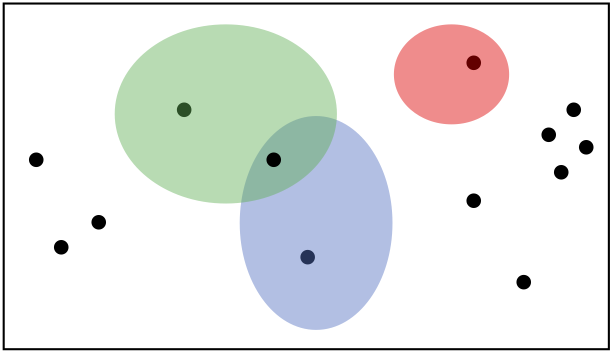
\includegraphics[width=2.5in]{venndiagram-cropped.png}
\caption{The universe of possible attacks against a cryptographic scheme or
protocol.} 
\label{fig:venndiagram}
\end{wrapfigure}


This is not to say that theory, modeling, and formal analysis aren't critical to
applied cryptography. Most obviously we will be building off the deep literature
from theoretical cryptography, and without that theory we would be lost. More
directly, theory provides us powerful tools to help us rule out large
classes of attacks for deployed schemes, that complement and strengthen the one-at-a-time
approach of simple attack-driven investigations. 
One can visualize this process for a particular
scheme as shown in \figref{fig:venndiagram}, which means to depict the universe of all
possible attacks and those attacks covered by different analysis approaches. Each point in
this universe represents an implementable attack against an instantiation 
of the system, which may or may not succeed, and the goal of the analyst is to rule out
the efficacy of as many such attacks as possible.  The black dots
represent one-at-a-time investigation ruling out individual attacks, the
green circle might represent formal reduction-based analyses, the blue circle
symbolic analyses, and the red circle an analysis of some class of side-channel
attacks.  Of course this is highly abstracted, but gives a sense of the
thinking: formal modeling and analysis can help rule out larger classes of
attacks, but certainly will miss things that fall outside the scope of the
model. By combining approaches in a thoughtful manner combined with normative
intuition, one achieves better coverage and can spot attack strategies that may
be more likely to work.

To make this kind of approach work, though, we must have a mastery of modeling
and formal analysis tools. Gaining that mastery is the subject of this course.






\newpage
%%%%%%%%%%%%%%%%%%%%%%%%%%%%%%%%%%%%%%%%%%%%%%%%%%%%%%%%%%%%%%%%%%%%%%%%%%%%%%%%
\section{Preliminaries and Notation}
\label{sec:notation}

We collect here some notation that we will use throughout these notes. 
\tnote{If you introduce new notation in writing up a lecture, please consider
adding it here.} 


\paragraph{Basics.}
We most often denote sets by calligraphic, capital letters, such as $\calX$,
$\calY$, $\calZ$. A discrete probability distribution is a set $\Omega$, the
event space, together with a
function~$p\Colon\Omega\rightarrow[0,1]$ for which $\sum_{\omega\in\Omega}
p_\Omega(\omega) = 1$.
We write $p_\Omega$ when we need to disambiguate the event space, but
otherwise simply $p$ when $\Omega$ is clear from context. We will also,
following convention, often write $\Pr[\omega]$ instead of $p(\omega)$.
The support of $p$ is defined to be the set $\supp(p) = \{\omega \;|\; \omega
\in \Omega \land p(\omega) > 0\}$, 
i.e., the set of all points in $\Omega$ that have non-zero probability.  
As a slight abuse of notation, we can write 
$\Pr[\calS] = p(\calS) = \sum_{\omega\in\calS} p(\omega)$ for any set $\calS \subseteq \Omega$. 

A random variable $X$ is a map $Y\Colon\Omega\rightarrow\calX$ from some event
space $\Omega$ with associated probability distribution $p_\Omega$ over a  set
$\Omega$. So for some other set $\calS$ we let $\Pr[X\in\calS] = \Pr[\{\omega
\;|\; X(\omega) \in \calS\}]$ to be the probability that the random variable
takes on a value in $\calS$, over the probability distribution $p_\Omega$.

We use the language of probability as the foundation for formalizing
cryptographic algorithms, security, and more. Interestingly the probability
spaces involved get complicated quickly, and a common problem is that they end 
ambiguous. We will therefore rely on a crutch that has proved quite useful for
communicating, and reasoning about, probability distributions.


\paragraph{Pseudocode games.} We fix some pseudocode language to describe
security models, cryptographic algorithms, and more. Roughly we will follow the
notational tradition established by Bellare and Rogaway in the
2000s~\cite{bellare2006security}, but using slightly different syntax/symantecs that are
based most closely on a treatment from~\cite{ristenpart2011careful}.  Code-based
games are convenient for more precisely defining probability spaces, which are
what we use to model security and correctness goals, algorithms, and more.  

%We follow~\cite{BR06} 
%with some differences.
We will use procedures, variables, and typical
programming statements (such as operators, loops, procedure calls, etc.).
Typical statements are shown in \figref{fig:statements}.
We do not provide a formal specification of the programming language,
see~\cite[Appendix B]{bellare2006security} for an example of doing so. 
%Games include
%procedures, variables, and typical programming 
%statements (operators, loops, etc.). 
We will rely on some conventions to help make sense of games.
Types should be understable
from context. The names of syntactic objects (procedures, variables, etc.)
must be distinct.  Variables are implicitly 
initialized to default values:  integer variables are set
to 0, arrays are everywhere~$\bot$, etc. Here $\bot$ is a distinguished symbol
by tradition used to denote an error in the cryptographic literature.
By distinguished we mean that it assumed to not be used for any other reason,
not appearing in alphabets over which strings are taken, etc.


\begin{wrapfigure}{r}{3in}
\gamesfontsize
\begin{tabular}{lp{2in}}
\toprule
$x \gets y$ & Assignment\\
$x \getsr \calX$ & Uniform sampling from a set\\
$z \getsr P(x,y)$ & Call a randomized procedure\\
$z \gets P(x,y)$ & Call a deterministic procedure\\
Ret $x$ & Return from a procedure\\
$z \gets x \concat y$ & String concatenation\\
$(x,y) \getparse{n} z$ & Parse string $z$ s.t.~$|x| = n$\\
\bottomrule
\end{tabular}
\caption{Some statements used in our games.}
\label{fig:statements}
\end{wrapfigure}


A \textit{procedure} is a sequence of statements together 
with zero or more variable inputs and zero or more 
outputs. %
%Variables are by default local, meaning they can only be 
%used within a single procedure, but they retain their state 
%between calls to the procedure. %
An \emph{unspecified procedure} is a procedure whose pseudocode, inputs, and
outputs are understood from context.  We will see some examples of
unspecified procedures, the most frequent in our security games being the 
\emph{adversary} which is often left unspecified. 
%
%
A call to a procedure requires providing it with inputs, running its sequence of
statements, and returning its output. We will interchangeably use the term call
and \emph{query} for procedure invocation.
A procedure~$P$ can itself query other
procedures. The set of procedures $Q_1,\ldots,Q_k$ called by a procedure are
statically fixed, and we require that there are no type mismatches in inputs and
outputs. 

Say that the code of~$P$ expects to be able to call~$k$ distinct procedures.
We will write $P^{Q_1,Q_2,\ldots,Q_k}$ to denote that these calls are
handled by $Q_1,Q_2,\ldots,Q_k$ and implicitly assume (for all $i\in[k]$) that there are no
syntactic mismatches between the calls that~$P$ makes to~$Q_i$ and the inputs
of~$Q_i$, as well as between the return values of~$Q_i$
and the return values expected by~$P$.   
%We stress that~$P$ does not
%call~$Q_i$ by name, but rather calls to a procedure that is
%instantiated by~$Q_i$.

We assume that all procedures eventually halt, regardless of randomness used, 
returning their outputs, at which point execution returns to the 
calling procedure.
Two procedures~$P_1$ and~$P_2$ are said to 
\emph{export the same interface} 
if their inputs and outputs have the same number and types. 

Variables will be local by default, meaning they can only be used within a
single procedure. Variables are static, meaning that they retain their 
state between calls to the procedure. It will be convenient to 
allow sharing of variables at times, for which we use a 
\textit{collection of procedures}. This is a set 
of one or more procedures whose variables have scope covering all of the
procedures. We will denote a collection of procedures using 
a common prefix ending with a period, so for example~$(P.x,P.y,\ldots)$,
Sometimes we will use the term interfaces for the specific prefixes of the a
collection of procedures~$P$. 

A \emph{main procedure} is a special procedure that takes no inputs and has some
output.  We will mark it by \main{} (though below
we'll see some syntactic sugar that provides greater brevity).  No procedure may
call~\main{}, it can access all the variables of other specified procedures
(though not unspecified procedures). 

A game consists of a main procedure together with a set of zero or more
specified procedures. We write $\G$ for a game. A game may also make use of
unspecified procedures (such as adversaries), which we enumerate as
superscripts, e.g., $\G^{P_1,P_2,\ldots,P_k}$. In most games used as security
definitions, one (or more) of the unspecified procedures will be called the
adversary, most often denoted by~$\advA$. For a given instantiation of the
unspecified procedures, one can run a game: execute its
statements starting with the designated \main{} procedure, and ultimately
outputing whatever \main{} returns.  

\paragraph{Run times and random variables.} Games can make random choices, due
to the supported statements for sampling according to a distribution. We can
associate to games a model of computation, which specifies how much running each
(type of) statement costs in terms of time, memory, or both.   A typical model
is to assign to each statement the same abstract unit cost, and the run time
then becomes the number of statements executed in the course of the game. 
When procedures are called, we attribute the unit cost of the call statement to
the caller and the remaining cost of executing the procedure's statements to the
callee. 

By default we will require that games terminate in some finite number of
steps~$\runtime$, and clarify explicitly when this does not hold. The number of
queries made by the main procedure, or any other procedure for that matter
including unspecified ones, is
therefore also upper bound by $\runtime$. We  may often limit the number of
queries made by an adversary to some maximum number $\numqueries \le \runtime$. 

Given these finiteness conditions, we similarly know that there is a finite
limit on the number of random samples made in a game. Since we restricted to 
random sampling from finite sets, we have that for any game $\G$ 
there is an event space~$\Omega_\G$ and an associated probability distribution
defining the output of the game $\G$. Given our restrictions, $\Omega_\G$ is a
set of possible values, the cross-product of all the random sampling procedures
within $\G$. We sometimes refer to $\Omega_\G$ as the \emph{coins} of the game.
For some fixed unspecified procedures
$P_1,\ldots,P_k$ we denote the event that executing the game
$\G^{P_1,\ldots,P_k}$ outputs a particular value $y$ by
``$\G^{P_1,\ldots,P_k}\Rightarrow y$'' and the associated probability over
$\Omega_\G$ is denoted $\Pr[\G^{P_1,\ldots,P_k}\Rightarrow y]$. When $y$ is clear
from context we will omit it, writing instead $\Pr[\G^{P_1,\ldots,P_k}]$.  
For example, we will often have games output a boolean and then
$y$ will most often be the value \true.

We can similarly associate to any variable within a game an event within
$\Omega_\G$. These can also be equivalently considered to be random variables on
domain $\Omega_G$. Our convention will be to overload notation, and define the
event that a variable $X$ in a game $\G$ takes on a certain value $y$ as simply
``$X = y$'' with associated probability $\Pr[X = y]$ over the coins of
$\Omega_\G$. 


\paragraph{Runnable games.}  We want to emphasize a point, which is that games
are by our conventions above runnable. That means that, once any unspecified
procedures are fixed, you could write a program in a conventional programming
language, and actually run the game on a real computer. Obviously like with all
abstract algorithms, the actual run times will vary, but assuming relative
efficiency the game will complete.  

It relatively frequently arises in proofs that one deviates from runnable games.
A common example is logic of the following form. Let $\advA$ be an adversary,
and consider a game $\G^\advA$. Remember we implicitly assume that $\advA$ is
compatible with $\G$, and we have that $\G^\advA$ is runnable.  Now consider the
set of all adversaries compatible with $\advA$, and let $\advA_{\max}$ be the
member of this set that maximizes $\Pr[\G^\advA \Rightarrow \true]$. But now
$\G^{\advA_{\max}}$ is no longer runnable, because $\advA_{\max}$ is not
concretely specified. While mathematically $\advA_{\max}$ is well-defined, there
is no clear way to write down its code, even given the code defining~$\advA$.
We will try whenever possible to avoid such arguments, as they have various
subtle implications that are, in general, not great for making 
clear claims about security. 






%\newpage
%%%%%%%%%%%%%%%%%%%%%%%%%%%%%%%%%%%%%%%%%%%%%%%%%%%%%%%%%%%%%%%%%%%%%%%%%%%%%%%%%
\section{Ciphers and Initial Security Notions}
\label{sec:se}

\paragraph{Ciphers.}
We start by defining a cipher. A cipher $\cipher = (\cipherE,\cipherD)$ is
defined by a a pair of deterministic algorithms $\cipherE$ and $\cipherD$.  To
any cipher $\cipher$ we associate sets called the key space $\keyspace$, message
space $\msgspace$, and ciphertext space $\ctxtspace$. We do not surface in the
notation for a cipher these sets, and will require that the association be clear
from context.

The algorithms are two-input. Enciphering takes a key $K \in \keyspace$ and
message $M \in \msgspace$, and outputs a ciphertext $C \in \ctxtspace$. Because
$\cipherE$ is deterministic, we can equally formalize it as a map 
$\cipherE\Colon\keyspace\times\msgspace\rightarrow\ctxtspace$. For a given key
$K$ we let $\cipherE_K\Colon\msgspace\rightarrow\ctxtspace$ be defined by
$\cipherE_K(M) = \cipherE(K,M)$ for all $M \in \msgspace$.  Deciphering takes a key $K\in \keyspace$ and ciphertext
$C \in \ctxtspace$ and outputs a message $M \in \msgspace$. Again, we can view
it as a map $\cipherD\Colon\keyspace\times\ctxtspace\rightarrow\msgspace$. 

Both $\cipherE$ and $\cipherD$ must be efficiently computable for all $K \in
\keyspace$.  (We have not defined efficiently computable, and use the term here
informally.) We require that a cipher be correct, meaning that for
$\cipherD_K(\cipherE_K(M)) = M$ for all $M$. 

\paragraph{Security notions.} What do we intuitively expect of a cipher?
Minimally:
\begin{itemize}
\item Secret key should remain secret
\item Message should remain secret
\end{itemize}
Let's try to formalize these notions.
\begin{itemize}
\item TKR security
\item KR security
\item (ot-)IND security
\end{itemize}


\begin{figure}[p]
\fpage{.45}{
\underline{$\TKR^\advA_\cipher$}\\[1pt]
$K \getsr \keyspace$\\
$K^* \getsr \advA^\Fn$\\
Ret $(K = K^*)$\medskip

\underline{$\Fn(M)$}\\
$C \gets \cipherE_K(M)$\\
Ret $C$
}
\end{figure}

We let $\TKR_\cipher$-advantage of a $\TKR_\cipher$-adversary $\advA$ be defined by 
\bnm
  \AdvTKR{\cipher}{\advA} = \Prob{\TKR^\advA_\cipherE \Rightarrow\true}  \;.
\enm

\begin{figure}[p]
\fpage{.45}{
\underline{$\KR^\advA_\cipher$}\\[1pt]
$K \getsr \keyspace$\\
$K^* \getsr \advA^\Fn$\\
$\win \gets \true$\\ 
For $M \in \calX$:\\
\ind If $\cipherE_{K^*}(M) \ne \cipherE_{K}(M)$ then\\
\ind\ind $\win \gets \false$\\
Ret $\win$\medskip

\underline{$\Fn(M)$}\\
$\calX \gets \calX \cup \{M\}$\\
$C \gets \cipherE_K(M)$\\
Ret $C$
}
\end{figure}

We let $\KR_\cipher$-advantage of a $\KR_\cipher$-adversary $\advA$ be defined by 
\bnm
  \AdvKR{\cipher}{\advA} = \Prob{\KR^\advA_\cipherE \Rightarrow\true}  \;.
\enm


\begin{figure}[p]
\fpage{.45}{
\underline{$\OTIND^\advA_\cipher$}\\[1pt]
$K \getsr \keyspace$\\
$b \getsr \bits$\\
$b' \getsr \advA^\Fn$\\
Ret $(b = b')$\medskip

\underline{$\Fn(M_0,M_1)$}\\
$C \gets \cipherE_K(M_b)$\\
Ret $C$
}
\end{figure}

We let $\OTIND_\cipher$-advantage of a $\OTIND_\cipher$-adversary $\advA$ be defined by 
\bnm
  \AdvOTIND{\cipher}{\advA} = 2\cdotsm\Prob{\OTIND^\advA_\cipherE \Rightarrow\true} - 1  \;.
\enm

\bigskip
\bigskip


\begin{itemize}
\item First example: Our simple OTP cipher is not $\TKR$ secure? Go over example: $\advA$
queries once on arbitrary message, recovers $K$ by computing $M \oplus C$. This
is guaranteed to succeed because $M \oplus C$ uniquely defines $K$. What does
this mean? Isn't OTP considered secure? Shannon said so!
%
\item Second example: Give toy cipher $\cipher$ for which $\TKR_\cipher$ has
$\AdvTKR{\cipher}{\advA} = 0$ for any adversary $\advA$. What is it?
$\cipherE(K,M) = M$. It is correct 
%
\item Third example: Exhaustive key search attack against generic
cipher. Emphasize that lower-bounding the efficacy of this is not possible in
general. Why? Consider toy identity cipher! 
%
\item Discuss the KR definition. Rules out the
identity map as being relevant. Lower-bounding security is 
%
\item Shannon's perfect secrecy (one-time left-or-right indistinguishability). 
\end{itemize}

\begin{theorem}
Let $\cipher$ be a cipher. For any $\TKR_\cipher$-adversary $\advA$, we give a
$\KR_\cipher$-adversary $\advB$ such that 
  $\AdvKR{\cipher}{\advA} = \AdvTKR{\cipher}{\advB}$.
\end{theorem}

In our theorem statements including reductions,  we need to interpret the words
``we give a''. We will focus on concrete, specified reductions. That means that
the adversary $\advB$ not only exists, but is fully specified  --- minus the
details of $\advA$ ---  within the proof.  In particular, if you give someone
$\advA$ then $\advB$ becomes runnable.  Runnable reductions are generally
speaking easier to interpret when it comes to implied security guarantees. They
even allow us to use the human-ignorance model~\cite{rogaway2006formalizing}
which, roughly, states that a reduction even to a mathematically easy assumption
can still be meaningful. (We will revisit this particular issue with an example
in the context of collision resistance.)
An example of a non-runnable $\advB$ would be one that includes some constant
value that we know exists, but don't know an exact value for. This comes up in
various arguments, and can cause problems in interpreting the reduction in terms
of concrete security.  This issue is subtle and we will revisit it.

The takeaway here being that one interprets ``we give a'' to mean runnable
adversaries that are specified fully in the proof. (Or when brevity is at stake,
specified to a leave of detail that the average reader could specify it in
detail easily.)  When we deviate from this convention we should remark on it.




\begin{theorem}
Let $\cipher$ be the OTP cipher. Then for any single-query
$\OTIND_\cipher$-adversary $\advA$ it holds that $\AdvOTIND{\cipher}{\advA} = 0$. \end{theorem}


\begin{theorem}
Let $\cipher$ be a cipher defined 
over $(\keyspace,\msgspace,\ctxtspace)$ such that for any $\OTIND_\cipherE$-adversary 
$\advA$ it holds that $\AdvOTIND{\cipher}{\advA} = 0$. Then $|\keyspace| \ge
|\msgspace|$. 
\end{theorem}


\begin{figure}
\fpage{.45}{
\underline{$\advA_{\textrm{eks}}$}\\[1pt]
$C \gets \Fn(M)$\\
For $K \in \calK$ do:\\
\ind If $C = \cipherE(K,M)$ then\\
\ind\ind Return $K$\\
Return $\bot$
}
\end{figure}

\paragraph{PRPs and PRFs.}

\begin{itemize}
\item Basic cipher definitions, key recovery attacks
\item PRP and PRF definitions
\item PRP/PRF switching lemma
\begin{itemize}
  \item Incorrect conditioning argument 
  \item Correct game-playing argument
\end{itemize}
\item PRP from PRF constructions: Feistel networks
\item Luby-Rackoff proof
\end{itemize}


\begin{figure}
\fpage{.15}{
\underline{$\PRP_{\cipher}^\advA$}\\
$b \getsr \bits$\\
$K \getsr \keyspace$\\
$\pi \getsr \Perm(n)$\\
$b' \getsr \advA^\Fn$\\
Return $(b = b')$\medskip

\underline{$\Fn(M)$}\\
If $b = 1$ then\\
\ind Return $\cipherE_K(M)$\\
Return $\pi(M)$
}
\end{figure}

\bnm
\AdvPRP{\cipher}{\advA} = 2\cdotsm\Prob{\PRP^\advA_\cipher\Rightarrow\true}- 1
\enm

\begin{figure}
\hfpages{.25}{
\underline{$\PRP1_{\cipher}^\advA$}\\
$K \getsr \keyspace$\\
$b' \getsr \advA^\Fn$\\
Return $b'$\medskip

\underline{$\Fn(M)$}\\
Return $\cipherE_K(M)$\\
}{
\underline{$\PRP0_{\cipher}^\advA$}\\
$\pi \getsr \Perm(n)$\\
$b' \getsr \advA^\Fn$\\
Return $b'$\medskip

\underline{$\Fn(M)$}\\
Return $\pi(M)$\\
}


\end{figure}


\begin{figure}
\hfpages{.25}{
\underline{$\PRF1_{\cipher}^\advA$}\\
$K \getsr \keyspace$\\
$b' \getsr \advA^\Fn$\\
Return $b'$\medskip

\underline{$\Fn(M)$}\\
Return $\cipherE_K(M)$\\
}{
\underline{$\PRF0_{\cipher}^\advA$}\\
$\rho \getsr \Func(n,n)$\\
$b' \getsr \advA^\Fn$\\
Return $b'$\medskip

\underline{$\Fn(M)$}\\
Return $\rho(M)$\\
}


\end{figure}



\begin{lemma} Let $\cipher$ be a cipher with ciphertext space $\bits^n$. 
Let $\advA$ be an adversary making at most $q$ queries. Then
\bnm
  \left| \Prob{\PRF0_\cipher^\advA\Rightarrow 1} 
      - \Prob{\PRP0_\cipher^\advA\Rightarrow1} \right| \le \frac{q^2}{2^n}  \;.
\enm
\end{lemma}

\begin{align*}
&\left| \Prob{\PRP0_\cipher^\advA\Rightarrow 1} 
      - \Prob{\PRF0_\cipher^\advA\Rightarrow1} \right| \\ 
     &\myInd\myInd\myInd =  \left|\Prob{\G0} - \Prob{\PRF0_\cipher^\advA\Rightarrow1} \right|  \\
     &\myInd\myInd\myInd  =  \left|\Prob{\G1} - \Prob{\PRF0_\cipher^\advA\Rightarrow1} \right|  \\
     &\myInd\myInd\myInd  \le \left|\Prob{\G2} + \Prob{\bad_2} - \Prob{\PRF0_\cipher^\advA\Rightarrow1} \right|\\
     &\myInd\myInd\myInd  = \Prob{\bad_2}\\
     &\myInd\myInd\myInd  \le \frac{q^2}{2^n}\\
\end{align*}

\begin{lemma} Let $\G$, $\Hgame$ be games that are identical-until-bad and $y$ be any
value. Then
\bnm
  \big| \Prob{\G\Rightarrow y} 
      - \Prob{\Hgame\Rightarrow y} \big| \le \Prob{\Hgame\setsbad} = \Prob{\G\setsbad}  \;.
\enm
\end{lemma}


\begin{figure}
\hfpagess{.20}{.20}{
\underline{$\G0$}\\[2pt]
$b' \getsr \advA^\Fn$\\
Return $b'$\medskip

\underline{$\Fn(M)$}\\
If $\TabF[M] = \bot$ then\\
\ind $\TabF[M] \getsr \bits^n \setminus \TabF$\\
Return $\TabF[M]$
}{
\underline{\fbox{$\G1$} \;\;\; $\G2$}\\[2pt]
$b' \getsr \advA^\Fn$\\
Return $b'$\medskip

\underline{$\Fn(M)$}\\
$C \getsr \bits^n$\\
If $C \in \TabF$ then\\
\ind $\badtrue$\\
\ind \fbox{$C \getsr \bits^n \setminus \TabF$}\\
$\TabF[M] \gets C$\\
Return $\TabF[M]$
}


\end{figure}



\begin{figure}
\hfpagessss{.20}{.20}{.20}{.20}{
\underline{$\G0$}\\[2pt]
$K \getsr \bits^k$\\
$b' \getsr \advA^\Fn$\\
Return $b'$\medskip

\underline{$\Fn(LR)$}\\
$L_1 \gets R$\\
$R_1 \gets L \oplus F_K(\langle 1\rangle \concat R)$\\
$L_2 \gets R_1$\\
$R_2 \gets L_1 \oplus F_K(\langle 2 \rangle \concat R_1)$\\
$L_3 \gets R_2$\\
$R_3 \gets L_2 \oplus F_K(\langle 3 \rangle \concat R_2)$\\
Return $L_3 \concat R_3$
}{
\underline{$\G1$}\\[2pt]
$\rho \getsr \Func(2n,n)$\\
$b' \getsr \advA^\Fn$\\
Return $b'$\medskip

\underline{$\Fn(LR)$}\\
$L_1 \gets R$\\
$R_1 \gets L \oplus \rho(\langle 1\rangle \concat R)$\\
$L_2 \gets R_1$\\
$R_2 \gets L_1 \oplus \rho(\langle 2 \rangle \concat R_1)$\\
$L_3 \gets R_2$\\
$R_3 \gets L_2 \oplus \rho(\langle 3 \rangle \concat R_2)$\\
Return $L_3 \concat R_3$
}{
\underline{$\fbox{\G2}$\;\;\;\G3}\\[2pt]
$b' \getsr \advA^\Fn$\\
Return $b'$\medskip

\underline{$\Fn(LR)$}\\
$L_1 \gets R$\\
If $\TabF[1,R] = \bot$ then\\
\ind $\TabF[1,R] \getsr \bits^n$\\
$R_1 \gets L \oplus \TabF[1,R]$\\
$L_2 \gets R_1$\\
$X_2 \getsr \bits^n$\\
If $\TabF[2,R_1] \ne \bot$ then\\
\ind $\badtrue$\\
\ind \fbox{$X_2 \gets \TabF[2,R_1]$}\\
$\TabF[2,R_1] \gets X_2$\\
$R_2 \gets L_1 \oplus X_2$\\
$L_3 \gets R_2$\\
$X_3 \getsr \bits^n$\\
If $\TabF[3,R_2] \ne \bot$ then\\
\ind $\badtrue$\\
\ind \fbox{$X_3 \gets \TabF[2,R_2]$}\\
$\TabF[3,R_2] \gets X_3$\\
$R_3 \gets L_2 \oplus X_3$\\
Return $L_3 \concat R_3$
}{
\underline{$\G4$}\\[2pt]
$b' \getsr \advA^\Fn$\\
Return $b'$\medskip

\underline{$\Fn(LR)$}\\
$L_1 \gets R$\\
If $\TabF[1,R] = \bot$ then\\
\ind $\TabF[1,R] \getsr \bits^n$\\
$R_1 \gets L \oplus \TabF[1,R]$\\
$L_2 \gets R_1$\\
If $\TabF[2,R_1] \ne \bot$ then\\
\ind $\badtrue$\\
$\TabF[2,R_1] \gets 1$\\
$R_2 \getsr \bits^n$\\
$L_3 \gets R_2$\\
%$X_3 \getsr \bits^n$\\
If $\TabF[3,R_2] \ne \bot$ then\\
\ind $\badtrue$\\
$\TabF[3,R_2] \gets 1$\\
$R_3 \getsr \bits^n$\\
Return $L_3 \concat R_3$
}
\end{figure}

\begin{figure}
\fpage{.25}{
\underline{$\advB^\Fn$}\\[2pt]
$K \getsr \bits^k$\\
$b' \getsr \advA^\FnSim$\\
Return $b'$\medskip

\underline{$\FnSim(LR)$}\\
$L_1 \gets R$\\
$R_1 \gets L \oplus \Fn(\langle 1\rangle \concat R)$\\
$L_2 \gets R_1$\\
$R_2 \gets L_1 \oplus \Fn(\langle 2 \rangle \concat R_1)$\\
$L_3 \gets R_2$\\
$R_3 \gets L_2 \oplus \Fn(\langle 3 \rangle \concat R_2)$\\
Return $L_3 \concat R_3$
}
\end{figure}

\newpage

\begin{theorem}
Let $\Feistel$ be the 3-round Feistel cipher using round function 
$F\Colon\bits^k\times\bits^n\rightarrow \bits^n$. For any
$\PRP_\cipher$-adversary $\advA$ making at most $q$ queries 
we give an $\PRF_F$-adversary $\advB$ making at most $3q$ queries such that
\bnm
  \AdvPRP{\Feistel}{\advA} \le \AdvPRF{F}{\advB} + \frac{2q^2}{2^n} +
  \frac{q^2}{2^{2n}} \;.
\enm
\end{theorem}



\begin{align*}
\AdvPRP{\cipher}{\advA} 
    &= \left|\Prob{\PRP1^\advA_\cipher} - \Prob{\PRP0^\advA_\cipher}\right|\\
    &= \left|\Prob{\G0} - \Prob{\PRP0^\advA_\cipher}\right|\\
    &\le \left|\Prob{\G1} + \AdvPRF{F}{\advB} - \Prob{\PRP0^\advA_\cipher}\right|\\
    &=   \left|\Prob{\G2} + \AdvPRF{F}{\advB} - \Prob{\PRP0^\advA_\cipher}\right|\\
    &\le \left|\Prob{\G3} + \Prob{\bad_3} + \AdvPRF{F}{\advB} - \Prob{\PRP0^\advA_\cipher}\right|\\
    &= \left|\Prob{\G4} + \Prob{\bad_4} + \AdvPRF{F}{\advB} - \Prob{\PRP0^\advA_\cipher}\right|\\
    &\le \left|\Prob{\PRP0^\advA_\cipher} + \frac{q^2}{2^{2n}} + \Prob{\bad_4} + \AdvPRF{F}{\advB} - \Prob{\PRP0^\advA_\cipher}\right|\\
    &= \frac{q^2}{2^{2n}} + \Prob{\bad_4} + \AdvPRF{F}{\advB}\\
    &\le \frac{q^2}{2^{2n}} + \frac{2q^2}{2^n} + \AdvPRF{F}{\advB}\\
\end{align*}


\newpage
%%%%%%%%%%%%%%%%%%%%%%%%%%%%%%%%%%%%%%%%%%%%%%%%%%%%%%%%%%%%%%%%%%%%%%%%%%%%%%%%
\section{Ciphers and Initial Security Notions}
\label{sec:se}

\paragraph{Ciphers.}
We start by defining a cipher. A cipher $\cipher = (\cipherE,\cipherD)$ is
defined by a a pair of deterministic algorithms $\cipherE$ and $\cipherD$.  To
any cipher $\cipher$ we associate sets called the key space $\keyspace$, message
space $\msgspace$, and ciphertext space $\ctxtspace$. We do not surface these sets in the
notation for a cipher, and we will require that the association be clear
from context.

Each algorithm has two inputs. Enciphering takes a key $K \in \keyspace$ and
message $M \in \msgspace$, and outputs a ciphertext $C \in \ctxtspace$. Because
$\cipherE$ is deterministic, we can equally formalize it as a map 
$\cipherE\Colon\keyspace\times\msgspace\rightarrow\ctxtspace$. For a given key
$K$ we let $\cipherE_K\Colon\msgspace\rightarrow\ctxtspace$ be defined by
$\cipherE_K(M) = \cipherE(K,M)$ for all $M \in \msgspace$.  Deciphering takes a key $K\in \keyspace$ and ciphertext
$C \in \ctxtspace$ and outputs a message $M \in \msgspace$. Again, we can view
it as a map $\cipherD\Colon\keyspace\times\ctxtspace\rightarrow\msgspace$. 

Both $\cipherE$ and $\cipherD$ must be efficiently computable for all $K \in
\keyspace$.  (We have not defined efficiently computable and use the term here
informally.) We require that a cipher be correct, meaning that
$\forall M \in \msgspace, \forall K \in \keyspace, \cipherD_K(\cipherE_K(M)) = M$.

\paragraph{Example.} One simple example of a cipher is the \textbf{one-time pad} (OTP). Let $\keyspace = \msgspace=\ctxtspace=\{0,1\}^n$ for some $n \in \N$. Then we define OTP as follows:
\begin{align*}
&\cipherE_K(M) = M \oplus K \\
&\cipherD_K(C) = C \oplus K
\end{align*}
Claude Shannon proved that OTP is perfectly secure in 1949 \cite{shannon1949communication}.

\paragraph{Security notions.} What do we intuitively expect of a cipher?
Minimally:
\begin{itemize}
\item The secret key should remain secret.
\item The message should remain secret.
\end{itemize}

Let's try to formalize these notions. We will start with a security notion called \textbf{target key recovery security} (TKR).
As the name suggests, the goal of the adversary is to recover the challenge key given a chosen plaintext attack, meaning the adversary can choose which messages to query to the $\Fn$ oracle. The game pseudocode is provided in \figref{fig:tkr}. We let $\TKR_\cipher$-advantage of a $\TKR_\cipher$-adversary $\advA$ be defined by 
\bnm
\AdvTKR{\cipher}{\advA} = \Prob{\TKR^\advA_\cipherE \Rightarrow\true}  \;.
\enm

\begin{figure}[p]
	\centering
	\fpage{.45}{
		\underline{$\TKR^\advA_\cipher$}\\[1pt]
		$K \getsr \keyspace$\\
		$K^* \getsr \advA^\Fn$\\
		Ret $(K = K^*)$\medskip
		
		\underline{$\Fn(M)$}\\
		$C \gets \cipherE_K(M)$\\
		Ret $C$
	}
	\caption{The target key recovery game.}
	\label{fig:tkr}
\end{figure}


We must now ask ourselves how well TKR captures the security of a cipher. Let us first try to analyze the security of OTP using this definition. Notice that OTP actually fails to provide TKR security, which we show with the following adversary.
\begin{align*}
&\underline{\textbf{adversary } \advA} \\
&K \gets \Fn(0^n) \\
&\text{Return } K 
\end{align*}	

$\advA$ simply queries for $0^n$, which returns $0^n \oplus K = K$, thereby recovering the challenge key with $\AdvTKR{\cipher}{\advA} = 1$. This then means that OTP is actually insecure according to the TKR security definition. But as we noted earlier, OTP is considered secure! Our definition then fails to capture the security of OTP. 

Now consider the identity cipher $\cipherE_{K}(M) = M$ for $\keyspace=\{0,1\}^k$. Since the cipher simply returns the message, no information about the key is included in the ciphertext. The best an adversary can do is return a random key, which has probability $2^{-k}$ of being the correct target key.
Then for any adversary $\advA$, it holds that $\AdvTKR{\cipher}{\advA} = 2^{-k}$, meaning the identity cipher is secure! Clearly this is not the case, and thus TKR security does not provide message confidentiality. Furthermore, this security notion is ``unfair'' to an adversary, since there can be many keys that are \textit{consistent} on a query transcript. 

\begin{figure}[p]
	\centering
	\fpage{.45}{
		\underline{$\KR^\advA_\cipher$}\\[1pt]
		$\win \gets \false$\\
		$K \getsr \keyspace$\\
		$K^* \getsr \advA^\Fn$\\ 
		For $M \in \calX$:\\
		\ind If $\cipherE_{K^*}(M) \ne \cipherE_{K}(M)$ then\\
		\ind\ind $\win \gets \false$\\
		Return $\win$\medskip
		
		\underline{$\Fn(M)$}\\
		$\win \gets \true$ \\
		$\calX \gets \calX \cup \{M\}$\\
		$C \gets \cipherE_K(M)$\\
		Ret $C$
	}
	\caption{The key recovery game.}
	\label{fig:kr}
\end{figure}

We then look at a different notion called \textbf{key recovery security} (KR). Under this definition, if an adversary outputs a key that is consistent with the query transcript, then it wins. The game pseudocode is provided in \figref{fig:kr}. We let $\KR_\cipher$-advantage of a $\KR_\cipher$-adversary $\advA$ be defined by 
\bnm
\AdvKR{\cipher}{\advA} = \Prob{\KR^\advA_\cipherE \Rightarrow\true}  \;.
\enm

\paragraph{Comparing security definitions.} We can formally compare security definitions. To show that some definition DEF1 does not imply another definition DEF2, we can show a \textit{counter-example}. This requires producing a scheme such that we can show that no (reasonable) DEF1-adversary has a good advantage. We then give a DEF2-adversary that gets good DEF2 advantage.

Conversely, to show that DEF1 does imply DEF2, we can show a \textit{reduction}. This requires converting a DEF2-adversary $\advA$ into a DEF1-adversary $\advB$ such that $\advB$'s DEF1 advantage upper bounds $\advA$'s DEF2 advantage. 


\begin{table}
	\centering
	\begin{tabular}{c | c}
		DEF1 $\not \Rightarrow$ DEF2 & We show a counter-example. \\ \hline
		DEF1 $\Rightarrow$ DEF2 & We show a reduction.
	\end{tabular}
\end{table}

\begin{itemize}
	\item First example: Our simple OTP cipher is not $\TKR$ secure? Go over example: $\advA$
	queries once on arbitrary message, recovers $K$ by computing $M \oplus C$. This
	is guaranteed to succeed because $M \oplus C$ uniquely defines $K$. What does
	this mean? Isn't OTP considered secure? Shannon said so!
	%
	\item Second example: Give toy cipher $\cipher$ for which $\TKR_\cipher$ has
	$\AdvTKR{\cipher}{\advA} = 0$ for any adversary $\advA$. What is it?
	$\cipherE(K,M) = M$. It is correct 
	%
	\item Third example: Exhaustive key search attack against generic
	cipher. Emphasize that lower-bounding the efficacy of this is not possible in
	general. Why? Consider toy identity cipher! 
	%
	\item Discuss the KR definition. Rules out the
	identity map as being relevant. Lower-bounding security is 
	%
	\item Shannon's perfect secrecy (one-time left-or-right indistinguishability). 
\end{itemize}


\begin{itemize}
	\item KR security
	\item (ot-)IND security
\end{itemize}


\begin{figure}[p]
\fpage{.45}{
\underline{$\OTIND^\advA_\cipher$}\\[1pt]
$K \getsr \keyspace$\\
$b \getsr \bits$\\
$b' \getsr \advA^\Fn$\\
Ret $(b = b')$\medskip

\underline{$\Fn(M_0,M_1)$}\\
$C \gets \cipherE_K(M_b)$\\
Ret $C$
}
\end{figure}

We let $\OTIND_\cipher$-advantage of a $\OTIND_\cipher$-adversary $\advA$ be defined by 
\bnm
  \AdvOTIND{\cipher}{\advA} = 2\cdotsm\Prob{\OTIND^\advA_\cipherE \Rightarrow\true} - 1  \;.
\enm

\bigskip
\bigskip




\begin{theorem}
Let $\cipher$ be a cipher. For any $\TKR_\cipher$-adversary $\advA$, we give a
$\KR_\cipher$-adversary $\advB$ such that 
  $\AdvKR{\cipher}{\advA} = \AdvTKR{\cipher}{\advB}$.
\end{theorem}

In our theorem statements including reductions,  we need to interpret the words
``we give a''. We will focus on concrete, specified reductions. That means that
the adversary $\advB$ not only exists, but is fully specified  --- minus the
details of $\advA$ ---  within the proof.  In particular, if you give someone
$\advA$ then $\advB$ becomes runnable.  Runnable reductions are generally
speaking easier to interpret when it comes to implied security guarantees. They
even allow us to use the human-ignorance model~\cite{rogaway2006formalizing}
which, roughly, states that a reduction even to a mathematically easy assumption
can still be meaningful. (We will revisit this particular issue with an example
in the context of collision resistance.)
An example of a non-runnable $\advB$ would be one that includes some constant
value that we know exists, but don't know an exact value for. This comes up in
various arguments, and can cause problems in interpreting the reduction in terms
of concrete security.  This issue is subtle and we will revisit it.

The takeaway here being that one interprets ``we give a'' to mean runnable
adversaries that are specified fully in the proof. (Or when brevity is at stake,
specified to a leave of detail that the average reader could specify it in
detail easily.)  When we deviate from this convention we should remark on it.




\begin{theorem}
Let $\cipher$ be the OTP cipher. Then for any single-query
$\OTIND_\cipher$-adversary $\advA$ it holds that $\AdvOTIND{\cipher}{\advA} = 0$. \end{theorem}


\begin{theorem}
Let $\cipher$ be a cipher defined 
over $(\keyspace,\msgspace,\ctxtspace)$ such that for any $\OTIND_\cipherE$-adversary 
$\advA$ it holds that $\AdvOTIND{\cipher}{\advA} = 0$. Then $|\keyspace| \ge
|\msgspace|$. 
\end{theorem}


\begin{figure}
\fpage{.45}{
\underline{$\advA_{\textrm{eks}}$}\\[1pt]
$C \gets \Fn(M)$\\
For $K \in \calK$ do:\\
\ind If $C = \cipherE(K,M)$ then\\
\ind\ind Return $K$\\
Return $\bot$
}
\end{figure}

\paragraph{PRPs and PRFs.}

\begin{itemize}
\item Basic cipher definitions, key recovery attacks
\item PRP and PRF definitions
\item PRP/PRF switching lemma
\begin{itemize}
  \item Incorrect conditioning argument 
  \item Correct game-playing argument
\end{itemize}
\item PRP from PRF constructions: Feistel networks
\item Luby-Rackoff proof
\end{itemize}


\begin{figure}
\fpage{.15}{
\underline{$\PRP_{\cipher}^\advA$}\\
$b \getsr \bits$\\
$K \getsr \keyspace$\\
$\pi \getsr \Perm(n)$\\
$b' \getsr \advA^\Fn$\\
Return $(b = b')$\medskip

\underline{$\Fn(M)$}\\
If $b = 1$ then\\
\ind Return $\cipherE_K(M)$\\
Return $\pi(M)$
}
\end{figure}

\bnm
\AdvPRP{\cipher}{\advA} = 2\cdotsm\Prob{\PRP^\advA_\cipher\Rightarrow\true}- 1
\enm

\begin{figure}
\hfpages{.25}{
\underline{$\PRP1_{\cipher}^\advA$}\\
$K \getsr \keyspace$\\
$b' \getsr \advA^\Fn$\\
Return $b'$\medskip

\underline{$\Fn(M)$}\\
Return $\cipherE_K(M)$\\
}{
\underline{$\PRP0_{\cipher}^\advA$}\\
$\pi \getsr \Perm(n)$\\
$b' \getsr \advA^\Fn$\\
Return $b'$\medskip

\underline{$\Fn(M)$}\\
Return $\pi(M)$\\
}


\end{figure}


\begin{figure}
\hfpages{.25}{
\underline{$\PRF1_{\cipher}^\advA$}\\
$K \getsr \keyspace$\\
$b' \getsr \advA^\Fn$\\
Return $b'$\medskip

\underline{$\Fn(M)$}\\
Return $\cipherE_K(M)$\\
}{
\underline{$\PRF0_{\cipher}^\advA$}\\
$\rho \getsr \Func(n,n)$\\
$b' \getsr \advA^\Fn$\\
Return $b'$\medskip

\underline{$\Fn(M)$}\\
Return $\rho(M)$\\
}


\end{figure}



\begin{lemma} Let $\cipher$ be a cipher with ciphertext space $\bits^n$. 
Let $\advA$ be an adversary making at most $q$ queries. Then
\bnm
  \left| \Prob{\PRF0_\cipher^\advA\Rightarrow 1} 
      - \Prob{\PRP0_\cipher^\advA\Rightarrow1} \right| \le \frac{q^2}{2^n}  \;.
\enm
\end{lemma}

\begin{align*}
&\left| \Prob{\PRP0_\cipher^\advA\Rightarrow 1} 
      - \Prob{\PRF0_\cipher^\advA\Rightarrow1} \right| \\ 
     &\myInd\myInd\myInd =  \left|\Prob{\G0} - \Prob{\PRF0_\cipher^\advA\Rightarrow1} \right|  \\
     &\myInd\myInd\myInd  =  \left|\Prob{\G1} - \Prob{\PRF0_\cipher^\advA\Rightarrow1} \right|  \\
     &\myInd\myInd\myInd  \le \left|\Prob{\G2} + \Prob{\bad_2} - \Prob{\PRF0_\cipher^\advA\Rightarrow1} \right|\\
     &\myInd\myInd\myInd  = \Prob{\bad_2}\\
     &\myInd\myInd\myInd  \le \frac{q^2}{2^n}\\
\end{align*}

\begin{lemma} Let $\G$, $\Hgame$ be games that are identical-until-bad and $y$ be any
value. Then
\bnm
  \big| \Prob{\G\Rightarrow y} 
      - \Prob{\Hgame\Rightarrow y} \big| \le \Prob{\Hgame\setsbad} = \Prob{\G\setsbad}  \;.
\enm
\end{lemma}


\begin{figure}
\hfpagess{.20}{.20}{
\underline{$\G0$}\\[2pt]
$b' \getsr \advA^\Fn$\\
Return $b'$\medskip

\underline{$\Fn(M)$}\\
If $\TabF[M] = \bot$ then\\
\ind $\TabF[M] \getsr \bits^n \setminus \TabF$\\
Return $\TabF[M]$
}{
\underline{\fbox{$\G1$} \;\;\; $\G2$}\\[2pt]
$b' \getsr \advA^\Fn$\\
Return $b'$\medskip

\underline{$\Fn(M)$}\\
$C \getsr \bits^n$\\
If $C \in \TabF$ then\\
\ind $\badtrue$\\
\ind \fbox{$C \getsr \bits^n \setminus \TabF$}\\
$\TabF[M] \gets C$\\
Return $\TabF[M]$
}


\end{figure}



\begin{figure}
\hfpagessss{.20}{.20}{.20}{.20}{
\underline{$\G0$}\\[2pt]
$K \getsr \bits^k$\\
$b' \getsr \advA^\Fn$\\
Return $b'$\medskip

\underline{$\Fn(LR)$}\\
$L_1 \gets R$\\
$R_1 \gets L \oplus F_K(\langle 1\rangle \concat R)$\\
$L_2 \gets R_1$\\
$R_2 \gets L_1 \oplus F_K(\langle 2 \rangle \concat R_1)$\\
$L_3 \gets R_2$\\
$R_3 \gets L_2 \oplus F_K(\langle 3 \rangle \concat R_2)$\\
Return $L_3 \concat R_3$
}{
\underline{$\G1$}\\[2pt]
$\rho \getsr \Func(2n,n)$\\
$b' \getsr \advA^\Fn$\\
Return $b'$\medskip

\underline{$\Fn(LR)$}\\
$L_1 \gets R$\\
$R_1 \gets L \oplus \rho(\langle 1\rangle \concat R)$\\
$L_2 \gets R_1$\\
$R_2 \gets L_1 \oplus \rho(\langle 2 \rangle \concat R_1)$\\
$L_3 \gets R_2$\\
$R_3 \gets L_2 \oplus \rho(\langle 3 \rangle \concat R_2)$\\
Return $L_3 \concat R_3$
}{
\underline{$\fbox{\G2}$\;\;\;\G3}\\[2pt]
$b' \getsr \advA^\Fn$\\
Return $b'$\medskip

\underline{$\Fn(LR)$}\\
$L_1 \gets R$\\
If $\TabF[1,R] = \bot$ then\\
\ind $\TabF[1,R] \getsr \bits^n$\\
$R_1 \gets L \oplus \TabF[1,R]$\\
$L_2 \gets R_1$\\
$X_2 \getsr \bits^n$\\
If $\TabF[2,R_1] \ne \bot$ then\\
\ind $\badtrue$\\
\ind \fbox{$X_2 \gets \TabF[2,R_1]$}\\
$\TabF[2,R_1] \gets X_2$\\
$R_2 \gets L_1 \oplus X_2$\\
$L_3 \gets R_2$\\
$X_3 \getsr \bits^n$\\
If $\TabF[3,R_2] \ne \bot$ then\\
\ind $\badtrue$\\
\ind \fbox{$X_3 \gets \TabF[2,R_2]$}\\
$\TabF[3,R_2] \gets X_3$\\
$R_3 \gets L_2 \oplus X_3$\\
Return $L_3 \concat R_3$
}{
\underline{$\G4$}\\[2pt]
$b' \getsr \advA^\Fn$\\
Return $b'$\medskip

\underline{$\Fn(LR)$}\\
$L_1 \gets R$\\
If $\TabF[1,R] = \bot$ then\\
\ind $\TabF[1,R] \getsr \bits^n$\\
$R_1 \gets L \oplus \TabF[1,R]$\\
$L_2 \gets R_1$\\
If $\TabF[2,R_1] \ne \bot$ then\\
\ind $\badtrue$\\
$\TabF[2,R_1] \gets 1$\\
$R_2 \getsr \bits^n$\\
$L_3 \gets R_2$\\
%$X_3 \getsr \bits^n$\\
If $\TabF[3,R_2] \ne \bot$ then\\
\ind $\badtrue$\\
$\TabF[3,R_2] \gets 1$\\
$R_3 \getsr \bits^n$\\
Return $L_3 \concat R_3$
}
\end{figure}

\begin{figure}
\fpage{.25}{
\underline{$\advB^\Fn$}\\[2pt]
$K \getsr \bits^k$\\
$b' \getsr \advA^\FnSim$\\
Return $b'$\medskip

\underline{$\FnSim(LR)$}\\
$L_1 \gets R$\\
$R_1 \gets L \oplus \Fn(\langle 1\rangle \concat R)$\\
$L_2 \gets R_1$\\
$R_2 \gets L_1 \oplus \Fn(\langle 2 \rangle \concat R_1)$\\
$L_3 \gets R_2$\\
$R_3 \gets L_2 \oplus \Fn(\langle 3 \rangle \concat R_2)$\\
Return $L_3 \concat R_3$
}
\end{figure}

\newpage

\begin{theorem}
Let $\Feistel$ be the 3-round Feistel cipher using round function 
$F\Colon\bits^k\times\bits^n\rightarrow \bits^n$. For any
$\PRP_\cipher$-adversary $\advA$ making at most $q$ queries 
we give an $\PRF_F$-adversary $\advB$ making at most $3q$ queries such that
\bnm
  \AdvPRP{\Feistel}{\advA} \le \AdvPRF{F}{\advB} + \frac{2q^2}{2^n} +
  \frac{q^2}{2^{2n}} \;.
\enm
\end{theorem}



\begin{align*}
\AdvPRP{\cipher}{\advA} 
    &= \left|\Prob{\PRP1^\advA_\cipher} - \Prob{\PRP0^\advA_\cipher}\right|\\
    &= \left|\Prob{\G0} - \Prob{\PRP0^\advA_\cipher}\right|\\
    &\le \left|\Prob{\G1} + \AdvPRF{F}{\advB} - \Prob{\PRP0^\advA_\cipher}\right|\\
    &=   \left|\Prob{\G2} + \AdvPRF{F}{\advB} - \Prob{\PRP0^\advA_\cipher}\right|\\
    &\le \left|\Prob{\G3} + \Prob{\bad_3} + \AdvPRF{F}{\advB} - \Prob{\PRP0^\advA_\cipher}\right|\\
    &= \left|\Prob{\G4} + \Prob{\bad_4} + \AdvPRF{F}{\advB} - \Prob{\PRP0^\advA_\cipher}\right|\\
    &\le \left|\Prob{\PRP0^\advA_\cipher} + \frac{q^2}{2^{2n}} + \Prob{\bad_4} + \AdvPRF{F}{\advB} - \Prob{\PRP0^\advA_\cipher}\right|\\
    &= \frac{q^2}{2^{2n}} + \Prob{\bad_4} + \AdvPRF{F}{\advB}\\
    &\le \frac{q^2}{2^{2n}} + \frac{2q^2}{2^n} + \AdvPRF{F}{\advB}\\
\end{align*}


\newpage
\section{PRF and PRP Security}
\label{sec:prf}

A standard goal for cipher security is security in the sense of pseudorandom permutations and/or pseudorandom functions. For simplicity, we will focus on \textbf{block ciphers}, which for keyspace $\keyspace=\bits^k$ and message space $\msgspace=\bits^n$ are defined by $\cipherE : \bits^k \times \{0,1\}^n \to \bits^n$. Let $\Perm(n)$ be the set of all permutations on $n$ bits. Notice that since $|\bits^n| = 2^n$, then $|\Perm(n)| = 2^n!$. Let $\Func(n,n)$ be the set of all functions from $\bits^n \to \bits^n$. Note that $|\Func(n,n)| = (2^n)^{2^n}$.

\subsection{PRF security}

We now define a \textbf{pseudorandom function} (PRF) as a function that is indistinguishable from a random function (RF). At a high level this means that the input-output behavior of some block cipher $\cipherE_K$ ``looks like'' the input-output behavior of a random function assuming key $K$ is kept secret. There are two games defined for PRF security: PRF1 and PRF0. The pseudocode for both is provided in \figref{fig:prf}. In PRF1, the adversary has access to an $\Fn$ oracle that returns the output from the block cipher $\cipherE_K$. However, in PRF0 the adversary instead receives the output from a random function $\rho$ when it queries the $\Fn$ oracle. The adversary $\advA$ does not know in which game it is playing and must query the $\Fn$ oracle to distinguish between $\cipherE_K$ and $\rho$. Adversary $\advA$ returns a bit signifying which game it believes it is in. The PRF advantage for $\advA$ is defined as 
\begin{equation*}
\AdvPRF{\cipher}{\advA} = \left| \Prob{\PRF1_\cipher^\advA\Rightarrow 1} 
- \Prob{\PRF0_\cipher^\advA\Rightarrow1} \right|.
\end{equation*}

The adversary $\advA$ wins if the probability that $\advA$ outputs 1 in game $\PRF1_\cipher^\advA$ is far greater than the probability that it outputs 1 in game $\PRF0_\cipher^\advA$. In particular, notice that if $\advA$ simply always output 1, $\AdvPRF{\cipher}{\advA}$ would be 0 as expected, since $\advA$ did not successfully distinguish $\cipher$ from a random function. 

\begin{figure}
	\centering
	\hfpages{.15}{
		\underline{$\PRF1_{\cipher}^\advA$}\\
		$K \getsr \keyspace$\\
		$b' \getsr \advA^\Fn$\\
		Return $b'$\medskip
		
		\underline{$\Fn(M)$}\\
		Return $\cipherE_K(M)$
	}{
		\underline{$\PRF0_{\cipher}^\advA$}\\
		$\rho \getsr \Func(n,n)$\\
		$b' \getsr \advA^\Fn$\\
		Return $b'$\medskip
		
		\underline{$\Fn(M)$}\\
		Return $\rho(M)$
	}	
\caption{The PRF security games.}
\label{fig:prf}
\end{figure} 

Just as we provided a generic attack for TKR security using the exhaustive key search attack, is there a generic distinguishing attack for any cipher? One interesting observation is that for a given key, a block cipher $\cipherE_K$ is a permutation, meaning that two different inputs cannot produce the same output. (If this were not the case, decryption would be impossible.) However, a random function simply chooses outputs at random, so it is entirely possible for two different inputs to produce the same output. The probability of choosing $q$ values at random from $\{0,1\}^n$ and for two of these values to be the same is approximately $\frac{q^2}{2^n}$. This is colloquially known as the \textbf{birthday paradox}, since it implies that the number of people expected to produce two individuals with the same birthday is far fewer than what one might expect. 

If $\advA$ were to query its $\Fn$ oracle enough times, eventually the probability that a repeat value is produced would be large enough and $\advA$ could then check to see if such a repeat value exists. If no repeat occurs, then $\advA$ can assume it is in game $\PRF1_{\cipher}$; otherwise, $\advA$ must be in game $\PRF0_{\cipher}$. This attack is called the \textbf{birthday attack}. The pseudocode for this adversary is defined below.
 
\begin{center}
\fpage{.35}{
	\underline{\textbf{adversary} $\advA^\Fn_{\text{bday}}$} \\
	Let $M_1, M_2, \cdots, M_q \gets \{0,1\}^n$ be distinct \\
	For $i=1, \cdots, q$ do $C_i \gets \Fn(M_i)$ \\
	If $C_1, \cdots, C_q$ are all distinct then return 1 \\
	Else return 0	
}
\end{center}

In addition to creating $q$ messages and querying $\Fn$ $q$ times, $\advA_{\text{bday}}$ must check to see if there are any duplicates in its answered queries. Overall, $\advA_{\text{bday}}$ will then have running time of $\calO(q)$.
To bound the advantage of $\advA_{\text{bday}}$, first notice that in game $\PRF1_{\cipher}$, $\Fn$ outputs the value from $\cipher$, so all output values will be distinct. Thus, $\advA_{\text{bday}}$ will always return 1 and $\Prob{\PRF1_\cipher\Rightarrow 1}=1$. The probability that $\advA_{\text{bday}}$ returns 1 in game $\PRF0_{\cipher}$ is trickier to bound. To do so, we first define $C(N,q)$ as the probability that in the event of choosing $q$ values uniformly at random from set $\{1,\cdots,N\}$, not all of the values chosen are distinct. In game $\PRF0_{\cipher}$, $\Fn$ returns the output from a random function and since $M_1, \cdots, M_q$ are all distinct, then $C_1, \cdots, C_q$ are independently distributed, random values from $\bits$. The probability of all these values being distinct is the probability that there does not exist a collision, which is $1-C(N,q)$, where $N=2^n$. $C(N,q)$ is the birthday bound, so it can be lower-bounded by $\frac{q^2}{2^n}$. 
The PRF-advantage of $\advA^\Fn_{\text{bday}}$ is then defined as 
\begin{align*}
\AdvPRF{\cipher}{\advA_\text{bday}} &= \left| \Prob{\PRF1_\cipher^{\advA_\text{bday}}\Rightarrow 1} 
- \Prob{\PRF0_\cipher^{\advA_\text{bday}}\Rightarrow1} \right| \\
&= 1 - (1 - C(N,q)) \\ 
&= C(N,q) \\ 
&\geq \frac{q^2}{2^n}.
\end{align*}

In order for $\advA_{\text{bday}}$ to have a high probability of succeeding, we expect $q \approx 2^{n/2}$. This means $\advA_{\text{bday}}$ will also have running time of about $2^{n/2}$. For large values of $n$, this becomes an impractical attack. 


\subsection{PRP security} 
We define a \textbf{pseudorandom permutation} (PRP) as a function that is indistinguishable from a random permutation (RP). The games for PRP security are provided in \figref{fig:prp}. These games work similarly to the PRF games but now utilize a random permutation in $\PRP0_\cipher^\advA$ rather than a random function. The PRP advantage for $\advA$ is defined as 
\begin{equation*}
\AdvPRP{\cipher}{\advA} = \left| \Prob{\PRP1_\cipher^\advA\Rightarrow 1} 
- \Prob{\PRP0_\cipher^\advA\Rightarrow1} \right|.
\end{equation*}

\begin{figure}
	\centering
	\hfpages{.15}{
		\underline{$\PRP1_{\cipher}^\advA$}\\
		$K \getsr \keyspace$\\
		$b' \getsr \advA^\Fn$\\
		Return $b'$\medskip
		
		\underline{$\Fn(M)$}\\
		Return $\cipherE_K(M)$
	}{
		\underline{$\PRP0_{\cipher}^\advA$}\\
		$\pi \getsr \Perm(n)$\\
		$b' \getsr \advA^\Fn$\\
		Return $b'$\medskip
		
		\underline{$\Fn(M)$}\\
		Return $\pi(M)$
	}
\caption{The PRP security games.}
\label{fig:prp}	
\end{figure}

Considering that these notions are similar, can we relate them to each other? Intuitively, there is no difference between a random function and a random permutation when observing only a few input-output pairs, as long as the ciphertext space $n$ is sufficiently large. We formalize this intuition with the following lemma. 

\begin{lem}[PRF-PRP Switching Lemma]
	\label{switching-lem}
	Let $\cipher$ be a cipher with ciphertext space $\bits^n$. 
	Let $\advA$ be an adversary making at most $q$ queries. Then
	\bnm
	\left| \Prob{\PRF0_\cipher^\advA\Rightarrow 1} 
	- \Prob{\PRP0_\cipher^\advA\Rightarrow1} \right| \le \frac{q^2}{2^n}  \;.
	\enm
\end{lem}

The intuition for the following proof is that if you have oracle access to a random function or a random permutation, then you need to make enough queries to witness a collision, as determined by the birthday bound. 

One's first instinct might be to bound the difference using a conditioning argument. For instance, let $\mathsf{Dist}$ be the event that in game $\PRF0_{\cipher}^\advA$ all values returned from oracle $\Fn$ are distinct. Then one might say that $\Prob{\PRP1_\cipher^\advA\Rightarrow 1} =   \Prob{\PRP0_\cipher^\advA\Rightarrow1 | \mathsf{Dist}}$. However, this is incorrect and in fact $\Prob{\PRP1_\cipher^\advA\Rightarrow 1} \neq   \Prob{\PRP0_\cipher^\advA\Rightarrow1 | \mathsf{Dist}}$. Refer to \cite{bellare2006multi} for further technical details. 

To correctly prove this, we will instead use a game-playing argument. We first provide the following definitions and lemma. 

\begin{definition}
	A \textbf{flag} is a variable in a pseudocode game that is set upon the occurrence of some event in the game. 
\end{definition}

Typically, games will utilize a flag called \textit{bad} which is set to $\true$.  

\begin{definition}
	Games $\G1$ and $\G2$ are \textbf{identical-until-bad} if they both contain a flag $\bad$  and their code differs only in statements following the setting of $\bad$ to $\true$. 
\end{definition} 

\begin{lem}[Fundamental Lemma of game playing \cite{bellare2006security}]
	Let $\G$, $\Hgame$ be games that are identical-until-bad and let $y$ be any
	value. Then
	\bnm
	\big| \Prob{\G\Rightarrow y} 
	- \Prob{\Hgame\Rightarrow y} \big| \le \Prob{\Hgame\setsbad} = \Prob{\G\setsbad}  \;.
	\enm
\end{lem}

Stated another way, this lemma tells us about the advantage an adversary gains in distinguishing a pair of identical-until-bad games, $\G$ and $\Hgame$. Since $\G$ and $\Hgame$ only differ upon the setting of flag $\bad$, then intuitively we can see that the advantage of an adversary to distinguish between these games must be at most the probability that $\bad$ is set during its execution.

The overall technique we will implement here (and generally in game-playing arguments) is to create a chain of games that are identical-until-bad. We can then invoke the Fundamental Lemma of game playing to upper-bound the adversary's advantage by the probability that $\bad$ gets set in either game. We can slowly modify the games in ways that change the probability of $\bad$ being set until we reach some terminal game where we can utilize conventional probabilistic methods to bound the probability of setting $\bad$. Note that the following proof introduces a $\bad$ flag that can be immediately bounded by traditional means without modification, although future proofs we will see will require further transformations. 

\begin{proof}[Proof of \lemref{switching-lem}]
	 We define the games in \figref{fig:switching}. Notice that the output from game $\G0$ has an identical distribution to that of game $\PRP0_\cipher^\advA$. The only difference between them is that game $\PRP0_\cipher^\advA$ chooses a random permutation and returns the output from that, while game $\G0$ chooses unique values at random as $\advA$ makes queries to $\Fn$. Then $\Prob{\PRP0_\cipher^\advA\Rightarrow1} = \Prob{\G0}$. Game $\G1$ includes the boxed statement and also has an identical output distribution to that of game $\G0$. It simply chooses an output value at random, and if it detects a repeat it then chooses another unique value. In the case of a repeat, it also sets the $\bad$ flag to $\true$. We then have that $\Prob{\G1} = \Prob{\G0}$. We next transition to game $\G2$ and notice that $\G1$ and $\G2$ are \textbf{identical-until-bad}. The Fundamental Lemma of game playing then states that $\Prob{\G1} \leq \Prob{\G2} + \Prob{\bad \text{ set to } \true}$. Game $\G2$ returns values chosen at random and allows for repeat values, so it has an identical output distribution to $\PRF0_\cipher^\advA$. This means $\Prob{\PRF0_\cipher^\advA\Rightarrow1} = \Prob{\G2}$. Finally, the probability that $\bad$ is set to $\true$ is the probability that a random value is chosen by $\Fn$ such that it is not distinct, which is bounded by the birthday bound. We then have the following:
	 
	 \begin{figure}
	 	\centering
	 	\hfpagess{.20}{.20}{
	 		\underline{$\G0$}\\[2pt]
	 		$b' \getsr \advA^\Fn$\\
	 		Return $b'$\medskip
	 		
	 		\underline{$\Fn(M)$}\\
	 		If $\TabF[M] = \bot$ then\\
	 		\ind $\TabF[M] \getsr \bits^n \setminus \TabF$\\
	 		Return $\TabF[M]$
	 	}{
	 		\underline{\fbox{$\G1$} \;\;\; $\G2$}\\[2pt]
	 		$b' \getsr \advA^\Fn$\\
	 		Return $b'$\medskip
	 		
	 		\underline{$\Fn(M)$}\\
	 		$C \getsr \bits^n$\\
	 		If $C \in \TabF$ then\\
	 		\ind $\badtrue$\\
	 		\ind \fbox{$C \getsr \bits^n \setminus \TabF$}\\
	 		$\TabF[M] \gets C$\\
	 		Return $\TabF[M]$
	 	}
	 	\caption{The games for the proof of the PRF-PRP Switching Lemma (\lemref{switching-lem}).}
	 	\label{fig:switching}	
	 \end{figure} 
	 
	 \begin{align*}
	 \left| \Prob{\PRP0_\cipher^\advA\Rightarrow 1} 
	 - \Prob{\PRF0_\cipher^\advA\Rightarrow1} \right|  
	 &=  \left|\Prob{\G0} - \Prob{\PRF0_\cipher^\advA\Rightarrow1} \right|  \\
	 &=  \left|\Prob{\G1} - \Prob{\PRF0_\cipher^\advA\Rightarrow1} \right|  \\
	 &\le \left|\Prob{\G2} + \Prob{\bad \text{ set to } \true} - \Prob{\PRF0_\cipher^\advA\Rightarrow1} \right|\\
	 &= \Prob{\bad \text{ set to } \true}\\
	 &\le \frac{q^2}{2^n} \\
	 \end{align*} 
\end{proof}
%!TEX root = ../main.tex
%%%%%%%%%%%%%%%%%%%%%%%%%%%%%%%%%%%%%%%%%%%%%%%%%%%%%%%%%%%%%%%%%%%%%%%%%%%%%%%%
\tikzset{XOR/.style={thick,
					draw,
					circle,
					append after command={
					        [shorten >=\pgflinewidth, shorten <=\pgflinewidth,]
					        (\tikzlastnode.north) edge[thick] (\tikzlastnode.south)
					        (\tikzlastnode.east) edge[thick] (\tikzlastnode.west)
        				},
    				},
}

%!TEX root = ../main.tex
%%%%%%%%%%%%%%%%%%%%%%%%%%%%%%%%%%%%%%%%%%%%%%%%%%%%%%%%%%%%%%%%%%%%%%%%%%%%%%%%
\subsection{Building PRPs from PRFs}
In the previous section, we showed that it is hard to distinguish between a PRF and a PRP (see \lemref{switching-lem}).
However, as in the use case of block ciphers for length-preserving encryption and decryption, we specifically require a block cipher to be secure as a PRP for correctness purposes.
Specifically, we need to be able to correctly decrypt in most applications of block ciphers.
A natural question to ask is does the existence of a PRF imply the existence of a PRP, or more constructively, can we build a PRP given a PRF?

In this section, we will show that it is possible to build a PRP from a PRF.
We will examine one such construction called a Feistel network which is used in the construction of many early block ciphers, including DES (Data Encryption Standard), the first standardized block cipher.

\paragraph{Feistel networks.}
A Feistel round transforms an arbitrary function into a permutation.
Define $\cipher:\bits^k\times\braces*{0,1}^{2n}\rightarrow\braces*{0,1}^{2n}$ as the permutation constructed using one Feistel round with function $\prf:\braces*{0,1}^k\times\braces*{0,1}^n\rightarrow\braces*{0,1}^n$.
The function $\prf$ is known as the round function of the Feistel network.
\begin{wrapfigure}{r}{2in}
\center
\begin{tikzpicture}
    \node(r0) at ($(0,0)$)  {$R_0$};
    \node (l0) [left of = r0, node distance=3.0cm] {$L_0$};
    \node[draw,thick,minimum width=0.75cm] (\prf) [below of = r0, node distance=1.1cm]  {$\prf_{\prfkey}$};
    \node (xor) [XOR, below of = \prf, node distance = 0.75cm, scale=1.0] {};
    \node (junction0) [below of = r0, node distance = 0.5cm] {};
    \node (junction1) [below of = l0, node distance = 0.75cm] {};
    \node (junction2) [below of = l0, node distance = 1.5cm] {};
    \node (junction3) [left of = xor, node distance = 0.5cm] {};
    \path[->]
      (r0) edge[thick] node {} (\prf)
      (\prf) edge[thick] node {} (xor)
      (junction3.center) edge[thick] node {} (xor);
    \path[-]
      (l0.south) edge[thick] node {} (junction1.center)
      (junction0.center) edge[thick] node {} (junction2.center)
      (junction1.center) edge[thick] node {} (junction3.center);
    \node (r1) [below of = xor, node distance=0.75cm] {$R_1$};
    \node (l1) [left of = r1, node distance=3.0cm] {$L_1$};
    \path[->]
      (xor) edge[thick] node {} (r1)
      (junction2.center) edge[thick] node {} (l1);
\end{tikzpicture}
\caption{A single round of a Feistel network.}
\label{fig:feistel-1}
\end{wrapfigure}
This construction is depicted in Figure~\ref{fig:feistel-1} where $2n$ bit inputs and outputs are split into left and right parts of length $n$ notated $L_0, R_0$ and $L_1, R_1$, respectively.
Function $\prf$ is notated with fixed key $\prfkey$ as $\prf_{\prfkey}:\braces*{0,1}^n\rightarrow\braces*{0,1}^n$.
The Feistel round is then
\begin{align*}
L_1 &\gets R_0\\
R_1 &\gets L_0 \oplus \prf_{\prfkey}(R_0)\,.
\end{align*}


\begin{example}[1-round Feistel network is a permutation]
  First, let us see why the Feistel construction builds a permutation from an arbitrary function.
  Notice that as long as the round function $\prf_{\prfkey}$ is defined on all inputs from domain $\braces*{0,1}^n$ then $\cipher$ is defined on all inputs from domain $\braces*{0,1}^{2n}$.
  Next, we show that any output of $\cipher$, $L_1\concat R_1$, corresponds to a unique input $L_0\concat R_0$.
  Even though $\prf_{\prfkey}$ is not assumed to be invertible, since the input to $\prf_{\prfkey}$, $R_0$, is passed directly to the output as $L_1$, we can invert by computing
  \bnm
    L_0 \gets R_1\oplus \prf_{\prfkey}(L_1)\hspace{2em}\text{and}\hspace{2em} R_0 \gets L_1\,.
  \enm
  These two properties together mean $\cipher$ is a complete permutation on $\braces*{0,1}^{2n}$.
\end{example}

  However, a 1-round Feistel network $\cipher$ is not a PRP.
  To show this, consider the following PRP adversary $\advA$ for domain $\braces*{0,1}^{2n}$:
  \begin{center}
    \fpage{.2}{
    \underline{\textbf{adversary }$\advA^{\Fn}$}\\[2pt]
    $(L_1,R_1)\gets\Fn(0^{2n})$\\
    Return $L_1 = 0^{n}$
    }
  \end{center}

  \noindent In $\PRP1$, where the oracle $\Fn$ returns $\cipher_{\prfkey}(0^{2n})$, $\advA$ returns 1 with probability 1.
  In $\PRP0$, where oracle $\Fn$ returns a random value, the probability $\advA$ returns 1 is the probability that the first $n$ bits of the random output are 0.
  Thus,
\begin{align*}
\AdvPRP{\cipher}{\advA} &= \absv*{\Prob{\PRP1_\cipher^\advA\Rightarrow 1} - \Prob{\PRP0_\cipher^\advA\Rightarrow1} }\\
&= 1 - \frac{1}{2^n}\,.
\end{align*}
We see that it is trivial to distinguish a 1-round Feistel network from a random permutation, since the second half of the input is mapped directly to the first half of the output.
Does the randomness of the permutation improve by performing numerous Feistel rounds?
One way to construct a multi-round Feistel network is by feeding the outputs of the previous round as inputs to the next round, where each round is keyed with an independent key.
To use only a single key, we could consider an alternate construction, where the round function $\prf$ in each Feistel round has a different domain, $\prf:\braces{0,1}^{k}\times\braces{0,1}^{2n}\rightarrow\braces{0,1}^n$.
As before, the round function will take in the second half of the input, but it will also take in an $n$-bit round counter.
To stack Feistel rounds into a multi-round Feistel network, we simply ensure that each round uses a different round counter.
Figure~\ref{fig:feistel-3} depicts a 3-round Feistel network constructed in this manner.
It turns out that three rounds are necessary to create a PRP using a Feistel network.
We leave showing a PRP distinguishing adversary for the 2-round Feistel network as an exercise to the reader.

%!TEX root = ../main.tex
%%%%%%%%%%%%%%%%%%%%%%%%%%%%%%%%%%%%%%%%%%%%%%%%%%%%%%%%%%%%%%%%%%%%%%%%%%%%%%%%
\paragraph{3-round Feistel network is a PRP}
Next, we show that given PRF security of the underlying round function, a 3-round Feistel network is a PRP.
Intuitively, the proof will follow the intuition that 3 rounds of Feistel allows the round function to properly add randomness to both $L_3 = R_2$ and $R_3$.
In particular, we want to show that the output of the $\prf_{\prfkey}(\langle 2 \rangle\concat R_1)$ and $\prf_{\prfkey}(\langle 3 \rangle\concat R_2)$ cannot be effectively controlled by adversary $\advA$, i.e., $\advA$ cannot create collisions on $R_1$ and $R_2$.

\begin{theorem}[Luby-Rackoff]\label{thm:luby-rackoff}
Let $\Feistel$ be the 3-round Feistel cipher using round function
$\prf\Colon\bits^k\times\bits^{2n}\rightarrow \bits^n$. For any
$\PRP_\cipher$-adversary $\advA$ making at most $q$ queries
we give a $\PRF_{\prf}$-adversary $\advB$ making at most $3q$ queries such that
\bnm
  \AdvPRP{\Feistel}{\advA} \le \AdvPRF{\prf}{\advB} + \frac{2q^2}{2^n} +
  \frac{q^2}{2^{2n}} \;.
\enm
\end{theorem}
\scribenote{How are we doing cites? (Luby-Rackoff)}

\begin{proof}
Without loss of generality, we consider an adversary $\advA$ that only makes unique queries to oracle $\Fn$.
\scribenote{Be more formal about why this okay?} \pfreadernote{Looking at the Boneh-Shoup explanation for this, I think it would be better to be more clear on why this is ok}
We bound the advantage of $\PRP$ adversary $\advA$ by bounding its advantage in each game in a series of game hops.
Pseudocode for these games is given in Figure~\ref{fig:games-luby-rackoff}.

Game $\G0$ is constructed exactly as $\PRP1^{\advA}_{\Feistel}$; the oracle pseudocode expands out the computation of the 3-round Feistel network $\Feistel$:
\bnm
\Prob{\PRP1_\Feistel^\advA\Rightarrow 1} = \Prob{\G0\Rightarrow 1}.
\enm
Game $\G1$ replaces the round function $\prf$ with a random function $\randfn$ mapping from $\braces{0,1}^{2n}\rightarrow\braces{0,1}^n$.
\scribenote{Should PRF security game be defined with respect to different domain and range space, $m$ and $n$?}
We bound the ability to distinguish between $\G0$ and $\G1$ by the PRF security of $\prf$.
Consider the following PRF adversary $\advB$ which runs $\advA$ with a simulated oracle $\FnSim$.

\begin{center}
\fpage{.22}{
\underline{$\advB^\Fn$}\\[2pt]
$K \getsr \bits^k$\\
$b' \getsr \advA^\FnSim$\\
Return $b'$\medskip

\underline{$\FnSim(\msg)$}\\
$L_1 \gets R_0$\\
$R_1 \gets L_0 \oplus \Fn(\langle 1\rangle \concat R_0)$\\
$L_2 \gets R_1$\\
$R_2 \gets L_1 \oplus \Fn(\langle 2\rangle \concat R_1)$\\
$L_3 \gets R_2$\\
$R_3 \gets L_2 \oplus \Fn(\langle 3\rangle \concat R_2)$\\
Return $L_3 \concat R_3$
}
\end{center}
\pfreadernote{Should this game be a figure?} \pfreadernote{Julia: since it's just an adversary, it's probably ok?}
Adversary $\advB$ simulates $\FnSim$ by running the 3-round Feistel network but replacing the round function with a call to its own oracle $\Fn$.
In \PRF0, where $\advB$'s oracle $\Fn$ acts as the round function $\prf$, $\advB$ runs exactly $\G0$.
In \PRF1, where $\Fn$ acts as a random function $\rho$, $\advB$ runs exactly $\G1$.
Thus, we have
\begin{align*}
\AdvPRF{\prf}{\advB} &= \absv*{\Prob{\PRF1_\prf^\advB\Rightarrow 1} - \Prob{\PRF0_\prf^\advB\Rightarrow1}}\\
&= \absv*{\Prob{\G1\Rightarrow 1} - \Prob{\G0\Rightarrow1}}.\\
\end{align*}

\begin{figure}[t]
\hfpagessss{.20}{.20}{.20}{.25}{
\underline{$\G0$}\\[2pt]
$K \getsr \bits^k$\\
$b' \getsr \advA^\Fn$\\
Return $b'$\medskip

\underline{$\Fn(\msg)$}\\
$(L_0, R_0) \gets \msg$\\
$L_1 \gets R_0$\\
$R_1 \gets L_0 \oplus F_K(\langle 1\rangle \concat R_0)$\\
$L_2 \gets R_1$\\
$R_2 \gets L_1 \oplus F_K(\langle 2 \rangle \concat R_1)$\\
$L_3 \gets R_2$\\
$R_3 \gets L_2 \oplus F_K(\langle 3 \rangle \concat R_2)$\\
Return $L_3 \concat R_3$
}{
\underline{$\G1$}\\[2pt]
$\rho \getsr \Func(2n,n)$\\
$b' \getsr \advA^\Fn$\\
Return $b'$\medskip

\underline{$\Fn(\msg)$}\\
$(L_0, R_0) \gets \msg$\\
$L_1 \gets R_0$\\
$R_1 \gets L_0 \oplus \rho(\langle 1\rangle \concat R_0)$\\
$L_2 \gets R_1$\\
$R_2 \gets L_1 \oplus \rho(\langle 2 \rangle \concat R_1)$\\
$L_3 \gets R_2$\\
$R_3 \gets L_2 \oplus \rho(\langle 3 \rangle \concat R_2)$\\
Return $L_3 \concat R_3$
}{
\underline{$\fbox{\G2}$\;\;\;\G3}\\[2pt]
$b' \getsr \advA^\Fn$\\
Return $b'$\medskip

\underline{$\Fn(\msg)$}\\
$(L_0, R_0) \gets \msg$\\
$L_1 \gets R_0$\\
If $\TabF[\langle1\rangle\concat R_0] = \bot$ then\\
\ind $\TabF[\langle1\rangle\concat R_0] \getsr \bits^n$\\
$X_1 \gets \TabF[\langle1\rangle\concat R_0]$\\
$R_1 \gets L_0 \oplus X_1$\\
$L_2 \gets R_1$\\
$X_2 \getsr \bits^n$\\
If $\TabF[\langle2\rangle\concat R_1] \ne \bot$ then\\
\ind $\badtrue$\\
\ind \fbox{$X_2 \gets \TabF[\langle2\rangle\concat R_1]$}\\
$\TabF[\langle2\rangle\concat R_1] \gets X_2$\\
$R_2 \gets L_1 \oplus X_2$\\
$L_3 \gets R_2$\\
$X_3 \getsr \bits^n$\\
If $\TabF[\langle3\rangle\concat R_2] \ne \bot$ then\\
\ind $\badtrue$\\
\ind \fbox{$X_3 \gets \TabF[\langle3\rangle\concat R_2]$}\\
$\TabF[\langle3\rangle\concat R_2] \gets X_3$\\
$R_3 \gets L_2 \oplus X_3$\\
Return $L_3 \concat R_3$
}{
\underline{$\G3$\;\;\;$\fbox{\G4}$}\\[2pt]
$b' \getsr \advA^\Fn$\\
Return $b'$\medskip

\underline{$\Fn(\msg)$}\\
$(L_0, R_0) \gets \msg$\\
$L_1 \gets R_0$\\
If $\TabF[\langle1\rangle\concat R_0] = \bot$ then\\
\ind $\TabF[\langle1\rangle\concat R_0] \getsr \bits^n$\\
$X_1 \gets \TabF[\langle1\rangle\concat R_0]$\\
$R_1 \gets L_0 \oplus X_1$\\
$L_2 \gets R_1$\\
$X_2 \getsr \bits^n$\\
If $\TabF[\langle2\rangle\concat R_1] \ne \bot$ then\\
\ind $\badtrue$\\
$\TabF[\langle2\rangle\concat R_1] \gets X_2$\\
$R_2 \gets L_1 \oplus X_2$;\;\;\fbox{$R_2 \getsr \bits^n$}\\
$L_3 \gets R_2$\\
$X_3 \getsr \bits^n$\\
If $\TabF[\langle3\rangle\concat R_2] \ne \bot$ then\\
\ind $\badtrue$\\
$\TabF[\langle3\rangle\concat R_2] \gets X_3$\\
$R_3 \gets L_2 \oplus X_3;$\;\;\fbox{$R_3 \getsr \bits^n$}\\
Return $L_3 \concat R_3$
}
\caption{Games for proof of 3-round Feistel network as PRP (Theorem~\ref{thm:luby-rackoff})}
\label{fig:games-luby-rackoff}
\end{figure}

In games $\G2$ and $\G3$, we use a similar trick to the one we used in our proof of the PRF-PRP switching lemma.
Game $\G2$ replaces the random function $\rho$ with a lazy evaluation of a random function using a table $\TabF$.
When the random function is queried on an input, the value in $\TabF$ keyed by the input is returned.
If there is no such value, meaning the input has not been previously queried, a new random value is generated, returned, and stored in $\TabF$ for future queries.
Thus, lazily building out $\TabF$ is equivalent to using random function $\rho$:
\bnm
\Prob{\G1\Rightarrow 1} = \Prob{\G2\Rightarrow 1}.
\enm

Game $\G3$ generates fresh random values on every input to the second and third round functions.
This is in contrast to $\G2$ where a fresh random value is only returned for inputs that have never been seen.
Thus, the difference between $\G2$ and $\G3$ occur when repeat inputs are used with the second or third round functions, which corresponds to repeat values of $R_1$ and $R_2$, respectively.
Intuitively, since we are only considering adversaries $\advA$ that make unique queries to $\Fn$, finding repeat values of $R_1$ and $R_2$ is hard because they both include randomness from the random function.
The pseudocode in Figure~\ref{fig:games-luby-rackoff} captures the event of a repeat query by a setting a $\bad$ flag.
The only difference between $\G2$ and $\G3$ occur after the $\bad$ flag is set; $\G2$ returns the consistent value from the look-up table $\TabF$, while $\G3$ returns a fresh random value.
Then by the fundamental lemma of game-playing,
\bnm
\absv*{\Prob{\G3\Rightarrow 1} - \Prob{\G2\Rightarrow1}} \le \Prob{\G3 \setsbad}.
\enm

Game $\G4$ is the same as $\G3$ except $R_2$ and $R_3$ are set to fresh random values.
In $\G3$, we have $R_2\gets L_1\oplus X_2$ and $R_3\gets L_2\oplus X_3$ for fresh random values $X_2,X_3$.
Thus, the probability space of $R_2$ and $R_3$ are the same and $\G4$ is identical to $\G3$:
\bnm
\Prob{\G3\Rightarrow 1} = \Prob{\G4\Rightarrow 1}.
\enm
Importantly, this also implies
\bnm
\Prob{\G3 \setsbad} = \Prob{\G4 \setsbad}.
\enm

Notice that $\G4$ simply returns a fresh random string of length $2n$ on every query to oracle $\Fn$.
Since we assume $\advA$ only makes unique queries to $\Fn$, $\G4$ is simulating a perfect random function, and thus is equivalent to the \PRF0 game:
\bnm
\Prob{\G4\Rightarrow 1} = \Prob{\PRF0^{\advA}_{\Feistel}\Rightarrow 1}.
\enm

And by the PRF-PRP switching lemma,
	\bnm
	\absv*{\Prob{\PRF0_{\Feistel}^{\advA}\Rightarrow 1} - \Prob{\PRP0_{\Feistel}^{\advA}\Rightarrow1}} \le \frac{q^2}{2^{2n}}  \;.
	\enm

Lastly, we can bound the probability that $\G4\setsbad$.
First, consider the probability $\G4\setsbad$ on query $i$; call this event $W_i$.
This event can be considered as two separate events depending on where the $\bad$ flag is set:
denote the event that $R_1$ collides as $W_i^1$ and the event that $R_2$ collides as $W_i^2$.

It is simple to bound the probability of $W_i^2$.
The probability of $R_2 = L_1 \xor X_2$ colliding with a previous $R_2$ on query $i$ is bounded by $q/2^n$ since $X_2$ is a fresh random string. \pfreadernote{$\G4$ just samples $R_2$ randomly, not $R_2 = L_1 \xor X_2$ so it might be good to refresh the reader's memory that we're using Pr[G3 sets bad] = Pr[G4 sets bad] here. Also maybe mention union bound for how you upper bounded the probability?}

Bounding the probability of $W_i^1$ is more nuanced.
At first glance, it appears that the logic should follow symmetrically to that from above where $R_1 = L_0\xor X_1$ for random $X_1$.
To bound the probability of collision to $q/2^n$, we must argue that $X_1$ is independent of the inputs to $\Fn$.
In the previous case, $X_2$ is freshly sampled on every query to $\Fn$ so independence is trivially satisfied.
This is not the case for $X_1$.
However, we can argue that $\advA$'s queries are dependent only on $\advA$'s random coins and the previous outputs of $\Fn$.
Since in $\G4$ the outputs of $\Fn$ are independently drawn random samples, we have that the inputs of $\Fn$ are independent of $X_1$.
\scribenote{May need to argue this more formally?}

Thus, by two applications of the union bound, we have
\pfreadernote{specify that initial value for sum is i=1 below}
\begin{align*}
  \Prob{\G4 \setsbad} &\le \sum_i^q \Prob{W_i}\\
  &\le \sum_i^q \Prob{W_i^1} + \Prob{W_i^2}\\
  &\le \sum_i^q \frac{q}{2^n} + \frac{q}{2^n}\\
  &= \frac{2q^2}{2^n}.
\end{align*}

Finally, to put it all together,

\begin{align*}
\AdvPRP{\Feistel}{\advA}
    &=\left|\Prob{\PRP1^\advA_\Feistel} - \Prob{\PRP0^\advA_\Feistel}\right|\\
    &= \left|\Prob{\G0} - \Prob{\PRP0^\advA_\cipher}\right|\\
    &\le \left|\Prob{\G1} + \AdvPRF{F}{\advB} - \Prob{\PRP0^\advA_\cipher}\right|\\
    &=   \left|\Prob{\G2} + \AdvPRF{F}{\advB} - \Prob{\PRP0^\advA_\cipher}\right|\\
    &\le \left|\Prob{\G3} + \Prob{\G3\setsbad} + \AdvPRF{F}{\advB} - \Prob{\PRP0^\advA_\cipher}\right|\\
    &= \left|\Prob{\G4} + \Prob{\G4\setsbad} + \AdvPRF{F}{\advB} - \Prob{\PRP0^\advA_\cipher}\right|\\
    &\le \left|\Prob{\G4} + \frac{2q^2}{2^n} + \AdvPRF{F}{\advB} - \Prob{\PRP0^\advA_\cipher}\right|\\
    &\le \left|\Prob{\PRP0^\advA_\cipher} + \frac{q^2}{2^{2n}} + \frac{2q^2}{2^n} + \AdvPRF{F}{\advB} - \Prob{\PRP0^\advA_\cipher}\right|\\
    &= \frac{q^2}{2^{2n}} + \frac{2q^2}{2^n} + \AdvPRF{F}{\advB}\\
\end{align*}

\end{proof}

\scribenote{Additional Exercise Ideas}
\begin{itemize}
  \item 2-round Feistel is not a PRP
  \item Show security of 3-round Feistel with 3 different keys
  \item What happens when same key is used across Feistel rounds? (I don't know)
  \item Show 3-round Feistel is not Strong PRP (Strong PRP gets access to both forward and inverse oracle) \pfreadernote{this would require providing strong PRP game}
  \item Show 4-round Feistel is Strong PRP
\end{itemize}

%!TEX root = ../main.tex
%%%%%%%%%%%%%%%%%%%%%%%%%%%%%%%%%%%%%%%%%%%%%%%%%%%%%%%%%%%%%%%%%%%%%%%%%%%%%%%%
\paragraph{Connection to card shuffling algorithms.}
\scribenote{TODO}

%!TEX root = ../main.tex
%%%%%%%%%%%%%%%%%%%%%%%%%%%%%%%%%%%%%%%%%%%%%%%%%%%%%%%%%%%%%%%%%%%%%%%%%%%%%%%%

\section*{Exercises}

\begin{enumerate}[label=\textbf{Exercise \thesection.\arabic*}, wide=0pt]
  \item Show the 2-round Feistel construction (with round counters) is not a PRP by providing a PRP-adversary that gets a large advantage.
  \item Show the PRP security of an alternate 3-round Feistel construction $\Feistel:\bits^{3k}\times\bits^{2n}\rightarrow\bits^{2n}$ with round function $\prf:\bits^k \times\bits^n\rightarrow\bits^n$ where each round is keyed by an independent key.
  How does the advantage bound for an adversary against this scheme compare to the bound showed for the round counter scheme?
  \item Consider the following \emph{strong PRP} security games which give the adversary access to both a forward oracle and inverse oracle.
  The distinguishing advantage of an adversary is defined in the same way as regular PRF and PRP security as the ability to distinguish between interacting with the cipher and interacting with a random permutation,
  $\AdvSPRP{\cipher}{\advA} = \left| \Prob{\SPRP1_\cipher^\advA\Rightarrow 1} - \Prob{\SPRP0_\cipher^\advA\Rightarrow1} \right|$.


	\begin{center}
	\hfpages{.13}{
		\underline{$\SPRP1_{\cipher}^\advA$}\\
		$K \getsr \keyspace$\\
		$b' \getsr \advA^\Fn$\\
		Return $b'$\medskip

		\underline{$\Fn(\msg)$}\\
		Return $\cipherE_K(\msg)$\medskip

		\underline{$\FnInv(\ct)$}\\
		Return $\cipherE_K^{-1}(\ct)$
	}{
		\underline{$\SPRP0_{\cipher}^\advA$}\\
		$\pi \getsr \Perm(n)$\\
		$b' \getsr \advA^\Fn$\\
		Return $b'$\medskip

		\underline{$\Fn(\msg)$}\\
		Return $\pi(\msg)$\medskip

		\underline{$\FnInv(\ct)$}\\
		Return $\pi^{-1}(\ct)$
	}
\end{center}

  Show the 3-round Feistel construction (with round counters) is not a strong PRP by providing a \SPRP-adversary.
  \item Show the 4-round Feistel construction (with round counters) is a strong PRP.
\end{enumerate}


\newpage
%%%%%%%%%%%%%%%%%%%%%%%%%%%%%%%%%%%%%%%%%%%%%%%%%%%%%%%%%%%%%%%%%%%%%%%%%%%%%%%%
\section{Block Cipher Design and Cryptanalysis}
\label{sec:cryptanalysis}

So far we've seen some theoretical ways to construct block ciphers, namely Feistel networks using round functions that are as secure are PRFs. There are other ways to build block ciphers such as the Even-Mansour~\cite{EvenMansour} construction from a single known PRP. It is basically of the form: 
\[ E_{<K_1, K_2>}(M) = F(M \xor K_1) \xor K_2 \] 
Here, \( K_1, K_2 \) are the keys used for Message \(M\) and \(F\) is a PRP that is known (or can be easily obtained) for the Even-Mansour encryption scheme \(E\). 
\par But these kinds of designs can prove to be reductive since the mechanisms to build PRFs in practice is itself unclear. One could try to use actual random functions. But this is untractable for large block sizes,  the secret key, in this case, being a random table requiring $n2^n$ bits
(For block sizes of n, the lookup table has to have at least $2^n$ possible n-bit string values to look indistinguishable from a random function for
a particular key). \newline
In practice block ciphers are built using a bag of specific design principles that have been developed over the past 60 or so years in response to new cryptoanalytic techniques. It is important to note that block ciphers by themselves are just tools. Like any other tool, they must be used correctly in order for them to satisfy certain security properties that end users might care about. \newline
For example, the identity cipher satisfies all the mathematical properties of a block cipher. But it is of no real use since it doesn't hide
the message (in other words, it doesn't provide message confidentiality). \newline
Another example is the one-time pad which we have proved to be perfectly secure. But under closer examination, we see that the one-time pad can easily be broken if the key is reused more than once. (Basically, if one of the messages is known under a known plain text attack, the attacker can retrieve the key) \newline
Here, we will study two kinds of common block cipher constructions DES (Data Encryption Standard) and AES (Advanced Encryption Standard) that are used in practice and use cryptanalysis to evaluate the effectiveness of these ciphers.\newline \newline

\subsection{DES: Data Encryption Standard}
\par DES was developed at IBM in the 1970s with the support of the NSA. It has been the single most widely used cipher and was responsible for jump-starting the field of cryptanalysis. The precursor to DES was IBM's block cipher called Lucifer. Certain variants of Lucifer
operated on 128-bit blocks using 128-bit keys. The National Bureau of Standards, however, asked for a block cipher that used shorter blocks 
(64 bits) and shorter keys (56 bits). In response, the IBM team designed a block cipher that met these requirements which eventually became 
DES. \cite{BonehShoupBook}.

\par We will see that reducing the block size creates problems and DES is now considered insecure and should not be used. We will discuss a more secure variant of DES called Triple-DES that has been approved by NIST through to 2030 and is currently in use\cite{BonehShoupBook}. 

\newpage

\begin{figure}{r}{2.5in}
\center
\begin{tikzpicture}
\begin{tikzpicture}
    \node [rectangle] (fiestel) at (5,5) [draw,thick, minimum width=1.5cm, minimum height=1.5cm] {16 Round Fiestel Network} ;
    
    \node [rectangle] (in) [left of = fiestel, node distance = 4.5cm, draw,thick,minimum width=1.5cm,minimum height=0.5cm, rotate=90, anchor=north] {64 bits input};
    
    \node [rectangle] (key) at (5,7.5) [ draw,thick,minimum width=0.6cm,minimum height=0.5cm] {56 bit key};
    
    \node [rectangle] (out) [right of = fiestel, node distance = 4.5cm, draw,thick,minimum width=1.5cm,minimum height=0.5cm, rotate=90, anchor=north] {64 bits output};
    
    \node [circle] (ip) [left of = fiestel, node distance = 3.0cm, draw,thick,minimum width=0.7cm,minimum height=0.7cm] {ip};
    
    \node [circle] (ifp) [right of = fiestel, node distance = 3.0cm, draw,thick,minimum width=0.7cm,minimum height=0.7cm, scale = 0.7] { $ip^{-1}$};
    
    \draw [->, thick] (in)--(ip) {};
    \draw [->] (ip)--(fiestel) {};
    \draw [->] (fiestel)--(ifp) {};
    \draw [->, thick] (ifp)--(out) {};
    
    \node (keynode) at (1,) {};
    \node (junc1) [above left of = fiestel, node distance = 2cm] {};
    
    \node (junc2) [right of = junc1, node distance = 0.75cm] {};
    
    \node (junc3) [right of = junc1, node distance = 2.75cm] {};
    
    %\path (key) edge (junc1) {};
    %\path (junc1) edge () {};
    %\path (key) edge (junc2) {};
    %\path (key)  edge[dotted] (junc3) {};
    
    \node (end1) [below of = junc1, node distance = 0.5cm] {\(k_1\)};
    \draw[->] (key) edge (end1) {};
    
    \node (end2) [below of = junc2, node distance = 0.5cm] {\(k_2\)};
    \draw[->] (key) edge (end2) {};
    
    \node (end3) [below of = junc3, node distance = 0.5cm] {\(k_{16}\)};
    \draw[->, dotted] (key) edge (end3) {};
    
    %\draw[-] (keynode)--(junc1)  (keynode)--(junc2)  (keynode)--(junc3) {};
    
\end{tikzpicture}

\end{tikzpicture}
\caption{Constructing DES from a fiestel network}
\label{fig:des}
\end{figure}

%\begin{figure}%{r}{1inch}
%\right


\newpage

\subsubsection*{Construction of DES} DES uses a Feistel network construction spanning 16 rounds and a different function at each round. DES at a high level takes an input of 64 bits and permutes it in an initial permutation (ip). Afterward, the 64 bits are split into 32-bit parts, \( L_0, R_0\) which are taken as inputs into the first round of the Feistel network. The input key is 56 bits and DES uses a key schedule that expands the 56-bit key into 16, 48-bit round keys which are used in each round of DES. After all the rounds of the Feistel network, DES runs one final permutation that is the inverse of the initial permutation $ip^{-1}$ before returning the output ciphertext. \newline \newline


Let $ip$ be the permutation function and $F : \{0,1\}^{64} \to \{0,1\}^{64}$ the fiestel network function. Then for any message m where (\( |m| = 64 \) bits) and key k where (\( |k| = 56 \) bits), DES can be defined as follows:
	\[ {E}_{DES} (m,k) = {ip}^{-1}(F({ip}(m), k)) = \cipher \] 


 For the given fiestel network function $F$, Let $f_1, f_2, ... f_{16} : \{0,1\}^{32} \to \{0,1\}^{32}$ be the specific round functions of each round of the fiestel permutation and \(k_1, k_2, .... k_16 \) be the round keys used in each round. Then the round functions in DES can be represented as follows: \newline
\( I = L_0 || R_0 \)  and \(|L_0| = |R_0|\), in other words $L_0$ is the first 32 bits of the initial input I and $R_0$ is the remaining 32 bits  \newline
\[\forall^{16}_{i=1} i : L_i \leftarrow R_{i-1} \] \[ R_i \leftarrow L_{i-1} \xor {f_i}(R_{i-1}, k_i) \]


\begin{figure}%{r}{2in}
\center
\begin{tikzpicture}
   
    \foreach \pos in {0,...,8} {
     %\pic at (1.85*\pos,0) {};
     \node[rectangle, draw] at ($(\pos,0)+(0.1,0.1)$) {S};
   }
   
   \node[rectangle, thick, draw, minimum width = 9cm, minimum height = 1cm] (SBOX) at (4, 0.1) {};
   
    \node[circle, draw] (xor) [above of = SBOX, node distance = 1.5cm] {xor};

    \node[rectangle, draw] (pinbox) [above of = SBOX, node distance = 3cm] {Expansion E box};
    
    \node[rectangle, draw] (poutbox) [below of = SBOX, node distance = 1.5cm] {mixing Permutation P box};

    \path [draw, ->] (pinbox) -- (xor) {};
    \path [draw, ->] (xor) -- (SBOX) {};
    \path [draw, ->] (SBOX) -- (poutbox) {};
    
    \node [ below of = poutbox, node distance = 1cm] (out){Output - 32 bits};
    \node [ above of = pinbox, node distance = 1cm ](in){Input - 32 bits};
    \path [draw, ->] (in) -- (pinbox)  {};
    \path [draw, ->] (poutbox) -- (out)  {};
    
    \node [circle] (key) [right of = xor, node distance = 5cm] {key-48 bits};
    \path [draw, ->] (key) -- (xor)  {};

\end{tikzpicture}

\caption{Sbox abstraction}
\label{fig:sbox}
\end{figure}

\subsubsection*{DES round functions} Although each round of the fiestel permutation in DES uses a different round function, they follow a similar structure in using the set of auxiliary functions given below: \newline
\begin{itemize}
  \item \textbf{Expansion function}($E$): The expansion function mainly takes the initial 32-bit input and transforms it into 48 bits by a mixture of permutation and replication of various bits.
  \item \textbf{Mixing Permutation} ($P$): The mixing permutation maps a 32-bit input to a 32-bit output by mainly rearranging the bits of the input
  \item \textbf{S boxes} ($S_1, S_2 ... S_8$): S boxes are the heart of the round functions and DES uses 8 of them in each round. They act as look up tables that map 6-bit inputs to 4-bit outputs. The DES standard lists these 8 lookup tables, where each table contains 64 entries.
\end{itemize}

Given these functions, for the key $k$ and input $x$, the DES round function $f(k, x)$ works as follows: \newline

\lstset{basicstyle=\footnotesize, columns=fullflexible}
\begin{lstlisting}[mathescape]
$f(k,x): \{0,1\}^{48} X \{0,1\}^{32} \to \{0,1\}^{32}$
$f(k,x):$
    $t \leftarrow E(x) \xor k $ -- (transforms 32-bit input to 48 bits) 
    split t into $t_1, t_2 ... t_8$ such that $ t = t_1 || t_2 ... t_8 \) and \( |t_1| = |t_2| = ... |t_8| = 6$ bits 
    $\forall i \in \{1, 2, ... 8\} : s_i \leftarrow S_i(t_i)$
    $s \leftarrow s_1 || s_2 || ... || s_8$
    return P(s)
\end{lstlisting}


\scribenote{homework question on S boxes - How does the choice of S-boxes affect DES. What happens if S boxes are the same in every round? I guess all the round functions would end up becoming the same in the fiestel - not sure about this as expansion/permutation functions could change} \newline
\scribenote{Another homework question - Why did they choose the S-box to transform 6 bits to 4 bits? the choice seems aribitrary here on the split}
\par It is important to note that the DES round cipher is made up entirely of XORs and bit permutations. The S-boxes are the only operations that introduce non-linearity into the design.


\subsubsection*{Linear Cryptanalysis} The purpose of linear cryptanalysis is to be able to approximate a given (non-linear) block cipher using a linear expression. These linear estimates of an unknown cipher can be used to develop successful attacks against the original nonlinear-cipher. We will later look at ways to construct a linear approximation of des to launch a known plaintext attack to retrieve the key. \newline
For a given plaintext P, ciphertext C and key K, a linear expression takes the form of: \newline

\begin{equation}
 P[p_1, p_2 ... p_a] \xor C[c_1, c_2, ... c_b] = K[k_1, k_2 .... k_c] \label{eq:linearapprox}
\end{equation}
Here $p_1, p_2 ... p_a$, $c_1, c_2, ... c_b$ and $k_1, k_2 .... k_c$ denote fixed bit positions (example $p_1$ denotes the 1st position of the plaintext). \newline

The probability that the equation \eqref{linearapprox} holds true for a randomly chosen plaintext and its corresponding ciphertext should deviate from $\frac{1}{2}$. So the effectiveness of the equation can be captured by \( |p - \frac{1}{2}|\) where \( p = \Prob{P[p_1, p_2 ... p_a] \xor C[c_1, c_2, ... c_b] = K[k_1, k_2 .... k_c]}\). \newline

Given an effective linear approximation, it is possible to determine one bit of information about the key using the following algorithm. It's basically a maximum-likelihood estimate. \newline

Given below is the algorithm to estimate this effectiveness/bias.

\begin{verbatim}
    Step 1: Let T be the number of plaintexts such that left side of equation (1) = 0
    Step 2: If T > N/2 (N = number of plain texts) - 
                then if p > 1/2, guess K[k1, k2 ... kc] = 0 
                else guess K[k1, k2 ... kc] = 1
            else  
                if p > 1/2, guess K[k1, k2 ... kc] = 1 
                else guess K[k1, k2 ... kc] = 0
\end{verbatim}


The rate of success for the given algorithm increases with the increase in the number of plaintexts $N$ used or  with the increase in effectiveness \( |p - \frac{1}{2}|\) for a given linear approximation. \newline

\par Given below is another way of representing the effectiveness of the linear expression in terms of the number of plaintexts sampled \( q \) (The above notation is used in Matsui's original paper \cite{MatsuiDES}. 
For \( \forall S \in \{S_k, S_m, S_c\}: S \subsetneq \{1, 2, ... n\}, n =\) size of blockcipher and \( X[S] = \xor_{i \in S} X_i  \) where X is a bit string.

\[  \Prob{K[S_k] = \Maj\left(\{M_i[S_m]\oplus C_i[S_c]\}_{i=1}^q\right)} \]
Let  $\epsilon$ be the deviation/bias of this estimate from $\frac{1}{2}$ So

\[ p = \frac{1}{2} + \epsilon \]
\[  \Prob{K[S_k] = \Maj\left(\{M_i[S_m]\oplus C_i[S_c]\}_{i=1}^q\right)}  =  \frac{1}{2} + \epsilon\]

%\begin{align}
%    Let's assume \(K[S_k] = 0\), this means \(\Maj\left(\{M_i[S_m]\oplus C_i[S_c]\}_{i=1}^q\right)\), so a majority of sampled values resulted in a 0.
%    So we can say that $X = \sum_{i=1}^n X_i \le \frac{q}{2}$ since atleast a majority of values of $X$ were 0.
%    $E[X] = q*(\frac{1}{2} + \epsilon)$
%    From the chenoff bounds equation we get, $Prob{X \le (1 + \epsilon)\frac{1}{2} + \epsilon)*q} \le e^{-\frac{\epsilon^2}{2}\frac{1}{2} + \epsilon)*q}$    
%\end{align}' 
\begin{theorem}
Let $\cipher$ be a cipher such that \eqref{eq:linear-approx} holds with
$\epsilon > 0$, and let $K \in \calK$. Let $M_1,\ldots,M_q$ be sampled uniformly
from $\bits^n$ and let $C_i = E_K(M_i)$ for $i \in \{1,\ldots,q\}$. Then 
\bnm
  \Prob{K[S_k] = \Maj\left(\{M_i[S_m]\oplus C_i[S_c]\}_{i=1}^q\right)} \ge 1 - e^{-q\epsilon^2/2} \;.
\enm
\end{theorem}

\begin{proof}
	Let's assume \(K[S_k] = 0\), this means for \(X = \left(\{M_i[S_m]\oplus C_i[S_c]\}_{i=1}^q\right)\), so a majority of sampled values resulted in a 0. \newline

	\[ E[X] = q*(\frac{1}{2} + \epsilon) \]
	\[ U = \Maj\left(\{M_i[S_m]\oplus C_i[S_c]\}_{i=1}^q\right) \]


	\begin{theorem}[Chernoff bounds]
	Let $X = \sum_{i=1}^n X_i$, all $X_i$ independent and where $X_i = 1$ with probability $p_i$ and $X_i = 0$
	with probability $1-p_i$. Let $\mu = \Ex[X]$. Then  
	\begin{align}
  	\Prob{X \ge (1 + \delta)\mu} &\le e^{-\frac{\delta^2}{2+\delta}\mu}\\
  	\Prob{X \le (1 + \delta)\mu} &\le e^{-\frac{\delta^2}{2}\mu}
	\end{align}
	\end{theorem}

	\[ p = \Prob{U = 0} = \Prob{\Maj\left(\{M_i[S_m]\oplus C_i[S_c]\}_{i=1}^q\right)} \]

	The probability of a the sampled values being 1 instead of 0 is 1-p, from chernoff bounds for \( \epsilon \geq 0 \) we get
	\[ 1 - p = \Prob{X \geq \frac{q}{2}} \leq \Prob{X \geq (1+ \epsilon)(\frac{1}{2} + \epsilon)q} \leq e^{\frac{-\epsilon^2}{(2 + \epsilon)}(\frac{1}{2} + \epsilon)q}\] 

	By reducing this we can get

	\[ p \geq 1 -  1 - e^{-q\epsilon^2/2} \]

	the optimal number of plaintexts needed would be \( \frac{1}{\epsilon^2}\) (Then the exponent term becomes a small fraction). From the equation we can also see that $p$ is maximized by either having a large $q$ (using a large sample space) or having a large bias $\epsilon$.
\end{proof}

\subsubsection*{Linear Cryptanalysis on DES} Since the S-boxes are the only non-linear components in DES. Finding an efficient linear approximation
of DES hinges on finding a way to express the S-box linearly. \newline

For a given S-box \( S_a (a = 1,2 ... 8) \),  

\[ \Prob{[X[S_x] \xor Sbox(X)[S_y] = 0]} = \frac{1}{2} + \epsilon \]
Since there are \( 2^6 \) possible inputs and \( 2^4 \) possible outputs to the Sbox, we'll define 
\[ NS_{a} (\alpha, \beta) = \# \{ x | 0 \leq x \le 64 , (\xor_{s=0}^{5} x[s] \land \alpha[s]) = (\xor_{t = 0}^{3} S_a[x][t] \land \beta[t]) \}\]

$NS_{a} (\alpha, \beta)$ essentially tries to capture the correlation of the input bits and output bits in a linear form (in the form of xors) by exploiting the probability bias based on this linear approximation. This allows estimating bits from a round function. For example $NS_{5} (16, 15) = 12$ implies that the 4th bit of \(S_5\) coincides with an XORed value of all output bits with probabilityy \( \frac{12}{64} \)

This linear approximation can be generalized to the entire round function by taking into account the expansion function and the permutation.
One key bit can now be recovered using the algorithm described initially.

\textbf{generalizing linear approximation to all of des} 
Individually assessing the input/output relationship between each of the s-boxes also lets us chain them to obtain the approximation
for the entire Feistel network. And the bias on each round can be treated as independent variables. This lets us combine the biases 

For linear approximations \( X_1, X_2, X_3, ... X_n \), the bias of the combination of this system of linear equations is as follows:
\[ \epsilon_{1,2, ... n} = 2^{n-1} \prod_{i=1}^n \epsilon_i \]

A generalized form of the combined linear estimate is given below:

\begin{lemma}
Let $X_i$ for $1 \le i \le n$ be indendent random variables with probabilities
$p_i$ of being one and $1-p_i$ of being zero. Then  
\bnm
  \Prob{X_1\oplus \cdots \oplus X_n = 0} = \frac{1}{2} + 2^{n-1}\prod_{i=1}^n
  \left(p_i - \frac{1}{2}\right) \;.
\enm
\end{lemma}


%\bnm
%  \AdvPRF{\EM,P}{\advA} \le \frac{2\cdot q_1 \cdot q_2}{2^n}
%\enm


\textbf{Recovering many bits of des} The basic intuition is to realize that we can build partial linear approximations of only a subset
of the rounds using the piling up lemma. A combination of these linear approximations should enable us to recover multiple bits of des
and brute force the rest. 16 round des breaks with \(2^{43} \)  known plaintext/ciphertext pairs.
\ )

Linear cryptanalysis can mainly be used to reduce the search space of keys based on the recovered bits and launch a known plaintext attack.

\subsubsection*{differential cryptanalysis}
Differential cryptanalysis is similar to its linear counterpart in that it exploits the high probability of certain occurrences of plaintext
differences and differences into the output. However, it aims to capture the relationship using non-linear expressions.

\[ \delta_c = E_k(M + \delta_m) + E_k(M) \] 
The aim here is to find \( \delta_m \) such that \( \delta_c \) holds for the given expression with a high probability over the given choice of M. \newline

In DES, Multiple of these differentials for s-boxes can be chained together like in the linear case and this lead to recovering bits of the key.

\scribenote{potential question idea: difference between DES, 2DES and 3DES in terms of security}

\textbf*{aes}
\scribenote{TODO: Brief notes about aes cipher}
\scribenote{TODO: add fixed diagram for aes cipher}


\iffalse

Homework problem : key expansion function in des
Homeowrk problem: 

The size of the look-up tables, mapping 6-bits to 4-bits, was the largest that could be accommodated
on a single chip using 1974 technology.

\begin{wrapfigure}[19]{L}{0.4\textwidth}
\begin{tikzpicture}
    \node(r0) at ($(0,0)$)  {$R_0$};
    \node (l0) [left of = r0, node distance=3.0cm] {$L_0$};
    \def\lastz{0}
    \foreach \z[remember=\z as \lastz] in {1, 2, 3} {
      \ifthenelse{\z=3} {
      		\node[draw,thick,minimum width=0.75cm] (\prf\z) [below of = r\lastz, node distance=1.1cm]  {$\prf_{\prfkey}^{n}$};
     	 \node (ctr\z) [right of = \prf\z, node distance=1.25cm] {$\bm{\langle}\z\bm{\rangle}$};
     	 \node (ctr\z) [right of = \prf\z, node distance=1.25cm] {$\bm{\langle}\z\bm{\rangle}$};
     	 \node (xor\z) [XOR, below of = \prf\z, node distance = 0.75cm, scale=1.0] {};
     	 \node (junction0\z) [below of = r\lastz, node distance = 0.5cm] {};
     	 \node (junction1\z) [below of = l\lastz, node distance = 0.75cm] {};
     	 \node (junction2\z) [below of = l\lastz, node distance = 1.5cm] {};
     	 \node (junction3\z) [left of = xor\z, node distance = 0.5cm] {};
     	 \node (r\z) [below of = xor\z, node distance=0.75cm] {$R_n$};
     	 \node (l\z) [left of = r\z, node distance=3.0cm] {$L_n$};
     	 \path[->]
        	(r\lastz) edge[dotted] node {} (\prf\z)
      	  (\prf\z) edge[thick] node {} (xor\z)
      	  (junction3\z.center) edge[dotted] node {} (xor\z)
      	  (xor\z) edge[thick] node {} (r\z)
      	  (junction2\z.center) edge[thick] node {} (l\z)
      	  (ctr\z) edge[dotted] node {} (\prf\z.east);
        	\path[-]
        	(l\lastz.south) edge[dotted] node {} (junction1\z.center)
       	 (junction0\z.center) edge[dotted] node {} (junction2\z.center)
        	(junction1\z.center) edge[dotted] node {} (junction3\z.center);

      }{
     	 \node[draw,thick,minimum width=0.75cm] (\prf\z) [below of = r\lastz, node distance=1.1cm]  {$\prf_{\prfkey}^\z$};
     	 \node (ctr\z) [right of = \prf\z, node distance=1.25cm] {$\bm{\langle}\z\bm{\rangle}$};
     	 \node (xor\z) [XOR, below of = \prf\z, node distance = 0.75cm, scale=1.0] {};
     	 \node (junction0\z) [below of = r\lastz, node distance = 0.5cm] {};
     	 \node (junction1\z) [below of = l\lastz, node distance = 0.75cm] {};
     	 \node (junction2\z) [below of = l\lastz, node distance = 1.5cm] {};
     	 \node (junction3\z) [left of = xor\z, node distance = 0.5cm] {};
     	 \node (r\z) [below of = xor\z, node distance=0.75cm] {$R_\z$};
     	 \node (l\z) [left of = r\z, node distance=3.0cm] {$L_\z$};
     	 \path[->]
        	(r\lastz) edge[thick] node {} (\prf\z)
      	  (\prf\z) edge[thick] node {} (xor\z)
      	  (junction3\z.center) edge[thick] node {} (xor\z)
      	  (xor\z) edge[thick] node {} (r\z)
      	  (junction2\z.center) edge[thick] node {} (l\z)
      	  (ctr\z) edge[thick] node {} (\prf\z.east);
        	\path[-]
        	(l\lastz.south) edge[thick] node {} (junction1\z.center)
       	 (junction0\z.center) edge[thick] node {} (junction2\z.center)
        	(junction1\z.center) edge[thick] node {} (junction3\z.center);
    	}
    }

\end{tikzpicture}
\caption{A general n-round fiestel network}
\label{fig:feistel-3}
\end{wrapfigure}
\fi

\newpage
%%%%%%%%%%%%%%%%%%%%%%%%%%%%%%%%%%%%%%%%%%%%%%%%%%%%%%%%%%%%%%%%%%%%%%%%%%%%%%%%
\section{Deterministic Encryption and Frequency Analysis}
\label{sec:freqanalysis}



\begin{figure}
\fpage{.22}{
		\underline{$\MRUMA^{\advA}_{\cipher,\mdist,q}$}\\[1pt]
		$K \getsr \keyspace$\\
    For $i = 1$ to $q$\\
    \myInd $M_i \get{\mdist} \msgspace$\\
    \myInd $C_i \gets E_K(M_i)$\\
		$\hatE \getsr \advA(C_1,\ldots,C_q)$\\
    Ret $\forall_{i=1}^q \left(\hatE(M_i) = C_i\right)$
	}
\end{figure}

\begin{figure}
\fpage{.22}{
		\underline{$\G1$}\\[1pt]
		$\rho \getsr \Func(\msgspace)$\\
     For $i = 1$ to $q$\\
    \myInd $M_i \get{\mdist} \msgspace$\\
    \myInd $C_i \gets \rho(M_i)$\\
    $\hatE \getsr \advA(C_1,\ldots,C_q)$\\
    Ret $\forall_{i=1}^q \left(\hatE(M_i) = C_i\right)$
	}
\end{figure}

\fpage{.40}{
		\underline{$\advA^*(C_1,\ldots,C_q)$}\\[1pt]
    Let $c$ be number of unique ciphertexts in $C_1,\ldots,C_q$\\
    Let $\tildeC_1,\ldots,\tildeC_c$ be unique ciphertexts\\
    Let $N_{\tildeC_i}$ be number of occurences of $\tildeC_i$\\
    $\hatE \gets \argmax_f \prod_{i=1}^{c} \mdist\left(f^{-1}(\tildeC_i)\right)^{N_{\tildeC_i}}$\\
    Ret $\hatE$
	}


\bnm
   \AdvMRUMA{\cipher,\mdist,q}{\calA} = \Prob{\MRUMA^\advA_{\cipher,\mdist,q}\Rightarrow\true}
\enm


\begin{theorem}
Let $\cipher$ be a cipher, $\mdist$ a message distribution, and $q>0$. Let
$\advA^*$ be the frequency analysis $\MRUMA_{\cipher,q}$-adversary and $\advA$
be some $\MRUMA_{\cipher,q}$-adversary. Then we give a
$\PRF_\cipher$-adversary $\advB$ such that
\bnm
  \AdvMRUMA{\cipher,\mdist,q}{\advA} \le 
        \AdvMRUMA{\cipher,\mdist,q}{\advA^*} + \AdvPRF{\cipher}{\advB}
\enm
$\advB$ makes $q$ queries and runs in time 
$\Time(\advA) + 2q+q\cdotsm\Time(\mdist)$.
\end{theorem}


\begin{align*}
  &\argmax_f \CondProb{C_1,\ldots,C_q}{f} \\
  &\myInd\myInd  = \argmax_f \prod_{i=1}^q \CondProb{C_i}{M_1 = f^{-1}(C_1),\ldots,M_q = f^{-1}(C_q)}\\
  &\myInd\myInd = \argmax_f \prod_{i=1}^{c} \mdist(f^{-1}(\tilde{C}_i))^{N_{\tilde{C}_i}}
\end{align*}


\bnm
\tweakCipher\Colon\keyspace\times\tweakspace\times\msgspace \rightarrow \msgspace
\enm

Let $\Perm(\tweakspace,\msgspace$ be set of all functions
$\tweakspace\times\msgspace\rightarrow\msgspace$ for which $

\hfpages{.15}{
		\underline{$\TPRP1_{\tweakCipher}^\advA$}\\
		$K \getsr \keyspace$\\
		$b' \getsr \advA^\Fn$\\
		Return $b'$\medskip
		
		\underline{$\Fn(T,M)$}\\[1pt]
		Return $\tweakE_K(T,M)$
	}{
		\underline{$\TPRP0_{\tweakCipher}^\advA$}\\
		$\tweakpi \getsr \Perm(\tweakspace,\msgspace)$\\
		$b' \getsr \advA^\Fn$\\
		Return $b'$\medskip
		
		\underline{$\Fn(T,M)$}\\[1pt]
		Return $\tweakpi(T,M)$
	}

\bnm
\AdvTPRP{\tweakCipher}{\advA} = \left|\Prob{\TPRP1^\advA\Rightarrow1} - \Prob{\TPRP0^\advA\Rightarrow1} \right|
\enm

\fpage{.25}{
\underline{$\REAL^\advA_{\SE}$}\\[1pt]
$K \getsr \kg$\\
$b' \getsr \advA^{\EncOracle}$\\
Ret $b'$\medskip

\underline{$\EncOracle(M)$}\\
$C \getsr \enc_K(M)$\\
Ret $C$
}


\fpage{.25}{
\underline{$\RAND^\advA_{\SE}$}\\[1pt]
$b' \getsr \advA^{\EncOracle}$\\
Ret $b'$\medskip

\underline{$\EncOracle(M)$}\\
$C \getsr \bits^{\ctxtlen(M)}$\\
Ret $C$
}


\bnm
\AdvROR{\SE}{\advA} = \left|\Prob{\REAL_{\SE}^\advA\Rightarrow 1} - \Prob{\REAL_{\SE}^\advA\Rightarrow1} \right| 
\enm




\newpage
%%%%%%%%%%%%%%%%%%%%%%%%%%%%%%%%%%%%%%%%%%%%%%%%%%%%%%%%%%%%%%%%%%%%%%%%%%%%%%%%
\section{Tweakable Ciphers}
\label{sec:freqanalysis}



\begin{figure}
\fpage{.22}{
		\underline{$\MRUMA^{\advA}_{\cipher,\mdist,q}$}\\[1pt]
		$K \getsr \keyspace$\\
    For $i = 1$ to $q$\\
    \myInd $M_i \get{\mdist} \msgspace$\\
    \myInd $C_i \gets E_K(M_i)$\\
		$\hatE \getsr \advA(C_1,\ldots,C_q)$\\
    Ret $\forall_{i=1}^q \left(\hatE(M_i) = C_i\right)$
	}
\end{figure}

\begin{figure}
\fpage{.22}{
		\underline{$\G1$}\\[1pt]
		$\rho \getsr \Func(\msgspace)$\\
     For $i = 1$ to $q$\\
    \myInd $M_i \get{\mdist} \msgspace$\\
    \myInd $C_i \gets \rho(M_i)$\\
    $\hatE \getsr \advA(C_1,\ldots,C_q)$\\
    Ret $\forall_{i=1}^q \left(\hatE(M_i) = C_i\right)$
	}
\end{figure}

\fpage{.40}{
		\underline{$\advA^*(C_1,\ldots,C_q)$}\\[1pt]
    Let $c$ be number of unique ciphertexts in $C_1,\ldots,C_q$\\
    Let $\tildeC_1,\ldots,\tildeC_c$ be unique ciphertexts\\
    Let $N_{\tildeC_i}$ be number of occurences of $\tildeC_i$\\
    $\hatE \gets \argmax_f \prod_{i=1}^{c} \mdist\left(f^{-1}(\tildeC_i)\right)^{N_{\tildeC_i}}$\\
    Ret $\hatE$
	}


\bnm
   \AdvMRUMA{\cipher,\mdist,q}{\calA} = \Prob{\MRUMA^\advA_{\cipher,\mdist,q}\Rightarrow\true}
\enm


\begin{theorem}
Let $\cipher$ be a cipher, $\mdist$ a message distribution, and $q>0$. Let
$\advA^*$ be the frequency analysis $\MRUMA_{\cipher,q}$-adversary and $\advA$
be some $\MRUMA_{\cipher,q}$-adversary. Then we give a
$\PRF_\cipher$-adversary $\advB$ such that
\bnm
  \AdvMRUMA{\cipher,\mdist,q}{\advA} \le 
        \AdvMRUMA{\cipher,\mdist,q}{\advA^*} + \AdvPRF{\cipher}{\advB}
\enm
$\advB$ makes $q$ queries and runs in time 
$\Time(\advA) + 2q+q\cdotsm\Time(\mdist)$.
\end{theorem}


\begin{align*}
  &\argmax_f \CondProb{C_1,\ldots,C_q}{f} \\
  &\myInd\myInd  = \argmax_f \prod_{i=1}^q \CondProb{C_i}{M_1 = f^{-1}(C_1),\ldots,M_q = f^{-1}(C_q)}\\
  &\myInd\myInd = \argmax_f \prod_{i=1}^{c} \mdist(f^{-1}(\tilde{C}_i))^{N_{\tilde{C}_i}}
\end{align*}


\bnm
\tweakCipher\Colon\keyspace\times\tweakspace\times\msgspace \rightarrow \msgspace
\enm

Let $\Perm(\tweakspace,\msgspace$ be set of all functions
$\tweakspace\times\msgspace\rightarrow\msgspace$ for which 

\hfpages{.15}{
		\underline{$\TPRP1_{\tweakCipher}^\advA$}\\
		$K \getsr \keyspace$\\
		$b' \getsr \advA^\Fn$\\
		Return $b'$\medskip
		
		\underline{$\Fn(T,M)$}\\[1pt]
		Return $\tweakE_K(T,M)$
	}{
		\underline{$\TPRP0_{\tweakCipher}^\advA$}\\
		$\tweakpi \getsr \Perm(\tweakspace,\msgspace)$\\
		$b' \getsr \advA^\Fn$\\
		Return $b'$\medskip
		
		\underline{$\Fn(T,M)$}\\[1pt]
		Return $\tweakpi(T,M)$
	}

\bnm
\AdvTPRP{\tweakCipher}{\advA} = \left|\Prob{\TPRP1^\advA\Rightarrow1} - \Prob{\TPRP0^\advA\Rightarrow1} \right|
\enm

\fpage{.25}{
\underline{$\REAL^\advA_{\SE}$}\\[1pt]
$K \getsr \kg$\\
$b' \getsr \advA^{\EncOracle}$\\
Ret $b'$\medskip

\underline{$\EncOracle(M)$}\\
$C \getsr \enc_K(M)$\\
Ret $C$
}


\fpage{.25}{
\underline{$\RAND^\advA_{\SE}$}\\[1pt]
$b' \getsr \advA^{\EncOracle}$\\
Ret $b'$\medskip

\underline{$\EncOracle(M)$}\\
$C \getsr \bits^{\ctxtlen(M)}$\\
Ret $C$
}


\bnm
\AdvROR{\SE}{\advA} = \left|\Prob{\REAL_{\SE}^\advA\Rightarrow 1} - \Prob{\REAL_{\SE}^\advA\Rightarrow1} \right| 
\enm




\newpage
%%%%%%%%%%%%%%%%%%%%%%%%%%%%%%%%%%%%%%%%%%%%%%%%%%%%%%%%%%%%%%%%%%%%%%%%%%%%%%%%
\section{Randomized and Nonce-Respecting Symmetric Encryption}
\label{sec:freqanalysis}


\fpage{.25}{
\underline{$\INDCPA^\advA_{\SE}$}\\[1pt]
$K \getsr \kg$\\
$b \getsr \bits$\\
$b' \getsr \advA^{\EncOracle}$\\
Ret $b'$\medskip

\underline{$\EncOracle(M_0,M_1)$}\\
If $|M_0| \ne |M_1|$ then\\
\myInd Ret $\bot$\\
$C \getsr \enc_K(M_b)$\\
Ret $C$
}


\bnm
\AdvINDCPA{\SE}{\advA} = 2\cdotsm\Prob{\INDCPA_\SE^\advA\Rightarrow\true} - 1
\enm

\bnm
\AdvINDCPA{\SE}{\advA} = 
    \left|\Prob{\INDCPA1_{\SE}^\advA\Rightarrow 1} - \Prob{\INDCPA0_{\SE}^\advA\Rightarrow1} \right| 
\enm


\begin{theorem}
Let $\SE$ be a symmetric encryption scheme. Let $\advA$ be any
$\INDCPA_\SE$-adversary making at most $q$ queries. 
We give an $\ROR_\SE$-adversary $\advB$ such that
\bnm
  \AdvINDCPA{\SE}{\advA} \le 2\cdotsm\AdvROR{\SE}{\advB}
\enm
Adversary $\advB$ makes at most $q$ 
queries and runs in time that of $\advA$.
\end{theorem}

\tnote{We'll possibly introduce the following at some point, but didn't need it
here yet.}
We sometimes use $\bigO$ notation to hide small values that can be derived from
proofs, but don't matter to the interpretation of the theorem. If we were to do
an asymptotic treatment, this would correspond to hiding constants, hence the
abuse of notation.  Thus in above theorem we would replace $q+3$ with
$\bigO(q)$. 


\fpage{.20}{
\underline{$\advB^{\Enc}$}\\[1pt]
$b \getsr \bits$\\
$b' \getsr \advA^\EncSim$\\
If $(b = b')$ then Ret 1\\
Ret 0\medskip

\underline{$\EncSim(M_0,M_1)$}\\
Return $\Enc(M_b)$
}

\begin{align*}
\AdvROR{\SE}{\advB} 
    &= \left|\Prob{\ROR1_\SE^\advB\Rightarrow 1} -
                                \Prob{\ROR0_\SE^\advB\Rightarrow 1}\right|\\
    &= \left|\Prob{\INDCPA_\SE^\advA\Rightarrow\true} - \frac{1}{2}\right|\\
    &= \left|\frac{1}{2} +
    \frac{1}{2}\cdot\AdvINDCPA{\SE}{\advA} - \frac{1}{2}\right|\\
    &= \frac{1}{2}\cdot\AdvINDCPA{\SE}{\advA}
\end{align*}



\fpage{.25}{
\underline{$\INDSIM1^\advA_{\SE}$}\\[1pt]
$K \getsr \kg$\\
$b' \getsr \advA^{\EncOracle}$\\
Ret $b'$\medskip

\underline{$\EncOracle(M)$}\\
$C \getsr \enc_K(M)$\\
Ret $C$
}

\fpage{.25}{
\underline{$\INDSIM0^{\advA,\simu}_{\SE}$}\\[1pt]
$b' \getsr \advA^{\EncOracle}$\\
Ret $b'$\medskip

\underline{$\EncOracle(M)$}\\
$C \getsr \simu(|M|)$\\
Ret $C$
}
\bnm
\AdvINDSIM{\SE,\simu}{\advA} = 
    \left|\Prob{\INDSIM1_{\SE}^\advA\Rightarrow 1} - \Prob{\INDSIM0_{\SE,\simu}^\advA\Rightarrow1} \right| 
\enm

\begin{theorem*}
Let $\SE$ be a symmetric encryption scheme. We give a simulator $\simu$ such
that for any  an
$\INDSIM_\SE$-adversary $\advA$, we can give 
a $\ROR_\SE$-adversary $\advB$ such that
\bnm
  \AdvINDSIM{\SE,\simu}{\advA} \le \AdvROR{\SE}{\advB} \;.
\enm
Adversary $\advB$ runs in time that of $\advA$ and makes the same number of
queries. Simulator $\simu$ requires just two operations.
\end{theorem*}

\begin{align*}
  \Prob{\INDSIM1_{\SE}^\advA} &= \Prob{\ROR1_{\SE}^\advB}\\ 
  \Prob{\INDSIM0_{\SE}^\advA} &= \Prob{\ROR0_{\SE}^\advB} 
\end{align*}

\fpage{.15}{
\underline{$\simu(\ell)$}\\
$C \getsr \bits^{\ctxtlen(\ell)}$\\
Ret $C$
}

\fpage{.15}{
\underline{$\advB^\Enc$}\\
$b' \getsr \advA^{\EncSim}$\\
Ret $b'$\medskip

\underline{$\EncSim(M)$}\\
Return $\Enc(M)$
}

Notation $X_1,\ldots,X_m \getparse{n} X$ takes a string $X$ and partitions it
into as many full $n$-bit blocks as possible, and lets $X_m$ be remaining bits,
thus $|X_m| = |X| \bmod n$. Also recall that we assume that  $X \oplus Y$ for
$|X| > |Y|$ 
first truncates $X$ to $|Y|$ bits, and returns the exclusive or of that
truncated string with $Y$. We similarly define the operation when $|X| < |Y|$.

\fpage{.25}{
\underline{$\Enc(K,M)$}\\
$\IV \getsr \bits^n$\\
$M_1,\ldots,M_m \getparse{n} M$\\
For $i = 1$ to $m$ do\\
\myInd $C_i \gets E_K(\IV \oplus \langle i\rangle) \oplus M_i$\\
Ret $\IV \concat C_1 \concat\cdots\concat C_m$\medskip

\underline{$\Dec(K,C)$}\\
If $|C| \le n$ then Ret $\bot$\\
$\IV,C_1,\ldots,C_m \getparse{n} C$\\
For $i = 1$ to $m$ do\\
\myInd $C_i \gets E_K(\IV \oplus \langle i\rangle) \oplus C_i$\\
Ret $M_1 \concat\cdots\concat M_m$
}

\begin{theorem*}
Let $\CTR$ be the CTR-mode symmetric encryption scheme built using blockcipher
$\cipherE\Colon\bits^k\times\bits^n\rightarrow\bits^n$. Let $\advA$ be an
$\ROR_\CTR$-adversary making at most~$q$ queries each totaling at most~$\sigma$
blocks. Then we give an $\PRF_\cipher$-adversary $\advB$ such
that
\bnm
  \AdvROR{\CTR}{\advA} \le \AdvPRF{\cipher}{\advB} + \frac{2\sigma q^2}{2^n}
\enm
Adversary~$\advB$ runs in time that of $\advA$ plus $\bigO(q\sigma)$ and makes at most
$\sigma$ queries.
\end{theorem*}


\begin{align*}
  \AdvROR{\CTR}{\advA} 
    &= \left| \Prob{\REAL_\CTR^\advA} - \Prob{\RAND_\CTR^\advA}\right|\\
    &= \left| \Prob{\G0} - \Prob{\RAND_\CTR^\advA}\right|\\
    &\le \left| \Prob{\G1} + \AdvPRF{\cipher}{\advB} - \Prob{\RAND_\CTR^\advA}\right|\\
    &= \left| \Prob{\G2} + \AdvPRF{\cipher}{\advB} - \Prob{\RAND_\CTR^\advA}\right|\\
    &\le \left| \Prob{\G3} + \Prob{\bad_3} \AdvPRF{\cipher}{\advB} - \Prob{\RAND_\CTR^\advA}\right|\\
    &= \left| \Prob{\G4} + \Prob{\bad_4} + \AdvPRF{\cipher}{\advB} - \Prob{\RAND_\CTR^\advA}\right|\\
    &= \Prob{\bad_4} + \AdvPRF{\cipher}{\advB}\\
    &\le \AdvPRF{\cipher}{\advB} + \frac{2q\sigma^2}{2^n}
\end{align*}

To analyze the setting of $\bad_4$ we, first, observe that the choices of $\IV$
are independent of the adversary's queries. For query $i$, let $m_i$ be the
length in blocks of that query and $\IV_i$ be the value $\IV$ chosen.
Let $X_{i,j} = \IV_i \oplus \langle j\rangle$ for $1 \le j \le m_i$. Then we are
asking whether there are any collisions among 
\begin{align*}
    &\IV_1 , \IV_1 \oplus \langle 1\rangle, \ldots , \IV_1 \oplus \langle m_1\rangle \\
    &\IV_2 , \IV_2 \oplus \langle 1\rangle, \ldots , \IV_2 \oplus \langle m_2\rangle \\
    &\phantom{\IV_2 , \IV_2 \oplus \langle 1\rangle, } \vdots\\
    &\IV_q , \IV_q \oplus \langle 1\rangle, \ldots , \IV_q \oplus \langle m_q\rangle \\
\end{align*}
If $m_i < 2^n-1$ for all queries then we can ignore wraparound effects, and so
no collisions on each row. Now consider any two pairs of rows $1 < i < j$. We
can consider $\IV_i$ to be fixed, and so a collision across rows occurs if
$\IV_j \in \{\IV_i + \alpha \;:\; -\sigma +1 \le \alpha \le \sigma-1\}$. This
occurs with probability $(2\sigma-1) / 2^n$. Since there are at most $q^2$ such
pairs, we have that the total probability of a collision is at most 
$2q^2\sigma / 2^n$.

%\begin{align*}
%  \Prob{\bad_4} = \Prob{\wedge_i X_i \in T_i  \lor X_2 \in T_i \cdots \lor X_{
%\end{align*}

\hfpagessss{.23}{.23}{.23}{.23}{
\underline{$\G0$}\\
$K \getsr \bits^k$\\
$b' \getsr \advA^\EncOracle$\\
Ret $b'$\medskip

\underline{$\EncOracle(M)$}\\
$\IV \getsr \bits^n$\\
$M_1,\ldots,M_m \getparse{n} M$\\
For $i = 1$ to $m$ do\\
\myInd $C_i \gets E_K(\IV \oplus \langle i\rangle) \oplus M_i$\\
Ret $\IV \concat C_1 \concat\cdots\concat C_m$
}{
\underline{$\G1$}\\
$\rho \getsr \Func(n,n)$\\
$b' \getsr \advA^\EncOracle$\\
Ret $b'$\medskip

\underline{$\EncOracle(M)$}\\
$\IV \getsr \bits^n$\\
$M_1,\ldots,M_m \getparse{n} M$\\
For $i = 1$ to $m$ do\\
\myInd $C_i \gets \rho(\IV \oplus \langle i\rangle) \oplus M_i$\\
Ret $\IV \concat C_1 \concat\cdots\concat C_m$
}{
\underline{\fbox{$\G2$} \;\;\; $\G3$}\\
$b' \getsr \advA^\EncOracle$\\
Ret $b'$\medskip

\underline{$\EncOracle(M)$}\\
$\IV \getsr \bits^n$\\
$M_1,\ldots,M_m \getparse{n} M$\\
For $i = 1$ to $m$ do\\
\myInd $P_i \getsr \bits^n$\\
\myInd If $\TabT[\IV\oplus \langle i \rangle] \ne \bot$ then\\
\myInd\myInd $\bad\gets\true$\\
\myInd\myInd \fbox{$C_i \gets \TabT[\IV \oplus \langle i\rangle]$}\\
\myInd $\TabT[\IV \oplus \langle i\rangle] \gets P_i $\\
\myInd $C_i \gets P_i \oplus M_i$\\
Ret $\IV \concat C_1 \concat\cdots\concat C_m$
}{
\underline{$\G4$}\\
$b' \getsr \advA^\EncOracle$\\
Ret $b'$\medskip

\underline{$\EncOracle(M)$}\\
$\IV \getsr \bits^n$\\
$M_1,\ldots,M_m \getparse{n} M$\\
For $i = 1$ to $m$ do\\
\myInd If $\TabT[\IV\oplus \langle i \rangle] \ne \bot$ then\\
\myInd\myInd $\bad\gets\true$\\
\myInd $\TabT[\IV \oplus \langle i\rangle] \gets 1 $\\
\myInd $C_i \getsr \bits^n$\\
Ret $\IV \concat C_1 \concat\cdots\concat C_m$
}

\newpage
%%%%%%%%%%%%%%%%%%%%%%%%%%%%%%%%%%%%%%%%%%%%%%%%%%%%%%%%%%%%%%%%%%%%%%%%%%%%%%%%
\section{Authenticated Encryption}
\label{sec:authenc}


\hfpagess{.15}{.15}{
\underline{$\RORCCA1^\advA_{\SE}$}\\[1pt]
$K \getsr \kg$\\
$b' \getsr \advA^{\EncOracle,\DecOracle}$\\
Ret $b'$\medskip

\underline{$\EncOracle(M)$}\\
$C \getsr \enc_K(M)$\\
$\calC \gets \calC \cup \{C\}$\\
Ret $C$\medskip

\underline{$\DecOracle(C)$}\\
If $C \in \calC$ then \\
\myInd Ret $\bot$\\
Ret $\dec_K(C)$
}{
\underline{$\RORCCA0^\advA_{\SE}$}\\[1pt]
$b' \getsr \advA^{\EncOracle,\DecOracle}$\\
Ret $b'$\medskip

\underline{$\EncOracle(M)$}\\
$C \getsr \bits^{\ctxtlen(|M|)}$\\
Ret $C$\medskip

\underline{$\DecOracle(C)$}\\
Ret $\bot$
}


\bnm
\AdvRORCCA{\SE}{\advA} = \left|\Prob{\RORCCA1_\SE^\advA\Rightarrow1}
                                    -\Prob{\RORCCA0_\SE^\advA\Rightarrow1}\right|
\enm


\fpage{.15}{
\underline{$\CTXT^\advA_{\SE}$}\\[1pt]
$K \getsr \kg$\\
$\win \gets \false$\\
$\advA^{\EncOracle,\DecOracle}$\\
Ret $\win$\medskip

\underline{$\EncOracle(M)$}\\
$C \getsr \enc_K(M)$\\
$\calC \gets \calC \cup \{C\}$\\
Ret $C$\medskip

\underline{$\DecOracle(C)$}\\
If $C \in \calC$ then \\
\myInd Ret $\bot$\\
$M \gets \dec_K(C)$\\
If $M \ne \bot$ then \\
\myInd $\win\gets\true$\\
Ret $M$
}

\bnm
\AdvCTXT{\SE}{\advA} = \Prob{\CTXT_\SE^\advA\Rightarrow\true}\\
\enm


\begin{theorem}
Let $\SE$ be a symmetric encryption scheme. Let $\advA$ be any
$\INDCPA_\SE$-adversary making at most $q$ queries. 
We give an $\ROR_\SE$-adversary $\advB$ such that
\bnm
  \AdvINDCPA{\SE}{\advA} \le 2\cdotsm\AdvROR{\SE}{\advB}
\enm
Adversary $\advB$ makes at most $q$ 
queries and runs in time that of $\advA$.
\end{theorem}

\tnote{We'll possibly introduce the following at some point, but didn't need it
here yet.}
We sometimes use $\bigO$ notation to hide small values that can be derived from
proofs, but don't matter to the interpretation of the theorem. If we were to do
an asymptotic treatment, this would correspond to hiding constants, hence the
abuse of notation.  Thus in above theorem we would replace $q+3$ with
$\bigO(q)$. 


\fpage{.20}{
\underline{$\advB^{\Enc}$}\\[1pt]
$b \getsr \bits$\\
$b' \getsr \advA^\EncSim$\\
If $(b = b')$ then Ret 1\\
Ret 0\medskip

\underline{$\EncSim(M_0,M_1)$}\\
Return $\Enc(M_b)$
}

\begin{align*}
\AdvROR{\SE}{\advB} 
    &= \left|\Prob{\ROR1_\SE^\advB\Rightarrow 1} -
                                \Prob{\ROR0_\SE^\advB\Rightarrow 1}\right|\\
    &= \left|\Prob{\INDCPA_\SE^\advA\Rightarrow\true} - \frac{1}{2}\right|\\
    &= \left|\frac{1}{2} +
    \frac{1}{2}\cdot\AdvINDCPA{\SE}{\advA} - \frac{1}{2}\right|\\
    &= \frac{1}{2}\cdot\AdvINDCPA{\SE}{\advA}
\end{align*}



\tnote{Let's add this strong tweakable block cipher stuff to the chapter on
tweakable block ciphers. The scribe for Feb 18 can write it up, but we'll merge
it into previous chapter later.}


\hfpages{.15}{
		\underline{$\STPRP1_{\tweakCipher}^\advA$}\\
		$K \getsr \keyspace$\\
		$b' \getsr \advA^{\Fn,\FnInv}$\\
		Return $b'$\medskip
		
		\underline{$\Fn(T,M)$}\\[1pt]
		Return $\tweakE_K(T,M)$\medskip
  
   \underline{$\FnInv(T,C)$}\\[1pt]
		Return $\tweakD_K(T,C)$

	}{
		\underline{$\STPRP0_{\tweakCipher}^\advA$}\\
		$\tweakpi \getsr \Perm(\tweakspace,\msgspace)$\\
		$b' \getsr \advA^{\Fn,\FnInv}$\\
		Return $b'$\medskip
		
		\underline{$\Fn(T,M)$}\\[1pt]
		Return $\tweakpi(T,M)$\medskip
  
   \underline{$\FnInv(T,C)$}\\[1pt]
		Return $\tweakpi^{-1}_K(T,C)$
	}

\bnm
\AdvSTPRP{\tweakCipher}{\advA} = \left|\Prob{\STPRP1^\advA\Rightarrow1} -
                                    \Prob{\STPRP0^\advA\Rightarrow1} \right|
\enm



\newpage
%%%%%%%%%%%%%%%%%%%%%%%%%%%%%%%%%%%%%%%%%%%%%%%%%%%%%%%%%%%%%%%%%%%%%%%%%%%%%%%%
\section{Message Authentication}
\label{sec:msgauth}

A message authentication scheme $\MA = (\kg,\mtag,\ver)$ is a triple of
algorithms. Key generation is randomized and outputs a key. Message
authentication $\mtag$ takes as input a key and message and outputs a tag.
Verification takes as input a key, a message, and a tag, and outputs a bit. 

A message authentication scheme is correct if for all keys $K$ from $\kg$ and messages $M\in \msgset$, 
\bnm
\Prob{\ver(K,M,\mtag(K,M))=1}=1\;.
\enm

One specific variant of message authentication schemes is a $\MACscheme$, a Message Authentication Code. For a $\MAC$, the $\mtag$ function is deterministic, so 
\bnm
\ver(K,M,T)=(\mtag(K,M)=T)\;,
\enm
where the probability is over any random coins in $\mtag$.
\begin{figure}[t]
	\centering
	\hfpagesss{.2}{.25}{.25}{
		\underline{$\UFCMA_\MA^\advA$}\\[1pt]
		$K \getsr \kg$\\
		$(M^*,T^*) \getsr \advA^{\TagOracle}$\\
		If $M^* \in \msgset$ then\\
		\myInd Ret $\false$\\
		Ret $\ver(K,M^*,T^*)$\medskip
		
		\underline{$\TagOracle(M)$}\\
		$\msgset \gets \msgset \cup \{M\}$\\
		Ret $\mtag(K,M)$
	}
	{
	\underline{$\SUFCMA_\MA^\advA$}\\[1pt]
	$K \getsr \kg$\\
	$\win\gets\false$\\
	$(M^*,T^*) \getsr \advA^{\TagOracle,\VerOracle}$\\
	\scribenote{does $\advA$ need to return anything?}\\
	Ret $\win$\medskip
	}{
	\underline{$\TagOracle(M)$}\\
	$T \gets \mtag(K,M)$\\
	$\pairset \gets \pairset \cup \{(M,T)\}$\\
	Ret $T$\medskip 
	
	\underline{$\VerOracle(M,T)$}\\
	If $(M,T) \in \pairset$ then \\
	\myInd Ret $\bot$\\
	$b \gets \ver(K,M,T)$\\
	If $b = 1$ then $\win\gets\true$\\
	Ret $b$
	}	
	\caption{Games for $\UFCMA$ and $\SUFCMA$ security of message authentication schemes.}
	\label{fig:game-ufcma}
\end{figure}

For security of a message authentication scheme, we ask that no computationally efficient adversary is able to forge a tag for a message, even in a chosen message attack. This notion is formalized in the $\UFCMA_\MA$ (Unforgeability under Chosen Message Attack) game in Figure~\ref{fig:game-ufcma}. An adversary $\advA$ has access to a $\TagOracle$ oracle, and its goal is to return a pair $(M^*,T^*)$ such that it never received the tag of $M^*$ through the $\TagOracle$ oracle, and $T^*$ is a valid tag of $M^*$. 

We say that the advantage of the $\UFCMA_\MA$ adversary $\advA$ is 
\bnm
  \AdvUFCMA{\MA}{\advA} = \Prob{\UFCMA_\MA^\advA\Rightarrow 1}.
\enm

We can also ask for a stronger notion of unforgeability, where the adversary is able to make more than just one attempt at forging a tag. This is formalized in the $\SUFCMA_\MA$ game in Figure~\ref{fig:game-ufcma}. In this game, the adversary gets access to a $\VerOracle$ oracle as well as a $\TagOracle$ oracle, and it wins if it makes a query to $\VerOracle$ with a valid message and tag pair. Another difference with $\SUFCMA_\MA$ is that an adversary can win with a message that was queried to $\TagOracle$, as long as the tag it gives is different  We define the advantage of a $\SUFCMA_\MA$ adversary $\advA$ as 
\bnm
  \AdvSUFCMA{\MA}{\advA} = \Prob{\SUFCMA_\MA^\advA\Rightarrow 1} 
\enm

If a message authentication scheme $\MA$ is $\SUFCMA_\MA$ secure, then it is also $\UFCMA_\MA$ secure, as stated in Theorem~\ref{thm:sufcma-ufcma}. The proof of Theorem~\ref{thm:sufcma-ufcma} is left to the reader in~\ref{exercise:sufcma-ufcma}.
\begin{theorem}
	\label{thm:sufcma-ufcma}
Let $\MA = (\kg,\mtag,\ver)$ be a message authentication scheme. Then for any $\UFCMA_\MA$-adversary $\advA$ making $q$ queries, we give a $\SUFCMA_\MA$ adversary $\advB$ making $q$ queries such that
\bnm
	\AdvUFCMA{\MA}{\advA} \le \AdvSUFCMA{\MA}{\advB} \;.
\enm
\end{theorem}

In general, it is not true that $\UFCMA_\MA$ security of a message authentication scheme $\MA$ implies $\SUFCMA_\MA$ security. However, if $\MA$ is a $\MAC$, then $\UFCMA_\MA$ security is equivalent to $\SUFCMA_\MA$. This proof is left to~\ref{exercise:mac-sufcma-ufcma}.

We can construct a $\UFCMA_\MA$ secure MAC using a good PRF. The associated MAC for a PRF $F$ is
\bnm
\mtag(K,M)=F(K,M)\myInd\myInd \ver(K,M,T)=(F(K,M)=T)
\enm

\begin{theorem}
Let $F\Colon\bits^k\times\msgspace\rightarrow\bits^n$. Then for any
$\UFCMA_F$-adversary $\advA$ making $q$ queries, we give a $\PRF_F$-adversary $\advB$ such that
\bnm
  \AdvUFCMA{F}{\advA} \le \AdvPRF{F}{\advB} + \frac{1}{2^n} \;.
\enm
Adversary $\advB$ runs in time that of $\advA$ and makes $q+1$ queries.
\label{thm:prf-ufcma}
\end{theorem}

\begin{figure}
\centering
\fpage{.2}{
	\underline{$\G0$}\\[1pt]
	$K \getsr \bits^k$\\
	$(M^*,T^*) \getsr \advA^{\TagOracle}$\\
	If $M^* \in \msgset$ then\\
	\myInd Ret $\false$\\
	Ret $F(K,M^*)=T^*$\medskip

	\underline{$\TagOracle(M)$}\\
	$\msgset \gets \msgset \cup \{M\}$\\
	Ret $F(K,M)$
}
\fpage{.2}{
	\underline{$\G1$}\\[1pt]
	$(M^*,T^*) \getsr \advA^{\TagOracle}$\\
	If $M^* \in \msgset$ then\\
	\myInd Ret $\false$\\
	Ret $\Horacle(M^*)=T^*$\medskip
	
	\underline{$\TagOracle(M)$}\\
	$\msgset \gets \msgset \cup \{M\}$\\
	Ret $\Horacle(M)$\medskip
	
	\underline{$\Horacle(M)$}\\[1pt]
	If $T[M] = \bot$ then \\
	\myInd $T[M]\getsr \bits^n$\\
	Ret $T[M]$
}
\fpage{.22}{
	\underline{$\advB^{\Fn}$}\\[1pt]
	$(M^*,T^*) \getsr \advA^{\TagSim}$\\
	If $\Fn(M^*)=T^*$ then Ret 1\\
	Else Ret 0\medskip
	
	\underline{$\TagSim(M)$}\\[1pt]
	Ret $\Fn(M)$
}
\caption{Games and adversary for proof of Theorem~\ref{thm:prf-ufcma}.}
\label{fig:games-prf-ufcma}
\end{figure}

\begin{proof}
	We will refer to the games and adversary in Figure~\ref{fig:games-prf-ufcma}. Game $\G0$ is the same as the game $\UFCMA_F$.
	\bnm
	\Prob{\G0}=\Prob{\UFCMA_F^\advA\outputs 1}=\AdvUFCMA{F}{\advA}
	\enm
	In Game $\G1$, the tag of a message is chosen uniformly at random from $\bits^n$, the output space of $F$. Therefore, even if $\advA$ returns some $M^*\notin \msgset$, the probability that $T^*$ is the correct tag is the chance that $T^*$ is the string that was sampled randomly.
	\bnm
	\Prob{\G1}\leq \frac{1}{2^n}
	\enm
	Note that 
	\begin{align*}
	\Prob{\G0}=(\Prob{\G0}-\Prob{\G1}) + \Prob{\G1}\\
	\AdvUFCMA{F}{\advA}\leq (\Prob{\G0}-\Prob{\G1}) + \frac{1}{2^n}\;.
	\end{align*}
	Next, we claim that 
	\bnm
	\AdvPRF{F}{\advB} =\Prob{\PRF1_F^\advB\Rightarrow 1}-\Prob{\PRF0_F^\advB\Rightarrow 1} = \Prob{\G0}-\Prob{\G1}\;.
	\enm
	First, if the output of $\Fn$ is real, then $\advB$ outputs 1 if and only if $\advA$ wins in $\G0$, so
	\bnm
	\Prob{\PRF1_F^\advB\Rightarrow 1}=\Prob{\G0}\;.
	\enm
	If the output of $\Fn$ is random, $\advB$ outputs 1 if and only if $\advA$ wins in $\G1$, so 
	\bnm
	\Prob{\PRF0_F^\advB\Rightarrow 1}=\Prob{\G1}\;.
	\enm
	Therefore, we can say that 
	\bnm
	\AdvUFCMA{F}{\advA} \le \AdvPRF{F}{\advB} + \frac{1}{2^n} \;.
	\enm
\end{proof}

To actually build a variable input length PRF that can be used as a MAC, we can start with the CBC construction we have seen before. \scribenote{Add picture of CBC construction.} To modify the construction to be deterministic, we can set the IV to be $0^n$. The output will be the final block of the ciphertext. However, the CBC-MAC construction doesn't satisfy $\UFCMA$ security. The adversary below gets advantage 
\bnm
\AdvUFCMA{\CBC\text{-}\MAC}{\advA}=1\;.
\enm
\begin{figure}[h]
	\centering
\fpage{.20}{
	\underline{$\advA^{\Tag}$}\\[1pt]
	$T_1 \gets \TagOracle(0^n)$\\
	$M = 0^n\concat T_1$\\
	Ret $(M,T_1)$
}
\end{figure}

However, we give a modified construction, Encrypted CBC-MAC (ECBC-MAC), that uses the same block cipher, $\E$, with a different key $K_2$ to encrypt the final output of the CBC-MAC. \scribenote{give either pseudocode or diagram of the construction.} We will prove that for any function $H$ that is an  $\epsilon$-almost universal (AU) hash function, the ECBC-MAC construction is a good variable input length $\PRF$. 

First, we define what it means to be an $\epsilon$-almost universal (AU) hash function.

A keyed function $H\Colon\bits^k\times\msgspace\rightarrow\bits^n$ is
an $\epsilon$-almost universal (AU) hash function  if for all $M,M'\in\msgspace$, $M \ne M'$
\bnm
  \Prob{H_K(M) = H_K(M')} \le \epsilon
\enm
where the probability is over random choice of $K$.

A computational almost universal (\cAU) hash function is a function for which all polynomial-time bounded $\cAU_H$ adversaries $\advA$ have small $\cAU_H$ advantage.
\begin{figure}[h]
\centering
\fpage{.20}{
\underline{$\cAU_H^\advA$}\\[1pt]
$M,M' \getsr \advA$\\
$K \getsr \bits^k$\\
If $M = M'$ then Ret $\false$\\
Ret $H_K(M) = H_K(M')$
}
\end{figure}

We define the advantage of a $\cAU_H$ adversary $\advA$ as
\bnm
  \AdvcAU{H}{\advA} = \Prob{\cAU^\advA_H\Rightarrow\true}\;.
\enm
\scribenote{Prove that if $H$ is cAU, then universal hash then PRF is a good construction for a variable length PRF, or make this an exercise.}

We show that if $E$ is a good PRF, then the CBC-MAC construction is computational almost universal.
\begin{theorem}
Let $E\Colon\bits^k\times\bits^n\rightarrow\bits^n$ and $H$ be the CBC-MAC. 
Then for any $\cAU_H$-adversary $\advA$ outputting messages of length at most
$\sigma$ blocks, for $\sigma\leq 2^n/4$, we give a $\PRF_E$-adversary $\advB$
such that
\bnm
  \AdvcAU{H}{\advA} \le \AdvPRF{E}{\advB} + \frac{\sigma^2}{2^n} \;.
\enm
Adversary $\advB$ runs in time that of $\advA$ and makes at most $2\sigma$
queries.
\label{thm:cau-cbcmac}
\end{theorem}
\begin{figure}
\centering
\fpage{.2}{
	\underline{$\G0$}\\[1pt]
	$M,M' \getsr \advA$\\
	$K \getsr \bits^k$\\
	If $M = M'$ then Ret $\false$\\
	$T \gets 0^n\semi T'\gets 0^n$ \\
	For $i=1$ to $m$ do \\
	\myInd $T\gets H_K(T\xor M[i])$\\
	For $j=1$ to $m'$ do \\
	\myInd $T'\gets H_K(T'\xor M'[j])$\\
	If $T=T'$ then Ret 1\\
	Ret $T=T'$
}
\fpage{.2}{
	\underline{$\G1$}\\[1pt]
	$M,M' \getsr \advA$\\
	If $M = M'$ then Ret $\false$\\
	$T \gets 0^n\semi T'\gets 0^n$ \\
	For $i=1$ to $m$ do \\
	\myInd $T\gets \Horacle(T\xor M[i])$\\
	For $j=1$ to $m'$ do \\
	\myInd $T'\gets \Horacle(T'\xor M'[j])$\\
	Ret $T=T'$\medskip
	
	\underline{$\Horacle(M)$}\\[1pt]
	If $T[M] = \bot$ then \\
	\myInd $T[M]\getsr \bits^n$\\
	Ret $T[M]$
}
\fpage{.22}{
	\underline{$\advB^{\Fn}$}\\[1pt]
	$M,M' \getsr \advA$\\
	If $M=M'$ then Ret 0 \\
	$T \gets 0^n\semi T'\gets 0^n$ \\
	For $i=1$ to $m$ do \\
	\myInd $T\gets \Fn(T\xor M[i])$\\
	For $j=1$ to $m'$ do \\
	\myInd $T'\gets \Fn(T'\xor M'[j])$\\
	If $T=T'$ then Ret 1\\
	Else Ret 0
}
\caption{Games and adversary for proof of Theorem~\ref{thm:cau-cbcmac}.}
\label{fig:games-cau-cbcmac}
\end{figure}

\begin{proof}
	We refer to the games and adversary in Figure~\ref{fig:games-cau-cbcmac}. Let $m$ and $m'$ respectively be the number of blocks in messages $M$ and $M'$ outputted by the $\cAU$ adversary $\advA$. 
	
	The games just explicitly describes the CBC-MAC construction within the $\cAU$ game, so 
	\bnm
	\AdvcAU{H}{\advA}=\Prob{\G0}\;.
	\enm
	Adversary $\advA$ wins in $\G1$ if there is a collision in either the inputs or the outputs of the random oracle that results in $T$ being equal to $T'$. A detailed analysis of this can be found in~\cite{black2000cbc}, and it turns out that we can bound this probability by 
	\bnm
	\Prob{\G1}\leq \frac{\sigma^2}{2^n}\;.
	\enm
	By examination, we can see that 
	\bnm
	\Prob{\PRF1_F^\advB\Rightarrow 1}=\Prob{\G0}
	\enm
	and
	\bnm
	\Prob{\PRF0_F^\advB\Rightarrow 1}=\Prob{\G1}\;.
	\enm
	Combining these, we see that 
	\begin{align*}
	\Prob{\G0}&=(\Prob{\G0}-\Prob{\G1}) + \Prob{\G1}\\
	\AdvcAU{H}{\advA}&\leq \AdvPRF{E}{\advB} + \frac{\sigma^2}{2^n}
	\end{align*}
\end{proof}

\section*{Exercises}
\begin{enumerate}[label=\textbf{Exercise \thesection.\arabic*}, wide=0pt]
	\item Prove Theorem~\ref{thm:sufcma-ufcma}. \label{exercise:sufcma-ufcma}
	\item Show that if a message authentication scheme $\MA$ is a $\MAC$, then $\UFCMA_\MA$ security is equivalent to $\SUFCMA_\MA$ security. \label{exercise:mac-sufcma-ufcma}
\end{enumerate}
\newpage
\section{Authenticated Encryption from SE and MACs}
\label{sec:genericcomp}
Let $\SE=(\SE.\kg,\SE.\enc,\SE.\dec)$ be a symmetric encryption scheme and $\MA=(\MA.\kg,\mtag,\ver)$ be a message authentication code (recall that a $\MAC$ has a deterministic tag). In this section, we combine these two primitives in different ways to construct an authenticated encryption scheme $\SE'=(\kg,\enc,\dec)$, and we describe the security guarantees of each construction. 
\begin{figure}[h]
	\centering
	\fpage{.12}{
		\underline{$\kg$}\\[1pt]
		$K_1\getsr \SE.\kg$\\
		$K_2\getsr \MA.\kg$\\
		Ret $(K_1,K_2)$
	}
	\fpage{.16}{
		\underline{$\enc(K,M)$}\\[1pt]
		$(K_1,K_2)\gets K$\\
		$C\gets \SE.\enc(K_1,M)$\\
		$T\gets \mtag(K_2,M)$\\
		Ret $(C,T)$
	}
	\fpage{.18}{
		\underline{$\dec(K,(C,T))$}\\[1pt]
		$(K_1,K_2)\gets K$\\
		$M\gets \SE.\dec(K_1,C)$\\
		$T'\gets \mtag(K_2,M)$\\
		If $T'\neq T$ then Ret $\bot$\\
		Ret $M$
	}
	\caption{The Encrypt-and-Mac composition. The ciphertext and tag are both computed on the original message.}
\end{figure}
\begin{figure}[h]
	\centering
	\fpage{.12}{
		\underline{$\kg$}\\[1pt]
		$K_1\getsr \SE.\kg$\\
		$K_2\getsr \MA.\kg$\\
		Ret $(K_1,K_2)$
	}
	\fpage{.2}{
		\underline{$\enc(K,M)$}\\[1pt]
		$(K_1,K_2)\gets K$\\
		$T\gets \mtag(K_2,M)$\\
		$C\gets \SE.\enc(K_1,M\concat T)$\\
		Ret $C$
	}
	\fpage{.22}{
		\underline{$\dec(K,C)$}\\[1pt]
		$(K_1,K_2)\gets K$\\
		$M\concat T\gets \SE.\dec(K_1,C)$\\
		$T'\gets \mtag(K_2,M)$\\
		If $T'\neq T$ then Ret $\bot$\\
		Ret $M$
	}
	\caption{The Mac-then-Encrypt composition. The tag is computed on the original message, then the message and the tag are encrypted together.}
\end{figure}
\begin{figure}[h]
	\centering
	\fpage{.12}{
		\underline{$\kg$}\\[1pt]
		$K_1\getsr \SE.\kg$\\
		$K_2\getsr \MA.\kg$\\
		Ret $(K_1,K_2)$
	}
	\fpage{.16}{
		\underline{$\enc(K,M)$}\\[1pt]
		$(K_1,K_2)\gets K$\\
		$C\gets \SE.\enc(K_1,M)$\\
		$T\gets \mtag(K_2,C)$\\
		Ret $(C,T)$
	}
	\fpage{.18}{
		\underline{$\dec(K,(C,T))$}\\[1pt]
		$(K_1,K_2)\gets K$\\
		$M\gets \SE.\dec(K_1,C)$\\
		$T'\gets \mtag(K_2,C)$\\
		If $T'\neq T$ then Ret $\bot$\\
		Ret $M$
	}
	\caption{The Encrypt-then-Mac composition. The ciphertext is computed on the original message, then the tag is computed on the ciphertext.}
\end{figure}

If we assume that $\SE$ is $\ROR$ secure and $\MA$ is $\UFCMA$ secure, then we can say that the Encrypt-then-Mac composition of them is $\RORCCA$ secure, which we prove in Theorem~\ref{thm:rorcca-etm}. However, we cannot say the same for the Encrypt-and-Mac or Mac-then-Encrypt compositions in general. \scribenote{Give counter examples for EaM and MtE?}

\begin{theorem}
Let $\SE=(\SE.\kg,\SE.\enc,\SE.\dec)$ be an SE scheme and $\MA=(\MA.\kg,\MA.\mtag,\MA.\ver)$ be a MAC with $\MA.\mtag$ output length $n$ and $\EtM=(\EtM.\kg,\EtM.\enc,\EtM.\dec)$ be the Encrypt-then-Mac
scheme built from them.  Let $\advA$ be an $\RORCCA_\EtM$-adversary making at most
$q$ queries. Then we give a $\ROR_\SE$-adversary $\advB_{\textrm{se}}$ 
and a $\UFCMA_\MA$-adversary  $\advB_\textrm{mac}$ 
such that
\bnm
  \AdvRORCCA{\EtM}{\advA} \le \AdvROR{\SE}{\advB_\textrm{se}} + \AdvPRF{\MA}{\advB_{\textrm{mac}}} + \frac{1}{2^n} \;.
\enm
Adversaries $\advB_\textrm{se}$ and $\advB_{\textrm{mac}}$ each run in time that of 
$\advA$ plus small overhead and each make at most $q$ queries.
\label{thm:rorcca-etm}
\end{theorem}

\begin{figure}[t]
	\centering
\hfpagesss{.23}{.2}{.2}{
	\underline{$\advB_{\textrm{se}}^\EncOracle$}\\[1pt]
	$K_2 \getsr \MA.\kg$\\
	$b' \getsr \advA^{\EncSim}$\\
	Ret $b'$\medskip
	
	\underline{$\EncSim(M)$}\\
	$C \gets \EncOracle(M)$\\
	$T \gets \MA.\mtag(K_2,C)$\\
	Ret $(C,T)$\medskip
}{
	\underline{$\advB_{\textrm{mac}}^{\Fn}$}\\[1pt]
	$K \getsr \SE.\kg$\\
	$b'\gets 0$\\
	$\advC^{\EncSim,\DecSim}$\\
	Ret $b'$\medskip
}{
	\underline{$\EncSim(M)$}\\
	$C \getsr \SE.\enc(K,M)$\\
	$T \gets \Fn(C)$\\
	$\mathcal{S} \gets \mathcal{S}\union \{(C,T)\}$\\
	Ret $(C,T)$\medskip
	
	\underline{$\DecSim(C,T)$}\\
	If $(C,T)\in\mathcal{S}$ then\\
	\myInd Ret $\bot$\\
	$M \gets\SE.\dec(K,C)$\\
	If $\Fn(C)=T$ then\\
	\myInd $b'\gets 1$\\
	\myInd Ret $M$\\
	Else Ret $\bot$
}	
\caption{Adversaries used for proof of Theorem~\ref{thm:rorcca-etm}.}
\label{fig:proof-etm-rorcca}
\end{figure}
\begin{proof}
	As we saw in Theorem \scribenote{Cite from previous section once it's done},
	\bnm
	\AdvRORCCA{\EtM}{\advA}\leq \AdvROR{\EtM}{\advB} + \AdvCTXT{\EtM}{\advC}
	\enm
	First, we know that 
	\bnm
	\AdvROR{\EtM}{\advB} \leq \AdvROR{\SE}{\advB_\textrm{se}}\;.
	\enm
	Given a $\ROR$ distinguisher for $\advB$ for $\EtM$, we can build a $\ROR$ adversary $\advB_\textrm{se}$ for $\SE$. 
	
	Also,
	\bnm
	\AdvCTXT{\EtM}{\advC} \leq \AdvPRF{\MA}{\advB_{\textrm{mac}}}+\frac{1}{2^n}\;.
	\enm
	
	If the output of the $\Fn$ oracle is real, then $\advB_{\textrm{mac}}$ returns 1 if and only if adversary $\advC$ is able to forge a valid ciphertext, so
	\bnm
	\Prob{\PRF1_\MA^{\advB_{\textrm{mac}}}\Rightarrow 1}=\Prob{\CTXT_{\EtM}^{\advC}}\;.
	\enm
	If the output of the $\Fn$ oracle is random, then the probability that $\advC$ forges the tag successfully is $1/2^n$, if $n$ is the length of the tag. 
	\bnm
	\Prob{\PRF0_\MA^{\advB_{\textrm{mac}}}\Rightarrow 1}\leq \frac{1}{2^n}\;.
	\enm
	Combining these, we have
	\begin{align*}
	\AdvPRF{\MA}{\advB_{\textrm{mac}}}&=\left|\Prob{\PRF1_\MA^{\advB_{\textrm{mac}}}\Rightarrow 1}-\Prob{\PRF0_\MA^{\advB_{\textrm{mac}}}\Rightarrow 1}\right|\\
	&\geq \AdvCTXT{\EtM}{\advC}-\frac{1}{2^n}\;.
	\end{align*}
\end{proof}
\newpage
%%%%%%%%%%%%%%%%%%%%%%%%%%%%%%%%%%%%%%%%%%%%%%%%%%%%%%%%%%%%%%%%%%%%%%%%%%%%%%%%
\section{Authenticated Encryption Variants}
\label{sec:authenc}

An authenticated encryption with associated data (AEAD) scheme is a triple of
algorithms $\AEAD = (\kg,\enc,\dec)$. It is the same as an SE scheme, except
that encryption and decryption both take an additional input, called the
associated data. Sometimes the associated data is referred to as the header.

\hfpagess{.15}{.15}{
\underline{$\RORCCA1^\advA_{\AEAD}$}\\[1pt]
$K \getsr \kg$\\
$b' \getsr \advA^{\EncOracle,\DecOracle}$\\
Ret $b'$\medskip

\underline{$\EncOracle(H,M)$}\\
$C \getsr \enc_K(H,M)$\\
$\calC \gets \calC \cup \{(H,C)\}$\\
Ret $C$\medskip

\underline{$\DecOracle(H,C)$}\\
If $(H,C) \in \calC$ then \\
\myInd Ret $\bot$\\
Ret $\dec_K(H,C)$
}{
\underline{$\RORCCA0^\advA_{\AEAD}$}\\[1pt]
$b' \getsr \advA^{\EncOracle,\DecOracle}$\\
Ret $b'$\medskip

\underline{$\EncOracle(H,M)$}\\
$C \getsr \bits^{\ctxtlen(|M|)}$\\
Ret $C$\medskip

\underline{$\DecOracle(H,C)$}\\
Ret $\bot$
}


\bnm
\AdvRORCCA{\SE}{\advA} = \left|\Prob{\RORCCA1_\SE^\advA\Rightarrow1}
                                    -\Prob{\RORCCA0_\SE^\advA\Rightarrow1}\right|
\enm


\fpage{.15}{
\underline{$\CTXT^\advA_{\SE}$}\\[1pt]
$K \getsr \kg$\\
$\win \gets \false$\\
$\advA^{\EncOracle,\DecOracle}$\\
Ret $\win$\medskip

\underline{$\EncOracle(M)$}\\
$C \getsr \enc_K(M)$\\
$\calC \gets \calC \cup \{C\}$\\
Ret $C$\medskip

\underline{$\DecOracle(C)$}\\
If $C \in \calC$ then \\
\myInd Ret $\bot$\\
$M \gets \dec_K(C)$\\
If $M \ne \bot$ then \\
\myInd $\win\gets\true$\\
Ret $M$
}

\bnm
\AdvCTXT{\SE}{\advA} = \Prob{\CTXT_\SE^\advA\Rightarrow\true}\\
\enm


\begin{theorem}
Let $\SE$ be a symmetric encryption scheme. Let $\advA$ be any
$\INDCPA_\SE$-adversary making at most $q$ queries. 
We give an $\ROR_\SE$-adversary $\advB$ such that
\bnm
  \AdvINDCPA{\SE}{\advA} \le 2\cdotsm\AdvROR{\SE}{\advB}
\enm
Adversary $\advB$ makes at most $q$ 
queries and runs in time that of $\advA$.
\end{theorem}

\tnote{We'll possibly introduce the following at some point, but didn't need it
here yet.}
We sometimes use $\bigO$ notation to hide small values that can be derived from
proofs, but don't matter to the interpretation of the theorem. If we were to do
an asymptotic treatment, this would correspond to hiding constants, hence the
abuse of notation.  Thus in above theorem we would replace $q+3$ with
$\bigO(q)$. 


\fpage{.20}{
\underline{$\advB^{\Enc}$}\\[1pt]
$b \getsr \bits$\\
$b' \getsr \advA^\EncSim$\\
If $(b = b')$ then Ret 1\\
Ret 0\medskip

\underline{$\EncSim(M_0,M_1)$}\\
Return $\Enc(M_b)$
}

\begin{align*}
\AdvROR{\SE}{\advB} 
    &= \left|\Prob{\ROR1_\SE^\advB\Rightarrow 1} -
                                \Prob{\ROR0_\SE^\advB\Rightarrow 1}\right|\\
    &= \left|\Prob{\INDCPA_\SE^\advA\Rightarrow\true} - \frac{1}{2}\right|\\
    &= \left|\frac{1}{2} +
    \frac{1}{2}\cdot\AdvINDCPA{\SE}{\advA} - \frac{1}{2}\right|\\
    &= \frac{1}{2}\cdot\AdvINDCPA{\SE}{\advA}
\end{align*}



\tnote{Let's add this strong tweakable block cipher stuff to the chapter on
tweakable block ciphers. The scribe for Feb 18 can write it up, but we'll merge
it into previous chapter later.}


\hfpages{.15}{
		\underline{$\STPRP1_{\tweakCipher}^\advA$}\\
		$K \getsr \keyspace$\\
		$b' \getsr \advA^{\Fn,\FnInv}$\\
		Return $b'$\medskip
		
		\underline{$\Fn(T,M)$}\\[1pt]
		Return $\tweakE_K(T,M)$\medskip
  
   \underline{$\FnInv(T,C)$}\\[1pt]
		Return $\tweakD_K(T,C)$

	}{
		\underline{$\STPRP0_{\tweakCipher}^\advA$}\\
		$\tweakpi \getsr \Perm(\tweakspace,\msgspace)$\\
		$b' \getsr \advA^{\Fn,\FnInv}$\\
		Return $b'$\medskip
		
		\underline{$\Fn(T,M)$}\\[1pt]
		Return $\tweakpi(T,M)$\medskip
  
   \underline{$\FnInv(T,C)$}\\[1pt]
		Return $\tweakpi^{-1}_K(T,C)$
	}

\bnm
\AdvSTPRP{\tweakCipher}{\advA} = \left|\Prob{\STPRP1^\advA\Rightarrow1} -
                                    \Prob{\STPRP0^\advA\Rightarrow1} \right|
\enm



\newpage
%%%%%%%%%%%%%%%%%%%%%%%%%%%%%%%%%%%%%%%%%%%%%%%%%%%%%%%%%%%%%%%%%%%%%%%%%%%%%%%%
\section{Authenticated Encryption in Practice and Theory}
\label{sec:authencpractice}

So, now that we have seen and analyzed authenticated encryption schemes, we turn to the practical deployment of AE schemes and the trade-offs that 
arise therein.  We have seen that CPA-only encryption proves insufficient due to the active attacks we've explored, including padding oracle attacks 
and attacks that violate integrity, and that authenticated encryption provides much stronger properties concerning the validity of ciphertexts that 
addresses this gap.  We've also seen the OCB construction for achieving authenticated encryption.

We now focus on more generic constructions that attempt to achieve the same goals of ROR+CTXT or ROR-CCA security.  A natural strategy for achieving 
authenicated encryption is to combine symmetric message authentication and encryption primitives (for integrity and confidentiality, respectively).  
For example, it is possible to combine a CPA-secure encryption scheme with a UF-CMA MAC to achieve what appears to be authenticated encryption.  
Several initial proposals for doing this are sumarized in Figure~\ref{fig:cpamac}, and were originally explored by Bellare in~\cite{Bellare2000}.


\subsection{``Stackoverflow Errrors"}

Figure~\ref{fig:reusescheme} shows the Wikipedia diagram of a generic composition achieving ``authenticated encryption" (what we will call the 
AE-WIKI) on the left.  Unfortunately, AE-WIKI does not imply any of our previous security notions, even when appropriate primitives are chosen.  For 
one, AE-WIKI makes reference to a ``hash function", which is shown to have a key as input.  The specifics of this composition are not clear: hash 
functions generally are not a keyed primitive, and the exact security requirements for a hash function to result in a secure construction remain 
unclear.

Worse still, the key is shown as being reused in this diagram.  This could lead to serious security issues in many constructions; a notion we explore 
next.

\subsection{Against Key Reuse}

\begin{figure}[h]
\centering
\fpage{.35}{\scalebox{0.5}{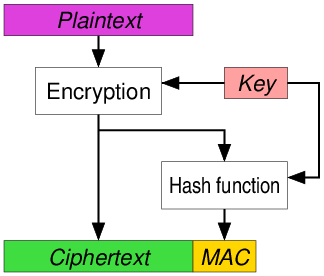
\includegraphics{aeinpractice/aewiki}}}
\fpage{.5}{
\scalebox{0.6}{\Huge
% Graphic for TeX using PGF
% Title: /home/phil/keyreuse.dia
% Creator: Dia v0.97+git
% CreationDate: Fri Mar  8 17:01:06 2019
% For: phil
% \usepackage{tikz}
% The following commands are not supported in PSTricks at present
% We define them conditionally, so when they are implemented,
% this pgf file will use them.
\ifx\du\undefined
  \newlength{\du}
\fi
\setlength{\du}{15\unitlength}
\begin{tikzpicture}[even odd rule]
\pgftransformxscale{1.000000}
\pgftransformyscale{-1.000000}
\definecolor{dialinecolor}{rgb}{0.000000, 0.000000, 0.000000}
\pgfsetstrokecolor{dialinecolor}
\pgfsetstrokeopacity{1.000000}
\definecolor{diafillcolor}{rgb}{1.000000, 1.000000, 1.000000}
\pgfsetfillcolor{diafillcolor}
\pgfsetfillopacity{1.000000}
\pgfsetlinewidth{0.100000\du}
\pgfsetdash{}{0pt}
\pgfsetmiterjoin
{\pgfsetcornersarced{\pgfpoint{0.000000\du}{0.000000\du}}\definecolor{diafillcolor}{rgb}{1.000000, 1.000000, 1.000000}
\pgfsetfillcolor{diafillcolor}
\pgfsetfillopacity{1.000000}
\fill (0.464466\du,12.116117\du)--(0.464466\du,15.566117\du)--(5.464466\du,15.566117\du)--(5.464466\du,12.116117\du)--cycle;
}{\pgfsetcornersarced{\pgfpoint{0.000000\du}{0.000000\du}}\definecolor{dialinecolor}{rgb}{0.000000, 0.000000, 0.000000}
\pgfsetstrokecolor{dialinecolor}
\pgfsetstrokeopacity{1.000000}
\draw (0.464466\du,12.116117\du)--(0.464466\du,15.566117\du)--(5.464466\du,15.566117\du)--(5.464466\du,12.116117\du)--cycle;
}% setfont left to latex
\definecolor{dialinecolor}{rgb}{0.000000, 0.000000, 0.000000}
\pgfsetstrokecolor{dialinecolor}
\pgfsetstrokeopacity{1.000000}
\definecolor{diafillcolor}{rgb}{0.000000, 0.000000, 0.000000}
\pgfsetfillcolor{diafillcolor}
\pgfsetfillopacity{1.000000}
\node[anchor=base,inner sep=0pt, outer sep=0pt,color=dialinecolor] at (2.964466\du,14.185561\du){$E_K$};
% setfont left to latex
\definecolor{dialinecolor}{rgb}{0.000000, 0.000000, 0.000000}
\pgfsetstrokecolor{dialinecolor}
\pgfsetstrokeopacity{1.000000}
\definecolor{diafillcolor}{rgb}{0.000000, 0.000000, 0.000000}
\pgfsetfillcolor{diafillcolor}
\pgfsetfillopacity{1.000000}
\node[anchor=base west,inner sep=0pt,outer sep=0pt,color=dialinecolor] at (2.464466\du,3.116117\du){IV};
\pgfsetlinewidth{0.100000\du}
\pgfsetdash{}{0pt}
\pgfsetmiterjoin
{\pgfsetcornersarced{\pgfpoint{0.000000\du}{0.000000\du}}\definecolor{diafillcolor}{rgb}{1.000000, 1.000000, 1.000000}
\pgfsetfillcolor{diafillcolor}
\pgfsetfillopacity{1.000000}
\fill (7.464466\du,4.116117\du)--(7.464466\du,7.566117\du)--(12.464466\du,7.566117\du)--(12.464466\du,4.116117\du)--cycle;
}{\pgfsetcornersarced{\pgfpoint{0.000000\du}{0.000000\du}}\definecolor{dialinecolor}{rgb}{0.000000, 0.000000, 0.000000}
\pgfsetstrokecolor{dialinecolor}
\pgfsetstrokeopacity{1.000000}
\draw (7.464466\du,4.116117\du)--(7.464466\du,7.566117\du)--(12.464466\du,7.566117\du)--(12.464466\du,4.116117\du)--cycle;
}% setfont left to latex
\definecolor{dialinecolor}{rgb}{0.000000, 0.000000, 0.000000}
\pgfsetstrokecolor{dialinecolor}
\pgfsetstrokeopacity{1.000000}
\definecolor{diafillcolor}{rgb}{0.000000, 0.000000, 0.000000}
\pgfsetfillcolor{diafillcolor}
\pgfsetfillopacity{1.000000}
\node[anchor=base,inner sep=0pt, outer sep=0pt,color=dialinecolor] at (9.964466\du,6.185561\du){$E_K$};
\pgfsetlinewidth{0.100000\du}
\pgfsetdash{}{0pt}
\pgfsetmiterjoin
{\pgfsetcornersarced{\pgfpoint{0.000000\du}{0.000000\du}}\definecolor{diafillcolor}{rgb}{1.000000, 1.000000, 1.000000}
\pgfsetfillcolor{diafillcolor}
\pgfsetfillopacity{1.000000}
\fill (7.464466\du,12.116117\du)--(7.464466\du,15.566117\du)--(12.464466\du,15.566117\du)--(12.464466\du,12.116117\du)--cycle;
}{\pgfsetcornersarced{\pgfpoint{0.000000\du}{0.000000\du}}\definecolor{dialinecolor}{rgb}{0.000000, 0.000000, 0.000000}
\pgfsetstrokecolor{dialinecolor}
\pgfsetstrokeopacity{1.000000}
\draw (7.464466\du,12.116117\du)--(7.464466\du,15.566117\du)--(12.464466\du,15.566117\du)--(12.464466\du,12.116117\du)--cycle;
}% setfont left to latex
\definecolor{dialinecolor}{rgb}{0.000000, 0.000000, 0.000000}
\pgfsetstrokecolor{dialinecolor}
\pgfsetstrokeopacity{1.000000}
\definecolor{diafillcolor}{rgb}{0.000000, 0.000000, 0.000000}
\pgfsetfillcolor{diafillcolor}
\pgfsetfillopacity{1.000000}
\node[anchor=base,inner sep=0pt, outer sep=0pt,color=dialinecolor] at (9.964466\du,14.185561\du){$E_K$};
\pgfsetlinewidth{0.100000\du}
\pgfsetdash{}{0pt}
\pgfsetmiterjoin
{\pgfsetcornersarced{\pgfpoint{0.000000\du}{0.000000\du}}\definecolor{diafillcolor}{rgb}{1.000000, 1.000000, 1.000000}
\pgfsetfillcolor{diafillcolor}
\pgfsetfillopacity{1.000000}
\fill (14.464466\du,4.116117\du)--(14.464466\du,7.566117\du)--(19.464466\du,7.566117\du)--(19.464466\du,4.116117\du)--cycle;
}{\pgfsetcornersarced{\pgfpoint{0.000000\du}{0.000000\du}}\definecolor{dialinecolor}{rgb}{0.000000, 0.000000, 0.000000}
\pgfsetstrokecolor{dialinecolor}
\pgfsetstrokeopacity{1.000000}
\draw (14.464466\du,4.116117\du)--(14.464466\du,7.566117\du)--(19.464466\du,7.566117\du)--(19.464466\du,4.116117\du)--cycle;
}% setfont left to latex
\definecolor{dialinecolor}{rgb}{0.000000, 0.000000, 0.000000}
\pgfsetstrokecolor{dialinecolor}
\pgfsetstrokeopacity{1.000000}
\definecolor{diafillcolor}{rgb}{0.000000, 0.000000, 0.000000}
\pgfsetfillcolor{diafillcolor}
\pgfsetfillopacity{1.000000}
\node[anchor=base,inner sep=0pt, outer sep=0pt,color=dialinecolor] at (16.964466\du,6.185561\du){$E_K$};
\pgfsetlinewidth{0.100000\du}
\pgfsetdash{}{0pt}
\pgfsetmiterjoin
{\pgfsetcornersarced{\pgfpoint{0.000000\du}{0.000000\du}}\definecolor{diafillcolor}{rgb}{1.000000, 1.000000, 1.000000}
\pgfsetfillcolor{diafillcolor}
\pgfsetfillopacity{1.000000}
\fill (14.464466\du,12.116117\du)--(14.464466\du,15.566117\du)--(19.464466\du,15.566117\du)--(19.464466\du,12.116117\du)--cycle;
}{\pgfsetcornersarced{\pgfpoint{0.000000\du}{0.000000\du}}\definecolor{dialinecolor}{rgb}{0.000000, 0.000000, 0.000000}
\pgfsetstrokecolor{dialinecolor}
\pgfsetstrokeopacity{1.000000}
\draw (14.464466\du,12.116117\du)--(14.464466\du,15.566117\du)--(19.464466\du,15.566117\du)--(19.464466\du,12.116117\du)--cycle;
}% setfont left to latex
\definecolor{dialinecolor}{rgb}{0.000000, 0.000000, 0.000000}
\pgfsetstrokecolor{dialinecolor}
\pgfsetstrokeopacity{1.000000}
\definecolor{diafillcolor}{rgb}{0.000000, 0.000000, 0.000000}
\pgfsetfillcolor{diafillcolor}
\pgfsetfillopacity{1.000000}
\node[anchor=base,inner sep=0pt, outer sep=0pt,color=dialinecolor] at (16.964466\du,14.185561\du){$E_K$};
% setfont left to latex
\definecolor{dialinecolor}{rgb}{0.000000, 0.000000, 0.000000}
\pgfsetstrokecolor{dialinecolor}
\pgfsetstrokeopacity{1.000000}
\definecolor{diafillcolor}{rgb}{0.000000, 0.000000, 0.000000}
\pgfsetfillcolor{diafillcolor}
\pgfsetfillopacity{1.000000}
\node[anchor=base west,inner sep=0pt,outer sep=0pt,color=dialinecolor] at (2.464466\du,9.349417\du){$C_0$};
% setfont left to latex
\definecolor{dialinecolor}{rgb}{0.000000, 0.000000, 0.000000}
\pgfsetstrokecolor{dialinecolor}
\pgfsetstrokeopacity{1.000000}
\definecolor{diafillcolor}{rgb}{0.000000, 0.000000, 0.000000}
\pgfsetfillcolor{diafillcolor}
\pgfsetfillopacity{1.000000}
\node[anchor=base west,inner sep=0pt,outer sep=0pt,color=dialinecolor] at (9.464466\du,9.349417\du){$C_1$};
% setfont left to latex
\definecolor{dialinecolor}{rgb}{0.000000, 0.000000, 0.000000}
\pgfsetstrokecolor{dialinecolor}
\pgfsetstrokeopacity{1.000000}
\definecolor{diafillcolor}{rgb}{0.000000, 0.000000, 0.000000}
\pgfsetfillcolor{diafillcolor}
\pgfsetfillopacity{1.000000}
\node[anchor=base west,inner sep=0pt,outer sep=0pt,color=dialinecolor] at (16.464466\du,9.349417\du){$C_2$};
% setfont left to latex
\definecolor{dialinecolor}{rgb}{0.000000, 0.000000, 0.000000}
\pgfsetstrokecolor{dialinecolor}
\pgfsetstrokeopacity{1.000000}
\definecolor{diafillcolor}{rgb}{0.000000, 0.000000, 0.000000}
\pgfsetfillcolor{diafillcolor}
\pgfsetfillopacity{1.000000}
\node[anchor=base west,inner sep=0pt,outer sep=0pt,color=dialinecolor] at (21.464466\du,9.349417\du){T};
\pgfsetlinewidth{0.100000\du}
\pgfsetdash{}{0pt}
\pgfsetbuttcap
{
\definecolor{diafillcolor}{rgb}{0.000000, 0.000000, 0.000000}
\pgfsetfillcolor{diafillcolor}
\pgfsetfillopacity{1.000000}
% was here!!!
\pgfsetarrowsend{stealth}
\definecolor{dialinecolor}{rgb}{0.000000, 0.000000, 0.000000}
\pgfsetstrokecolor{dialinecolor}
\pgfsetstrokeopacity{1.000000}
\draw (2.947796\du,3.666117\du)--(2.931136\du,8.116117\du);
}
\pgfsetlinewidth{0.100000\du}
\pgfsetdash{}{0pt}
\pgfsetbuttcap
{
\definecolor{diafillcolor}{rgb}{0.000000, 0.000000, 0.000000}
\pgfsetfillcolor{diafillcolor}
\pgfsetfillopacity{1.000000}
% was here!!!
\pgfsetarrowsend{stealth}
\definecolor{dialinecolor}{rgb}{0.000000, 0.000000, 0.000000}
\pgfsetstrokecolor{dialinecolor}
\pgfsetstrokeopacity{1.000000}
\draw (9.964466\du,7.566117\du)--(9.864466\du,8.566117\du);
}
\pgfsetlinewidth{0.100000\du}
\pgfsetdash{}{0pt}
\pgfsetbuttcap
{
\definecolor{diafillcolor}{rgb}{0.000000, 0.000000, 0.000000}
\pgfsetfillcolor{diafillcolor}
\pgfsetfillopacity{1.000000}
% was here!!!
\pgfsetarrowsend{stealth}
\definecolor{dialinecolor}{rgb}{0.000000, 0.000000, 0.000000}
\pgfsetstrokecolor{dialinecolor}
\pgfsetstrokeopacity{1.000000}
\draw (16.964466\du,7.566117\du)--(16.914466\du,8.566117\du);
}
\pgfsetlinewidth{0.100000\du}
\pgfsetdash{}{0pt}
\pgfsetbuttcap
{
\definecolor{diafillcolor}{rgb}{0.000000, 0.000000, 0.000000}
\pgfsetfillcolor{diafillcolor}
\pgfsetfillopacity{1.000000}
% was here!!!
\pgfsetarrowsend{stealth}
\definecolor{dialinecolor}{rgb}{0.000000, 0.000000, 0.000000}
\pgfsetstrokecolor{dialinecolor}
\pgfsetstrokeopacity{1.000000}
\draw (2.972796\du,9.499417\du)--(2.964466\du,12.116117\du);
}
\pgfsetlinewidth{0.100000\du}
\pgfsetdash{}{0pt}
\pgfsetbuttcap
\pgfsetmiterjoin
\pgfsetlinewidth{0.100000\du}
\pgfsetbuttcap
\pgfsetmiterjoin
\pgfsetdash{}{0pt}
\definecolor{diafillcolor}{rgb}{1.000000, 1.000000, 1.000000}
\pgfsetfillcolor{diafillcolor}
\pgfsetfillopacity{1.000000}
\pgfpathellipse{\pgfpoint{10.026166\du}{10.801217\du}}{\pgfpoint{0.575000\du}{0\du}}{\pgfpoint{0\du}{0.600000\du}}
\pgfusepath{fill}
\definecolor{dialinecolor}{rgb}{0.000000, 0.000000, 0.000000}
\pgfsetstrokecolor{dialinecolor}
\pgfsetstrokeopacity{1.000000}
\pgfpathellipse{\pgfpoint{10.026166\du}{10.801217\du}}{\pgfpoint{0.575000\du}{0\du}}{\pgfpoint{0\du}{0.600000\du}}
\pgfusepath{stroke}
\pgfsetbuttcap
\pgfsetmiterjoin
\pgfsetdash{}{0pt}
\definecolor{dialinecolor}{rgb}{0.000000, 0.000000, 0.000000}
\pgfsetstrokecolor{dialinecolor}
\pgfsetstrokeopacity{1.000000}
\draw (10.026166\du,10.201217\du)--(10.026166\du,11.401217\du);
\pgfsetbuttcap
\pgfsetmiterjoin
\pgfsetdash{}{0pt}
\definecolor{dialinecolor}{rgb}{0.000000, 0.000000, 0.000000}
\pgfsetstrokecolor{dialinecolor}
\pgfsetstrokeopacity{1.000000}
\draw (9.451166\du,10.801217\du)--(10.601166\du,10.801217\du);
\pgfsetlinewidth{0.100000\du}
\pgfsetdash{}{0pt}
\pgfsetbuttcap
{
\definecolor{diafillcolor}{rgb}{0.000000, 0.000000, 0.000000}
\pgfsetfillcolor{diafillcolor}
\pgfsetfillopacity{1.000000}
% was here!!!
\pgfsetarrowsend{stealth}
\definecolor{dialinecolor}{rgb}{0.000000, 0.000000, 0.000000}
\pgfsetstrokecolor{dialinecolor}
\pgfsetstrokeopacity{1.000000}
\draw (10.034466\du,9.584517\du)--(10.026166\du,10.201217\du);
}
\pgfsetlinewidth{0.100000\du}
\pgfsetdash{}{0pt}
\pgfsetbuttcap
{
\definecolor{diafillcolor}{rgb}{0.000000, 0.000000, 0.000000}
\pgfsetfillcolor{diafillcolor}
\pgfsetfillopacity{1.000000}
% was here!!!
\pgfsetarrowsend{stealth}
\definecolor{dialinecolor}{rgb}{0.000000, 0.000000, 0.000000}
\pgfsetstrokecolor{dialinecolor}
\pgfsetstrokeopacity{1.000000}
\draw (10.026166\du,11.401217\du)--(9.964466\du,12.116117\du);
}
\pgfsetlinewidth{0.100000\du}
\pgfsetdash{}{0pt}
\pgfsetbuttcap
\pgfsetmiterjoin
\pgfsetlinewidth{0.100000\du}
\pgfsetbuttcap
\pgfsetmiterjoin
\pgfsetdash{}{0pt}
\definecolor{diafillcolor}{rgb}{1.000000, 1.000000, 1.000000}
\pgfsetfillcolor{diafillcolor}
\pgfsetfillopacity{1.000000}
\pgfpathellipse{\pgfpoint{16.992766\du}{10.867917\du}}{\pgfpoint{0.575000\du}{0\du}}{\pgfpoint{0\du}{0.600000\du}}
\pgfusepath{fill}
\definecolor{dialinecolor}{rgb}{0.000000, 0.000000, 0.000000}
\pgfsetstrokecolor{dialinecolor}
\pgfsetstrokeopacity{1.000000}
\pgfpathellipse{\pgfpoint{16.992766\du}{10.867917\du}}{\pgfpoint{0.575000\du}{0\du}}{\pgfpoint{0\du}{0.600000\du}}
\pgfusepath{stroke}
\pgfsetbuttcap
\pgfsetmiterjoin
\pgfsetdash{}{0pt}
\definecolor{dialinecolor}{rgb}{0.000000, 0.000000, 0.000000}
\pgfsetstrokecolor{dialinecolor}
\pgfsetstrokeopacity{1.000000}
\draw (16.992766\du,10.267917\du)--(16.992766\du,11.467917\du);
\pgfsetbuttcap
\pgfsetmiterjoin
\pgfsetdash{}{0pt}
\definecolor{dialinecolor}{rgb}{0.000000, 0.000000, 0.000000}
\pgfsetstrokecolor{dialinecolor}
\pgfsetstrokeopacity{1.000000}
\draw (16.417766\du,10.867917\du)--(17.567766\du,10.867917\du);
\pgfsetlinewidth{0.100000\du}
\pgfsetdash{}{0pt}
\pgfsetbuttcap
{
\definecolor{diafillcolor}{rgb}{0.000000, 0.000000, 0.000000}
\pgfsetfillcolor{diafillcolor}
\pgfsetfillopacity{1.000000}
% was here!!!
\pgfsetarrowsend{stealth}
\definecolor{dialinecolor}{rgb}{0.000000, 0.000000, 0.000000}
\pgfsetstrokecolor{dialinecolor}
\pgfsetstrokeopacity{1.000000}
\draw (17.001166\du,9.651217\du)--(16.992766\du,10.267917\du);
}
\pgfsetlinewidth{0.100000\du}
\pgfsetdash{}{0pt}
\pgfsetbuttcap
{
\definecolor{diafillcolor}{rgb}{0.000000, 0.000000, 0.000000}
\pgfsetfillcolor{diafillcolor}
\pgfsetfillopacity{1.000000}
% was here!!!
\pgfsetarrowsend{stealth}
\definecolor{dialinecolor}{rgb}{0.000000, 0.000000, 0.000000}
\pgfsetstrokecolor{dialinecolor}
\pgfsetstrokeopacity{1.000000}
\draw (16.992766\du,11.467917\du)--(16.964466\du,12.116117\du);
}
\pgfsetlinewidth{0.100000\du}
\pgfsetdash{}{0pt}
\pgfsetmiterjoin
\pgfsetbuttcap
{
\definecolor{diafillcolor}{rgb}{0.000000, 0.000000, 0.000000}
\pgfsetfillcolor{diafillcolor}
\pgfsetfillopacity{1.000000}
% was here!!!
\pgfsetarrowsend{stealth}
{\pgfsetcornersarced{\pgfpoint{0.000000\du}{0.000000\du}}\definecolor{dialinecolor}{rgb}{0.000000, 0.000000, 0.000000}
\pgfsetstrokecolor{dialinecolor}
\pgfsetstrokeopacity{1.000000}
\draw (2.964466\du,15.566117\du)--(2.964466\du,16.616117\du)--(6.182816\du,16.616117\du)--(6.182816\du,10.801217\du)--(9.451166\du,10.801217\du);
}}
\pgfsetlinewidth{0.100000\du}
\pgfsetdash{}{0pt}
\pgfsetbuttcap
{
\definecolor{diafillcolor}{rgb}{0.000000, 0.000000, 0.000000}
\pgfsetfillcolor{diafillcolor}
\pgfsetfillopacity{1.000000}
% was here!!!
\pgfsetarrowsend{stealth}
\definecolor{dialinecolor}{rgb}{0.000000, 0.000000, 0.000000}
\pgfsetstrokecolor{dialinecolor}
\pgfsetstrokeopacity{1.000000}
\draw (3.747796\du,2.699447\du)--(9.451166\du,2.791217\du);
}
\pgfsetlinewidth{0.100000\du}
\pgfsetdash{}{0pt}
\pgfsetmiterjoin
\pgfsetbuttcap
{
\definecolor{diafillcolor}{rgb}{0.000000, 0.000000, 0.000000}
\pgfsetfillcolor{diafillcolor}
\pgfsetfillopacity{1.000000}
% was here!!!
\pgfsetarrowsend{stealth}
{\pgfsetcornersarced{\pgfpoint{0.000000\du}{0.000000\du}}\definecolor{dialinecolor}{rgb}{0.000000, 0.000000, 0.000000}
\pgfsetstrokecolor{dialinecolor}
\pgfsetstrokeopacity{1.000000}
\draw (9.964466\du,15.566117\du)--(9.964466\du,16.616117\du)--(13.166116\du,16.616117\du)--(13.166116\du,10.867917\du)--(16.417766\du,10.867917\du);
}}
\pgfsetlinewidth{0.100000\du}
\pgfsetdash{}{0pt}
\pgfsetmiterjoin
\pgfsetbuttcap
{
\definecolor{diafillcolor}{rgb}{0.000000, 0.000000, 0.000000}
\pgfsetfillcolor{diafillcolor}
\pgfsetfillopacity{1.000000}
% was here!!!
\pgfsetarrowsend{stealth}
{\pgfsetcornersarced{\pgfpoint{0.000000\du}{0.000000\du}}\definecolor{dialinecolor}{rgb}{0.000000, 0.000000, 0.000000}
\pgfsetstrokecolor{dialinecolor}
\pgfsetstrokeopacity{1.000000}
\draw (16.964466\du,15.566117\du)--(16.964466\du,16.616117\du)--(20.381166\du,16.616117\du)--(20.381166\du,8.982787\du)--(21.481166\du,8.982787\du);
}}
% setfont left to latex
\definecolor{dialinecolor}{rgb}{0.000000, 0.000000, 0.000000}
\pgfsetstrokecolor{dialinecolor}
\pgfsetstrokeopacity{1.000000}
\definecolor{diafillcolor}{rgb}{0.000000, 0.000000, 0.000000}
\pgfsetfillcolor{diafillcolor}
\pgfsetfillopacity{1.000000}
\node[anchor=base west,inner sep=0pt,outer sep=0pt,color=dialinecolor] at (9.464466\du,1.339447\du){$M_1$};
\pgfsetlinewidth{0.100000\du}
\pgfsetdash{}{0pt}
\pgfsetbuttcap
\pgfsetmiterjoin
\pgfsetlinewidth{0.100000\du}
\pgfsetbuttcap
\pgfsetmiterjoin
\pgfsetdash{}{0pt}
\definecolor{diafillcolor}{rgb}{1.000000, 1.000000, 1.000000}
\pgfsetfillcolor{diafillcolor}
\pgfsetfillopacity{1.000000}
\pgfpathellipse{\pgfpoint{10.026166\du}{2.791217\du}}{\pgfpoint{0.575000\du}{0\du}}{\pgfpoint{0\du}{0.600000\du}}
\pgfusepath{fill}
\definecolor{dialinecolor}{rgb}{0.000000, 0.000000, 0.000000}
\pgfsetstrokecolor{dialinecolor}
\pgfsetstrokeopacity{1.000000}
\pgfpathellipse{\pgfpoint{10.026166\du}{2.791217\du}}{\pgfpoint{0.575000\du}{0\du}}{\pgfpoint{0\du}{0.600000\du}}
\pgfusepath{stroke}
\pgfsetbuttcap
\pgfsetmiterjoin
\pgfsetdash{}{0pt}
\definecolor{dialinecolor}{rgb}{0.000000, 0.000000, 0.000000}
\pgfsetstrokecolor{dialinecolor}
\pgfsetstrokeopacity{1.000000}
\draw (10.026166\du,2.191217\du)--(10.026166\du,3.391217\du);
\pgfsetbuttcap
\pgfsetmiterjoin
\pgfsetdash{}{0pt}
\definecolor{dialinecolor}{rgb}{0.000000, 0.000000, 0.000000}
\pgfsetstrokecolor{dialinecolor}
\pgfsetstrokeopacity{1.000000}
\draw (9.451166\du,2.791217\du)--(10.601166\du,2.791217\du);
\pgfsetlinewidth{0.100000\du}
\pgfsetdash{}{0pt}
\pgfsetbuttcap
{
\definecolor{diafillcolor}{rgb}{0.000000, 0.000000, 0.000000}
\pgfsetfillcolor{diafillcolor}
\pgfsetfillopacity{1.000000}
% was here!!!
\pgfsetarrowsend{stealth}
\definecolor{dialinecolor}{rgb}{0.000000, 0.000000, 0.000000}
\pgfsetstrokecolor{dialinecolor}
\pgfsetstrokeopacity{1.000000}
\draw (10.034466\du,1.574547\du)--(10.026166\du,2.191217\du);
}
\pgfsetlinewidth{0.100000\du}
\pgfsetdash{}{0pt}
\pgfsetbuttcap
{
\definecolor{diafillcolor}{rgb}{0.000000, 0.000000, 0.000000}
\pgfsetfillcolor{diafillcolor}
\pgfsetfillopacity{1.000000}
% was here!!!
\pgfsetarrowsend{stealth}
\definecolor{dialinecolor}{rgb}{0.000000, 0.000000, 0.000000}
\pgfsetstrokecolor{dialinecolor}
\pgfsetstrokeopacity{1.000000}
\draw (10.026166\du,3.391217\du)--(9.964466\du,4.116117\du);
}
% setfont left to latex
\definecolor{dialinecolor}{rgb}{0.000000, 0.000000, 0.000000}
\pgfsetstrokecolor{dialinecolor}
\pgfsetstrokeopacity{1.000000}
\definecolor{diafillcolor}{rgb}{0.000000, 0.000000, 0.000000}
\pgfsetfillcolor{diafillcolor}
\pgfsetfillopacity{1.000000}
\node[anchor=base west,inner sep=0pt,outer sep=0pt,color=dialinecolor] at (16.434466\du,1.279447\du){$M_2$};
\pgfsetlinewidth{0.100000\du}
\pgfsetdash{}{0pt}
\pgfsetbuttcap
\pgfsetmiterjoin
\pgfsetlinewidth{0.100000\du}
\pgfsetbuttcap
\pgfsetmiterjoin
\pgfsetdash{}{0pt}
\definecolor{diafillcolor}{rgb}{1.000000, 1.000000, 1.000000}
\pgfsetfillcolor{diafillcolor}
\pgfsetfillopacity{1.000000}
\pgfpathellipse{\pgfpoint{16.996166\du}{2.731217\du}}{\pgfpoint{0.575000\du}{0\du}}{\pgfpoint{0\du}{0.600000\du}}
\pgfusepath{fill}
\definecolor{dialinecolor}{rgb}{0.000000, 0.000000, 0.000000}
\pgfsetstrokecolor{dialinecolor}
\pgfsetstrokeopacity{1.000000}
\pgfpathellipse{\pgfpoint{16.996166\du}{2.731217\du}}{\pgfpoint{0.575000\du}{0\du}}{\pgfpoint{0\du}{0.600000\du}}
\pgfusepath{stroke}
\pgfsetbuttcap
\pgfsetmiterjoin
\pgfsetdash{}{0pt}
\definecolor{dialinecolor}{rgb}{0.000000, 0.000000, 0.000000}
\pgfsetstrokecolor{dialinecolor}
\pgfsetstrokeopacity{1.000000}
\draw (16.996166\du,2.131217\du)--(16.996166\du,3.331217\du);
\pgfsetbuttcap
\pgfsetmiterjoin
\pgfsetdash{}{0pt}
\definecolor{dialinecolor}{rgb}{0.000000, 0.000000, 0.000000}
\pgfsetstrokecolor{dialinecolor}
\pgfsetstrokeopacity{1.000000}
\draw (16.421166\du,2.731217\du)--(17.571166\du,2.731217\du);
\pgfsetlinewidth{0.100000\du}
\pgfsetdash{}{0pt}
\pgfsetbuttcap
{
\definecolor{diafillcolor}{rgb}{0.000000, 0.000000, 0.000000}
\pgfsetfillcolor{diafillcolor}
\pgfsetfillopacity{1.000000}
% was here!!!
\pgfsetarrowsend{stealth}
\definecolor{dialinecolor}{rgb}{0.000000, 0.000000, 0.000000}
\pgfsetstrokecolor{dialinecolor}
\pgfsetstrokeopacity{1.000000}
\draw (17.004466\du,1.514547\du)--(16.996166\du,2.131217\du);
}
\pgfsetlinewidth{0.100000\du}
\pgfsetdash{}{0pt}
\pgfsetbuttcap
{
\definecolor{diafillcolor}{rgb}{0.000000, 0.000000, 0.000000}
\pgfsetfillcolor{diafillcolor}
\pgfsetfillopacity{1.000000}
% was here!!!
\pgfsetarrowsend{stealth}
\definecolor{dialinecolor}{rgb}{0.000000, 0.000000, 0.000000}
\pgfsetstrokecolor{dialinecolor}
\pgfsetstrokeopacity{1.000000}
\draw (16.996166\du,3.331217\du)--(16.964466\du,4.116117\du);
}
\pgfsetlinewidth{0.100000\du}
\pgfsetdash{}{0pt}
\pgfsetmiterjoin
\pgfsetbuttcap
{
\definecolor{diafillcolor}{rgb}{0.000000, 0.000000, 0.000000}
\pgfsetfillcolor{diafillcolor}
\pgfsetfillopacity{1.000000}
% was here!!!
\pgfsetarrowsend{stealth}
{\pgfsetcornersarced{\pgfpoint{0.000000\du}{0.000000\du}}\definecolor{dialinecolor}{rgb}{0.000000, 0.000000, 0.000000}
\pgfsetstrokecolor{dialinecolor}
\pgfsetstrokeopacity{1.000000}
\draw (11.068759\du,9.016117\du)--(13.744962\du,9.016117\du)--(13.744962\du,2.731217\du)--(16.421166\du,2.731217\du);
}}
\end{tikzpicture}
\normalsize}}
  \caption{One encryption scheme that reuses keys across MAC and encryption primitives (right), as suggested in this diagram from Wikipedia (left)}
\label{fig:reusescheme}
\end{figure}

Consider the right side of Figure~\ref{fig:reusescheme}.  This shows one example construction, composing CBC-Mode+CBC-MAC using an encrypt-then-MAC 
paradigm where the ciphertexts are MACd, as suggested by AE-WIKI.  We concretely instantiate the scheme with messages consisting of two blocks, but 
consider the generalization to $n$ blocks by the obvious changes to the above structure.

While CBC mode provides the security we require, an adversary can easily violate ROR+CTXT for this scheme.  Remember the definition of the CTXT game 
in the previous chapter; an adversary must forge a ciphertext not returned by the encryption oracle, that decrypts without throwing an error.

To do so, consider a CTXT adversary $A$, whose operation is illustrated in Figure~\ref{fig:reuseadversary}.  First, the adversary queries the 
encryption of $0^n$, as shown on the left, so $C_0C_1T \leftarrow Enc(0^n)$.  The adversarially controlled inputs are shown with a red box surrounding 
them.

Next, the adversary calls $R \leftarrow Dec(0^nTT)$.  We will now show that $R \neq \bot$ with probability $1-\frac{1}{2^n}$, and therefore $A$ wins 
the CTXT game with this probability.


\begin{figure}
\centering
\scalebox{0.6}{% Graphic for TeX using PGF
% Title: /home/phil/keyreuse3.dia
% Creator: Dia v0.97+git
% CreationDate: Fri Mar  8 13:42:53 2019
% For: phil
% \usepackage{tikz}
% The following commands are not supported in PSTricks at present
% We define them conditionally, so when they are implemented,
% this pgf file will use them.
\Huge
\ifx\du\undefined
  \newlength{\du}
\fi
\setlength{\du}{15\unitlength}
\begin{tikzpicture}[even odd rule]
\pgftransformxscale{1.000000}
\pgftransformyscale{-1.000000}
\definecolor{dialinecolor}{rgb}{0.000000, 0.000000, 0.000000}
\pgfsetstrokecolor{dialinecolor}
\pgfsetstrokeopacity{1.000000}
\definecolor{diafillcolor}{rgb}{1.000000, 1.000000, 1.000000}
\pgfsetfillcolor{diafillcolor}
\pgfsetfillopacity{1.000000}
\pgfsetlinewidth{0.100000\du}
\pgfsetdash{}{0pt}
\pgfsetmiterjoin
{\pgfsetcornersarced{\pgfpoint{0.000000\du}{0.000000\du}}\definecolor{diafillcolor}{rgb}{1.000000, 0.000000, 0.000000}
\pgfsetfillcolor{diafillcolor}
\pgfsetfillopacity{1.000000}
\fill (24.300000\du,9.500000\du)--(24.300000\du,11.950000\du)--(42.300000\du,11.950000\du)--(42.300000\du,9.500000\du)--cycle;
}{\pgfsetcornersarced{\pgfpoint{0.000000\du}{0.000000\du}}\definecolor{dialinecolor}{rgb}{0.000000, 0.000000, 0.000000}
\pgfsetstrokecolor{dialinecolor}
\pgfsetstrokeopacity{1.000000}
\draw (24.300000\du,9.500000\du)--(24.300000\du,11.950000\du)--(42.300000\du,11.950000\du)--(42.300000\du,9.500000\du)--cycle;
}% setfont left to latex
\definecolor{dialinecolor}{rgb}{0.000000, 0.000000, 0.000000}
\pgfsetstrokecolor{dialinecolor}
\pgfsetstrokeopacity{1.000000}
\definecolor{diafillcolor}{rgb}{0.000000, 0.000000, 0.000000}
\pgfsetfillcolor{diafillcolor}
\pgfsetfillopacity{1.000000}
\node[anchor=base,inner sep=0pt, outer sep=0pt,color=dialinecolor] at (33.300000\du,10.920000\du){};
\pgfsetlinewidth{0.100000\du}
\pgfsetdash{}{0pt}
\pgfsetmiterjoin
{\pgfsetcornersarced{\pgfpoint{0.000000\du}{0.000000\du}}\definecolor{diafillcolor}{rgb}{1.000000, 1.000000, 1.000000}
\pgfsetfillcolor{diafillcolor}
\pgfsetfillopacity{1.000000}
\fill (23.200000\du,13.733333\du)--(23.200000\du,17.183333\du)--(28.200000\du,17.183333\du)--(28.200000\du,13.733333\du)--cycle;
}{\pgfsetcornersarced{\pgfpoint{0.000000\du}{0.000000\du}}\definecolor{dialinecolor}{rgb}{0.000000, 0.000000, 0.000000}
\pgfsetstrokecolor{dialinecolor}
\pgfsetstrokeopacity{1.000000}
\draw (23.200000\du,13.733333\du)--(23.200000\du,17.183333\du)--(28.200000\du,17.183333\du)--(28.200000\du,13.733333\du)--cycle;
}% setfont left to latex
\definecolor{dialinecolor}{rgb}{0.000000, 0.000000, 0.000000}
\pgfsetstrokecolor{dialinecolor}
\pgfsetstrokeopacity{1.000000}
\definecolor{diafillcolor}{rgb}{0.000000, 0.000000, 0.000000}
\pgfsetfillcolor{diafillcolor}
\pgfsetfillopacity{1.000000}
\node[anchor=base,inner sep=0pt, outer sep=0pt,color=dialinecolor] at (25.700000\du,15.802778\du){$E_k$};
% setfont left to latex
\definecolor{dialinecolor}{rgb}{0.000000, 0.000000, 0.000000}
\pgfsetstrokecolor{dialinecolor}
\pgfsetstrokeopacity{1.000000}
\definecolor{diafillcolor}{rgb}{0.000000, 0.000000, 0.000000}
\pgfsetfillcolor{diafillcolor}
\pgfsetfillopacity{1.000000}
\node[anchor=base west,inner sep=0pt,outer sep=0pt,color=dialinecolor] at (25.200000\du,4.733333\du){IV};
\pgfsetlinewidth{0.100000\du}
\pgfsetdash{}{0pt}
\pgfsetmiterjoin
{\pgfsetcornersarced{\pgfpoint{0.000000\du}{0.000000\du}}\definecolor{diafillcolor}{rgb}{1.000000, 1.000000, 1.000000}
\pgfsetfillcolor{diafillcolor}
\pgfsetfillopacity{1.000000}
\fill (30.300000\du,5.733333\du)--(30.300000\du,9.183333\du)--(35.300000\du,9.183333\du)--(35.300000\du,5.733333\du)--cycle;
}{\pgfsetcornersarced{\pgfpoint{0.000000\du}{0.000000\du}}\definecolor{dialinecolor}{rgb}{0.000000, 0.000000, 0.000000}
\pgfsetstrokecolor{dialinecolor}
\pgfsetstrokeopacity{1.000000}
\draw (30.300000\du,5.733333\du)--(30.300000\du,9.183333\du)--(35.300000\du,9.183333\du)--(35.300000\du,5.733333\du)--cycle;
}% setfont left to latex
\definecolor{dialinecolor}{rgb}{0.000000, 0.000000, 0.000000}
\pgfsetstrokecolor{dialinecolor}
\pgfsetstrokeopacity{1.000000}
\definecolor{diafillcolor}{rgb}{0.000000, 0.000000, 0.000000}
\pgfsetfillcolor{diafillcolor}
\pgfsetfillopacity{1.000000}
\node[anchor=base,inner sep=0pt, outer sep=0pt,color=dialinecolor] at (32.800000\du,7.802778\du){$E_K$};
\pgfsetlinewidth{0.100000\du}
\pgfsetdash{}{0pt}
\pgfsetmiterjoin
{\pgfsetcornersarced{\pgfpoint{0.000000\du}{0.000000\du}}\definecolor{diafillcolor}{rgb}{1.000000, 1.000000, 1.000000}
\pgfsetfillcolor{diafillcolor}
\pgfsetfillopacity{1.000000}
\fill (30.300000\du,13.733333\du)--(30.300000\du,17.183333\du)--(35.300000\du,17.183333\du)--(35.300000\du,13.733333\du)--cycle;
}{\pgfsetcornersarced{\pgfpoint{0.000000\du}{0.000000\du}}\definecolor{dialinecolor}{rgb}{0.000000, 0.000000, 0.000000}
\pgfsetstrokecolor{dialinecolor}
\pgfsetstrokeopacity{1.000000}
\draw (30.300000\du,13.733333\du)--(30.300000\du,17.183333\du)--(35.300000\du,17.183333\du)--(35.300000\du,13.733333\du)--cycle;
}% setfont left to latex
\definecolor{dialinecolor}{rgb}{0.000000, 0.000000, 0.000000}
\pgfsetstrokecolor{dialinecolor}
\pgfsetstrokeopacity{1.000000}
\definecolor{diafillcolor}{rgb}{0.000000, 0.000000, 0.000000}
\pgfsetfillcolor{diafillcolor}
\pgfsetfillopacity{1.000000}
\node[anchor=base,inner sep=0pt, outer sep=0pt,color=dialinecolor] at (32.800000\du,15.802778\du){$E_k$};
% setfont left to latex
\definecolor{dialinecolor}{rgb}{0.000000, 0.000000, 0.000000}
\pgfsetstrokecolor{dialinecolor}
\pgfsetstrokeopacity{1.000000}
\definecolor{diafillcolor}{rgb}{0.000000, 0.000000, 0.000000}
\pgfsetfillcolor{diafillcolor}
\pgfsetfillopacity{1.000000}
\node[anchor=base west,inner sep=0pt,outer sep=0pt,color=dialinecolor] at (25.300000\du,10.966667\du){$0^n$};
% setfont left to latex
\definecolor{dialinecolor}{rgb}{0.000000, 0.000000, 0.000000}
\pgfsetstrokecolor{dialinecolor}
\pgfsetstrokeopacity{1.000000}
\definecolor{diafillcolor}{rgb}{0.000000, 0.000000, 0.000000}
\pgfsetfillcolor{diafillcolor}
\pgfsetfillopacity{1.000000}
\node[anchor=base west,inner sep=0pt,outer sep=0pt,color=dialinecolor] at (32.433333\du,11.033333\du){T};
% setfont left to latex
\definecolor{dialinecolor}{rgb}{0.000000, 0.000000, 0.000000}
\pgfsetstrokecolor{dialinecolor}
\pgfsetstrokeopacity{1.000000}
\definecolor{diafillcolor}{rgb}{0.000000, 0.000000, 0.000000}
\pgfsetfillcolor{diafillcolor}
\pgfsetfillopacity{1.000000}
\node[anchor=base west,inner sep=0pt,outer sep=0pt,color=dialinecolor] at (37.300000\du,10.966667\du){$E_K(0^n)$};
\pgfsetlinewidth{0.100000\du}
\pgfsetdash{}{0pt}
\pgfsetbuttcap
{
\definecolor{diafillcolor}{rgb}{0.000000, 0.000000, 0.000000}
\pgfsetfillcolor{diafillcolor}
\pgfsetfillopacity{1.000000}
% was here!!!
\pgfsetarrowsend{stealth}
\definecolor{dialinecolor}{rgb}{0.000000, 0.000000, 0.000000}
\pgfsetstrokecolor{dialinecolor}
\pgfsetstrokeopacity{1.000000}
\draw (25.683333\du,5.283333\du)--(25.666667\du,9.733333\du);
}
\pgfsetlinewidth{0.100000\du}
\pgfsetdash{}{0pt}
\pgfsetbuttcap
{
\definecolor{diafillcolor}{rgb}{0.000000, 0.000000, 0.000000}
\pgfsetfillcolor{diafillcolor}
\pgfsetfillopacity{1.000000}
% was here!!!
\pgfsetarrowsend{stealth}
\definecolor{dialinecolor}{rgb}{0.000000, 0.000000, 0.000000}
\pgfsetstrokecolor{dialinecolor}
\pgfsetstrokeopacity{1.000000}
\draw (32.800000\du,9.183333\du)--(32.750000\du,10.183333\du);
}
\pgfsetlinewidth{0.100000\du}
\pgfsetdash{}{0pt}
\pgfsetbuttcap
{
\definecolor{diafillcolor}{rgb}{0.000000, 0.000000, 0.000000}
\pgfsetfillcolor{diafillcolor}
\pgfsetfillopacity{1.000000}
% was here!!!
\pgfsetarrowsend{stealth}
\definecolor{dialinecolor}{rgb}{0.000000, 0.000000, 0.000000}
\pgfsetstrokecolor{dialinecolor}
\pgfsetstrokeopacity{1.000000}
\draw (25.708333\du,11.116667\du)--(25.700000\du,13.733333\du);
}
\pgfsetlinewidth{0.100000\du}
\pgfsetdash{}{0pt}
\pgfsetbuttcap
\pgfsetmiterjoin
\pgfsetlinewidth{0.100000\du}
\pgfsetbuttcap
\pgfsetmiterjoin
\pgfsetdash{}{0pt}
\definecolor{diafillcolor}{rgb}{1.000000, 1.000000, 1.000000}
\pgfsetfillcolor{diafillcolor}
\pgfsetfillopacity{1.000000}
\pgfpathellipse{\pgfpoint{32.828333\du}{12.485096\du}}{\pgfpoint{0.575000\du}{0\du}}{\pgfpoint{0\du}{0.600000\du}}
\pgfusepath{fill}
\definecolor{dialinecolor}{rgb}{0.000000, 0.000000, 0.000000}
\pgfsetstrokecolor{dialinecolor}
\pgfsetstrokeopacity{1.000000}
\pgfpathellipse{\pgfpoint{32.828333\du}{12.485096\du}}{\pgfpoint{0.575000\du}{0\du}}{\pgfpoint{0\du}{0.600000\du}}
\pgfusepath{stroke}
\pgfsetbuttcap
\pgfsetmiterjoin
\pgfsetdash{}{0pt}
\definecolor{dialinecolor}{rgb}{0.000000, 0.000000, 0.000000}
\pgfsetstrokecolor{dialinecolor}
\pgfsetstrokeopacity{1.000000}
\draw (32.828333\du,11.885096\du)--(32.828333\du,13.085096\du);
\pgfsetbuttcap
\pgfsetmiterjoin
\pgfsetdash{}{0pt}
\definecolor{dialinecolor}{rgb}{0.000000, 0.000000, 0.000000}
\pgfsetstrokecolor{dialinecolor}
\pgfsetstrokeopacity{1.000000}
\draw (32.253333\du,12.485096\du)--(33.403333\du,12.485096\du);
\pgfsetlinewidth{0.100000\du}
\pgfsetdash{}{0pt}
\pgfsetbuttcap
{
\definecolor{diafillcolor}{rgb}{0.000000, 0.000000, 0.000000}
\pgfsetfillcolor{diafillcolor}
\pgfsetfillopacity{1.000000}
% was here!!!
\pgfsetarrowsend{stealth}
\definecolor{dialinecolor}{rgb}{0.000000, 0.000000, 0.000000}
\pgfsetstrokecolor{dialinecolor}
\pgfsetstrokeopacity{1.000000}
\draw (32.836667\du,11.268430\du)--(32.828333\du,11.885096\du);
}
\pgfsetlinewidth{0.100000\du}
\pgfsetdash{}{0pt}
\pgfsetbuttcap
{
\definecolor{diafillcolor}{rgb}{0.000000, 0.000000, 0.000000}
\pgfsetfillcolor{diafillcolor}
\pgfsetfillopacity{1.000000}
% was here!!!
\pgfsetarrowsend{stealth}
\definecolor{dialinecolor}{rgb}{0.000000, 0.000000, 0.000000}
\pgfsetstrokecolor{dialinecolor}
\pgfsetstrokeopacity{1.000000}
\draw (32.828333\du,13.085096\du)--(32.800000\du,13.733333\du);
}
\pgfsetlinewidth{0.100000\du}
\pgfsetdash{}{0pt}
\pgfsetmiterjoin
\pgfsetbuttcap
{
\definecolor{diafillcolor}{rgb}{0.000000, 0.000000, 0.000000}
\pgfsetfillcolor{diafillcolor}
\pgfsetfillopacity{1.000000}
% was here!!!
\pgfsetarrowsend{stealth}
{\pgfsetcornersarced{\pgfpoint{0.000000\du}{0.000000\du}}\definecolor{dialinecolor}{rgb}{0.000000, 0.000000, 0.000000}
\pgfsetstrokecolor{dialinecolor}
\pgfsetstrokeopacity{1.000000}
\draw (25.700000\du,17.183333\du)--(25.700000\du,18.233333\du)--(28.951667\du,18.233333\du)--(28.951667\du,12.485096\du)--(32.253333\du,12.485096\du);
}}
\pgfsetlinewidth{0.100000\du}
\pgfsetdash{}{0pt}
\pgfsetbuttcap
{
\definecolor{diafillcolor}{rgb}{0.000000, 0.000000, 0.000000}
\pgfsetfillcolor{diafillcolor}
\pgfsetfillopacity{1.000000}
% was here!!!
\pgfsetarrowsend{stealth}
\definecolor{dialinecolor}{rgb}{0.000000, 0.000000, 0.000000}
\pgfsetstrokecolor{dialinecolor}
\pgfsetstrokeopacity{1.000000}
\draw (26.483333\du,4.316667\du)--(32.256667\du,4.348430\du);
}
\pgfsetlinewidth{0.100000\du}
\pgfsetdash{}{0pt}
\pgfsetmiterjoin
\pgfsetbuttcap
{
\definecolor{diafillcolor}{rgb}{0.000000, 0.000000, 0.000000}
\pgfsetfillcolor{diafillcolor}
\pgfsetfillopacity{1.000000}
% was here!!!
\pgfsetarrowsend{stealth}
{\pgfsetcornersarced{\pgfpoint{0.000000\du}{0.000000\du}}\definecolor{dialinecolor}{rgb}{0.000000, 0.000000, 0.000000}
\pgfsetstrokecolor{dialinecolor}
\pgfsetstrokeopacity{1.000000}
\draw (32.800000\du,17.183333\du)--(32.800000\du,18.233333\du)--(36.216667\du,18.233333\du)--(36.216667\du,10.600000\du)--(37.316667\du,10.600000\du);
}}
% setfont left to latex
\definecolor{dialinecolor}{rgb}{0.000000, 0.000000, 0.000000}
\pgfsetstrokecolor{dialinecolor}
\pgfsetstrokeopacity{1.000000}
\definecolor{diafillcolor}{rgb}{0.000000, 0.000000, 0.000000}
\pgfsetfillcolor{diafillcolor}
\pgfsetfillopacity{1.000000}
\node[anchor=base west,inner sep=0pt,outer sep=0pt,color=dialinecolor] at (32.070000\du,2.596667\du){$0^n$};
\pgfsetlinewidth{0.100000\du}
\pgfsetdash{}{0pt}
\pgfsetbuttcap
\pgfsetmiterjoin
\pgfsetlinewidth{0.100000\du}
\pgfsetbuttcap
\pgfsetmiterjoin
\pgfsetdash{}{0pt}
\definecolor{diafillcolor}{rgb}{1.000000, 1.000000, 1.000000}
\pgfsetfillcolor{diafillcolor}
\pgfsetfillopacity{1.000000}
\pgfpathellipse{\pgfpoint{32.831667\du}{4.348430\du}}{\pgfpoint{0.575000\du}{0\du}}{\pgfpoint{0\du}{0.600000\du}}
\pgfusepath{fill}
\definecolor{dialinecolor}{rgb}{0.000000, 0.000000, 0.000000}
\pgfsetstrokecolor{dialinecolor}
\pgfsetstrokeopacity{1.000000}
\pgfpathellipse{\pgfpoint{32.831667\du}{4.348430\du}}{\pgfpoint{0.575000\du}{0\du}}{\pgfpoint{0\du}{0.600000\du}}
\pgfusepath{stroke}
\pgfsetbuttcap
\pgfsetmiterjoin
\pgfsetdash{}{0pt}
\definecolor{dialinecolor}{rgb}{0.000000, 0.000000, 0.000000}
\pgfsetstrokecolor{dialinecolor}
\pgfsetstrokeopacity{1.000000}
\draw (32.831667\du,3.748430\du)--(32.831667\du,4.948430\du);
\pgfsetbuttcap
\pgfsetmiterjoin
\pgfsetdash{}{0pt}
\definecolor{dialinecolor}{rgb}{0.000000, 0.000000, 0.000000}
\pgfsetstrokecolor{dialinecolor}
\pgfsetstrokeopacity{1.000000}
\draw (32.256667\du,4.348430\du)--(33.406667\du,4.348430\du);
\pgfsetlinewidth{0.100000\du}
\pgfsetdash{}{0pt}
\pgfsetbuttcap
{
\definecolor{diafillcolor}{rgb}{0.000000, 0.000000, 0.000000}
\pgfsetfillcolor{diafillcolor}
\pgfsetfillopacity{1.000000}
% was here!!!
\pgfsetarrowsend{stealth}
\definecolor{dialinecolor}{rgb}{0.000000, 0.000000, 0.000000}
\pgfsetstrokecolor{dialinecolor}
\pgfsetstrokeopacity{1.000000}
\draw (32.840000\du,3.131763\du)--(32.831667\du,3.748430\du);
}
\pgfsetlinewidth{0.100000\du}
\pgfsetdash{}{0pt}
\pgfsetbuttcap
{
\definecolor{diafillcolor}{rgb}{0.000000, 0.000000, 0.000000}
\pgfsetfillcolor{diafillcolor}
\pgfsetfillopacity{1.000000}
% was here!!!
\pgfsetarrowsend{stealth}
\definecolor{dialinecolor}{rgb}{0.000000, 0.000000, 0.000000}
\pgfsetstrokecolor{dialinecolor}
\pgfsetstrokeopacity{1.000000}
\draw (32.831667\du,4.948430\du)--(32.800000\du,5.733333\du);
}
% setfont left to latex
\definecolor{dialinecolor}{rgb}{0.000000, 0.000000, 0.000000}
\pgfsetstrokecolor{dialinecolor}
\pgfsetstrokeopacity{1.000000}
\definecolor{diafillcolor}{rgb}{0.000000, 0.000000, 0.000000}
\pgfsetfillcolor{diafillcolor}
\pgfsetfillopacity{1.000000}
\node[anchor=base west,inner sep=0pt,outer sep=0pt,color=dialinecolor] at (32.841667\du,10.650000\du){};
% setfont left to latex
\definecolor{dialinecolor}{rgb}{0.000000, 0.000000, 0.000000}
\pgfsetstrokecolor{dialinecolor}
\pgfsetstrokeopacity{1.000000}
\definecolor{diafillcolor}{rgb}{0.000000, 0.000000, 0.000000}
\pgfsetfillcolor{diafillcolor}
\pgfsetfillopacity{1.000000}
\node[anchor=base west,inner sep=0pt,outer sep=0pt,color=dialinecolor] at (32.775000\du,10.850000\du){};
\pgfsetlinewidth{0.100000\du}
\pgfsetdash{}{0pt}
\pgfsetbuttcap
{
\definecolor{diafillcolor}{rgb}{0.000000, 0.000000, 0.000000}
\pgfsetfillcolor{diafillcolor}
\pgfsetfillopacity{1.000000}
% was here!!!
\definecolor{dialinecolor}{rgb}{0.000000, 0.000000, 0.000000}
\pgfsetstrokecolor{dialinecolor}
\pgfsetstrokeopacity{1.000000}
\draw (21.233333\du,0.066667\du)--(21.233333\du,20.066667\du);
}
% setfont left to latex
\definecolor{dialinecolor}{rgb}{0.000000, 0.000000, 0.000000}
\pgfsetstrokecolor{dialinecolor}
\pgfsetstrokeopacity{1.000000}
\definecolor{diafillcolor}{rgb}{0.000000, 0.000000, 0.000000}
\pgfsetfillcolor{diafillcolor}
\pgfsetfillopacity{1.000000}
\node[anchor=base west,inner sep=0pt,outer sep=0pt,color=dialinecolor] at (34.360100\du,2.366667\du){};
\pgfsetlinewidth{0.100000\du}
\pgfsetdash{}{0pt}
\pgfsetmiterjoin
{\pgfsetcornersarced{\pgfpoint{0.000000\du}{0.000000\du}}\definecolor{diafillcolor}{rgb}{1.000000, 0.000000, 0.000000}
\pgfsetfillcolor{diafillcolor}
\pgfsetfillopacity{1.000000}
\fill (7.533333\du,0.966667\du)--(7.533333\du,3.366667\du)--(13.450100\du,3.366667\du)--(13.450100\du,0.966667\du)--cycle;
}{\pgfsetcornersarced{\pgfpoint{0.000000\du}{0.000000\du}}\definecolor{dialinecolor}{rgb}{0.000000, 0.000000, 0.000000}
\pgfsetstrokecolor{dialinecolor}
\pgfsetstrokeopacity{1.000000}
\draw (7.533333\du,0.966667\du)--(7.533333\du,3.366667\du)--(13.450100\du,3.366667\du)--(13.450100\du,0.966667\du)--cycle;
}% setfont left to latex
\definecolor{dialinecolor}{rgb}{0.000000, 0.000000, 0.000000}
\pgfsetstrokecolor{dialinecolor}
\pgfsetstrokeopacity{1.000000}
\definecolor{diafillcolor}{rgb}{0.000000, 0.000000, 0.000000}
\pgfsetfillcolor{diafillcolor}
\pgfsetfillopacity{1.000000}
\node[anchor=base,inner sep=0pt, outer sep=0pt,color=dialinecolor] at (10.491717\du,2.361667\du){};
\pgfsetlinewidth{0.100000\du}
\pgfsetdash{}{0pt}
\pgfsetmiterjoin
{\pgfsetcornersarced{\pgfpoint{0.000000\du}{0.000000\du}}\definecolor{diafillcolor}{rgb}{1.000000, 1.000000, 1.000000}
\pgfsetfillcolor{diafillcolor}
\pgfsetfillopacity{1.000000}
\fill (0.400000\du,13.733333\du)--(0.400000\du,17.183333\du)--(5.400000\du,17.183333\du)--(5.400000\du,13.733333\du)--cycle;
}{\pgfsetcornersarced{\pgfpoint{0.000000\du}{0.000000\du}}\definecolor{dialinecolor}{rgb}{0.000000, 0.000000, 0.000000}
\pgfsetstrokecolor{dialinecolor}
\pgfsetstrokeopacity{1.000000}
\draw (0.400000\du,13.733333\du)--(0.400000\du,17.183333\du)--(5.400000\du,17.183333\du)--(5.400000\du,13.733333\du)--cycle;
}% setfont left to latex
\definecolor{dialinecolor}{rgb}{0.000000, 0.000000, 0.000000}
\pgfsetstrokecolor{dialinecolor}
\pgfsetstrokeopacity{1.000000}
\definecolor{diafillcolor}{rgb}{0.000000, 0.000000, 0.000000}
\pgfsetfillcolor{diafillcolor}
\pgfsetfillopacity{1.000000}
\node[anchor=base,inner sep=0pt, outer sep=0pt,color=dialinecolor] at (2.900000\du,15.802778\du){$E_K$};
% setfont left to latex
\definecolor{dialinecolor}{rgb}{0.000000, 0.000000, 0.000000}
\pgfsetstrokecolor{dialinecolor}
\pgfsetstrokeopacity{1.000000}
\definecolor{diafillcolor}{rgb}{0.000000, 0.000000, 0.000000}
\pgfsetfillcolor{diafillcolor}
\pgfsetfillopacity{1.000000}
\node[anchor=base west,inner sep=0pt,outer sep=0pt,color=dialinecolor] at (2.400000\du,4.733333\du){IV};
\pgfsetlinewidth{0.100000\du}
\pgfsetdash{}{0pt}
\pgfsetmiterjoin
{\pgfsetcornersarced{\pgfpoint{0.000000\du}{0.000000\du}}\definecolor{diafillcolor}{rgb}{1.000000, 1.000000, 1.000000}
\pgfsetfillcolor{diafillcolor}
\pgfsetfillopacity{1.000000}
\fill (7.500000\du,5.733333\du)--(7.500000\du,9.183333\du)--(12.500000\du,9.183333\du)--(12.500000\du,5.733333\du)--cycle;
}{\pgfsetcornersarced{\pgfpoint{0.000000\du}{0.000000\du}}\definecolor{dialinecolor}{rgb}{0.000000, 0.000000, 0.000000}
\pgfsetstrokecolor{dialinecolor}
\pgfsetstrokeopacity{1.000000}
\draw (7.500000\du,5.733333\du)--(7.500000\du,9.183333\du)--(12.500000\du,9.183333\du)--(12.500000\du,5.733333\du)--cycle;
}% setfont left to latex
\definecolor{dialinecolor}{rgb}{0.000000, 0.000000, 0.000000}
\pgfsetstrokecolor{dialinecolor}
\pgfsetstrokeopacity{1.000000}
\definecolor{diafillcolor}{rgb}{0.000000, 0.000000, 0.000000}
\pgfsetfillcolor{diafillcolor}
\pgfsetfillopacity{1.000000}
\node[anchor=base,inner sep=0pt, outer sep=0pt,color=dialinecolor] at (10.000000\du,7.802778\du){$E_K$};
\pgfsetlinewidth{0.100000\du}
\pgfsetdash{}{0pt}
\pgfsetmiterjoin
{\pgfsetcornersarced{\pgfpoint{0.000000\du}{0.000000\du}}\definecolor{diafillcolor}{rgb}{1.000000, 1.000000, 1.000000}
\pgfsetfillcolor{diafillcolor}
\pgfsetfillopacity{1.000000}
\fill (7.500000\du,13.733333\du)--(7.500000\du,17.183333\du)--(12.500000\du,17.183333\du)--(12.500000\du,13.733333\du)--cycle;
}{\pgfsetcornersarced{\pgfpoint{0.000000\du}{0.000000\du}}\definecolor{dialinecolor}{rgb}{0.000000, 0.000000, 0.000000}
\pgfsetstrokecolor{dialinecolor}
\pgfsetstrokeopacity{1.000000}
\draw (7.500000\du,13.733333\du)--(7.500000\du,17.183333\du)--(12.500000\du,17.183333\du)--(12.500000\du,13.733333\du)--cycle;
}% setfont left to latex
\definecolor{dialinecolor}{rgb}{0.000000, 0.000000, 0.000000}
\pgfsetstrokecolor{dialinecolor}
\pgfsetstrokeopacity{1.000000}
\definecolor{diafillcolor}{rgb}{0.000000, 0.000000, 0.000000}
\pgfsetfillcolor{diafillcolor}
\pgfsetfillopacity{1.000000}
\node[anchor=base,inner sep=0pt, outer sep=0pt,color=dialinecolor] at (10.000000\du,15.802778\du){$E_K$};
% setfont left to latex
\definecolor{dialinecolor}{rgb}{0.000000, 0.000000, 0.000000}
\pgfsetstrokecolor{dialinecolor}
\pgfsetstrokeopacity{1.000000}
\definecolor{diafillcolor}{rgb}{0.000000, 0.000000, 0.000000}
\pgfsetfillcolor{diafillcolor}
\pgfsetfillopacity{1.000000}
\node[anchor=base west,inner sep=0pt,outer sep=0pt,color=dialinecolor] at (2.400000\du,10.966667\du){$C_0$};
% setfont left to latex
\definecolor{dialinecolor}{rgb}{0.000000, 0.000000, 0.000000}
\pgfsetstrokecolor{dialinecolor}
\pgfsetstrokeopacity{1.000000}
\definecolor{diafillcolor}{rgb}{0.000000, 0.000000, 0.000000}
\pgfsetfillcolor{diafillcolor}
\pgfsetfillopacity{1.000000}
\node[anchor=base west,inner sep=0pt,outer sep=0pt,color=dialinecolor] at (9.500000\du,10.966667\du){$C_1$};
% setfont left to latex
\definecolor{dialinecolor}{rgb}{0.000000, 0.000000, 0.000000}
\pgfsetstrokecolor{dialinecolor}
\pgfsetstrokeopacity{1.000000}
\definecolor{diafillcolor}{rgb}{0.000000, 0.000000, 0.000000}
\pgfsetfillcolor{diafillcolor}
\pgfsetfillopacity{1.000000}
\node[anchor=base west,inner sep=0pt,outer sep=0pt,color=dialinecolor] at (14.500000\du,10.966667\du){\huge{$T=E_K(0^n)$}};
\pgfsetlinewidth{0.100000\du}
\pgfsetdash{}{0pt}
\pgfsetbuttcap
{
\definecolor{diafillcolor}{rgb}{0.000000, 0.000000, 0.000000}
\pgfsetfillcolor{diafillcolor}
\pgfsetfillopacity{1.000000}
% was here!!!
\pgfsetarrowsend{stealth}
\definecolor{dialinecolor}{rgb}{0.000000, 0.000000, 0.000000}
\pgfsetstrokecolor{dialinecolor}
\pgfsetstrokeopacity{1.000000}
\draw (2.883333\du,5.283333\du)--(2.866667\du,9.733333\du);
}
\pgfsetlinewidth{0.100000\du}
\pgfsetdash{}{0pt}
\pgfsetbuttcap
{
\definecolor{diafillcolor}{rgb}{0.000000, 0.000000, 0.000000}
\pgfsetfillcolor{diafillcolor}
\pgfsetfillopacity{1.000000}
% was here!!!
\pgfsetarrowsend{stealth}
\definecolor{dialinecolor}{rgb}{0.000000, 0.000000, 0.000000}
\pgfsetstrokecolor{dialinecolor}
\pgfsetstrokeopacity{1.000000}
\draw (10.000000\du,9.183333\du)--(9.950000\du,10.183333\du);
}
\pgfsetlinewidth{0.100000\du}
\pgfsetdash{}{0pt}
\pgfsetbuttcap
{
\definecolor{diafillcolor}{rgb}{0.000000, 0.000000, 0.000000}
\pgfsetfillcolor{diafillcolor}
\pgfsetfillopacity{1.000000}
% was here!!!
\pgfsetarrowsend{stealth}
\definecolor{dialinecolor}{rgb}{0.000000, 0.000000, 0.000000}
\pgfsetstrokecolor{dialinecolor}
\pgfsetstrokeopacity{1.000000}
\draw (2.908333\du,11.116667\du)--(2.900000\du,13.733333\du);
}
\pgfsetlinewidth{0.100000\du}
\pgfsetdash{}{0pt}
\pgfsetbuttcap
\pgfsetmiterjoin
\pgfsetlinewidth{0.100000\du}
\pgfsetbuttcap
\pgfsetmiterjoin
\pgfsetdash{}{0pt}
\definecolor{diafillcolor}{rgb}{1.000000, 1.000000, 1.000000}
\pgfsetfillcolor{diafillcolor}
\pgfsetfillopacity{1.000000}
\pgfpathellipse{\pgfpoint{10.028333\du}{12.485096\du}}{\pgfpoint{0.575000\du}{0\du}}{\pgfpoint{0\du}{0.600000\du}}
\pgfusepath{fill}
\definecolor{dialinecolor}{rgb}{0.000000, 0.000000, 0.000000}
\pgfsetstrokecolor{dialinecolor}
\pgfsetstrokeopacity{1.000000}
\pgfpathellipse{\pgfpoint{10.028333\du}{12.485096\du}}{\pgfpoint{0.575000\du}{0\du}}{\pgfpoint{0\du}{0.600000\du}}
\pgfusepath{stroke}
\pgfsetbuttcap
\pgfsetmiterjoin
\pgfsetdash{}{0pt}
\definecolor{dialinecolor}{rgb}{0.000000, 0.000000, 0.000000}
\pgfsetstrokecolor{dialinecolor}
\pgfsetstrokeopacity{1.000000}
\draw (10.028333\du,11.885096\du)--(10.028333\du,13.085096\du);
\pgfsetbuttcap
\pgfsetmiterjoin
\pgfsetdash{}{0pt}
\definecolor{dialinecolor}{rgb}{0.000000, 0.000000, 0.000000}
\pgfsetstrokecolor{dialinecolor}
\pgfsetstrokeopacity{1.000000}
\draw (9.453333\du,12.485096\du)--(10.603333\du,12.485096\du);
\pgfsetlinewidth{0.100000\du}
\pgfsetdash{}{0pt}
\pgfsetbuttcap
{
\definecolor{diafillcolor}{rgb}{0.000000, 0.000000, 0.000000}
\pgfsetfillcolor{diafillcolor}
\pgfsetfillopacity{1.000000}
% was here!!!
\pgfsetarrowsend{stealth}
\definecolor{dialinecolor}{rgb}{0.000000, 0.000000, 0.000000}
\pgfsetstrokecolor{dialinecolor}
\pgfsetstrokeopacity{1.000000}
\draw (10.036667\du,11.268430\du)--(10.028333\du,11.885096\du);
}
\pgfsetlinewidth{0.100000\du}
\pgfsetdash{}{0pt}
\pgfsetbuttcap
{
\definecolor{diafillcolor}{rgb}{0.000000, 0.000000, 0.000000}
\pgfsetfillcolor{diafillcolor}
\pgfsetfillopacity{1.000000}
% was here!!!
\pgfsetarrowsend{stealth}
\definecolor{dialinecolor}{rgb}{0.000000, 0.000000, 0.000000}
\pgfsetstrokecolor{dialinecolor}
\pgfsetstrokeopacity{1.000000}
\draw (10.028333\du,13.085096\du)--(10.000000\du,13.733333\du);
}
\pgfsetlinewidth{0.100000\du}
\pgfsetdash{}{0pt}
\pgfsetmiterjoin
\pgfsetbuttcap
{
\definecolor{diafillcolor}{rgb}{0.000000, 0.000000, 0.000000}
\pgfsetfillcolor{diafillcolor}
\pgfsetfillopacity{1.000000}
% was here!!!
\pgfsetarrowsend{stealth}
{\pgfsetcornersarced{\pgfpoint{0.000000\du}{0.000000\du}}\definecolor{dialinecolor}{rgb}{0.000000, 0.000000, 0.000000}
\pgfsetstrokecolor{dialinecolor}
\pgfsetstrokeopacity{1.000000}
\draw (2.900000\du,17.183333\du)--(2.900000\du,18.233333\du)--(6.151667\du,18.233333\du)--(6.151667\du,12.485096\du)--(9.453333\du,12.485096\du);
}}
\pgfsetlinewidth{0.100000\du}
\pgfsetdash{}{0pt}
\pgfsetbuttcap
{
\definecolor{diafillcolor}{rgb}{0.000000, 0.000000, 0.000000}
\pgfsetfillcolor{diafillcolor}
\pgfsetfillopacity{1.000000}
% was here!!!
\pgfsetarrowsend{stealth}
\definecolor{dialinecolor}{rgb}{0.000000, 0.000000, 0.000000}
\pgfsetstrokecolor{dialinecolor}
\pgfsetstrokeopacity{1.000000}
\draw (3.683333\du,4.316667\du)--(9.456667\du,4.348430\du);
}
\pgfsetlinewidth{0.100000\du}
\pgfsetdash{}{0pt}
\pgfsetmiterjoin
\pgfsetbuttcap
{
\definecolor{diafillcolor}{rgb}{0.000000, 0.000000, 0.000000}
\pgfsetfillcolor{diafillcolor}
\pgfsetfillopacity{1.000000}
% was here!!!
\pgfsetarrowsend{stealth}
{\pgfsetcornersarced{\pgfpoint{0.000000\du}{0.000000\du}}\definecolor{dialinecolor}{rgb}{0.000000, 0.000000, 0.000000}
\pgfsetstrokecolor{dialinecolor}
\pgfsetstrokeopacity{1.000000}
\draw (10.000000\du,17.183333\du)--(10.000000\du,18.233333\du)--(13.416667\du,18.233333\du)--(13.416667\du,10.600000\du)--(14.516667\du,10.600000\du);
}}
% setfont left to latex
\definecolor{dialinecolor}{rgb}{0.000000, 0.000000, 0.000000}
\pgfsetstrokecolor{dialinecolor}
\pgfsetstrokeopacity{1.000000}
\definecolor{diafillcolor}{rgb}{0.000000, 0.000000, 0.000000}
\pgfsetfillcolor{diafillcolor}
\pgfsetfillopacity{1.000000}
\node[anchor=base west,inner sep=0pt,outer sep=0pt,color=dialinecolor] at (9.270000\du,2.596667\du){$0^n$};
\pgfsetlinewidth{0.100000\du}
\pgfsetdash{}{0pt}
\pgfsetbuttcap
\pgfsetmiterjoin
\pgfsetlinewidth{0.100000\du}
\pgfsetbuttcap
\pgfsetmiterjoin
\pgfsetdash{}{0pt}
\definecolor{diafillcolor}{rgb}{1.000000, 1.000000, 1.000000}
\pgfsetfillcolor{diafillcolor}
\pgfsetfillopacity{1.000000}
\pgfpathellipse{\pgfpoint{10.031667\du}{4.348430\du}}{\pgfpoint{0.575000\du}{0\du}}{\pgfpoint{0\du}{0.600000\du}}
\pgfusepath{fill}
\definecolor{dialinecolor}{rgb}{0.000000, 0.000000, 0.000000}
\pgfsetstrokecolor{dialinecolor}
\pgfsetstrokeopacity{1.000000}
\pgfpathellipse{\pgfpoint{10.031667\du}{4.348430\du}}{\pgfpoint{0.575000\du}{0\du}}{\pgfpoint{0\du}{0.600000\du}}
\pgfusepath{stroke}
\pgfsetbuttcap
\pgfsetmiterjoin
\pgfsetdash{}{0pt}
\definecolor{dialinecolor}{rgb}{0.000000, 0.000000, 0.000000}
\pgfsetstrokecolor{dialinecolor}
\pgfsetstrokeopacity{1.000000}
\draw (10.031667\du,3.748430\du)--(10.031667\du,4.948430\du);
\pgfsetbuttcap
\pgfsetmiterjoin
\pgfsetdash{}{0pt}
\definecolor{dialinecolor}{rgb}{0.000000, 0.000000, 0.000000}
\pgfsetstrokecolor{dialinecolor}
\pgfsetstrokeopacity{1.000000}
\draw (9.456667\du,4.348430\du)--(10.606667\du,4.348430\du);
\pgfsetlinewidth{0.100000\du}
\pgfsetdash{}{0pt}
\pgfsetbuttcap
{
\definecolor{diafillcolor}{rgb}{0.000000, 0.000000, 0.000000}
\pgfsetfillcolor{diafillcolor}
\pgfsetfillopacity{1.000000}
% was here!!!
\pgfsetarrowsend{stealth}
\definecolor{dialinecolor}{rgb}{0.000000, 0.000000, 0.000000}
\pgfsetstrokecolor{dialinecolor}
\pgfsetstrokeopacity{1.000000}
\draw (10.040000\du,3.131763\du)--(10.031667\du,3.748430\du);
}
\pgfsetlinewidth{0.100000\du}
\pgfsetdash{}{0pt}
\pgfsetbuttcap
{
\definecolor{diafillcolor}{rgb}{0.000000, 0.000000, 0.000000}
\pgfsetfillcolor{diafillcolor}
\pgfsetfillopacity{1.000000}
% was here!!!
\pgfsetarrowsend{stealth}
\definecolor{dialinecolor}{rgb}{0.000000, 0.000000, 0.000000}
\pgfsetstrokecolor{dialinecolor}
\pgfsetstrokeopacity{1.000000}
\draw (10.031667\du,4.948430\du)--(10.000000\du,5.733333\du);
}
% setfont left to latex
\definecolor{dialinecolor}{rgb}{0.000000, 0.000000, 0.000000}
\pgfsetstrokecolor{dialinecolor}
\pgfsetstrokeopacity{1.000000}
\definecolor{diafillcolor}{rgb}{0.000000, 0.000000, 0.000000}
\pgfsetfillcolor{diafillcolor}
\pgfsetfillopacity{1.000000}
\node[anchor=base west,inner sep=0pt,outer sep=0pt,color=dialinecolor] at (10.041667\du,10.650000\du){};
% setfont left to latex
\definecolor{dialinecolor}{rgb}{0.000000, 0.000000, 0.000000}
\pgfsetstrokecolor{dialinecolor}
\pgfsetstrokeopacity{1.000000}
\definecolor{diafillcolor}{rgb}{0.000000, 0.000000, 0.000000}
\pgfsetfillcolor{diafillcolor}
\pgfsetfillopacity{1.000000}
\node[anchor=base west,inner sep=0pt,outer sep=0pt,color=dialinecolor] at (9.975000\du,10.850000\du){};
% setfont left to latex
\definecolor{dialinecolor}{rgb}{0.000000, 0.000000, 0.000000}
\pgfsetstrokecolor{dialinecolor}
\pgfsetstrokeopacity{1.000000}
\definecolor{diafillcolor}{rgb}{0.000000, 0.000000, 0.000000}
\pgfsetfillcolor{diafillcolor}
\pgfsetfillopacity{1.000000}
\node[anchor=base west,inner sep=0pt,outer sep=0pt,color=dialinecolor] at (11.560100\du,2.366667\du){};
\end{tikzpicture}
\normalsize}
  \caption{The intuition behind the key reuse adversary for CTXT $A$}
\label{fig:reuseadversary}
\end{figure}

The intuition for the proof is shown in Figure~\ref{fig:reuseadversary}.  On the left side, this figure shows an adversary querying an encryption of 
$0^n$ with a random IV.  On the left side, this figure shows a valid encryption of the string $0^n$ under the IV $0^n$ yielding a desired ciphertext 
of $0^nTT$, which forms the adversarial input to the decryption procedure that wins the CTXT game.

To prove this, note that $C_1 = E_K(M_1 \oplus C_0) = E_K(0^n \oplus C_0) = E_K(C_0)$.

Also, $T=E_K(C_1 \oplus E_K(C_0))=E_K(C_1 \oplus C_1) = E_K(0^n)$ (by the above).  So, as indicated in the figure, $T=E_K(0^n)$.

Note that the above equalities, $C_1=E_K(C_0)$ and $T=E_K(0^n)$ hold in general when $M=0^n$.  The right side of the figure now sets $C_0=0^n$, which 
implies that $C_1=E_K(0^n)=T$.  So, the valid ciphertext for an encryption of $0^n$ under IV (input as $C_0$) $0^n$ is $0^nTT$, forming a valid 
ciphertext that will not return $\bot$ under decryption.

Thus, $A$ wins the CTXT game as long as this ciphertext was not previously returned by the encryption oracle.  Note that the only ciphertext returned 
by the encryption oracle for $A$ is $C_0C_1T$.  For this to be equal to the adverary's decryption query of $0^nTT$, $C_0$ must equal $T$.  But, $C_0$ 
is the IV that is uniformly chosen in the adversary's first call to the decryption oracle.  The probability that this random IV is equal to $0^n$ and 
therefore the decryption oracle outputs $\bot$ is $\frac{1}{2^n}$.

So, $A$ wins the CTXT game with probability $1-\frac{1}{2^n}$ in two oracle queries, proving a potential lack of security in key reuse and 
illustrating that extreme care is required when proving the security of composed constructions.

\subsection{Towards Proper Constructions}

These constructions show three natural possible such combinations, labeled $Enc$ and $Mac$.  We now explore the tradeoffs associated with each.  Note 
that the constructions we claim are \emph{insecure} specifically means that there exists some secure encryption and MAC algorithm which does not 
result in a secure composition; for more information and an extension of this result to weakly unforgeable MACs, see~\cite{Bellare2000}.  
Independently chosen $K_1$ and $K_2$ are naturally assumed for security.


\begin{figure}
\hspace{-10mm}\scalebox{0.6}{\huge
% Graphic for TeX using PGF
% Title: /home/phil/genericcomp.dia
% Creator: Dia v0.97+git
% CreationDate: Thu Mar  7 12:10:55 2019
% For: phil
% \usepackage{tikz}
% The following commands are not supported in PSTricks at present
% We define them conditionally, so when they are implemented,
% this pgf file will use them.
\ifx\du\undefined
  \newlength{\du}
\fi
\setlength{\du}{15\unitlength}
\begin{tikzpicture}[even odd rule]
\pgftransformxscale{1.000000}
\pgftransformyscale{-1.000000}
\definecolor{dialinecolor}{rgb}{0.000000, 0.000000, 0.000000}
\pgfsetstrokecolor{dialinecolor}
\pgfsetstrokeopacity{1.000000}
\definecolor{diafillcolor}{rgb}{1.000000, 1.000000, 1.000000}
\pgfsetfillcolor{diafillcolor}
\pgfsetfillopacity{1.000000}
\pgfsetlinewidth{0.100000\du}
\pgfsetdash{}{0pt}
\pgfsetmiterjoin
{\pgfsetcornersarced{\pgfpoint{0.000000\du}{0.000000\du}}\definecolor{diafillcolor}{rgb}{0.596078, 0.733333, 0.819608}
\pgfsetfillcolor{diafillcolor}
\pgfsetfillopacity{1.000000}
\fill (4.550000\du,6.850000\du)--(4.550000\du,9.361111\du)--(9.050000\du,9.361111\du)--(9.050000\du,6.850000\du)--cycle;
}{\pgfsetcornersarced{\pgfpoint{0.000000\du}{0.000000\du}}\definecolor{dialinecolor}{rgb}{0.000000, 0.000000, 0.000000}
\pgfsetstrokecolor{dialinecolor}
\pgfsetstrokeopacity{1.000000}
\draw (4.550000\du,6.850000\du)--(4.550000\du,9.361111\du)--(9.050000\du,9.361111\du)--(9.050000\du,6.850000\du)--cycle;
}% setfont left to latex
\definecolor{dialinecolor}{rgb}{0.000000, 0.000000, 0.000000}
\pgfsetstrokecolor{dialinecolor}
\pgfsetstrokeopacity{1.000000}
\definecolor{diafillcolor}{rgb}{0.000000, 0.000000, 0.000000}
\pgfsetfillcolor{diafillcolor}
\pgfsetfillopacity{1.000000}
\node[anchor=base,inner sep=0pt, outer sep=0pt,color=dialinecolor] at (6.800000\du,8.450000\du){Enc};
\pgfsetlinewidth{0.100000\du}
\pgfsetdash{}{0pt}
\pgfsetmiterjoin
{\pgfsetcornersarced{\pgfpoint{0.000000\du}{0.000000\du}}\definecolor{diafillcolor}{rgb}{0.737255, 0.819608, 0.596078}
\pgfsetfillcolor{diafillcolor}
\pgfsetfillopacity{1.000000}
\fill (12.005000\du,6.810000\du)--(12.005000\du,9.410000\du)--(16.455000\du,9.410000\du)--(16.455000\du,6.810000\du)--cycle;
}{\pgfsetcornersarced{\pgfpoint{0.000000\du}{0.000000\du}}\definecolor{dialinecolor}{rgb}{0.000000, 0.000000, 0.000000}
\pgfsetstrokecolor{dialinecolor}
\pgfsetstrokeopacity{1.000000}
\draw (12.005000\du,6.810000\du)--(12.005000\du,9.410000\du)--(16.455000\du,9.410000\du)--(16.455000\du,6.810000\du)--cycle;
}% setfont left to latex
\definecolor{dialinecolor}{rgb}{0.000000, 0.000000, 0.000000}
\pgfsetstrokecolor{dialinecolor}
\pgfsetstrokeopacity{1.000000}
\definecolor{diafillcolor}{rgb}{0.000000, 0.000000, 0.000000}
\pgfsetfillcolor{diafillcolor}
\pgfsetfillopacity{1.000000}
\node[anchor=base,inner sep=0pt, outer sep=0pt,color=dialinecolor] at (14.230000\du,8.454444\du){Mac};
% setfont left to latex
\definecolor{dialinecolor}{rgb}{0.200000, 0.321569, 0.168627}
\pgfsetstrokecolor{dialinecolor}
\pgfsetstrokeopacity{1.000000}
\definecolor{diafillcolor}{rgb}{0.200000, 0.321569, 0.168627}
\pgfsetfillcolor{diafillcolor}
\pgfsetfillopacity{1.000000}
\node[anchor=base west,inner sep=0pt,outer sep=0pt,color=dialinecolor] at (1.150000\du,8.500000\du){ $K_1$};
% setfont left to latex
\definecolor{dialinecolor}{rgb}{0.200000, 0.321569, 0.168627}
\pgfsetstrokecolor{dialinecolor}
\pgfsetstrokeopacity{1.000000}
\definecolor{diafillcolor}{rgb}{0.200000, 0.321569, 0.168627}
\pgfsetfillcolor{diafillcolor}
\pgfsetfillopacity{1.000000}
\node[anchor=base west,inner sep=0pt,outer sep=0pt,color=dialinecolor] at (5.955000\du,4.860000\du){ M};
% setfont left to latex
\definecolor{dialinecolor}{rgb}{0.200000, 0.321569, 0.168627}
\pgfsetstrokecolor{dialinecolor}
\pgfsetstrokeopacity{1.000000}
\definecolor{diafillcolor}{rgb}{0.200000, 0.321569, 0.168627}
\pgfsetfillcolor{diafillcolor}
\pgfsetfillopacity{1.000000}
\node[anchor=base west,inner sep=0pt,outer sep=0pt,color=dialinecolor] at (6.055000\du,11.910000\du){ C};
% setfont left to latex
\definecolor{dialinecolor}{rgb}{0.000000, 0.000000, 0.000000}
\pgfsetstrokecolor{dialinecolor}
\pgfsetstrokeopacity{1.000000}
\definecolor{diafillcolor}{rgb}{0.000000, 0.000000, 0.000000}
\pgfsetfillcolor{diafillcolor}
\pgfsetfillopacity{1.000000}
\node[anchor=base west,inner sep=0pt,outer sep=0pt,color=dialinecolor] at (7.150000\du,11.950000\du){};
% setfont left to latex
\definecolor{dialinecolor}{rgb}{0.200000, 0.321569, 0.168627}
\pgfsetstrokecolor{dialinecolor}
\pgfsetstrokeopacity{1.000000}
\definecolor{diafillcolor}{rgb}{0.200000, 0.321569, 0.168627}
\pgfsetfillcolor{diafillcolor}
\pgfsetfillopacity{1.000000}
\node[anchor=base west,inner sep=0pt,outer sep=0pt,color=dialinecolor] at (17.605000\du,8.410000\du){ $K_2$};
% setfont left to latex
\definecolor{dialinecolor}{rgb}{0.200000, 0.321569, 0.168627}
\pgfsetstrokecolor{dialinecolor}
\pgfsetstrokeopacity{1.000000}
\definecolor{diafillcolor}{rgb}{0.200000, 0.321569, 0.168627}
\pgfsetfillcolor{diafillcolor}
\pgfsetfillopacity{1.000000}
\node[anchor=base west,inner sep=0pt,outer sep=0pt,color=dialinecolor] at (13.555000\du,11.960000\du){ T};
\pgfsetlinewidth{0.100000\du}
\pgfsetdash{}{0pt}
\pgfsetbuttcap
{
\definecolor{diafillcolor}{rgb}{0.000000, 0.000000, 0.000000}
\pgfsetfillcolor{diafillcolor}
\pgfsetfillopacity{1.000000}
% was here!!!
\pgfsetarrowsend{stealth}
\definecolor{dialinecolor}{rgb}{0.000000, 0.000000, 0.000000}
\pgfsetstrokecolor{dialinecolor}
\pgfsetstrokeopacity{1.000000}
\draw (3.100000\du,8.126500\du)--(4.550000\du,8.105556\du);
}
% setfont left to latex
\definecolor{dialinecolor}{rgb}{0.000000, 0.000000, 0.000000}
\pgfsetstrokecolor{dialinecolor}
\pgfsetstrokeopacity{1.000000}
\definecolor{diafillcolor}{rgb}{0.000000, 0.000000, 0.000000}
\pgfsetfillcolor{diafillcolor}
\pgfsetfillopacity{1.000000}
\node[anchor=base west,inner sep=0pt,outer sep=0pt,color=dialinecolor] at (15.150000\du,-15.923500\du){};
\pgfsetlinewidth{0.100000\du}
\pgfsetdash{}{0pt}
\pgfsetbuttcap
{
\definecolor{diafillcolor}{rgb}{0.000000, 0.000000, 0.000000}
\pgfsetfillcolor{diafillcolor}
\pgfsetfillopacity{1.000000}
% was here!!!
\pgfsetarrowsend{stealth}
\definecolor{dialinecolor}{rgb}{0.000000, 0.000000, 0.000000}
\pgfsetstrokecolor{dialinecolor}
\pgfsetstrokeopacity{1.000000}
\draw (6.750000\du,5.026500\du)--(6.800000\du,6.850000\du);
}
\pgfsetlinewidth{0.100000\du}
\pgfsetdash{}{0pt}
\pgfsetbuttcap
{
\definecolor{diafillcolor}{rgb}{0.000000, 0.000000, 0.000000}
\pgfsetfillcolor{diafillcolor}
\pgfsetfillopacity{1.000000}
% was here!!!
\pgfsetarrowsend{stealth}
\definecolor{dialinecolor}{rgb}{0.000000, 0.000000, 0.000000}
\pgfsetstrokecolor{dialinecolor}
\pgfsetstrokeopacity{1.000000}
\draw (6.800000\du,9.410524\du)--(6.800000\du,10.876500\du);
}
\pgfsetlinewidth{0.100000\du}
\pgfsetdash{}{0pt}
\pgfsetmiterjoin
\pgfsetbuttcap
{
\definecolor{diafillcolor}{rgb}{0.000000, 0.000000, 0.000000}
\pgfsetfillcolor{diafillcolor}
\pgfsetfillopacity{1.000000}
% was here!!!
\pgfsetarrowsend{stealth}
{\pgfsetcornersarced{\pgfpoint{0.000000\du}{0.000000\du}}\definecolor{dialinecolor}{rgb}{0.000000, 0.000000, 0.000000}
\pgfsetstrokecolor{dialinecolor}
\pgfsetstrokeopacity{1.000000}
\draw (7.300000\du,11.426500\du)--(10.200000\du,11.426500\du)--(10.200000\du,5.760000\du)--(14.230000\du,5.760000\du)--(14.230000\du,6.810000\du);
}}
\pgfsetlinewidth{0.100000\du}
\pgfsetdash{}{0pt}
\pgfsetbuttcap
{
\definecolor{diafillcolor}{rgb}{0.000000, 0.000000, 0.000000}
\pgfsetfillcolor{diafillcolor}
\pgfsetfillopacity{1.000000}
% was here!!!
\pgfsetarrowsend{stealth}
\definecolor{dialinecolor}{rgb}{0.000000, 0.000000, 0.000000}
\pgfsetstrokecolor{dialinecolor}
\pgfsetstrokeopacity{1.000000}
\draw (14.230000\du,9.410000\du)--(14.266803\du,10.904411\du);
}
\pgfsetlinewidth{0.100000\du}
\pgfsetdash{}{0pt}
\pgfsetbuttcap
{
\definecolor{diafillcolor}{rgb}{0.000000, 0.000000, 0.000000}
\pgfsetfillcolor{diafillcolor}
\pgfsetfillopacity{1.000000}
% was here!!!
\pgfsetarrowsend{stealth}
\definecolor{dialinecolor}{rgb}{0.000000, 0.000000, 0.000000}
\pgfsetstrokecolor{dialinecolor}
\pgfsetstrokeopacity{1.000000}
\draw (17.750000\du,8.026500\du)--(16.455000\du,8.110000\du);
}
% setfont left to latex
\definecolor{dialinecolor}{rgb}{0.000000, 0.000000, 0.000000}
\pgfsetstrokecolor{dialinecolor}
\pgfsetstrokeopacity{1.000000}
\definecolor{diafillcolor}{rgb}{0.000000, 0.000000, 0.000000}
\pgfsetfillcolor{diafillcolor}
\pgfsetfillopacity{1.000000}
\node[anchor=base west,inner sep=0pt,outer sep=0pt,color=dialinecolor] at (2.050000\du,2.726500\du){(1) : Encrypt-then-MAC};
% setfont left to latex
\definecolor{dialinecolor}{rgb}{0.000000, 0.000000, 0.000000}
\pgfsetstrokecolor{dialinecolor}
\pgfsetstrokeopacity{1.000000}
\definecolor{diafillcolor}{rgb}{0.000000, 0.000000, 0.000000}
\pgfsetfillcolor{diafillcolor}
\pgfsetfillopacity{1.000000}
\node[anchor=base west,inner sep=0pt,outer sep=0pt,color=dialinecolor] at (22.005000\du,2.746500\du){(2) : MAC-then-Encrypt};
% setfont left to latex
\definecolor{dialinecolor}{rgb}{0.000000, 0.000000, 0.000000}
\pgfsetstrokecolor{dialinecolor}
\pgfsetstrokeopacity{1.000000}
\definecolor{diafillcolor}{rgb}{0.000000, 0.000000, 0.000000}
\pgfsetfillcolor{diafillcolor}
\pgfsetfillopacity{1.000000}
\node[anchor=base west,inner sep=0pt,outer sep=0pt,color=dialinecolor] at (42.005000\du,2.746500\du){(3) : Encrypt-and-MAC};
\pgfsetlinewidth{0.100000\du}
\pgfsetdash{}{0pt}
\pgfsetmiterjoin
{\pgfsetcornersarced{\pgfpoint{0.000000\du}{0.000000\du}}\definecolor{diafillcolor}{rgb}{0.596078, 0.733333, 0.819608}
\pgfsetfillcolor{diafillcolor}
\pgfsetfillopacity{1.000000}
\fill (24.405000\du,6.876500\du)--(24.405000\du,9.387611\du)--(28.905000\du,9.387611\du)--(28.905000\du,6.876500\du)--cycle;
}{\pgfsetcornersarced{\pgfpoint{0.000000\du}{0.000000\du}}\definecolor{dialinecolor}{rgb}{0.000000, 0.000000, 0.000000}
\pgfsetstrokecolor{dialinecolor}
\pgfsetstrokeopacity{1.000000}
\draw (24.405000\du,6.876500\du)--(24.405000\du,9.387611\du)--(28.905000\du,9.387611\du)--(28.905000\du,6.876500\du)--cycle;
}% setfont left to latex
\definecolor{dialinecolor}{rgb}{0.000000, 0.000000, 0.000000}
\pgfsetstrokecolor{dialinecolor}
\pgfsetstrokeopacity{1.000000}
\definecolor{diafillcolor}{rgb}{0.000000, 0.000000, 0.000000}
\pgfsetfillcolor{diafillcolor}
\pgfsetfillopacity{1.000000}
\node[anchor=base,inner sep=0pt, outer sep=0pt,color=dialinecolor] at (26.655000\du,8.476500\du){Enc};
\pgfsetlinewidth{0.100000\du}
\pgfsetdash{}{0pt}
\pgfsetmiterjoin
{\pgfsetcornersarced{\pgfpoint{0.000000\du}{0.000000\du}}\definecolor{diafillcolor}{rgb}{0.737255, 0.819608, 0.596078}
\pgfsetfillcolor{diafillcolor}
\pgfsetfillopacity{1.000000}
\fill (31.860000\du,6.836500\du)--(31.860000\du,9.436500\du)--(36.310000\du,9.436500\du)--(36.310000\du,6.836500\du)--cycle;
}{\pgfsetcornersarced{\pgfpoint{0.000000\du}{0.000000\du}}\definecolor{dialinecolor}{rgb}{0.000000, 0.000000, 0.000000}
\pgfsetstrokecolor{dialinecolor}
\pgfsetstrokeopacity{1.000000}
\draw (31.860000\du,6.836500\du)--(31.860000\du,9.436500\du)--(36.310000\du,9.436500\du)--(36.310000\du,6.836500\du)--cycle;
}% setfont left to latex
\definecolor{dialinecolor}{rgb}{0.000000, 0.000000, 0.000000}
\pgfsetstrokecolor{dialinecolor}
\pgfsetstrokeopacity{1.000000}
\definecolor{diafillcolor}{rgb}{0.000000, 0.000000, 0.000000}
\pgfsetfillcolor{diafillcolor}
\pgfsetfillopacity{1.000000}
\node[anchor=base,inner sep=0pt, outer sep=0pt,color=dialinecolor] at (34.085000\du,8.480944\du){Mac};
% setfont left to latex
\definecolor{dialinecolor}{rgb}{0.200000, 0.321569, 0.168627}
\pgfsetstrokecolor{dialinecolor}
\pgfsetstrokeopacity{1.000000}
\definecolor{diafillcolor}{rgb}{0.200000, 0.321569, 0.168627}
\pgfsetfillcolor{diafillcolor}
\pgfsetfillopacity{1.000000}
\node[anchor=base west,inner sep=0pt,outer sep=0pt,color=dialinecolor] at (21.005000\du,8.526500\du){ $K_1$};
% setfont left to latex
\definecolor{dialinecolor}{rgb}{0.200000, 0.321569, 0.168627}
\pgfsetstrokecolor{dialinecolor}
\pgfsetstrokeopacity{1.000000}
\definecolor{diafillcolor}{rgb}{0.200000, 0.321569, 0.168627}
\pgfsetfillcolor{diafillcolor}
\pgfsetfillopacity{1.000000}
\node[anchor=base west,inner sep=0pt,outer sep=0pt,color=dialinecolor] at (29.600000\du,4.500000\du){ M};
% setfont left to latex
\definecolor{dialinecolor}{rgb}{0.200000, 0.321569, 0.168627}
\pgfsetstrokecolor{dialinecolor}
\pgfsetstrokeopacity{1.000000}
\definecolor{diafillcolor}{rgb}{0.200000, 0.321569, 0.168627}
\pgfsetfillcolor{diafillcolor}
\pgfsetfillopacity{1.000000}
\node[anchor=base west,inner sep=0pt,outer sep=0pt,color=dialinecolor] at (25.910000\du,11.936500\du){ C};
% setfont left to latex
\definecolor{dialinecolor}{rgb}{0.000000, 0.000000, 0.000000}
\pgfsetstrokecolor{dialinecolor}
\pgfsetstrokeopacity{1.000000}
\definecolor{diafillcolor}{rgb}{0.000000, 0.000000, 0.000000}
\pgfsetfillcolor{diafillcolor}
\pgfsetfillopacity{1.000000}
\node[anchor=base west,inner sep=0pt,outer sep=0pt,color=dialinecolor] at (27.005000\du,11.976500\du){};
% setfont left to latex
\definecolor{dialinecolor}{rgb}{0.200000, 0.321569, 0.168627}
\pgfsetstrokecolor{dialinecolor}
\pgfsetstrokeopacity{1.000000}
\definecolor{diafillcolor}{rgb}{0.200000, 0.321569, 0.168627}
\pgfsetfillcolor{diafillcolor}
\pgfsetfillopacity{1.000000}
\node[anchor=base west,inner sep=0pt,outer sep=0pt,color=dialinecolor] at (37.460000\du,8.436500\du){ $K_2$};
\pgfsetlinewidth{0.100000\du}
\pgfsetdash{}{0pt}
\pgfsetbuttcap
{
\definecolor{diafillcolor}{rgb}{0.000000, 0.000000, 0.000000}
\pgfsetfillcolor{diafillcolor}
\pgfsetfillopacity{1.000000}
% was here!!!
\pgfsetarrowsend{stealth}
\definecolor{dialinecolor}{rgb}{0.000000, 0.000000, 0.000000}
\pgfsetstrokecolor{dialinecolor}
\pgfsetstrokeopacity{1.000000}
\draw (22.955000\du,8.153000\du)--(24.405000\du,8.132056\du);
}
\pgfsetlinewidth{0.100000\du}
\pgfsetdash{}{0pt}
\pgfsetbuttcap
{
\definecolor{diafillcolor}{rgb}{0.000000, 0.000000, 0.000000}
\pgfsetfillcolor{diafillcolor}
\pgfsetfillopacity{1.000000}
% was here!!!
\pgfsetarrowsend{stealth}
\definecolor{dialinecolor}{rgb}{0.000000, 0.000000, 0.000000}
\pgfsetstrokecolor{dialinecolor}
\pgfsetstrokeopacity{1.000000}
\draw (26.655000\du,9.437024\du)--(26.655000\du,10.903000\du);
}
\pgfsetlinewidth{0.100000\du}
\pgfsetdash{}{0pt}
\pgfsetbuttcap
{
\definecolor{diafillcolor}{rgb}{0.000000, 0.000000, 0.000000}
\pgfsetfillcolor{diafillcolor}
\pgfsetfillopacity{1.000000}
% was here!!!
\pgfsetarrowsend{stealth}
\definecolor{dialinecolor}{rgb}{0.000000, 0.000000, 0.000000}
\pgfsetstrokecolor{dialinecolor}
\pgfsetstrokeopacity{1.000000}
\draw (37.605000\du,8.053000\du)--(36.310000\du,8.136500\du);
}
\pgfsetlinewidth{0.100000\du}
\pgfsetdash{}{0pt}
\pgfsetbuttcap
{
\definecolor{diafillcolor}{rgb}{0.000000, 0.000000, 0.000000}
\pgfsetfillcolor{diafillcolor}
\pgfsetfillopacity{1.000000}
% was here!!!
\definecolor{dialinecolor}{rgb}{0.000000, 0.000000, 0.000000}
\pgfsetstrokecolor{dialinecolor}
\pgfsetstrokeopacity{1.000000}
\draw (20.000000\du,0.026500\du)--(20.000000\du,13.026500\du);
}
\pgfsetlinewidth{0.100000\du}
\pgfsetdash{}{0pt}
\pgfsetbuttcap
{
\definecolor{diafillcolor}{rgb}{0.000000, 0.000000, 0.000000}
\pgfsetfillcolor{diafillcolor}
\pgfsetfillopacity{1.000000}
% was here!!!
\definecolor{dialinecolor}{rgb}{0.000000, 0.000000, 0.000000}
\pgfsetstrokecolor{dialinecolor}
\pgfsetstrokeopacity{1.000000}
\draw (40.000000\du,0.000000\du)--(40.000000\du,13.000000\du);
}
\pgfsetlinewidth{0.100000\du}
\pgfsetdash{}{0pt}
\pgfsetmiterjoin
\pgfsetbuttcap
{
\definecolor{diafillcolor}{rgb}{0.000000, 0.000000, 0.000000}
\pgfsetfillcolor{diafillcolor}
\pgfsetfillopacity{1.000000}
% was here!!!
\pgfsetarrowsend{stealth}
{\pgfsetcornersarced{\pgfpoint{0.000000\du}{0.000000\du}}\definecolor{dialinecolor}{rgb}{0.000000, 0.000000, 0.000000}
\pgfsetstrokecolor{dialinecolor}
\pgfsetstrokeopacity{1.000000}
\draw (31.050000\du,4.076500\du)--(31.050000\du,4.126500\du)--(34.085000\du,4.126500\du)--(34.085000\du,6.836500\du);
}}
\pgfsetlinewidth{0.100000\du}
\pgfsetdash{}{0pt}
\pgfsetmiterjoin
{\pgfsetcornersarced{\pgfpoint{0.000000\du}{0.000000\du}}\definecolor{diafillcolor}{rgb}{0.596078, 0.733333, 0.819608}
\pgfsetfillcolor{diafillcolor}
\pgfsetfillopacity{1.000000}
\fill (44.010042\du,6.913000\du)--(44.010042\du,9.424111\du)--(48.510042\du,9.424111\du)--(48.510042\du,6.913000\du)--cycle;
}{\pgfsetcornersarced{\pgfpoint{0.000000\du}{0.000000\du}}\definecolor{dialinecolor}{rgb}{0.000000, 0.000000, 0.000000}
\pgfsetstrokecolor{dialinecolor}
\pgfsetstrokeopacity{1.000000}
\draw (44.010042\du,6.913000\du)--(44.010042\du,9.424111\du)--(48.510042\du,9.424111\du)--(48.510042\du,6.913000\du)--cycle;
}% setfont left to latex
\definecolor{dialinecolor}{rgb}{0.000000, 0.000000, 0.000000}
\pgfsetstrokecolor{dialinecolor}
\pgfsetstrokeopacity{1.000000}
\definecolor{diafillcolor}{rgb}{0.000000, 0.000000, 0.000000}
\pgfsetfillcolor{diafillcolor}
\pgfsetfillopacity{1.000000}
\node[anchor=base,inner sep=0pt, outer sep=0pt,color=dialinecolor] at (46.260042\du,8.513000\du){Enc};
\pgfsetlinewidth{0.100000\du}
\pgfsetdash{}{0pt}
\pgfsetmiterjoin
{\pgfsetcornersarced{\pgfpoint{0.000000\du}{0.000000\du}}\definecolor{diafillcolor}{rgb}{0.737255, 0.819608, 0.596078}
\pgfsetfillcolor{diafillcolor}
\pgfsetfillopacity{1.000000}
\fill (51.465042\du,6.873000\du)--(51.465042\du,9.473000\du)--(55.915042\du,9.473000\du)--(55.915042\du,6.873000\du)--cycle;
}{\pgfsetcornersarced{\pgfpoint{0.000000\du}{0.000000\du}}\definecolor{dialinecolor}{rgb}{0.000000, 0.000000, 0.000000}
\pgfsetstrokecolor{dialinecolor}
\pgfsetstrokeopacity{1.000000}
\draw (51.465042\du,6.873000\du)--(51.465042\du,9.473000\du)--(55.915042\du,9.473000\du)--(55.915042\du,6.873000\du)--cycle;
}% setfont left to latex
\definecolor{dialinecolor}{rgb}{0.000000, 0.000000, 0.000000}
\pgfsetstrokecolor{dialinecolor}
\pgfsetstrokeopacity{1.000000}
\definecolor{diafillcolor}{rgb}{0.000000, 0.000000, 0.000000}
\pgfsetfillcolor{diafillcolor}
\pgfsetfillopacity{1.000000}
\node[anchor=base,inner sep=0pt, outer sep=0pt,color=dialinecolor] at (53.690042\du,8.517444\du){Mac};
% setfont left to latex
\definecolor{dialinecolor}{rgb}{0.200000, 0.321569, 0.168627}
\pgfsetstrokecolor{dialinecolor}
\pgfsetstrokeopacity{1.000000}
\definecolor{diafillcolor}{rgb}{0.200000, 0.321569, 0.168627}
\pgfsetfillcolor{diafillcolor}
\pgfsetfillopacity{1.000000}
\node[anchor=base west,inner sep=0pt,outer sep=0pt,color=dialinecolor] at (40.610042\du,8.563000\du){ $K_1$};
% setfont left to latex
\definecolor{dialinecolor}{rgb}{0.200000, 0.321569, 0.168627}
\pgfsetstrokecolor{dialinecolor}
\pgfsetstrokeopacity{1.000000}
\definecolor{diafillcolor}{rgb}{0.200000, 0.321569, 0.168627}
\pgfsetfillcolor{diafillcolor}
\pgfsetfillopacity{1.000000}
\node[anchor=base west,inner sep=0pt,outer sep=0pt,color=dialinecolor] at (49.205042\du,5.136500\du){ M};
% setfont left to latex
\definecolor{dialinecolor}{rgb}{0.200000, 0.321569, 0.168627}
\pgfsetstrokecolor{dialinecolor}
\pgfsetstrokeopacity{1.000000}
\definecolor{diafillcolor}{rgb}{0.200000, 0.321569, 0.168627}
\pgfsetfillcolor{diafillcolor}
\pgfsetfillopacity{1.000000}
\node[anchor=base west,inner sep=0pt,outer sep=0pt,color=dialinecolor] at (45.515042\du,11.973000\du){ C};
% setfont left to latex
\definecolor{dialinecolor}{rgb}{0.000000, 0.000000, 0.000000}
\pgfsetstrokecolor{dialinecolor}
\pgfsetstrokeopacity{1.000000}
\definecolor{diafillcolor}{rgb}{0.000000, 0.000000, 0.000000}
\pgfsetfillcolor{diafillcolor}
\pgfsetfillopacity{1.000000}
\node[anchor=base west,inner sep=0pt,outer sep=0pt,color=dialinecolor] at (66.910042\du,11.613000\du){};
% setfont left to latex
\definecolor{dialinecolor}{rgb}{0.200000, 0.321569, 0.168627}
\pgfsetstrokecolor{dialinecolor}
\pgfsetstrokeopacity{1.000000}
\definecolor{diafillcolor}{rgb}{0.200000, 0.321569, 0.168627}
\pgfsetfillcolor{diafillcolor}
\pgfsetfillopacity{1.000000}
\node[anchor=base west,inner sep=0pt,outer sep=0pt,color=dialinecolor] at (57.065042\du,8.473000\du){ $K_2$};
% setfont left to latex
\definecolor{dialinecolor}{rgb}{0.200000, 0.321569, 0.168627}
\pgfsetstrokecolor{dialinecolor}
\pgfsetstrokeopacity{1.000000}
\definecolor{diafillcolor}{rgb}{0.200000, 0.321569, 0.168627}
\pgfsetfillcolor{diafillcolor}
\pgfsetfillopacity{1.000000}
\node[anchor=base west,inner sep=0pt,outer sep=0pt,color=dialinecolor] at (53.015042\du,12.023000\du){ T};
\pgfsetlinewidth{0.100000\du}
\pgfsetdash{}{0pt}
\pgfsetbuttcap
{
\definecolor{diafillcolor}{rgb}{0.000000, 0.000000, 0.000000}
\pgfsetfillcolor{diafillcolor}
\pgfsetfillopacity{1.000000}
% was here!!!
\pgfsetarrowsend{stealth}
\definecolor{dialinecolor}{rgb}{0.000000, 0.000000, 0.000000}
\pgfsetstrokecolor{dialinecolor}
\pgfsetstrokeopacity{1.000000}
\draw (42.560042\du,8.189500\du)--(44.010042\du,8.168556\du);
}
\pgfsetlinewidth{0.100000\du}
\pgfsetdash{}{0pt}
\pgfsetbuttcap
{
\definecolor{diafillcolor}{rgb}{0.000000, 0.000000, 0.000000}
\pgfsetfillcolor{diafillcolor}
\pgfsetfillopacity{1.000000}
% was here!!!
\pgfsetarrowsend{stealth}
\definecolor{dialinecolor}{rgb}{0.000000, 0.000000, 0.000000}
\pgfsetstrokecolor{dialinecolor}
\pgfsetstrokeopacity{1.000000}
\draw (46.260042\du,9.473524\du)--(46.260042\du,10.939500\du);
}
\pgfsetlinewidth{0.100000\du}
\pgfsetdash{}{0pt}
\pgfsetbuttcap
{
\definecolor{diafillcolor}{rgb}{0.000000, 0.000000, 0.000000}
\pgfsetfillcolor{diafillcolor}
\pgfsetfillopacity{1.000000}
% was here!!!
\pgfsetarrowsend{stealth}
\definecolor{dialinecolor}{rgb}{0.000000, 0.000000, 0.000000}
\pgfsetstrokecolor{dialinecolor}
\pgfsetstrokeopacity{1.000000}
\draw (53.690042\du,9.473000\du)--(53.726846\du,10.967411\du);
}
\pgfsetlinewidth{0.100000\du}
\pgfsetdash{}{0pt}
\pgfsetbuttcap
{
\definecolor{diafillcolor}{rgb}{0.000000, 0.000000, 0.000000}
\pgfsetfillcolor{diafillcolor}
\pgfsetfillopacity{1.000000}
% was here!!!
\pgfsetarrowsend{stealth}
\definecolor{dialinecolor}{rgb}{0.000000, 0.000000, 0.000000}
\pgfsetstrokecolor{dialinecolor}
\pgfsetstrokeopacity{1.000000}
\draw (57.210042\du,8.089500\du)--(55.915042\du,8.173000\du);
}
\pgfsetlinewidth{0.100000\du}
\pgfsetdash{}{0pt}
\pgfsetmiterjoin
\pgfsetbuttcap
{
\definecolor{diafillcolor}{rgb}{0.000000, 0.000000, 0.000000}
\pgfsetfillcolor{diafillcolor}
\pgfsetfillopacity{1.000000}
% was here!!!
\pgfsetarrowsend{stealth}
{\pgfsetcornersarced{\pgfpoint{0.000000\du}{0.000000\du}}\definecolor{dialinecolor}{rgb}{0.000000, 0.000000, 0.000000}
\pgfsetstrokecolor{dialinecolor}
\pgfsetstrokeopacity{1.000000}
\draw (49.305042\du,4.663000\du)--(49.305042\du,4.663000\du)--(46.260042\du,4.663000\du)--(46.260042\du,6.913000\du);
}}
\pgfsetlinewidth{0.100000\du}
\pgfsetdash{}{0pt}
\pgfsetmiterjoin
\pgfsetbuttcap
{
\definecolor{diafillcolor}{rgb}{0.000000, 0.000000, 0.000000}
\pgfsetfillcolor{diafillcolor}
\pgfsetfillopacity{1.000000}
% was here!!!
\pgfsetarrowsend{stealth}
{\pgfsetcornersarced{\pgfpoint{0.000000\du}{0.000000\du}}\definecolor{dialinecolor}{rgb}{0.000000, 0.000000, 0.000000}
\pgfsetstrokecolor{dialinecolor}
\pgfsetstrokeopacity{1.000000}
\draw (50.705042\du,4.663000\du)--(50.705042\du,4.713000\du)--(53.690042\du,4.713000\du)--(53.690042\du,6.873000\du);
}}
% setfont left to latex
\definecolor{dialinecolor}{rgb}{0.200000, 0.321569, 0.168627}
\pgfsetstrokecolor{dialinecolor}
\pgfsetstrokeopacity{1.000000}
\definecolor{diafillcolor}{rgb}{0.200000, 0.321569, 0.168627}
\pgfsetfillcolor{diafillcolor}
\pgfsetfillopacity{1.000000}
\node[anchor=base west,inner sep=0pt,outer sep=0pt,color=dialinecolor] at (24.655000\du,5.736500\du){$M || T$};
\pgfsetlinewidth{0.100000\du}
\pgfsetdash{}{0pt}
\pgfsetbuttcap
{
\definecolor{diafillcolor}{rgb}{0.000000, 0.000000, 0.000000}
\pgfsetfillcolor{diafillcolor}
\pgfsetfillopacity{1.000000}
% was here!!!
\pgfsetarrowsend{stealth}
\definecolor{dialinecolor}{rgb}{0.000000, 0.000000, 0.000000}
\pgfsetstrokecolor{dialinecolor}
\pgfsetstrokeopacity{1.000000}
\draw (26.700000\du,5.876500\du)--(26.655000\du,6.876500\du);
}
\pgfsetlinewidth{0.100000\du}
\pgfsetdash{}{0pt}
\pgfsetmiterjoin
\pgfsetbuttcap
{
\definecolor{diafillcolor}{rgb}{0.000000, 0.000000, 0.000000}
\pgfsetfillcolor{diafillcolor}
\pgfsetfillopacity{1.000000}
% was here!!!
\pgfsetarrowsend{stealth}
{\pgfsetcornersarced{\pgfpoint{0.000000\du}{0.000000\du}}\definecolor{dialinecolor}{rgb}{0.000000, 0.000000, 0.000000}
\pgfsetstrokecolor{dialinecolor}
\pgfsetstrokeopacity{1.000000}
\draw (29.650000\du,4.126500\du)--(23.700000\du,4.126500\du)--(23.700000\du,5.326500\du)--(24.700000\du,5.326500\du);
}}
\pgfsetlinewidth{0.100000\du}
\pgfsetdash{}{0pt}
\pgfsetmiterjoin
\pgfsetbuttcap
{
\definecolor{diafillcolor}{rgb}{0.000000, 0.000000, 0.000000}
\pgfsetfillcolor{diafillcolor}
\pgfsetfillopacity{1.000000}
% was here!!!
\pgfsetarrowsend{stealth}
{\pgfsetcornersarced{\pgfpoint{0.000000\du}{0.000000\du}}\definecolor{dialinecolor}{rgb}{0.000000, 0.000000, 0.000000}
\pgfsetstrokecolor{dialinecolor}
\pgfsetstrokeopacity{1.000000}
\draw (34.085000\du,9.436500\du)--(34.085000\du,10.376500\du)--(30.700000\du,10.376500\du)--(30.700000\du,5.376500\du)--(28.400000\du,5.376500\du);
}}
\end{tikzpicture}

\normalsize}
  \caption{Possible modes for generic compositions achieving AE}
\label{fig:cpamac}
\end{figure}

\textbf{Encrypt-then-MAC:} The first of our generic compositions, this composition is the most secure.  The MAC on the ciphertext $T$ prevents changes 
in $T$ from verifying as valid ciphertexts, ensuring reliability of the plaintext regardless of whether invalid ciphertexts can still decrypt 
correctly under $Enc$ and preventing chosen ciphertext attacks on $Enc$.  The correct decryption property combined with this provides integrity of the 
original message.  No additional information is leaked by $Mac$, which has as input only the output of $Enc$ and cannot allow for distinguishing of 
messages by CPA security.  When implemented correctly, this achieves ROR-CCA security.

\textbf{MAC-then-Encrypt:} This scheme has one small barrier to achieving our desired security notions.  Namely, since no integrity is provided to the 
ciphertext (as we have seen, some CPA-secure encryption schemes will fail to realize CTXT security), it could conceivably possible to craft a 
ciphertext which will decrypt to have a valid MAC, and the composition will not realize ROR+CTXT security.  This is generally not devastating in 
practice, as a secure MAC should make actually finding such a ciphertext unlikely for a given key.  TLS until version 1.2, for example, used this 
paradigm.

\textbf{MAC-and-Encrypt:} The least secure of our constructions, this scheme obviously provides plaintext integrity because of the direct MAC on the 
original message.  Unfortunately, message equality is leaked, as MACs are deterministic.  This obviously breaks ROR security.  Similar to 
MAC-then-Encrypt, this mode also does not MAC the ciphertext, which does not provide ciphertext integrity and could be of concern.


\subsection{In Practice}


\begin{figure}[h]
\centering
\scalebox{0.6}{\Huge
% Graphic for TeX using PGF
% Title: /home/phil/tls.dia
% Creator: Dia v0.97+git
% CreationDate: Fri Mar  8 17:47:30 2019
% For: phil
% \usepackage{tikz}
% The following commands are not supported in PSTricks at present
% We define them conditionally, so when they are implemented,
% this pgf file will use them.
\ifx\du\undefined
  \newlength{\du}
\fi
\setlength{\du}{15\unitlength}
\begin{tikzpicture}[even odd rule]
\pgftransformxscale{1.000000}
\pgftransformyscale{-1.000000}
\definecolor{dialinecolor}{rgb}{0.000000, 0.000000, 0.000000}
\pgfsetstrokecolor{dialinecolor}
\pgfsetstrokeopacity{1.000000}
\definecolor{diafillcolor}{rgb}{1.000000, 1.000000, 1.000000}
\pgfsetfillcolor{diafillcolor}
\pgfsetfillopacity{1.000000}
\pgfsetlinewidth{0.100000\du}
\pgfsetdash{}{0pt}
\pgfsetmiterjoin
{\pgfsetcornersarced{\pgfpoint{0.000000\du}{0.000000\du}}\definecolor{diafillcolor}{rgb}{1.000000, 1.000000, 1.000000}
\pgfsetfillcolor{diafillcolor}
\pgfsetfillopacity{1.000000}
\fill (3.000000\du,1.000000\du)--(3.000000\du,3.511111\du)--(7.250000\du,3.511111\du)--(7.250000\du,1.000000\du)--cycle;
}{\pgfsetcornersarced{\pgfpoint{0.000000\du}{0.000000\du}}\definecolor{dialinecolor}{rgb}{0.000000, 0.000000, 0.000000}
\pgfsetstrokecolor{dialinecolor}
\pgfsetstrokeopacity{1.000000}
\draw (3.000000\du,1.000000\du)--(3.000000\du,3.511111\du)--(7.250000\du,3.511111\du)--(7.250000\du,1.000000\du)--cycle;
}% setfont left to latex
\definecolor{dialinecolor}{rgb}{0.000000, 0.000000, 0.000000}
\pgfsetstrokecolor{dialinecolor}
\pgfsetstrokeopacity{1.000000}
\definecolor{diafillcolor}{rgb}{0.000000, 0.000000, 0.000000}
\pgfsetfillcolor{diafillcolor}
\pgfsetfillopacity{1.000000}
\node[anchor=base,inner sep=0pt, outer sep=0pt,color=dialinecolor] at (5.125000\du,2.600000\du){AD};
\pgfsetlinewidth{0.100000\du}
\pgfsetdash{}{0pt}
\pgfsetmiterjoin
{\pgfsetcornersarced{\pgfpoint{0.000000\du}{0.000000\du}}\definecolor{diafillcolor}{rgb}{0.784314, 0.960784, 0.772549}
\pgfsetfillcolor{diafillcolor}
\pgfsetfillopacity{1.000000}
\fill (7.000000\du,1.000000\du)--(7.000000\du,3.511111\du)--(21.045000\du,3.511111\du)--(21.045000\du,1.000000\du)--cycle;
}{\pgfsetcornersarced{\pgfpoint{0.000000\du}{0.000000\du}}\definecolor{dialinecolor}{rgb}{0.000000, 0.000000, 0.000000}
\pgfsetstrokecolor{dialinecolor}
\pgfsetstrokeopacity{1.000000}
\draw (7.000000\du,1.000000\du)--(7.000000\du,3.511111\du)--(21.045000\du,3.511111\du)--(21.045000\du,1.000000\du)--cycle;
}% setfont left to latex
\definecolor{dialinecolor}{rgb}{0.000000, 0.000000, 0.000000}
\pgfsetstrokecolor{dialinecolor}
\pgfsetstrokeopacity{1.000000}
\definecolor{diafillcolor}{rgb}{0.000000, 0.000000, 0.000000}
\pgfsetfillcolor{diafillcolor}
\pgfsetfillopacity{1.000000}
\node[anchor=base,inner sep=0pt, outer sep=0pt,color=dialinecolor] at (14.022500\du,2.600000\du){payload};
\pgfsetlinewidth{0.100000\du}
\pgfsetdash{}{0pt}
\pgfsetmiterjoin
{\pgfsetcornersarced{\pgfpoint{0.000000\du}{0.000000\du}}\definecolor{diafillcolor}{rgb}{0.384314, 0.905882, 0.470588}
\pgfsetfillcolor{diafillcolor}
\pgfsetfillopacity{1.000000}
\fill (9.000000\du,5.000000\du)--(9.000000\du,7.511111\du)--(15.000000\du,7.511111\du)--(15.000000\du,5.000000\du)--cycle;
}{\pgfsetcornersarced{\pgfpoint{0.000000\du}{0.000000\du}}\definecolor{dialinecolor}{rgb}{0.000000, 0.000000, 0.000000}
\pgfsetstrokecolor{dialinecolor}
\pgfsetstrokeopacity{1.000000}
\draw (9.000000\du,5.000000\du)--(9.000000\du,7.511111\du)--(15.000000\du,7.511111\du)--(15.000000\du,5.000000\du)--cycle;
}% setfont left to latex
\definecolor{dialinecolor}{rgb}{0.000000, 0.000000, 0.000000}
\pgfsetstrokecolor{dialinecolor}
\pgfsetstrokeopacity{1.000000}
\definecolor{diafillcolor}{rgb}{0.000000, 0.000000, 0.000000}
\pgfsetfillcolor{diafillcolor}
\pgfsetfillopacity{1.000000}
\node[anchor=base,inner sep=0pt, outer sep=0pt,color=dialinecolor] at (12.000000\du,6.600000\du){MAC};
\pgfsetlinewidth{0.100000\du}
\pgfsetdash{}{0pt}
\pgfsetmiterjoin
{\pgfsetcornersarced{\pgfpoint{0.000000\du}{0.000000\du}}\definecolor{diafillcolor}{rgb}{1.000000, 1.000000, 1.000000}
\pgfsetfillcolor{diafillcolor}
\pgfsetfillopacity{1.000000}
\fill (3.000000\du,17.000000\du)--(3.000000\du,19.511111\du)--(8.080000\du,19.511111\du)--(8.080000\du,17.000000\du)--cycle;
}{\pgfsetcornersarced{\pgfpoint{0.000000\du}{0.000000\du}}\definecolor{dialinecolor}{rgb}{0.000000, 0.000000, 0.000000}
\pgfsetstrokecolor{dialinecolor}
\pgfsetstrokeopacity{1.000000}
\draw (3.000000\du,17.000000\du)--(3.000000\du,19.511111\du)--(8.080000\du,19.511111\du)--(8.080000\du,17.000000\du)--cycle;
}% setfont left to latex
\definecolor{dialinecolor}{rgb}{0.000000, 0.000000, 0.000000}
\pgfsetstrokecolor{dialinecolor}
\pgfsetstrokeopacity{1.000000}
\definecolor{diafillcolor}{rgb}{0.000000, 0.000000, 0.000000}
\pgfsetfillcolor{diafillcolor}
\pgfsetfillopacity{1.000000}
\node[anchor=base,inner sep=0pt, outer sep=0pt,color=dialinecolor] at (5.540000\du,18.600000\du){header};
\pgfsetlinewidth{0.100000\du}
\pgfsetdash{}{0pt}
\pgfsetmiterjoin
{\pgfsetcornersarced{\pgfpoint{0.000000\du}{0.000000\du}}\definecolor{diafillcolor}{rgb}{1.000000, 1.000000, 1.000000}
\pgfsetfillcolor{diafillcolor}
\pgfsetfillopacity{1.000000}
\fill (8.000000\du,17.000000\du)--(8.000000\du,19.511111\du)--(22.045000\du,19.511111\du)--(22.045000\du,17.000000\du)--cycle;
}{\pgfsetcornersarced{\pgfpoint{0.000000\du}{0.000000\du}}\definecolor{dialinecolor}{rgb}{0.000000, 0.000000, 0.000000}
\pgfsetstrokecolor{dialinecolor}
\pgfsetstrokeopacity{1.000000}
\draw (8.000000\du,17.000000\du)--(8.000000\du,19.511111\du)--(22.045000\du,19.511111\du)--(22.045000\du,17.000000\du)--cycle;
}% setfont left to latex
\definecolor{dialinecolor}{rgb}{0.000000, 0.000000, 0.000000}
\pgfsetstrokecolor{dialinecolor}
\pgfsetstrokeopacity{1.000000}
\definecolor{diafillcolor}{rgb}{0.000000, 0.000000, 0.000000}
\pgfsetfillcolor{diafillcolor}
\pgfsetfillopacity{1.000000}
\node[anchor=base,inner sep=0pt, outer sep=0pt,color=dialinecolor] at (15.022500\du,18.600000\du){ciphertext};
\pgfsetlinewidth{0.100000\du}
\pgfsetdash{}{0pt}
\pgfsetmiterjoin
{\pgfsetcornersarced{\pgfpoint{0.000000\du}{0.000000\du}}\definecolor{diafillcolor}{rgb}{0.980392, 0.917647, 0.596078}
\pgfsetfillcolor{diafillcolor}
\pgfsetfillopacity{1.000000}
\fill (15.000000\du,9.000000\du)--(15.000000\du,11.511111\du)--(23.000000\du,11.511111\du)--(23.000000\du,9.000000\du)--cycle;
}{\pgfsetcornersarced{\pgfpoint{0.000000\du}{0.000000\du}}\definecolor{dialinecolor}{rgb}{0.000000, 0.000000, 0.000000}
\pgfsetstrokecolor{dialinecolor}
\pgfsetstrokeopacity{1.000000}
\draw (15.000000\du,9.000000\du)--(15.000000\du,11.511111\du)--(23.000000\du,11.511111\du)--(23.000000\du,9.000000\du)--cycle;
}% setfont left to latex
\definecolor{dialinecolor}{rgb}{0.000000, 0.000000, 0.000000}
\pgfsetstrokecolor{dialinecolor}
\pgfsetstrokeopacity{1.000000}
\definecolor{diafillcolor}{rgb}{0.000000, 0.000000, 0.000000}
\pgfsetfillcolor{diafillcolor}
\pgfsetfillopacity{1.000000}
\node[anchor=base,inner sep=0pt, outer sep=0pt,color=dialinecolor] at (19.000000\du,10.600000\du){MAC tag};
\pgfsetlinewidth{0.100000\du}
\pgfsetdash{}{0pt}
\pgfsetmiterjoin
{\pgfsetcornersarced{\pgfpoint{0.000000\du}{0.000000\du}}\definecolor{diafillcolor}{rgb}{0.784314, 0.960784, 0.772549}
\pgfsetfillcolor{diafillcolor}
\pgfsetfillopacity{1.000000}
\fill (1.000000\du,9.000000\du)--(1.000000\du,11.511111\du)--(15.045000\du,11.511111\du)--(15.045000\du,9.000000\du)--cycle;
}{\pgfsetcornersarced{\pgfpoint{0.000000\du}{0.000000\du}}\definecolor{dialinecolor}{rgb}{0.000000, 0.000000, 0.000000}
\pgfsetstrokecolor{dialinecolor}
\pgfsetstrokeopacity{1.000000}
\draw (1.000000\du,9.000000\du)--(1.000000\du,11.511111\du)--(15.045000\du,11.511111\du)--(15.045000\du,9.000000\du)--cycle;
}% setfont left to latex
\definecolor{dialinecolor}{rgb}{0.000000, 0.000000, 0.000000}
\pgfsetstrokecolor{dialinecolor}
\pgfsetstrokeopacity{1.000000}
\definecolor{diafillcolor}{rgb}{0.000000, 0.000000, 0.000000}
\pgfsetfillcolor{diafillcolor}
\pgfsetfillopacity{1.000000}
\node[anchor=base,inner sep=0pt, outer sep=0pt,color=dialinecolor] at (8.022500\du,10.600000\du){payload};
\pgfsetlinewidth{0.100000\du}
\pgfsetdash{}{0pt}
\pgfsetmiterjoin
{\pgfsetcornersarced{\pgfpoint{0.000000\du}{0.000000\du}}\definecolor{diafillcolor}{rgb}{1.000000, 0.000000, 0.000000}
\pgfsetfillcolor{diafillcolor}
\pgfsetfillopacity{1.000000}
\fill (23.000000\du,9.000000\du)--(23.000000\du,11.511111\du)--(29.000000\du,11.511111\du)--(29.000000\du,9.000000\du)--cycle;
}{\pgfsetcornersarced{\pgfpoint{0.000000\du}{0.000000\du}}\definecolor{dialinecolor}{rgb}{0.000000, 0.000000, 0.000000}
\pgfsetstrokecolor{dialinecolor}
\pgfsetstrokeopacity{1.000000}
\draw (23.000000\du,9.000000\du)--(23.000000\du,11.511111\du)--(29.000000\du,11.511111\du)--(29.000000\du,9.000000\du)--cycle;
}% setfont left to latex
\definecolor{dialinecolor}{rgb}{0.000000, 0.000000, 0.000000}
\pgfsetstrokecolor{dialinecolor}
\pgfsetstrokeopacity{1.000000}
\definecolor{diafillcolor}{rgb}{0.000000, 0.000000, 0.000000}
\pgfsetfillcolor{diafillcolor}
\pgfsetfillopacity{1.000000}
\node[anchor=base,inner sep=0pt, outer sep=0pt,color=dialinecolor] at (26.000000\du,10.600000\du){padding};
\pgfsetlinewidth{0.100000\du}
\pgfsetdash{}{0pt}
\pgfsetmiterjoin
{\pgfsetcornersarced{\pgfpoint{0.000000\du}{0.000000\du}}\definecolor{diafillcolor}{rgb}{0.788235, 0.745098, 0.921569}
\pgfsetfillcolor{diafillcolor}
\pgfsetfillopacity{1.000000}
\fill (12.000000\du,13.000000\du)--(12.000000\du,15.511111\du)--(18.000000\du,15.511111\du)--(18.000000\du,13.000000\du)--cycle;
}{\pgfsetcornersarced{\pgfpoint{0.000000\du}{0.000000\du}}\definecolor{dialinecolor}{rgb}{0.000000, 0.000000, 0.000000}
\pgfsetstrokecolor{dialinecolor}
\pgfsetstrokeopacity{1.000000}
\draw (12.000000\du,13.000000\du)--(12.000000\du,15.511111\du)--(18.000000\du,15.511111\du)--(18.000000\du,13.000000\du)--cycle;
}% setfont left to latex
\definecolor{dialinecolor}{rgb}{0.000000, 0.000000, 0.000000}
\pgfsetstrokecolor{dialinecolor}
\pgfsetstrokeopacity{1.000000}
\definecolor{diafillcolor}{rgb}{0.000000, 0.000000, 0.000000}
\pgfsetfillcolor{diafillcolor}
\pgfsetfillopacity{1.000000}
\node[anchor=base,inner sep=0pt, outer sep=0pt,color=dialinecolor] at (15.000000\du,14.600000\du){Enc};
\pgfsetlinewidth{0.100000\du}
\pgfsetdash{}{0pt}
\pgfsetmiterjoin
\pgfsetbuttcap
{
\definecolor{diafillcolor}{rgb}{0.000000, 0.000000, 0.000000}
\pgfsetfillcolor{diafillcolor}
\pgfsetfillopacity{1.000000}
% was here!!!
{\pgfsetcornersarced{\pgfpoint{0.000000\du}{0.000000\du}}\definecolor{dialinecolor}{rgb}{0.000000, 0.000000, 0.000000}
\pgfsetstrokecolor{dialinecolor}
\pgfsetstrokeopacity{1.000000}
\draw (3.000000\du,3.511111\du)--(12.022500\du,5.000000\du)--(12.022500\du,5.000000\du)--(21.045000\du,3.511111\du);
}}
\pgfsetlinewidth{0.100000\du}
\pgfsetdash{}{0pt}
\pgfsetbuttcap
{
\definecolor{diafillcolor}{rgb}{0.000000, 0.000000, 0.000000}
\pgfsetfillcolor{diafillcolor}
\pgfsetfillopacity{1.000000}
% was here!!!
\pgfsetarrowsend{stealth}
\definecolor{dialinecolor}{rgb}{0.000000, 0.000000, 0.000000}
\pgfsetstrokecolor{dialinecolor}
\pgfsetstrokeopacity{1.000000}
\draw (15.049683\du,7.451225\du)--(19.000000\du,9.000000\du);
}
\pgfsetlinewidth{0.100000\du}
\pgfsetdash{}{0pt}
\pgfsetmiterjoin
\pgfsetbuttcap
{
\definecolor{diafillcolor}{rgb}{0.000000, 0.000000, 0.000000}
\pgfsetfillcolor{diafillcolor}
\pgfsetfillopacity{1.000000}
% was here!!!
{\pgfsetcornersarced{\pgfpoint{0.000000\du}{0.000000\du}}\definecolor{dialinecolor}{rgb}{0.000000, 0.000000, 0.000000}
\pgfsetstrokecolor{dialinecolor}
\pgfsetstrokeopacity{1.000000}
\draw (1.000000\du,11.511111\du)--(15.000000\du,13.000000\du)--(15.000000\du,13.000000\du)--(29.000000\du,11.511111\du);
}}
\pgfsetlinewidth{0.100000\du}
\pgfsetdash{}{0pt}
\pgfsetbuttcap
{
\definecolor{diafillcolor}{rgb}{0.000000, 0.000000, 0.000000}
\pgfsetfillcolor{diafillcolor}
\pgfsetfillopacity{1.000000}
% was here!!!
\pgfsetarrowsend{stealth}
\definecolor{dialinecolor}{rgb}{0.000000, 0.000000, 0.000000}
\pgfsetstrokecolor{dialinecolor}
\pgfsetstrokeopacity{1.000000}
\draw (15.000000\du,15.511111\du)--(15.022500\du,17.000000\du);
}
\end{tikzpicture}
\normalsize}
  \caption{TLS1.2 MAC-Encode-Encrypt}
\label{fig:tls12mee}
\end{figure}

In practice, however, protocols are often more complex than simple encryption and MAC phases, lending themselves to various errors.  
Figure~\ref{fig:tls12mee} shows an example of TLS 1.2, which implemented MAC-Encode-Encrypt mode with associated data (shown in the figure as ``AD").

Notice that the padding is not passed to the MAC, meaning that mangling ciphertexts could potentially propagate errors to the padding that lead to 
similar padding oracle attacks as we've seen previously.  Concretely, an adversary can obtain $C = C_0,C_1,C_2,C_3$ for some header $H$; let $R$ be 
arbitrary $n$ bits.  The adversary then queries $H, R, C_0 \oplus i, C_1$ for increasing values of $i$.  Most of the time, the padding will be 
invalid, and a padding error will be returned.  Eventually, the adversary will guess a ciphertext block with valid padding, and will receive a MAC 
error.  Similar to the padding attacks we have seen previously, this leaks information about bits at the end of the original ciphertext block, now 
treated as padidng by the decryption algorithm.  Complicating this attack in practice is the implementation detail that all errors will end TLS 
sessions, requiring an adversary to open multiple sessions that reuse $H, R, C_1$; this is in fact not possible in the implemented protocol, so a 
multi-session attack that attempts the attacks on several different sessions would be required.

Interestingly, this exact construction spawned debate within the academic community on whether TLS 1.2 was secure.  An analysis by Krawczyk 
in~\cite{Krawczyk2001} concluded that this MAC-Encode-Encrypt mode as used in SSL was safe as used in practice, though not perhaps theoretically safe 
in general. Surprisingly, two years later, Canvel et. al showed a password recovery attack in the above protocol using a classic padding oracle 
attack, described in~\cite{Canvel2003}.


\begin{figure}[h]
\centering
\hfpagesss{.2}{.2}{.3}{
\underline{$\RORCCA1^\advA_{\AEAD}$}\\[1pt]
$K \getsr \kg$\\
$b' \getsr \advA^{\EncOracle,\DecOracle}$\\
Ret $b'$\medskip

\underline{$\EncOracle(H,M)$}\\
$C \getsr \enc_K(H,M)$\\
$\calC \gets \calC \cup \{(H,C)\}$\\
Ret $C$\medskip

\underline{$\DecOracle(H,C)$}\\
If $(H,C) \in \calC$ then \\
\myInd Ret $\bot$\\
Ret \color{blue}$\dec_K(H,C)$\color{black}
}{
\underline{$\RORCCA0^\advA_{\AEAD}$}\\[1pt]
$b' \getsr \advA^{\EncOracle,\DecOracle}$\\
Ret $b'$\medskip

\underline{$\EncOracle(H,M)$}\\
$C \getsr \bits^{\ctxtlen(|M|)}$\\
Ret $C$\medskip

\underline{$\DecOracle(H,C)$}\\
Ret \color{red}$\bot$\color{black}
}{
\underline{\color{blue}$Dec(K_1,K_2,H,C):$\color{black}}\\[1pt]
$M \gets$ CBC-Dec($K,C$)\\
$P \gets$  RemoveLastByte($M$)\\
while $i <$ int($P$):\\
\myInd $P’$ <- RemoveLastByte($M$)\\
\myInd If $P’ \neq P$ then \\
\myInd \myInd Return \color{red}PAD\_ERROR\color{black}\\
\myInd $i$++\\
$T$  <- RemoveLast20Bytes($M$)\\
If HMAC($K_1,H,M$) $\neq T$ then\\
\myInd Return \color{red}MAC\_ERROR\color{black}\\
Return $M$\\
}
%\scalebox{0.6}{\Huge
% Graphic for TeX using PGF
% Title: /home/phil/tls.dia
% Creator: Dia v0.97+git
% CreationDate: Fri Mar  8 17:47:30 2019
% For: phil
% \usepackage{tikz}
% The following commands are not supported in PSTricks at present
% We define them conditionally, so when they are implemented,
% this pgf file will use them.
\ifx\du\undefined
  \newlength{\du}
\fi
\setlength{\du}{15\unitlength}
\begin{tikzpicture}[even odd rule]
\pgftransformxscale{1.000000}
\pgftransformyscale{-1.000000}
\definecolor{dialinecolor}{rgb}{0.000000, 0.000000, 0.000000}
\pgfsetstrokecolor{dialinecolor}
\pgfsetstrokeopacity{1.000000}
\definecolor{diafillcolor}{rgb}{1.000000, 1.000000, 1.000000}
\pgfsetfillcolor{diafillcolor}
\pgfsetfillopacity{1.000000}
\pgfsetlinewidth{0.100000\du}
\pgfsetdash{}{0pt}
\pgfsetmiterjoin
{\pgfsetcornersarced{\pgfpoint{0.000000\du}{0.000000\du}}\definecolor{diafillcolor}{rgb}{1.000000, 1.000000, 1.000000}
\pgfsetfillcolor{diafillcolor}
\pgfsetfillopacity{1.000000}
\fill (3.000000\du,1.000000\du)--(3.000000\du,3.511111\du)--(7.250000\du,3.511111\du)--(7.250000\du,1.000000\du)--cycle;
}{\pgfsetcornersarced{\pgfpoint{0.000000\du}{0.000000\du}}\definecolor{dialinecolor}{rgb}{0.000000, 0.000000, 0.000000}
\pgfsetstrokecolor{dialinecolor}
\pgfsetstrokeopacity{1.000000}
\draw (3.000000\du,1.000000\du)--(3.000000\du,3.511111\du)--(7.250000\du,3.511111\du)--(7.250000\du,1.000000\du)--cycle;
}% setfont left to latex
\definecolor{dialinecolor}{rgb}{0.000000, 0.000000, 0.000000}
\pgfsetstrokecolor{dialinecolor}
\pgfsetstrokeopacity{1.000000}
\definecolor{diafillcolor}{rgb}{0.000000, 0.000000, 0.000000}
\pgfsetfillcolor{diafillcolor}
\pgfsetfillopacity{1.000000}
\node[anchor=base,inner sep=0pt, outer sep=0pt,color=dialinecolor] at (5.125000\du,2.600000\du){AD};
\pgfsetlinewidth{0.100000\du}
\pgfsetdash{}{0pt}
\pgfsetmiterjoin
{\pgfsetcornersarced{\pgfpoint{0.000000\du}{0.000000\du}}\definecolor{diafillcolor}{rgb}{0.784314, 0.960784, 0.772549}
\pgfsetfillcolor{diafillcolor}
\pgfsetfillopacity{1.000000}
\fill (7.000000\du,1.000000\du)--(7.000000\du,3.511111\du)--(21.045000\du,3.511111\du)--(21.045000\du,1.000000\du)--cycle;
}{\pgfsetcornersarced{\pgfpoint{0.000000\du}{0.000000\du}}\definecolor{dialinecolor}{rgb}{0.000000, 0.000000, 0.000000}
\pgfsetstrokecolor{dialinecolor}
\pgfsetstrokeopacity{1.000000}
\draw (7.000000\du,1.000000\du)--(7.000000\du,3.511111\du)--(21.045000\du,3.511111\du)--(21.045000\du,1.000000\du)--cycle;
}% setfont left to latex
\definecolor{dialinecolor}{rgb}{0.000000, 0.000000, 0.000000}
\pgfsetstrokecolor{dialinecolor}
\pgfsetstrokeopacity{1.000000}
\definecolor{diafillcolor}{rgb}{0.000000, 0.000000, 0.000000}
\pgfsetfillcolor{diafillcolor}
\pgfsetfillopacity{1.000000}
\node[anchor=base,inner sep=0pt, outer sep=0pt,color=dialinecolor] at (14.022500\du,2.600000\du){payload};
\pgfsetlinewidth{0.100000\du}
\pgfsetdash{}{0pt}
\pgfsetmiterjoin
{\pgfsetcornersarced{\pgfpoint{0.000000\du}{0.000000\du}}\definecolor{diafillcolor}{rgb}{0.384314, 0.905882, 0.470588}
\pgfsetfillcolor{diafillcolor}
\pgfsetfillopacity{1.000000}
\fill (9.000000\du,5.000000\du)--(9.000000\du,7.511111\du)--(15.000000\du,7.511111\du)--(15.000000\du,5.000000\du)--cycle;
}{\pgfsetcornersarced{\pgfpoint{0.000000\du}{0.000000\du}}\definecolor{dialinecolor}{rgb}{0.000000, 0.000000, 0.000000}
\pgfsetstrokecolor{dialinecolor}
\pgfsetstrokeopacity{1.000000}
\draw (9.000000\du,5.000000\du)--(9.000000\du,7.511111\du)--(15.000000\du,7.511111\du)--(15.000000\du,5.000000\du)--cycle;
}% setfont left to latex
\definecolor{dialinecolor}{rgb}{0.000000, 0.000000, 0.000000}
\pgfsetstrokecolor{dialinecolor}
\pgfsetstrokeopacity{1.000000}
\definecolor{diafillcolor}{rgb}{0.000000, 0.000000, 0.000000}
\pgfsetfillcolor{diafillcolor}
\pgfsetfillopacity{1.000000}
\node[anchor=base,inner sep=0pt, outer sep=0pt,color=dialinecolor] at (12.000000\du,6.600000\du){MAC};
\pgfsetlinewidth{0.100000\du}
\pgfsetdash{}{0pt}
\pgfsetmiterjoin
{\pgfsetcornersarced{\pgfpoint{0.000000\du}{0.000000\du}}\definecolor{diafillcolor}{rgb}{1.000000, 1.000000, 1.000000}
\pgfsetfillcolor{diafillcolor}
\pgfsetfillopacity{1.000000}
\fill (3.000000\du,17.000000\du)--(3.000000\du,19.511111\du)--(8.080000\du,19.511111\du)--(8.080000\du,17.000000\du)--cycle;
}{\pgfsetcornersarced{\pgfpoint{0.000000\du}{0.000000\du}}\definecolor{dialinecolor}{rgb}{0.000000, 0.000000, 0.000000}
\pgfsetstrokecolor{dialinecolor}
\pgfsetstrokeopacity{1.000000}
\draw (3.000000\du,17.000000\du)--(3.000000\du,19.511111\du)--(8.080000\du,19.511111\du)--(8.080000\du,17.000000\du)--cycle;
}% setfont left to latex
\definecolor{dialinecolor}{rgb}{0.000000, 0.000000, 0.000000}
\pgfsetstrokecolor{dialinecolor}
\pgfsetstrokeopacity{1.000000}
\definecolor{diafillcolor}{rgb}{0.000000, 0.000000, 0.000000}
\pgfsetfillcolor{diafillcolor}
\pgfsetfillopacity{1.000000}
\node[anchor=base,inner sep=0pt, outer sep=0pt,color=dialinecolor] at (5.540000\du,18.600000\du){header};
\pgfsetlinewidth{0.100000\du}
\pgfsetdash{}{0pt}
\pgfsetmiterjoin
{\pgfsetcornersarced{\pgfpoint{0.000000\du}{0.000000\du}}\definecolor{diafillcolor}{rgb}{1.000000, 1.000000, 1.000000}
\pgfsetfillcolor{diafillcolor}
\pgfsetfillopacity{1.000000}
\fill (8.000000\du,17.000000\du)--(8.000000\du,19.511111\du)--(22.045000\du,19.511111\du)--(22.045000\du,17.000000\du)--cycle;
}{\pgfsetcornersarced{\pgfpoint{0.000000\du}{0.000000\du}}\definecolor{dialinecolor}{rgb}{0.000000, 0.000000, 0.000000}
\pgfsetstrokecolor{dialinecolor}
\pgfsetstrokeopacity{1.000000}
\draw (8.000000\du,17.000000\du)--(8.000000\du,19.511111\du)--(22.045000\du,19.511111\du)--(22.045000\du,17.000000\du)--cycle;
}% setfont left to latex
\definecolor{dialinecolor}{rgb}{0.000000, 0.000000, 0.000000}
\pgfsetstrokecolor{dialinecolor}
\pgfsetstrokeopacity{1.000000}
\definecolor{diafillcolor}{rgb}{0.000000, 0.000000, 0.000000}
\pgfsetfillcolor{diafillcolor}
\pgfsetfillopacity{1.000000}
\node[anchor=base,inner sep=0pt, outer sep=0pt,color=dialinecolor] at (15.022500\du,18.600000\du){ciphertext};
\pgfsetlinewidth{0.100000\du}
\pgfsetdash{}{0pt}
\pgfsetmiterjoin
{\pgfsetcornersarced{\pgfpoint{0.000000\du}{0.000000\du}}\definecolor{diafillcolor}{rgb}{0.980392, 0.917647, 0.596078}
\pgfsetfillcolor{diafillcolor}
\pgfsetfillopacity{1.000000}
\fill (15.000000\du,9.000000\du)--(15.000000\du,11.511111\du)--(23.000000\du,11.511111\du)--(23.000000\du,9.000000\du)--cycle;
}{\pgfsetcornersarced{\pgfpoint{0.000000\du}{0.000000\du}}\definecolor{dialinecolor}{rgb}{0.000000, 0.000000, 0.000000}
\pgfsetstrokecolor{dialinecolor}
\pgfsetstrokeopacity{1.000000}
\draw (15.000000\du,9.000000\du)--(15.000000\du,11.511111\du)--(23.000000\du,11.511111\du)--(23.000000\du,9.000000\du)--cycle;
}% setfont left to latex
\definecolor{dialinecolor}{rgb}{0.000000, 0.000000, 0.000000}
\pgfsetstrokecolor{dialinecolor}
\pgfsetstrokeopacity{1.000000}
\definecolor{diafillcolor}{rgb}{0.000000, 0.000000, 0.000000}
\pgfsetfillcolor{diafillcolor}
\pgfsetfillopacity{1.000000}
\node[anchor=base,inner sep=0pt, outer sep=0pt,color=dialinecolor] at (19.000000\du,10.600000\du){MAC tag};
\pgfsetlinewidth{0.100000\du}
\pgfsetdash{}{0pt}
\pgfsetmiterjoin
{\pgfsetcornersarced{\pgfpoint{0.000000\du}{0.000000\du}}\definecolor{diafillcolor}{rgb}{0.784314, 0.960784, 0.772549}
\pgfsetfillcolor{diafillcolor}
\pgfsetfillopacity{1.000000}
\fill (1.000000\du,9.000000\du)--(1.000000\du,11.511111\du)--(15.045000\du,11.511111\du)--(15.045000\du,9.000000\du)--cycle;
}{\pgfsetcornersarced{\pgfpoint{0.000000\du}{0.000000\du}}\definecolor{dialinecolor}{rgb}{0.000000, 0.000000, 0.000000}
\pgfsetstrokecolor{dialinecolor}
\pgfsetstrokeopacity{1.000000}
\draw (1.000000\du,9.000000\du)--(1.000000\du,11.511111\du)--(15.045000\du,11.511111\du)--(15.045000\du,9.000000\du)--cycle;
}% setfont left to latex
\definecolor{dialinecolor}{rgb}{0.000000, 0.000000, 0.000000}
\pgfsetstrokecolor{dialinecolor}
\pgfsetstrokeopacity{1.000000}
\definecolor{diafillcolor}{rgb}{0.000000, 0.000000, 0.000000}
\pgfsetfillcolor{diafillcolor}
\pgfsetfillopacity{1.000000}
\node[anchor=base,inner sep=0pt, outer sep=0pt,color=dialinecolor] at (8.022500\du,10.600000\du){payload};
\pgfsetlinewidth{0.100000\du}
\pgfsetdash{}{0pt}
\pgfsetmiterjoin
{\pgfsetcornersarced{\pgfpoint{0.000000\du}{0.000000\du}}\definecolor{diafillcolor}{rgb}{1.000000, 0.000000, 0.000000}
\pgfsetfillcolor{diafillcolor}
\pgfsetfillopacity{1.000000}
\fill (23.000000\du,9.000000\du)--(23.000000\du,11.511111\du)--(29.000000\du,11.511111\du)--(29.000000\du,9.000000\du)--cycle;
}{\pgfsetcornersarced{\pgfpoint{0.000000\du}{0.000000\du}}\definecolor{dialinecolor}{rgb}{0.000000, 0.000000, 0.000000}
\pgfsetstrokecolor{dialinecolor}
\pgfsetstrokeopacity{1.000000}
\draw (23.000000\du,9.000000\du)--(23.000000\du,11.511111\du)--(29.000000\du,11.511111\du)--(29.000000\du,9.000000\du)--cycle;
}% setfont left to latex
\definecolor{dialinecolor}{rgb}{0.000000, 0.000000, 0.000000}
\pgfsetstrokecolor{dialinecolor}
\pgfsetstrokeopacity{1.000000}
\definecolor{diafillcolor}{rgb}{0.000000, 0.000000, 0.000000}
\pgfsetfillcolor{diafillcolor}
\pgfsetfillopacity{1.000000}
\node[anchor=base,inner sep=0pt, outer sep=0pt,color=dialinecolor] at (26.000000\du,10.600000\du){padding};
\pgfsetlinewidth{0.100000\du}
\pgfsetdash{}{0pt}
\pgfsetmiterjoin
{\pgfsetcornersarced{\pgfpoint{0.000000\du}{0.000000\du}}\definecolor{diafillcolor}{rgb}{0.788235, 0.745098, 0.921569}
\pgfsetfillcolor{diafillcolor}
\pgfsetfillopacity{1.000000}
\fill (12.000000\du,13.000000\du)--(12.000000\du,15.511111\du)--(18.000000\du,15.511111\du)--(18.000000\du,13.000000\du)--cycle;
}{\pgfsetcornersarced{\pgfpoint{0.000000\du}{0.000000\du}}\definecolor{dialinecolor}{rgb}{0.000000, 0.000000, 0.000000}
\pgfsetstrokecolor{dialinecolor}
\pgfsetstrokeopacity{1.000000}
\draw (12.000000\du,13.000000\du)--(12.000000\du,15.511111\du)--(18.000000\du,15.511111\du)--(18.000000\du,13.000000\du)--cycle;
}% setfont left to latex
\definecolor{dialinecolor}{rgb}{0.000000, 0.000000, 0.000000}
\pgfsetstrokecolor{dialinecolor}
\pgfsetstrokeopacity{1.000000}
\definecolor{diafillcolor}{rgb}{0.000000, 0.000000, 0.000000}
\pgfsetfillcolor{diafillcolor}
\pgfsetfillopacity{1.000000}
\node[anchor=base,inner sep=0pt, outer sep=0pt,color=dialinecolor] at (15.000000\du,14.600000\du){Enc};
\pgfsetlinewidth{0.100000\du}
\pgfsetdash{}{0pt}
\pgfsetmiterjoin
\pgfsetbuttcap
{
\definecolor{diafillcolor}{rgb}{0.000000, 0.000000, 0.000000}
\pgfsetfillcolor{diafillcolor}
\pgfsetfillopacity{1.000000}
% was here!!!
{\pgfsetcornersarced{\pgfpoint{0.000000\du}{0.000000\du}}\definecolor{dialinecolor}{rgb}{0.000000, 0.000000, 0.000000}
\pgfsetstrokecolor{dialinecolor}
\pgfsetstrokeopacity{1.000000}
\draw (3.000000\du,3.511111\du)--(12.022500\du,5.000000\du)--(12.022500\du,5.000000\du)--(21.045000\du,3.511111\du);
}}
\pgfsetlinewidth{0.100000\du}
\pgfsetdash{}{0pt}
\pgfsetbuttcap
{
\definecolor{diafillcolor}{rgb}{0.000000, 0.000000, 0.000000}
\pgfsetfillcolor{diafillcolor}
\pgfsetfillopacity{1.000000}
% was here!!!
\pgfsetarrowsend{stealth}
\definecolor{dialinecolor}{rgb}{0.000000, 0.000000, 0.000000}
\pgfsetstrokecolor{dialinecolor}
\pgfsetstrokeopacity{1.000000}
\draw (15.049683\du,7.451225\du)--(19.000000\du,9.000000\du);
}
\pgfsetlinewidth{0.100000\du}
\pgfsetdash{}{0pt}
\pgfsetmiterjoin
\pgfsetbuttcap
{
\definecolor{diafillcolor}{rgb}{0.000000, 0.000000, 0.000000}
\pgfsetfillcolor{diafillcolor}
\pgfsetfillopacity{1.000000}
% was here!!!
{\pgfsetcornersarced{\pgfpoint{0.000000\du}{0.000000\du}}\definecolor{dialinecolor}{rgb}{0.000000, 0.000000, 0.000000}
\pgfsetstrokecolor{dialinecolor}
\pgfsetstrokeopacity{1.000000}
\draw (1.000000\du,11.511111\du)--(15.000000\du,13.000000\du)--(15.000000\du,13.000000\du)--(29.000000\du,11.511111\du);
}}
\pgfsetlinewidth{0.100000\du}
\pgfsetdash{}{0pt}
\pgfsetbuttcap
{
\definecolor{diafillcolor}{rgb}{0.000000, 0.000000, 0.000000}
\pgfsetfillcolor{diafillcolor}
\pgfsetfillopacity{1.000000}
% was here!!!
\pgfsetarrowsend{stealth}
\definecolor{dialinecolor}{rgb}{0.000000, 0.000000, 0.000000}
\pgfsetstrokecolor{dialinecolor}
\pgfsetstrokeopacity{1.000000}
\draw (15.000000\du,15.511111\du)--(15.022500\du,17.000000\du);
}
\end{tikzpicture}
\normalsize}
  \caption{Differences between ROR-CCA Model and Implementation Leakage}
\label{fig:modeldifferences}
\end{figure}


This disparity in two different analyses of the same protocol came down to a small difference in the model used to prove security, shown in 
Figure~\ref{fig:modeldifferences}.  Note that in the implementation of the model (rightmost box), two different errors are returned for a padding or 
MAC error, allowing for padding oracle attacks.  In the more abstract theoretical model (left two boxes), however, only one kind of error, $\bot$, 
could be returned by the decryption $\DecOracle(H,C)$ (and therefore by the subroutine $\dec_K(H,C)$ in cases of failure).  This means that, 
implicitly, any security analysis at the level of abstraction of the model implicitly assumed no adversary could distinguish these kinds of errors in 
decryption, a crucial ability an adversary would requires for a padding attack.  The implementation, unlike the model, provided adversaries this 
ability.

The failure of a security proof of TLS1.2 to consider this potential flaw due to restrictions in the model shows that not even formally proved and 
correctly implemented cryptography is a silver bullet: models always come with limitations, and it is critical to introspect on whether they 
accurately reflect the systems that implement them.


\begin{figure}[h]
\centering
\scalebox{.7}{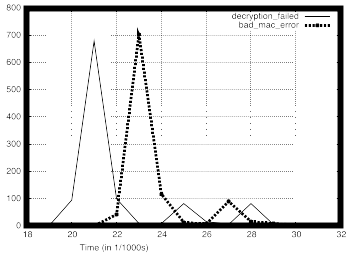
\includegraphics{aeinpractice/timing_tls}}
  \caption{Clear timing differences across error types in TLS provide a side-channel}
\label{fig:timing}
\end{figure}

The particular attack highighted in~\cite{Canvel2003} was fixed by RFC 5246, which required all padding errors to emit a MAC error to bring them in 
line with the secure theoretical model.  Despite this, channels for leaking information outside the scope of the model persist, including timing 
errors highlighted by the same work.  A clear separation in the timing of various error sources in TLS 1.2 was described by~\cite{Canvel2003}, and is 
shown in Figure~\ref{fig:timing}.  So, even returning the same error message may not suffice, and indeed RFC 5246 attempted to address this issue by 
requiring that ``implementations MUST ensure that record processing time is essentially the same whether or not the padding is correct."  The RFC 
noted that the MAC's performance differences under different data sizes still left a timing channel in place, but this was not believed to be 
exploitable.  In 2013, this was shown to be false, and another timing attack was shown in RFC 5246-compliant implementations~\cite{Fardan2013}.

TLS is not unique; SSH protocols underwent a similar series of attacks and ad-hoc countermeasures.  Bellare et al showed an attack as a case study of 
their original work on secure authenticated encryption in~\cite{Bellare2004}.  Specifically, the SSH binary packet protocol leaks the initialization 
vector of the next message to be encrypted to an adversary.  If the adversary can also control the full first block of input, the adversary 
essentially chooses the full input to the underlying deterministic block cipher, which can leak input about whether a queried message block was 
encrypted before, leaking plaintext information. The same work proposed a series of modifications to the protocol fixing the attack, claiming the new 
notion satisfied the most rigorous definition of provable security.

Similarly to the TLS case, an attack was later found in the ``fixed" scheme by Albrecht et al. in~\cite{Albrecht2009}, whereby a lack of ciphertext 
integrity in the scheme allowed an adversary to control the length field of the protocol's encoding, which had to be decoded before the message used 
to calculate the MAC was computed.  The value of this length field would then affect timings of SSH packets, which could be measured to infer its 
value.  This attack was missed by the original analysis of Bellare et al. that claimed the SSH protocol was secure, as there was no model for timing 
side channels in their adversary, and all decryption failure errors were treated as indistinguishable failures (sound familiar?).  These gaps were 
finally bridged by a formal analysis in~\cite{Paterson2010}.

By feeding random blocks of ciphertext in as the first block of a new session, and letting the protocol interpret them as a potential length field 
before throwing a MAC error, leakage about the plaintext data that originally formed these ciphertext blocks could be recovered.  Like the TLS case, 
this shows the danger of data encodings interacting with cryptographic primitives that do not provide appropriate authentication guarantees; as a 
practitioner implementing protocols based on cryptography, it is critical to rigorously evaluate the concrete security provided by any primitives used 
in the context of other interacting components, parsers, etc.

\subsection{Authenticated Encryption Extensions}

Because of the obvious popularity of authenticated encryption in securing communications, and its importance to deployed protocols, a number of 
variants of authenticated encryption and their associated security models have been studied in the literature.  We briefly mention a few, as well as 
provide intuition for key trade-offs in their design.

\textbf{Stateful encryption} All the constructions and games described in this chapter have assumed a random initialization vector used to provide 
security to e.g. repeated plaintext blocks.  The stateful variants of such schemes instead assume a recipient maintains some state, and do not 
transmit the initialization vector as the first block of ciphertext, instead using this state.  Security models for such schemes are complicated, as 
they need to handle e.g. reordering of messages from the sender to the receiver, ensuring no data is leaked.

\textbf{Nonce-Based AE(AD)} One natural question is whether AD schemes can be made deterministic, removing the need for randomness.  Currently, our 
e.g. ROR definitions require a random initialization vector to hide correlations in repeated message values.  An alternative construction first 
explored by Rogaway et. al in 2004~\cite{Rogaway2004} is the use of \emph{nonces}, or values used only once, in the place of initialization vectors. 
In these schemes, extended security definitions make the additional assumption that no nonce is used twice across encryptions.  In the event that a 
nonce is used twice, no security is provided whatsoever, regardless of whether the same or different messages are encrypted.  Additionally, such 
constructions have the benefit that good randomness is not required during encryption, removing many PRNG-based attacks which have led to IV reuse in 
practice.

\textbf{Misuse-resistant nonce-based AE(AD)} A natural extension of nonce-based AE is to extend the security definitions to cases where the nonce 
\emph{is} reused, minimizing the potential for damage in the event of misuse (or equivalently, in the case of IV reuse in a randomized setting).  Any 
nonce that is reused with the same message in a deterministic scheme will obviously leak plaintext equality, so leaking only this is both a natural 
and optimal security definition for such schemes.  To achieve this, we modify the security definitions shown to allow the adversary to make any number 
of encryption and decryption queries that may repeat IVs, and require encryption oracle responses to appear random except in the case of a repetition 
in all of $(header, IV, message)$.  Such schemes were first explored in depth in~\cite{Rogaway2006}.


\textbf{Trade-offs in Misuse-resistant nonce-based AE(AD)} Interestingly, the AE constructions we have explored showcase fundamental security 
trade-offs, as briefly explored in~\cite{Rogaway2006}.  In an encryption scheme used e.g. in an online communication protocol, it may be desireable 
for an encryption algorithm to return partial ciphertext results as plaintext blocks are encrypted, without waiting for the full message.  Such 
constructions are especially useful for resource constrained contexts, where maintaining state may be costly.  In such constructions, the ciphertext 
of the first block $C_1$ cannot be affected by subsequent message $M_n, n>1$ or ciphertext blocks $C_n, n>1$, as the algorithm outputs $C_1$ before 
receiving any such information; we refer to such schemes as \emph{online} schemes, or \emph{feed forward} schemes.  Obviously, this characteristic of 
an online deterministic encryption scheme means that plaintext prefix equality can be leaked when nonces are misused.  The intuition for this is 
clear; consider two messages that differ only in the last block, and note that if a nonce is reused in any deterministic feed forward construction 
over these messages, the first output block cannot depend on the last by nature of feed forward.  Indeed, online output will inherently be identical 
up to the first difference in the message input, leaking exactly equality of prefixes.

Offline constructions feed ciphertexts output by the first pass backwards, to ensure that each block of the message depends on every other block; in 
the above example, the last message block now affects every block of ciphertext.  While such constructions are inherently less efficient, as the first 
pass must complete before the second pass which depends on its full output, they are also inherently more secure, achieving the maximum possible 
security for deterministic encryption.  Nothing is leaked except in the case of re-used $(header, IV, message)$, which causes plaintext equality to 
leak.  Such leaks are unavoidable in any deterministic construction where all input is re-used.

\subsection{Choices for Practitioners}

\begin{table}[h]
\scalebox{.8}{
\begin{tabular}{llllll}
\textbf{Mode}     & \textbf{Inventors} & \textbf{Notes}                                                   & \textbf{Nonce-based} & \textbf{Misuse-resistant} & \textbf{Robust} \\
OCB               & Rogaway            & One-pass                                                         & \color{green}Yes\color{black}                  & No                        & No              \\
\specialcell{AES-CTR\\-then-HMAC} &                    &                                                                  & No                   & No                        & \color{green}Yes\color{black}*            \\
GCM               & McGrew, Viega      & \specialcell{CTR mode with Universal\\Hash Function-based MAC}        & \color{green}Yes\color{black}                  & No                        & No              \\
SIV               & Rogaway, Shrimpton & Not online, two full passes                                      & \color{green}Yes\color{black}                  & \color{green}Yes\color{black}                       & No              \\
AES-GCM-SIV       & Gueron, Lindell    & \specialcell{SIV using AES-GCM\\with special tweaks} & \color{green}Yes\color{black}                  & \color{green}Yes\color{black}                       & No              \\
ASCON             & Dobraunig et al.   & Based on lightweight cipher                                      & \color{green}Yes\color{black}                  & \color{orange}Except prefix\color{black}             & \color{green}Yes\color{black}             \\
AEGIS             & Wu, Preneel        & Uses AES round function                                          & \color{green}Yes\color{black}?                 & No                        & ???             \\
COLM              & Andreeva et al.    & Parallelizable cipher      & \color{green}Yes\color{black}                  & \color{orange}Except prefix\color{black}             & No?            
\end{tabular}
}
  \caption{Clear timing differences across error types in TLS provide a side-channel}
\label{table:practicalae}
\end{table}


Table~\ref{table:practicalae} summarizes several modes that have been cryptographically analyzed for security, as well as their inventors and notes on 
algorithm characteristics.

\subsection{Questions [Proofreaders; any suggestions?]}

\begin{itemize}
\item Consider the American Standards Committee ANSX9.102 document available at \url{https://eprint.iacr.org/2004/340.pdf}, which formalizes keywrap protocols using Misuse-resistant nonce-based AE(AD) as described above.  Categorize AKW1 and AKW2 as online or offline algorithms, and state precisely what is leaked by each in the event of both correct operation and misuse.
\item Consider the key reuse adversary described by Figure~\ref{fig:reuseadversary}, and the scheme described by Figure~\ref{fig:reusescheme}.  Extend the provided attack to a version of the scheme which only allows for messages with two message blocks (of length $2n$) by providing and justifying an adversary that wins the CTXT game.
\end{itemize}

\newpage
%%%%%%%%%%%%%%%%%%%%%%%%%%%%%%%%%%%%%%%%%%%%%%%%%%%%%%%%%%%%%%%%%%%%%%%%%%%%%%%%
\section{Cryptographic Hash Functions}
\label{sec:hashfunctions}

A cryptographic hash function is a map $H\Colon\msgspace\rightarrow\bits^n$ for
some set $\msgspace$ and number $n > 0$. Typical values of $n$ are these days
256, 512, etc., and most hash functions support an essentially unlimited messgae
space $\msgspace$, such as all strings of length up to $2^{64}-1$.

\fpage{.25}{
\underline{$\CR^\advA_{H}$}\\[1pt]
$(M,M') \getsr \advA$\\
If $M = M'$ then Ret $\false$\\
Ret $H(M) = H(M')$
}


\bnm
\AdvCR{H}{\advA} = \Prob{\CR^\advA_H\Rightarrow\true}
\enm




\fpage{.25}{
\underline{$\CR^\advA_{H,\ic}$}\\[1pt]
$E \getsr \blockciphers(k,n)$\\
$(M,M') \getsr \advA^{\ic,\icInv}$\\
If $M = M'$ then Ret $\false$\\
Ret $H^\ic(M) = H^\ic(M')$\medskip

\underline{$\ic(K,X)$}\\
Ret $\cipherE(K,X)$\medskip

\underline{$\icInv(K,Y)$}\\
Ret $\cipherD(K,Y)$
}

\begin{theorem*}
Let $f$ be the Davies-Meyer compression function built from a block cipher
$\cipherE\Colon\bits^k\times\bits^n\rightarrow\bits^n$ modeled as an ideal
cipher. For any adversary $\advA$ making at most~$q$ queries it holds that
\bnm
  \AdvCR{f}{\advA} \le \frac{(q+1)(q+2)}{2^n} \;.
\enm
\end{theorem*}

\begin{proof}
Assume $\advA$ that outputs $(Y,M)$ and $(Y',M')$ has already queried $\cipherE$
or $\cipherD$ for associated points. This can be argued easily by reducing to
by making at most $q' = q+2$ queries. We also assume
$\advA$  Then each query defines a triple 
$(K_i,X_i,Y_i)$ where either $Y_i = \cipherE(K_i,X_i)$ was queried or $X_i =
\cipherD(K_i,Y_i)$ was queried. For a collision to occur it must be that there
exist indices $i,j$ such that $X_i \oplus Y_i = X_j \oplus Y_j$, to arrange that
$X_i \oplus \cipherE(K_i,X_i) = X_j \oplus \cipherE(K_j,X_j)$. Let $C_j$ be the
event that such a collision occurs upon a query the $j\thh$ query. Then we have
that $X_i,Y_i$ are at this point fixed values while exactly one of $X_j$ or
$Y_j$ is a fixed value, with the other being a uniformly chosen point subject
only to permutivity. Then we have that 
\begin{align*}
\Prob{\CR_{f,\cipherE}^\advA\Rightarrow\true} 
  &\le \sum_{j=1}^{q'} \Prob{C_j}   \\
  &\le \sum_{j=1}^{q'} \frac{j-1}{2^n-j+1}\\
  &\le \sum_{j=1}^{q'} \frac{j-1}{2^n-q'}\\
  &= \frac{q'(q'-1)}{2(2^n-q')}
  &= \frac{(q+2)(q+1)}{2^n} 
\end{align*}
\end{proof}


\begin{theorem*}
Let $f$ be a compression function and $H$ be the MD hash function built from it. 
Let $\advA$ be a $\CR_H$-adversary outputing messages eacah of length at most $\sigma$
blocks after MD padding. Then we give an $\CR_f$-adversary $\advB$
such that
\bnm
  \AdvCR{\advA}{H} \le \AdvCR{\advB}{f} \;.
\enm
Adversary~$\advB$ runs in time that of $\advA$ plus at most $2\sigma$ computations of
$f$.
\end{theorem*}


\fpage{.25}{
\underline{$\CR^\advA_{H,\ic}$}\\[1pt]
$E \getsr \blockciphers(k,n)$\\
$(M,M') \getsr \advA^{\ic,\icInv}$\\
If $M = M'$ then Ret $\false$\\
Ret $H^\ic(M) = H^\ic(M')$\medskip

\underline{$\ic(K,X)$}\\
If $\TabE[K,X] \ne \bot$ then\\
\myInd $Y \getsr \Range[K]$\\
\myInd $\TabE[K,X] \getsr Y$\\
\myInd $\TabD[K,Y] \getsr X$\\
\myInd $\Domain[K] \getu X$\\
\myInd $\Range[K] \getu Y$\\
Ret $\TabE[K,X]$\medskip

\underline{$\icInv(K,Y)$}\\
If $\TabD[K,Y] \ne \bot$ then\\
\myInd $X \getsr \Domain[K]$\\
\myInd $\TabE[K,X] \gets Y$\\
\myInd $\TabD[K,Y] \gets X$\\
\myInd $\Domain[K] \getu X$\\
\myInd $\Range[K] \getu Y$\\
Ret $\TabD[K,Y]$
}

\newpage
%%%%%%%%%%%%%%%%%%%%%%%%%%%%%%%%%%%%%%%%%%%%%%%%%%%%%%%%%%%%%%%%%%%%%%%%%%%%%%%%
\section{Further Security Properties for Hash Functions}
\label{sec:hashfunctions}

\fpage{.25}{
\underline{$\OWF^\advA_{H}$}\\[1pt]
$M \getsr \msgspace$\\
$Y \gets H(M)$\\
$M' \getsr \advA(Y)$\\
Ret $(H(M') = Y)$
}


\bnm
\AdvOWF{H}{\advA} = \Prob{\OWF^\advA_H\Rightarrow\true}
\enm



\fpage{.25}{
\underline{$\SPR^\advA_{H}$}\\[1pt]
$M \getsr \msgspace$\\
$Y \gets H(M)$\\
$M' \getsr \advA(M)$\\
Ret $(H(M') = H(M)) \land (M \ne M')$
}


\bnm
\AdvSPR{H}{\advA} = \Prob{\SPR^\advA_H\Rightarrow\true}
\enm


\fpage{.25}{
\underline{$\PWR^\advA_{H,p}$}\\[2pt]
$\pw \get{p} \msgspace$\\
$\salt \getsr \bits^n$\\
$Y \gets H(\salt \concat M)$\\
$\pw' \getsr \advA(\salt,Y)$\\
Ret $(\pw' = \pw)$
}

\fpage{.25}{
\underline{$\PWR^\advA_{\Horacle,p}$}\\[2pt]
$\pw \get{p} \msgspace$\\
$\salt \getsr \bits^n$\\
$Y \gets \Horacle(\salt \concat M)$\\
$\pw' \getsr \advA^\Horacle(\salt,Y)$\\
Ret $(\pw' = \pw)$\medskip

\underline{$\Horacle(M)$}\\
If $\TabH[M] = \bot$ then\\
\myInd $\TabH[M] \getsr \bits^n$\\
Ret $\TabH[M]$
}

\begin{theorem*}
Let $H\Colon\msgspace\rightarrow\bits^n$ and $\advA$ be a $\SPR_H$-adversary.
Then we give a $\CR_H$-adversary $\advB$ such that
\bnm 
  \AdvSPR{H}{\advA} \le \AdvCR{H}{\advB}
\enm
Adversary~$\advB$ runs in time that of $\advA$. 
\end{theorem*}


\paragraph{Application: password recovery.}
The min-entropy of a distribution $p$ is the probability that one can guess a
value chosen according to $p$ in a single guess. Mathematically:

\bnm
  \Hinfty(p) = -\max_{x} \log \frac{1}{p(x)}
\enm
Not to be confused with Shannon entropy:

\bnm
  \Hshan(p) =  \sum_x p(x) \log \frac{1}{p(x)}
\enm

\begin{theorem}
Let $\Horacle\Colon\msgspace\rightarrow\bits^n$ be modeled as a random oracle
and $p$ be a distribution over $\msgspace$.
Then for any $\PWR_{\Horacle,p}$-adversary $\advA$ making at most $q$ queries 
it holds that
\bnm
  \AdvPWR{\Horacle,p}{\advA} \le \frac{q}{2^{\mu(p)}} \;.
\enm
\end{theorem}



\hfpages{.25}{
\underline{$\PRF1_{F,\Horacle}^\advA$}\\
$K \getsr \keyspace$\\
$b' \getsr \advA^{\Fn,\Horacle}$\\
Return $b'$\medskip

\underline{$\Fn(M)$}\\
Return $F^\Horacle_K(M)$\medskip

\underline{$\Horacle(X)$}\\
If $\TabH[X] = \bot$ then\\
\myInd $\TabH[X] \getsr \bits^n$\\
Ret $\TabH[X]$

}{
\underline{$\PRF0_{F,\Horacle}^\advA$}\\
$\rho \getsr \Func(\msgspace,n)$\\
$b' \getsr \advA^{\Fn,\Horacle}$\\
Return $b'$\medskip

\underline{$\Fn(M)$}\\
Return $\rho(M)$\\

\underline{$\Horacle(X)$}\\
If $\TabH[X] = \bot$ then\\
\myInd $\TabH[X] \getsr \bits^n$\\
Ret $\TabH[X]$
}


\begin{theorem}
Let  $\Horacle\Colon\msgspace\rightarrow\bits^n$ be modeled as a random oracle
and let $F^\Horacle\Colon\keyspace\times\msgspace\rightarrow\bits^n$ be the
hash-based PRF defined as $F^\Horacle(K,M) = \Horacle(K \concat M)$. 
Then for any $\PRF_{F,\Horacle}$-adversary $\advA$ making at most $q$ queries 
to $\Horacle$ it holds that
\bnm
  \AdvPRF{F,\Horacle}{\advA} \le \frac{q}{|\keyspace|} \;.
\enm
\end{theorem}



\hfpages{.25}{
\underline{$\INDIFF1_{H,\foracle}^\advD$}\\
$b' \getsr \advD^{\Fn,\foracle}$\\
Ret $b'$\medskip

\underline{$\Fn(M)$}\\
Ret $H^\foracle(M)$\medskip

\underline{$\foracle(X)$}\\
If $\Tabf[X] = \bot$ then\\
\myInd $\Tabf[X] \getsr \bits^n$\\
Ret $\Tabf[X]$
}{
\underline{$\INDIFF0_{\Horacle,\simu}^\advD$}\\
$b' \getsr \advD^{\Fn,\simoracle}$\\
Return $b'$\medskip

\underline{$\Fn(M)$}\\
If $\TabH[M] = \bot$ then\\
\myInd $\TabH[M] \getsr \bits^n$\\
Ret $\TabH[M]$\medskip

\underline{$\simoracle(X)$}\\
Ret $\simu^\Fn(X)$
}


\bnm
  \AdvINDIFF{H,\foracle,\simu}{\advA} =
    \left|\Prob{\INDIFF1_{H,\foracle}^\advD\Rightarrow1} -
            \Prob{\INDIFF0_{\Horacle,\simu}^\advD\Rightarrow1}\right|
\enm


\hfpages{.20}{
\underline{$\RKAPRF1_{F,\Phi}^\advA$}\\
$K \getsr \keyspace$\\
$b' \getsr \advA^{\Fn}$\\
Ret $b'$\medskip

\underline{$\Fn(\phi,X)$}\\
If $\phi \notin \Phi$ then\\
\myInd Ret $\bot$\\
Ret $F(\phi(K),X)$
}{
\underline{$\RKAPRF0_{F,\Phi}^\advA$}\\
$K \getsr \keyspace$\\
$\rho \getsr \Func(\keyspace\times\msgspace,n)$\\
$b' \getsr \advA^{\Fn}$\\
Ret $b'$\medskip

\underline{$\Fn(\phi,X)$}\\
If $\phi \notin \Phi$ then\\
\myInd Ret $\bot$\\
Ret $\rho(\phi(K),X)$
}



%!TEX root = ../main.tex
%%%%%%%%%%%%%%%%%%%%%%%%%%%%%%%%%%%%%%%%%%%%%%%%%%%%%%%%%%%%%%%%%%%%%%%%%%%%%%%%
\tikzset{XOR/.style={thick,
					draw,
					circle,
					append after command={
					        [shorten >=\pgflinewidth, shorten <=\pgflinewidth,]
					        (\tikzlastnode.north) edge[thick] (\tikzlastnode.south)
					        (\tikzlastnode.east) edge[thick] (\tikzlastnode.west)
        				},
    				},
}

%!TEX root = ../main.tex
%%%%%%%%%%%%%%%%%%%%%%%%%%%%%%%%%%%%%%%%%%%%%%%%%%%%%%%%%%%%%%%%%%%%%%%%%%%%%%%%
\subsection{Building PRPs from PRFs}
In the previous section, we showed that it is hard to distinguish between a PRF and a PRP (see \lemref{switching-lem}).
However, as in the use case of block ciphers for length-preserving encryption and decryption, we specifically require a block cipher to be secure as a PRP for correctness purposes.
Specifically, we need to be able to correctly decrypt in most applications of block ciphers.
A natural question to ask is does the existence of a PRF imply the existence of a PRP, or more constructively, can we build a PRP given a PRF?

In this section, we will show that it is possible to build a PRP from a PRF.
We will examine one such construction called a Feistel network which is used in the construction of many early block ciphers, including DES (Data Encryption Standard), the first standardized block cipher.

\paragraph{Feistel networks.}
A Feistel round transforms an arbitrary function into a permutation.
Define $\cipher:\bits^k\times\braces*{0,1}^{2n}\rightarrow\braces*{0,1}^{2n}$ as the permutation constructed using one Feistel round with function $\prf:\braces*{0,1}^k\times\braces*{0,1}^n\rightarrow\braces*{0,1}^n$.
The function $\prf$ is known as the round function of the Feistel network.
\begin{wrapfigure}{r}{2in}
\center
\begin{tikzpicture}
    \node(r0) at ($(0,0)$)  {$R_0$};
    \node (l0) [left of = r0, node distance=3.0cm] {$L_0$};
    \node[draw,thick,minimum width=0.75cm] (\prf) [below of = r0, node distance=1.1cm]  {$\prf_{\prfkey}$};
    \node (xor) [XOR, below of = \prf, node distance = 0.75cm, scale=1.0] {};
    \node (junction0) [below of = r0, node distance = 0.5cm] {};
    \node (junction1) [below of = l0, node distance = 0.75cm] {};
    \node (junction2) [below of = l0, node distance = 1.5cm] {};
    \node (junction3) [left of = xor, node distance = 0.5cm] {};
    \path[->]
      (r0) edge[thick] node {} (\prf)
      (\prf) edge[thick] node {} (xor)
      (junction3.center) edge[thick] node {} (xor);
    \path[-]
      (l0.south) edge[thick] node {} (junction1.center)
      (junction0.center) edge[thick] node {} (junction2.center)
      (junction1.center) edge[thick] node {} (junction3.center);
    \node (r1) [below of = xor, node distance=0.75cm] {$R_1$};
    \node (l1) [left of = r1, node distance=3.0cm] {$L_1$};
    \path[->]
      (xor) edge[thick] node {} (r1)
      (junction2.center) edge[thick] node {} (l1);
\end{tikzpicture}
\caption{A single round of a Feistel network.}
\label{fig:feistel-1}
\end{wrapfigure}
This construction is depicted in Figure~\ref{fig:feistel-1} where $2n$ bit inputs and outputs are split into left and right parts of length $n$ notated $L_0, R_0$ and $L_1, R_1$, respectively.
Function $\prf$ is notated with fixed key $\prfkey$ as $\prf_{\prfkey}:\braces*{0,1}^n\rightarrow\braces*{0,1}^n$.
The Feistel round is then
\begin{align*}
L_1 &\gets R_0\\
R_1 &\gets L_0 \oplus \prf_{\prfkey}(R_0)\,.
\end{align*}


\begin{example}[1-round Feistel network is a permutation]
  First, let us see why the Feistel construction builds a permutation from an arbitrary function.
  Notice that as long as the round function $\prf_{\prfkey}$ is defined on all inputs from domain $\braces*{0,1}^n$ then $\cipher$ is defined on all inputs from domain $\braces*{0,1}^{2n}$.
  Next, we show that any output of $\cipher$, $L_1\concat R_1$, corresponds to a unique input $L_0\concat R_0$.
  Even though $\prf_{\prfkey}$ is not assumed to be invertible, since the input to $\prf_{\prfkey}$, $R_0$, is passed directly to the output as $L_1$, we can invert by computing
  \bnm
    L_0 \gets R_1\oplus \prf_{\prfkey}(L_1)\hspace{2em}\text{and}\hspace{2em} R_0 \gets L_1\,.
  \enm
  These two properties together mean $\cipher$ is a complete permutation on $\braces*{0,1}^{2n}$.
\end{example}

  However, a 1-round Feistel network $\cipher$ is not a PRP.
  To show this, consider the following PRP adversary $\advA$ for domain $\braces*{0,1}^{2n}$:
  \begin{center}
    \fpage{.2}{
    \underline{\textbf{adversary }$\advA^{\Fn}$}\\[2pt]
    $(L_1,R_1)\gets\Fn(0^{2n})$\\
    Return $L_1 = 0^{n}$
    }
  \end{center}

  \noindent In $\PRP1$, where the oracle $\Fn$ returns $\cipher_{\prfkey}(0^{2n})$, $\advA$ returns 1 with probability 1.
  In $\PRP0$, where oracle $\Fn$ returns a random value, the probability $\advA$ returns 1 is the probability that the first $n$ bits of the random output are 0.
  Thus,
\begin{align*}
\AdvPRP{\cipher}{\advA} &= \absv*{\Prob{\PRP1_\cipher^\advA\Rightarrow 1} - \Prob{\PRP0_\cipher^\advA\Rightarrow1} }\\
&= 1 - \frac{1}{2^n}\,.
\end{align*}
We see that it is trivial to distinguish a 1-round Feistel network from a random permutation, since the second half of the input is mapped directly to the first half of the output.
Does the randomness of the permutation improve by performing numerous Feistel rounds?
One way to construct a multi-round Feistel network is by feeding the outputs of the previous round as inputs to the next round, where each round is keyed with an independent key.
To use only a single key, we could consider an alternate construction, where the round function $\prf$ in each Feistel round has a different domain, $\prf:\braces{0,1}^{k}\times\braces{0,1}^{2n}\rightarrow\braces{0,1}^n$.
As before, the round function will take in the second half of the input, but it will also take in an $n$-bit round counter.
To stack Feistel rounds into a multi-round Feistel network, we simply ensure that each round uses a different round counter.
Figure~\ref{fig:feistel-3} depicts a 3-round Feistel network constructed in this manner.
It turns out that three rounds are necessary to create a PRP using a Feistel network.
We leave showing a PRP distinguishing adversary for the 2-round Feistel network as an exercise to the reader.

%!TEX root = ../main.tex
%%%%%%%%%%%%%%%%%%%%%%%%%%%%%%%%%%%%%%%%%%%%%%%%%%%%%%%%%%%%%%%%%%%%%%%%%%%%%%%%
\paragraph{3-round Feistel network is a PRP}
Next, we show that given PRF security of the underlying round function, a 3-round Feistel network is a PRP.
Intuitively, the proof will follow the intuition that 3 rounds of Feistel allows the round function to properly add randomness to both $L_3 = R_2$ and $R_3$.
In particular, we want to show that the output of the $\prf_{\prfkey}(\langle 2 \rangle\concat R_1)$ and $\prf_{\prfkey}(\langle 3 \rangle\concat R_2)$ cannot be effectively controlled by adversary $\advA$, i.e., $\advA$ cannot create collisions on $R_1$ and $R_2$.

\begin{theorem}[Luby-Rackoff]\label{thm:luby-rackoff}
Let $\Feistel$ be the 3-round Feistel cipher using round function
$\prf\Colon\bits^k\times\bits^{2n}\rightarrow \bits^n$. For any
$\PRP_\cipher$-adversary $\advA$ making at most $q$ queries
we give a $\PRF_{\prf}$-adversary $\advB$ making at most $3q$ queries such that
\bnm
  \AdvPRP{\Feistel}{\advA} \le \AdvPRF{\prf}{\advB} + \frac{2q^2}{2^n} +
  \frac{q^2}{2^{2n}} \;.
\enm
\end{theorem}
\scribenote{How are we doing cites? (Luby-Rackoff)}

\begin{proof}
Without loss of generality, we consider an adversary $\advA$ that only makes unique queries to oracle $\Fn$.
\scribenote{Be more formal about why this okay?} \pfreadernote{Looking at the Boneh-Shoup explanation for this, I think it would be better to be more clear on why this is ok}
We bound the advantage of $\PRP$ adversary $\advA$ by bounding its advantage in each game in a series of game hops.
Pseudocode for these games is given in Figure~\ref{fig:games-luby-rackoff}.

Game $\G0$ is constructed exactly as $\PRP1^{\advA}_{\Feistel}$; the oracle pseudocode expands out the computation of the 3-round Feistel network $\Feistel$:
\bnm
\Prob{\PRP1_\Feistel^\advA\Rightarrow 1} = \Prob{\G0\Rightarrow 1}.
\enm
Game $\G1$ replaces the round function $\prf$ with a random function $\randfn$ mapping from $\braces{0,1}^{2n}\rightarrow\braces{0,1}^n$.
\scribenote{Should PRF security game be defined with respect to different domain and range space, $m$ and $n$?}
We bound the ability to distinguish between $\G0$ and $\G1$ by the PRF security of $\prf$.
Consider the following PRF adversary $\advB$ which runs $\advA$ with a simulated oracle $\FnSim$.

\begin{center}
\fpage{.22}{
\underline{$\advB^\Fn$}\\[2pt]
$K \getsr \bits^k$\\
$b' \getsr \advA^\FnSim$\\
Return $b'$\medskip

\underline{$\FnSim(\msg)$}\\
$L_1 \gets R_0$\\
$R_1 \gets L_0 \oplus \Fn(\langle 1\rangle \concat R_0)$\\
$L_2 \gets R_1$\\
$R_2 \gets L_1 \oplus \Fn(\langle 2\rangle \concat R_1)$\\
$L_3 \gets R_2$\\
$R_3 \gets L_2 \oplus \Fn(\langle 3\rangle \concat R_2)$\\
Return $L_3 \concat R_3$
}
\end{center}
\pfreadernote{Should this game be a figure?} \pfreadernote{Julia: since it's just an adversary, it's probably ok?}
Adversary $\advB$ simulates $\FnSim$ by running the 3-round Feistel network but replacing the round function with a call to its own oracle $\Fn$.
In \PRF0, where $\advB$'s oracle $\Fn$ acts as the round function $\prf$, $\advB$ runs exactly $\G0$.
In \PRF1, where $\Fn$ acts as a random function $\rho$, $\advB$ runs exactly $\G1$.
Thus, we have
\begin{align*}
\AdvPRF{\prf}{\advB} &= \absv*{\Prob{\PRF1_\prf^\advB\Rightarrow 1} - \Prob{\PRF0_\prf^\advB\Rightarrow1}}\\
&= \absv*{\Prob{\G1\Rightarrow 1} - \Prob{\G0\Rightarrow1}}.\\
\end{align*}

\begin{figure}[t]
\hfpagessss{.20}{.20}{.20}{.25}{
\underline{$\G0$}\\[2pt]
$K \getsr \bits^k$\\
$b' \getsr \advA^\Fn$\\
Return $b'$\medskip

\underline{$\Fn(\msg)$}\\
$(L_0, R_0) \gets \msg$\\
$L_1 \gets R_0$\\
$R_1 \gets L_0 \oplus F_K(\langle 1\rangle \concat R_0)$\\
$L_2 \gets R_1$\\
$R_2 \gets L_1 \oplus F_K(\langle 2 \rangle \concat R_1)$\\
$L_3 \gets R_2$\\
$R_3 \gets L_2 \oplus F_K(\langle 3 \rangle \concat R_2)$\\
Return $L_3 \concat R_3$
}{
\underline{$\G1$}\\[2pt]
$\rho \getsr \Func(2n,n)$\\
$b' \getsr \advA^\Fn$\\
Return $b'$\medskip

\underline{$\Fn(\msg)$}\\
$(L_0, R_0) \gets \msg$\\
$L_1 \gets R_0$\\
$R_1 \gets L_0 \oplus \rho(\langle 1\rangle \concat R_0)$\\
$L_2 \gets R_1$\\
$R_2 \gets L_1 \oplus \rho(\langle 2 \rangle \concat R_1)$\\
$L_3 \gets R_2$\\
$R_3 \gets L_2 \oplus \rho(\langle 3 \rangle \concat R_2)$\\
Return $L_3 \concat R_3$
}{
\underline{$\fbox{\G2}$\;\;\;\G3}\\[2pt]
$b' \getsr \advA^\Fn$\\
Return $b'$\medskip

\underline{$\Fn(\msg)$}\\
$(L_0, R_0) \gets \msg$\\
$L_1 \gets R_0$\\
If $\TabF[\langle1\rangle\concat R_0] = \bot$ then\\
\ind $\TabF[\langle1\rangle\concat R_0] \getsr \bits^n$\\
$X_1 \gets \TabF[\langle1\rangle\concat R_0]$\\
$R_1 \gets L_0 \oplus X_1$\\
$L_2 \gets R_1$\\
$X_2 \getsr \bits^n$\\
If $\TabF[\langle2\rangle\concat R_1] \ne \bot$ then\\
\ind $\badtrue$\\
\ind \fbox{$X_2 \gets \TabF[\langle2\rangle\concat R_1]$}\\
$\TabF[\langle2\rangle\concat R_1] \gets X_2$\\
$R_2 \gets L_1 \oplus X_2$\\
$L_3 \gets R_2$\\
$X_3 \getsr \bits^n$\\
If $\TabF[\langle3\rangle\concat R_2] \ne \bot$ then\\
\ind $\badtrue$\\
\ind \fbox{$X_3 \gets \TabF[\langle3\rangle\concat R_2]$}\\
$\TabF[\langle3\rangle\concat R_2] \gets X_3$\\
$R_3 \gets L_2 \oplus X_3$\\
Return $L_3 \concat R_3$
}{
\underline{$\G3$\;\;\;$\fbox{\G4}$}\\[2pt]
$b' \getsr \advA^\Fn$\\
Return $b'$\medskip

\underline{$\Fn(\msg)$}\\
$(L_0, R_0) \gets \msg$\\
$L_1 \gets R_0$\\
If $\TabF[\langle1\rangle\concat R_0] = \bot$ then\\
\ind $\TabF[\langle1\rangle\concat R_0] \getsr \bits^n$\\
$X_1 \gets \TabF[\langle1\rangle\concat R_0]$\\
$R_1 \gets L_0 \oplus X_1$\\
$L_2 \gets R_1$\\
$X_2 \getsr \bits^n$\\
If $\TabF[\langle2\rangle\concat R_1] \ne \bot$ then\\
\ind $\badtrue$\\
$\TabF[\langle2\rangle\concat R_1] \gets X_2$\\
$R_2 \gets L_1 \oplus X_2$;\;\;\fbox{$R_2 \getsr \bits^n$}\\
$L_3 \gets R_2$\\
$X_3 \getsr \bits^n$\\
If $\TabF[\langle3\rangle\concat R_2] \ne \bot$ then\\
\ind $\badtrue$\\
$\TabF[\langle3\rangle\concat R_2] \gets X_3$\\
$R_3 \gets L_2 \oplus X_3;$\;\;\fbox{$R_3 \getsr \bits^n$}\\
Return $L_3 \concat R_3$
}
\caption{Games for proof of 3-round Feistel network as PRP (Theorem~\ref{thm:luby-rackoff})}
\label{fig:games-luby-rackoff}
\end{figure}

In games $\G2$ and $\G3$, we use a similar trick to the one we used in our proof of the PRF-PRP switching lemma.
Game $\G2$ replaces the random function $\rho$ with a lazy evaluation of a random function using a table $\TabF$.
When the random function is queried on an input, the value in $\TabF$ keyed by the input is returned.
If there is no such value, meaning the input has not been previously queried, a new random value is generated, returned, and stored in $\TabF$ for future queries.
Thus, lazily building out $\TabF$ is equivalent to using random function $\rho$:
\bnm
\Prob{\G1\Rightarrow 1} = \Prob{\G2\Rightarrow 1}.
\enm

Game $\G3$ generates fresh random values on every input to the second and third round functions.
This is in contrast to $\G2$ where a fresh random value is only returned for inputs that have never been seen.
Thus, the difference between $\G2$ and $\G3$ occur when repeat inputs are used with the second or third round functions, which corresponds to repeat values of $R_1$ and $R_2$, respectively.
Intuitively, since we are only considering adversaries $\advA$ that make unique queries to $\Fn$, finding repeat values of $R_1$ and $R_2$ is hard because they both include randomness from the random function.
The pseudocode in Figure~\ref{fig:games-luby-rackoff} captures the event of a repeat query by a setting a $\bad$ flag.
The only difference between $\G2$ and $\G3$ occur after the $\bad$ flag is set; $\G2$ returns the consistent value from the look-up table $\TabF$, while $\G3$ returns a fresh random value.
Then by the fundamental lemma of game-playing,
\bnm
\absv*{\Prob{\G3\Rightarrow 1} - \Prob{\G2\Rightarrow1}} \le \Prob{\G3 \setsbad}.
\enm

Game $\G4$ is the same as $\G3$ except $R_2$ and $R_3$ are set to fresh random values.
In $\G3$, we have $R_2\gets L_1\oplus X_2$ and $R_3\gets L_2\oplus X_3$ for fresh random values $X_2,X_3$.
Thus, the probability space of $R_2$ and $R_3$ are the same and $\G4$ is identical to $\G3$:
\bnm
\Prob{\G3\Rightarrow 1} = \Prob{\G4\Rightarrow 1}.
\enm
Importantly, this also implies
\bnm
\Prob{\G3 \setsbad} = \Prob{\G4 \setsbad}.
\enm

Notice that $\G4$ simply returns a fresh random string of length $2n$ on every query to oracle $\Fn$.
Since we assume $\advA$ only makes unique queries to $\Fn$, $\G4$ is simulating a perfect random function, and thus is equivalent to the \PRF0 game:
\bnm
\Prob{\G4\Rightarrow 1} = \Prob{\PRF0^{\advA}_{\Feistel}\Rightarrow 1}.
\enm

And by the PRF-PRP switching lemma,
	\bnm
	\absv*{\Prob{\PRF0_{\Feistel}^{\advA}\Rightarrow 1} - \Prob{\PRP0_{\Feistel}^{\advA}\Rightarrow1}} \le \frac{q^2}{2^{2n}}  \;.
	\enm

Lastly, we can bound the probability that $\G4\setsbad$.
First, consider the probability $\G4\setsbad$ on query $i$; call this event $W_i$.
This event can be considered as two separate events depending on where the $\bad$ flag is set:
denote the event that $R_1$ collides as $W_i^1$ and the event that $R_2$ collides as $W_i^2$.

It is simple to bound the probability of $W_i^2$.
The probability of $R_2 = L_1 \xor X_2$ colliding with a previous $R_2$ on query $i$ is bounded by $q/2^n$ since $X_2$ is a fresh random string. \pfreadernote{$\G4$ just samples $R_2$ randomly, not $R_2 = L_1 \xor X_2$ so it might be good to refresh the reader's memory that we're using Pr[G3 sets bad] = Pr[G4 sets bad] here. Also maybe mention union bound for how you upper bounded the probability?}

Bounding the probability of $W_i^1$ is more nuanced.
At first glance, it appears that the logic should follow symmetrically to that from above where $R_1 = L_0\xor X_1$ for random $X_1$.
To bound the probability of collision to $q/2^n$, we must argue that $X_1$ is independent of the inputs to $\Fn$.
In the previous case, $X_2$ is freshly sampled on every query to $\Fn$ so independence is trivially satisfied.
This is not the case for $X_1$.
However, we can argue that $\advA$'s queries are dependent only on $\advA$'s random coins and the previous outputs of $\Fn$.
Since in $\G4$ the outputs of $\Fn$ are independently drawn random samples, we have that the inputs of $\Fn$ are independent of $X_1$.
\scribenote{May need to argue this more formally?}

Thus, by two applications of the union bound, we have
\pfreadernote{specify that initial value for sum is i=1 below}
\begin{align*}
  \Prob{\G4 \setsbad} &\le \sum_i^q \Prob{W_i}\\
  &\le \sum_i^q \Prob{W_i^1} + \Prob{W_i^2}\\
  &\le \sum_i^q \frac{q}{2^n} + \frac{q}{2^n}\\
  &= \frac{2q^2}{2^n}.
\end{align*}

Finally, to put it all together,

\begin{align*}
\AdvPRP{\Feistel}{\advA}
    &=\left|\Prob{\PRP1^\advA_\Feistel} - \Prob{\PRP0^\advA_\Feistel}\right|\\
    &= \left|\Prob{\G0} - \Prob{\PRP0^\advA_\cipher}\right|\\
    &\le \left|\Prob{\G1} + \AdvPRF{F}{\advB} - \Prob{\PRP0^\advA_\cipher}\right|\\
    &=   \left|\Prob{\G2} + \AdvPRF{F}{\advB} - \Prob{\PRP0^\advA_\cipher}\right|\\
    &\le \left|\Prob{\G3} + \Prob{\G3\setsbad} + \AdvPRF{F}{\advB} - \Prob{\PRP0^\advA_\cipher}\right|\\
    &= \left|\Prob{\G4} + \Prob{\G4\setsbad} + \AdvPRF{F}{\advB} - \Prob{\PRP0^\advA_\cipher}\right|\\
    &\le \left|\Prob{\G4} + \frac{2q^2}{2^n} + \AdvPRF{F}{\advB} - \Prob{\PRP0^\advA_\cipher}\right|\\
    &\le \left|\Prob{\PRP0^\advA_\cipher} + \frac{q^2}{2^{2n}} + \frac{2q^2}{2^n} + \AdvPRF{F}{\advB} - \Prob{\PRP0^\advA_\cipher}\right|\\
    &= \frac{q^2}{2^{2n}} + \frac{2q^2}{2^n} + \AdvPRF{F}{\advB}\\
\end{align*}

\end{proof}

\scribenote{Additional Exercise Ideas}
\begin{itemize}
  \item 2-round Feistel is not a PRP
  \item Show security of 3-round Feistel with 3 different keys
  \item What happens when same key is used across Feistel rounds? (I don't know)
  \item Show 3-round Feistel is not Strong PRP (Strong PRP gets access to both forward and inverse oracle) \pfreadernote{this would require providing strong PRP game}
  \item Show 4-round Feistel is Strong PRP
\end{itemize}

%!TEX root = ../main.tex
%%%%%%%%%%%%%%%%%%%%%%%%%%%%%%%%%%%%%%%%%%%%%%%%%%%%%%%%%%%%%%%%%%%%%%%%%%%%%%%%
\paragraph{Connection to card shuffling algorithms.}
\scribenote{TODO}

%!TEX root = ../main.tex
%%%%%%%%%%%%%%%%%%%%%%%%%%%%%%%%%%%%%%%%%%%%%%%%%%%%%%%%%%%%%%%%%%%%%%%%%%%%%%%%

\section*{Exercises}

\begin{enumerate}[label=\textbf{Exercise \thesection.\arabic*}, wide=0pt]
  \item Show the 2-round Feistel construction (with round counters) is not a PRP by providing a PRP-adversary that gets a large advantage.
  \item Show the PRP security of an alternate 3-round Feistel construction $\Feistel:\bits^{3k}\times\bits^{2n}\rightarrow\bits^{2n}$ with round function $\prf:\bits^k \times\bits^n\rightarrow\bits^n$ where each round is keyed by an independent key.
  How does the advantage bound for an adversary against this scheme compare to the bound showed for the round counter scheme?
  \item Consider the following \emph{strong PRP} security games which give the adversary access to both a forward oracle and inverse oracle.
  The distinguishing advantage of an adversary is defined in the same way as regular PRF and PRP security as the ability to distinguish between interacting with the cipher and interacting with a random permutation,
  $\AdvSPRP{\cipher}{\advA} = \left| \Prob{\SPRP1_\cipher^\advA\Rightarrow 1} - \Prob{\SPRP0_\cipher^\advA\Rightarrow1} \right|$.


	\begin{center}
	\hfpages{.13}{
		\underline{$\SPRP1_{\cipher}^\advA$}\\
		$K \getsr \keyspace$\\
		$b' \getsr \advA^\Fn$\\
		Return $b'$\medskip

		\underline{$\Fn(\msg)$}\\
		Return $\cipherE_K(\msg)$\medskip

		\underline{$\FnInv(\ct)$}\\
		Return $\cipherE_K^{-1}(\ct)$
	}{
		\underline{$\SPRP0_{\cipher}^\advA$}\\
		$\pi \getsr \Perm(n)$\\
		$b' \getsr \advA^\Fn$\\
		Return $b'$\medskip

		\underline{$\Fn(\msg)$}\\
		Return $\pi(\msg)$\medskip

		\underline{$\FnInv(\ct)$}\\
		Return $\pi^{-1}(\ct)$
	}
\end{center}

  Show the 3-round Feistel construction (with round counters) is not a strong PRP by providing a \SPRP-adversary.
  \item Show the 4-round Feistel construction (with round counters) is a strong PRP.
\end{enumerate}


\newpage
\section{PRFs from Hash functions}

\subsection{Other Hash based PRFs}
The Merkle Damg{\aa}rd construction from the previous section is a type of Prefix MAC (since the key is prepended to the message). Although the construction is secure PRF in the random oracle model, we saw how it is susceptible to length extension attacks. Several alternatives have been proposed to counter these attacks. 

\paragraph{Suffix MAC:}
$\hash^f(M \Vert K)$ - The key is appended to the end instead of the beginning. Now, for a length extension attack to succeed, the adversary must find a collision for hash output until the key is added. To elaborate, if the adversary finds messages $M_0$ and $M_1$ such that $\hash^f(M_0) = \hash^f(M_1)$ by an offline collision attack, then it can break security for the overall construction without ever needing the key. To prove \PRF-security, therefore, we require that $\hash$ be collision resistant.


\paragraph{Envelope MAC:} $\hash^f(K_1 \Vert M \Vert K_2)$ - A key $K_1$ is prepended and another key $K_2$ is appended to the input. The \PRF-security proof is similar to the one before except now collision resistance is no longer required.

\paragraph{Nested MAC:}
$\hash^f(K_1 \Vert \hash^f(K_2 \Vert M))$ - The standard Prefix MAC construction is applied to the message twice with two \textit{independently} chosen keys $K_1$ and $K_2$.


\subsection{The HMAC Construction}

$\HMAC$, a widely used MAC in practice is a close variant of the nested MAC. For $\HMAC$, The keys $K_1$ and $K_2$ are no longer picked independently but rather derived from some base key $K$. The keys are computed as $K_1 = f(\IV, K \oplus \ipad)$ and $K_2 = f(\IV, K \oplus \opad)$ where $\ipad$ (inner pad) and $\opad$ (outer pad) are constants. Figure \ref{fig: HMAC construction} shows both a shortened and an extended version of the $\HMAC$ construction

\begin{figure}[h]
\centering
\subcaptionbox{%
    % 
    \label{fig:HMAC 1}
  }[0.3\linewidth] {
   \begin{tikzpicture}[scale=0.4]
            \begin{scope}[]
                \node [draw,trapezium,trapezium left angle=70,trapezium right angle=70,minimum height=0.75cm,thick,fill=orange!15,shift={(1.15,0)},rotate=-90] 
                {\begin{sideways}\Large $\hash$ \end{sideways}};
                \draw[->,thick] (0,0) node[left] {$K_1 \Vert M $} -- (1.9,0);
                \draw[->,thick] ++(4,0) -- ++(1.5,0) -- ++(0,-2.5);
            \end{scope}
            \begin{scope}[shift={(6.2,-3.25)}]
                \node [draw,trapezium,trapezium left angle=70,trapezium right angle=70,minimum height=0.75cm,thick,fill=orange!15,shift={(1.15,0)},rotate=-90] 
                {\begin{sideways}\Large $\hash$ \end{sideways}};
                \draw[->,thick] (0,0) node[left] {$K_2 \Vert h$} -- (1.9,0);
                \draw[->,thick] ++(4,0) -- ++(2,0) node[right] {$Y$};
            \end{scope}
        \end{tikzpicture}
    }
\hfill
\subcaptionbox{%
   % \label{fig:HMAC 2}
  }[0.5 \linewidth]
  { 
  \begin{tikzpicture}[scale=0.4]
            \begin{scope}[]
                \node [draw,trapezium,trapezium left angle=50,trapezium right angle=90,minimum height=0.5cm,thick,fill=orange!15,shift={(1.15,0.3)},rotate=-90] 
                {\begin{sideways}\Large$f$\end{sideways}};
                \draw[->,thick] ++(0.5,+3) node[above] {$K \oplus \ipad$} -- ++(0,-1) -- ++(1.7,0);
                \draw[->,thick] ++(0,0.5) node[left] {IV} -- ++(2.2,0);
            \end{scope}

            \begin{scope}[shift={(3.5,0)}]
                \node [draw,trapezium,trapezium left angle=50,trapezium right angle=90,minimum height=0.5cm,thick,fill=orange!15,shift={(1.15,0.3)},rotate=-90] 
                {\begin{sideways}\Large$f$\end{sideways}};
                \draw[->,thick] ++(0.5,+3) node[above] {$M_1$} -- ++(0,-1) -- ++(1.7,0);
                \draw[->,thick] ++(0,0.5) -- node[below] {$K_1$} ++(2.2,0);
            \end{scope}

            \begin{scope}[shift={(7,0)}]
                \node [draw,trapezium,trapezium left angle=50,trapezium right angle=90,minimum height=0.5cm,thick,fill=orange!15,shift={(1.15,0.3)},rotate=-90] 
                {\begin{sideways}\Large$f$\end{sideways}};
                \draw[->,thick] ++(0.5,+3) node[above] {$M_2$} -- ++(0,-1) -- ++(1.7,0);
                \draw[->,thick] ++(0,0.5) --  ++(2.2,0);
            \end{scope}
            
            \begin{scope}[shift={(7,-6)}]
                \node [draw,trapezium,trapezium left angle=50,trapezium right angle=90,minimum height=0.5cm,thick,fill=orange!15,shift={(1.15,0.3)},rotate=-90] 
                {\begin{sideways}\Large$f$\end{sideways}};
                \draw[->,thick] ++(0.5,+3) node[above] {$K \oplus \opad$} -- ++(0,-1) -- ++(1.7,0);
                \draw[->,thick] ++(0,0.5) node[left] {IV} --  ++(2.2,0);
            \end{scope}
            
            \begin{scope}[shift={(10.5,-6)}]
                \node [draw,trapezium,trapezium left angle=50,trapezium right angle=90,minimum height=0.5cm,thick,fill=orange!15,shift={(1.15,0.3)},rotate=-90] 
                {\begin{sideways}\Large$f$\end{sideways}};
                \draw[->,thick] ++(0,+6.4) -- ++(0.5, 0) -- ++(0,-4.4) -- ++(1.7,0);
                \draw[->,thick] ++(0,0.5) -- node[below] {$K_2$} ++(2.2,0);
                \draw[->,thick] ++(3.6,0.5) -- ++(2,0) node[right] {$Y$};
            \end{scope}
        \end{tikzpicture} 
    }
    \caption{HMAC construction} \label{fig: HMAC construction}
\end{figure}


\subsection{Analysis of HMAC}
To analyze the PRF security of the $\HMAC$ construction, we can first prove security under the assumption that the hash function is a random oracle $\Horacle$. Notice that now the dependence of keys $K_1$ and $K_2$ no longer matters; the proof will apply for the regular Nested MAC. We leave the formal proof to the reader as \ref{Exercise 1} 

While security in the RO model is a good sanity check, it is usually not sufficient by itself. Attacks on real world hash based constructions can take advantage of the underlying structure to break security.
This naturally begs the question: What assumptions are reasonable to show security of real world constructions? We argue that it might be reasonable to assume that the underlying compression function $f$ is a good PRF to prove security. We defer further details till the next section.

What does it mean exactly for $f$ to be a ``good'' PRF here? A strawman answer would be to make sure that $f$ is secure under the standard PRF security game. Unfortunately, the standard PRF game provides no room for an adversary to use the output under a related key to distinguish between the real and ideal worlds. Recall that for $\HMAC$, $K_1$ and $K_2$ are derived from a single key $K$. Even then, ideally an adversary should not be able to correlate the outputs of $f$ under the two keys. Intuitively, we want to ask whether $K_1$ and $K_2$ are indistinguishable from random bit strings \textit{even when} the adversary can see outputs under related keys. 
We resolve this mismatch by constructing a slightly different game $\RKAPRF$ (Figure \ref{fig:RKA}). Statements modified from the original PRF game are colored blue. Suppose $f$ takes as input a $d$ bit key and an $n$ bit message and compresses them to a single $n$ bit output. That is, $f: \bits^n \times \bits^d \to \bits^n$. The game is now parametrized by a set of functions $\Phi$ and the adversary can now query the oracle using a related key $\phi(K)$ for any $\phi \in \Phi$. The adversarial advantage for the $\RKAPRF$ game is defined in the standard way:
\[
\AdvRKAPRF{f, \Phi}{\advA} = 
\left| 
    \Pr[\LRKAPRFIdeal^\advA_{f,\Phi} \Rightarrow 1] 
    - \Pr[\LRKAPRFReal^\advA_{f,\Phi} \Rightarrow 1]
\right|
\]


\begin{figure}[h]
\centering
\hfpagess{.15}{.25}{
    \underline{$\LRKAPRFIdeal^\advA_{f, \modify{\Phi}}$}\\[1pt]
    $K \getsr \bits^d$\\
    $b' \getsr \advA^{\FnOracle}$\\
    Ret $b'$\medskip

    \underline{$\FnOracle(\modify{\phi}, X)$}\\
    \modify{If $\phi \in \Phi$ then}\\
    \modify{\myInd Ret $\bot$}\\
    Ret $f(X,\modify{\phi(K)})$\medskip
}
{
    \underline{$\LRKAPRFReal^\advA_{f, \modify{\Phi}}$}\\[1pt]
    $K \getsr \bits^d$\\
    $\rho \getsr \Func(\modify{\bits^n \times \bits^d},n)$\\
    $b' \getsr \advA^{\FnOracle}$\\
    Ret $b'$\medskip

    \underline{$\FnOracle(\modify{\phi}, X)$}\\
    \modify{If $\phi \in \Phi$ then}\\
    \modify{\myInd Ret $\bot$}\\
    Ret $\rho(X \modify{, \phi(K)})$\medskip
}
\caption{Related Key Attack Game} \label{fig:RKA}
\end{figure}



We note that this game modification is far more general than what might be needed for HMAC security. For our application, it is reasonable to restrict $\Phi$ to just $\phi_{\ipad}$ and $\phi_{\opad}$ where $\phi_{\ipad}(K) = K \oplus \ipad$ and $\phi_{\opad}(K) = K \oplus \opad$ and then ask whether $f$ is \RKAPRF secure. Choosing such an $f$ function would imply that $K_1$ and $K_2$ are indistinguishable from random bit strings. 

Suppose now that we have ensured that the compression function $f$ used in HMAC is \RKAPRF secure. We still need to show that the overall construction is \PRF-secure. 

\begin{lemma}
(Informal) If $f$ is $\RKAPRF$-secure and the iterated keyed hash function $\hash$ is collision resistant then the $\HMAC$ construction is $\PRF$-secure
\end{lemma}
\begin{proofsketch}
If $f$ is $\RKAPRF$-secure, then the keys $K_1$ and $K_2$ are indistinguishable from random bit strings even for adversaries that use outputs from related key functions $\phi_{\ipad}$ and $\phi_{\opad}$. Now, we have seen that the composition of a collision resistant function and a secure PRF is a secure PRF. Therefore, we can conclude that $\HMAC$ is PRF-secure
\end{proofsketch}

\noindent Some subtleties like block padding have been ignored in the above sketch. A detailed proof can be found in \cite{Bellare1996}. A stronger result that does not rely on the collision resistance of $\hash$ (but instead on some weaker assumptions) is proved in \cite{Bellare2006}

\subsection{The Indifferentiability Framework}
Ideally, we want our hash functions to behave like random oracles, yet security analysis in the RO model is insufficient justification for instantiating constructions with real hash functions. Understanding security of real world constructions would be a lot easier if we had a general framework that accounted for structure-abusing attacks on hash functions. Coron et al. \cite{Coron2005} suggest use of the Indifferentiability franework introduced by Maurer et al. \cite{Maurer2004} in the context of hash functions. At a high level, we model the inner compression function $f$ itself as a random oracle for fixed-length inputs and attempt to prove that the overall construction is indistinguishable from a random oracle. Indifferentiability from a random oracle can be considered approximately as secure as a random oracle. 

Figure \ref{fig:Indiff Diagram} shows the schematic representation of the framework. As usual, $\advD$ tries to distinguish between the ideal world (with a random oracle) and the real world (with the construction $\hash^f$). In the real world, $\advD$ also gets access to the underlying function $f$. In the ideal world, since $\RO$ does not depend on $f$, a simulator $\simoracle$ tries to simulate the function $f$. $\advD$ gets access to this simulator in the ideal world. Figure \ref{fig:Indiff Game} describes the $\INDIFF$ game in detail.


\begin{figure}[h]
\centering
\subcaptionbox{%
    Diagram \label{fig:Indiff Diagram}
    \label{fig:NMAC}
  }[0.5\linewidth] {
    \begin{tikzpicture}[scale=0.4]
        \begin{scope}[]
            \draw[fill=blue!30,thick] (0.5,6.5) rectangle ++(2,2) node[pos=.5] {$\hash^f$};
            \draw[fill=violet!30,thick] (4,6.5) rectangle ++(2,2) node[pos=.5] {$f$};
            \draw[fill=green!30,thick] (0,0) rectangle ++(6.5,5) node[pos=.5]  {$\advD$};
            
            \draw[->, thick] ++(2.5,7.5) -- ++(1.5,0);  % H to f
            \draw[->, thick] ++(1.5,5) -- ++(0,1.5);    % D to H
            \draw[->, thick] ++(5,5) -- ++(0,1.5);      % D to f
            
            \draw[->,thick] ++(3.25,0) -- ++(0,-1) -- ++(1.5,0) node[right] {0/1};
        \end{scope}
    
        \begin{scope}[shift={(10,0)}]
            \draw[fill=violet!30,thick] (0.5,6.5) rectangle ++(2,2) node[pos=.5] {$\RO$};
            \draw[fill=cyan!30,thick] (4,6.5) rectangle ++(2,2) node[pos=.5] {$\simoracle$};
            \draw[fill=green!30,thick] (0,0) rectangle ++(6.5,5) node[pos=.5]  {$\advD$};
            
            \draw[<-, thick] ++(2.5,7.5) -- ++(1.5,0);  % RO to Sim
            \draw[->, thick] ++(1.5,5) -- ++(0,1.5);    % D to RO
            \draw[->, thick] ++(5,5) -- ++(0,1.5);      % D to Sim
            
            \draw[->,thick] ++(3.25,0) -- ++(0,-1) -- ++(1.5,0) node[right] {0/1};
        \end{scope}
    
    \end{tikzpicture}
    }
\hfill
\subcaptionbox{%
   Game \label{fig:Indiff Game}
  }[0.4 \linewidth]
  { 
       \hfpagess{.15}{.15}{
            \underline{$\INDIFF1^\advD_{\hash, f}$}\\[1pt]
            $b' \getsr \advD^{\FnOracle, f}$\\
            Ret $b'$\medskip
        
            \underline{$\FnOracle(M)$}\\
            Ret $\hash^f(M)$\medskip
            
            \underline{$f(X)$}\\
            If $\ftable[X] = \bot$ then\\
            \myInd $\ftable[X] \getsr \bits^n$\\
            Ret $\ftable[X]$
        }
        {
            \underline{$\INDIFF0^\advD_{\Horacle, \simoracle}$}\\[1pt]
            $b' \getsr \advD^{\FnOracle, \simoracle}$\\
            Ret $b'$\medskip
        
            \underline{$\FnOracle(M)$}\\
            If $\Htable[M] = \bot$ then\\
            \myInd $\Htable[M] \getsr \bits^n$\\
            Ret $\Htable[M]$\\
            
            \underline{$\simoracle(X)$}\\
            Ret $\mathcal{S}^\FnOracle[X]$
        }
    }
    \caption{Indifferentiability from a Random Oracle} \label{fig:Indiff}
\end{figure}

\noindent We define a distinguisher $\advD$'s advantage in the $\INDIFF$ game as:
\[
\AdvINDIFF{\hash, f, \mathcal{S}}{\advD} = 
\left| 
    \Pr[\INDIFF1^\advD_{\hash,f} \Rightarrow 1] 
    - \Pr[\INDIFF0^\advD_{\Horacle,\mathcal{S}} \Rightarrow 1]
\right|
\]

\begin{wrapfigure}{r}{1.5in}
    \centering
    \fpage{.2}{
            \underline{$\textbf{adversary } \advD^{\FnOracle, O}$}\\[1pt]
            $m_1, m_2 \getsr \bits^d$\\
            $y_1 \gets \FnOracle(m_1)$\\
            $y_2 \gets O(y_1,  m_2)$\\
            $y'_2 \gets \FnOracle(m_1 \Vert m_2)$\\
            Ret $(y_2 = y'_2)$
    }
    \caption{MD adversary} \label{fig:Indiff distinguisher}
\end{wrapfigure}

\noindent First, we note that a good simulator $\simoracle$ for $f$ in the ideal world may not always exist. In fact, the Merkle Damg{\aa}rd construction is actually not indifferentiable from a random oracle. Consider the $\INDIFF$-adversary $\advD$ defined in Figure~\ref{fig:Indiff distinguisher}.
In the real world, the two outputs $y_2$ and $y'_2$ will always be equal. On the other hand, in the ideal world, the probability that $y_2$ and $y'_2$ are equal is just the probability that a randomly sampled $n$ bit string is equal to the $y_2$ output by the simulator; this is equal to $\frac{1}{2^n}$. Therefore, $\advD$ distinguishes between the real and ideal worlds with high probability.

Variations of the Merkle Damg{\aa}rd construction such as the Chopped MD or the Enveloped MD are often used in practice instead since they are indifferentiable from a random oracle

\bigskip
\noindent How is this indifferentiable framework useful? It's real power is seen through the following composition theorem which allows security analysis of a construction that uses the hash function $\hash^f$ for any arbitrary game $G$

\begin{theorem}
\label{thm: indiff composition}
\textbf{Indifferentiability Composition Theorem} \cite{Maurer2004}
For any security game $G$, construction $\hash^f$ and scheme $C$, if 
\begin{enumerate}
    \item $\hash^f$ is indifferentiable from a random oracle under the assumption that $f$ is a random oracle
    \item C is provably $G$-secure in the random oracle model
\end{enumerate}
then, $C$ is provably $G$-secure using $\hash^f$ under the assumption that $f$ is a random oracle

\end{theorem}


\begin{figure}[h]
    \centering
    
    \begin{tikzpicture}[scale=0.4]
\begin{scope}[]
    \draw[fill=blue!30,thick] (0.5,6.5) rectangle ++(2,2) node[pos=.5] {$\hash^f$};
    \draw[fill=violet!30,thick] (4,6.5) rectangle ++(2,2) node[pos=.5] {$f$};
    \draw[fill=green!30,thick] (0,0) rectangle ++(6.5,5);
    \draw[fill=gray!30] (0.5,0.25) rectangle ++(5.5,1.5) node[pos=.5] {$G$};
    \draw[fill=gray!30] (0.5,2.75) rectangle ++(2,2) node[pos=.5] {$C$};
    \draw[fill=red!30] (4,2.75) rectangle ++(2,2) node[pos=.5] {$\advA$};
    
    \draw[->, thick] ++(2.5,7.5) -- ++(1.5,0);      % H to f
    \draw[->, thick] ++(1.5,4.75) -- ++(0,1.75);    % C to H
    \draw[->, thick] ++(5,4.75) -- ++(0,1.75);      % A to f
    
    \draw[<->, thick] ++(2.5,3.75) -- ++(1.5,0);    % C to A
    \draw[->, thick] ++(1.5,1.75) -- ++(0,1);       % G to C
    \draw[->, thick] ++(5,1.75) -- ++(0,1);         % G to A

    \draw[->,thick] ++(3.25,0.25) -- ++(0,-1) -- ++(1.5,0) node[right] {0/1};

    \draw[<-, thick] ++(6.5,5) -- ++(1.25,1);
    \node[] at (8.25,6) {$\advD$};

\end{scope}

\begin{scope}[shift={(10,0)}]
    \draw[<-, thick] ++(0,5) -- ++(-1.25,1);

    \draw[fill=green!30,thick] (0,0) rectangle ++(6.5,5);
    \draw[fill=red!10] (3.75,2.5) rectangle ++(2.5, 6.25) node[right] {$\advB$};

    \draw[fill=violet!30,thick] (0.5,6.5) rectangle ++(2,2) node[pos=.5] {$\RO$};
    \draw[fill=cyan!30,thick] (4,6.5) rectangle ++(2,2) node[pos=.5] {$\simoracle$};

    \draw[fill=gray!30] (0.5,0.25) rectangle ++(5.5,1.5) node[pos=.5] {$G$};
    \draw[fill=gray!30] (0.5,2.75) rectangle ++(2,2) node[pos=.5] {$C$};
    \draw[fill=red!30] (4,2.75) rectangle ++(2,2) node[pos=.5] {$\advA$};
    
    \draw[<-, thick] ++(2.5,7.5) -- ++(1.5,0);  % Sim to RO
    \draw[->, thick] ++(1.5,4.75) -- ++(0,1.75);    % C to RO
    \draw[->, thick] ++(5,4.75) -- ++(0,1.75);      % A to Sim
    
    \draw[<->, thick] ++(2.5,3.75) -- ++(1.5,0);    % C to A
    \draw[->, thick] ++(1.5,1.75) -- ++(0,1);       % G to C
    \draw[->, thick] ++(5,1.75) -- ++(0,1);         % G to A
    
    \draw[->,thick] ++(3.25,0.25) -- ++(0,-1) -- ++(1.5,0) node[right] {0/1};
\end{scope}

\begin{scope}[shift={(20,0)}]

    \draw[fill=violet!30,thick] (0.5,6.5) rectangle ++(2,2) node[pos=.5] {$\RO$};
    \draw[fill=gray!30] (0.5,0.25) rectangle ++(5.5,1.5) node[pos=.5] {$G$};
    \draw[fill=gray!30] (0.5,2.75) rectangle ++(2,2) node[pos=.5] {$C$};
    \draw[fill=red!10] (4,2.75) rectangle ++(2,2) node[pos=.5] {$\advB$};
    
    \draw[<-, thick] ++(2.5,7.5) -- ++(2.5,0) --  ++(0,-2.75);      % B to RO
    \draw[->, thick] ++(1.5,4.75) -- ++(0,1.75);    % C to RO
    
    \draw[<->, thick] ++(2.5,3.75) -- ++(1.5,0);    % C to A
    \draw[->, thick] ++(1.5,1.75) -- ++(0,1);       % G to C
    \draw[->, thick] ++(5,1.75) -- ++(0,1);         % G to A
    
    \draw[->,thick] ++(3.25,0.25) -- ++(0,-1) -- ++(1.5,0) node[right] {0/1};
\end{scope}

\end{tikzpicture}
  
    \caption{Composition Theorem}
    \label{fig:indiff composition}
\end{figure}


\begin{proofsketch}
Suppose $C$ is $G$-secure in the random oracle model. We can split an adversary $\advB$ into two parts; the part ($\advA$) that interacts with the construction and the part ($\simoracle$) that handles calls to the RO. Now, consider the code of $C, \advA$ and $G$ as a single distinguisher $\advD$ for the $\INDIFF$ game. Since $\hash^f$ is indistinguishable from RO, $\advD$'s advantage for distinguishing between the real world (with $\hash^f, f$) and the ideal world (with $\RO, \simoracle$) is small. This means that the advantage of an adversary $\advA$ for game $G$ and construction $C$ using $\hash^f$ is small as well since otherwise we could construct $\advD$ as the code of $C, \advA$ and $G$ to win the $\INDIFF$ game.
We can now conclude that $C$ is $G$-secure using $\hash^f$.
\end{proofsketch}

A detailed proof can be found in \cite{Maurer2004}. The composition theorem allows for the security proofs to be modular. A construction that is secure in the random oracle model will also be secure in the standard model when instantiated using a hash function that is indifferentiable from RO. Therefore, it is now enough to prove security of the construction in the RO model to use it with a real hash function that has already been proven indifferentiable. This has led to ``indifferentiability from RO'' becoming a core requirement for modern hash function designs like SHA3. An important caveat to note however, is that the composition theorem may not apply to all games as shown by Ristenpart, Shacham and Shrimpton \cite{Ristenpart2011}. 



\subsection*{Exercises}
\begin{enumerate}[label=\textbf{Exercise \thesection.\arabic*}, wide=0pt]
    \item \label{Exercise 1} Prove $\PRF$-security of the HMAC construction under the assumption that the hash function is a random oracle.
\end{enumerate}
\setenumerate[1]{label=\arabic*.}

\newpage
%%%%%%%%%%%%%%%%%%%%%%%%%%%%%%%%%%%%%%%%%%%%%%%%%%%%%%%%%%%%%%%%%%%%%%%%%%%%%%%%
\section{Public Key Encryption}
\label{sec:pke}

A PKE scheme $\AEnc = (\kg,\enc,\dec)$ is a triple of
algorithms. Key generation is randomized and outputs a key pair $(\pk,\sk)$.
Encryption
takes as input a public key $\pk$ and message $M$ and outputs a ciphertext.
Decryption takes as input a secret key $\sk$ and ciphertext $C$ and outputs a
message or a distinguished error symbol $\bot$. 



\fpage{.20}{
		\underline{$\INDCPA_\AEnc^\advA$}\\
    $(\pk,\sk) \getsr \kg$\\
    $b \getsr \bits$\\
    $b' \getsr \advA^\EncOracle(\pk)$\\
		Ret $b'$\medskip

    \underline{$\EncOracle(M_0,M_1)$}\\
    If $|M_0| \ne |M_1|$ then\\
    \myInd Ret $\bot$\\
    $C \getsr \enc(\pk,M_b)$\\
    Ret $C$
	}


\begin{theorem*}
Let $\AEnc$ be a PKE scheme. Let $\advA$ be an $\INDCPA_\AEnc$-adversary making at
most $q$ queries. We give an $\INDCPA_\AEnc$-adversary $\advB$ making one query
such that
\bnm
  \AdvINDCPA{\AEnc}{\advA} \le q\cdotsm\AdvINDCPA{\AEnc}{\advB}
\enm
Adversary~$\advB$ runs in time that of $\advA$ plus the time to perform $(q-1)$
encryptions under $\AEnc$.
\end{theorem*}


\fpage{.20}{
		\underline{$\G_{i^*}$}\\
    $b \getsr \bits$\\
    $(\pk,\sk) \getsr \kg$\\
    $i \gets 1$\\
    $b' \getsr \advA^\EncOracle(\pk)$\\
		Ret $b'$\medskip

    \underline{$\EncSim(M_0,M_1)$}\\
    If $|M_0| \ne |M_1|$ then\\
    \myInd Ret $\bot$\\
    If $i > i^*$ then\\ 
    \myInd $C \getsr \enc(\pk,M_0)$\\
    Else\\
    \myInd $C \getsr \enc(\pk,M_1)$\\
    $i \gets i + 1$\\
    Ret $C$
	}



\fpage{.20}{
		\underline{$\advB^\EncOracle(\pk)$}\\
    $i \gets 1$\\
    $b' \getsr \advA^\EncSim(\pk)$\\
		Ret $b'$\medskip

    \underline{$\EncSim(M_0,M_1)$}\\
    If $|M_0| \ne |M_1|$ then\\
    \myInd Ret $\bot$\\
    If $i > i^*$ then\\ 
    \myInd $C \getsr \enc(\pk,M_1)$\\
    Else if $i = i^*$ then\\
    \myInd $C \gets \EncOracle(M_0,M_1)$\\
    Else\\
    \myInd $C \getsr \enc(\pk,M_0)$\\
    $i \gets i + 1$\\
    Ret $C$
	}


\begin{align*}
\AdvINDCPA{\AEnc}{\advA} 
  &= \left|\Prob{\G_0\Rightarrow1} - \Prob{\G_1\Rightarrow1}\right|\\
  &= \left|\sum_{i=1}^q \Prob{\G_{i-1}\Rightarrow1} - \Prob{\G_i\Rightarrow1}\right| \\
  &= \left|\sum_{i=1}^q 
      \Prob{\INDCPA1^{\advB_i}_\AEnc\Rightarrow 1}
      - \Prob{\INDCPA0^{\advB_i}_\AEnc\Rightarrow 1}\right|
\end{align*}

\begin{align*}
  \AdvINDCPA{\AEnc}{\advB}
    &= \left| \Prob{\INDCPA1^\advB\Rightarrow1} - \Prob{\INDCPA0^\advB\Rightarrow1} \right|\\
    &= \frac{1}{q} \left|
    \sum_{i^*=1}^q\CondProb{\INDCPA1^\advB\Rightarrow1}{j= i^*} -
    \CondProb{\INDCPA0^\advB\Rightarrow1}{j=i^*} \right|\\
    &= \frac{1}{q} \left|
    \sum_{i^*=1}^q\Prob{\INDCPA1^{\advB_{i^*}}\Rightarrow1} - \Prob{\INDCPA0^{\advB_{i^*}}\Rightarrow1} \right|
\end{align*}
  

\begin{align*}
\AdvINDCPA{\AEnc}{\advB} 
  &= \left|\Prob{\INDCPA0_\AEnc^\advB\Rightarrow1} -
                      \Prob{\INDCPA1_\AEnc^\advB\Rightarrow1}\right|\\
  &= \frac{1}{q}\sum_{i=0}^{q-1} \left|\Prob{\G_i\Rightarrow1} - \Prob{\G_{i+1}\Rightarrow1}\right|\\
  &= \frac{1}{q}\left|\Prob{\G_0\Rightarrow1} - \Prob{\G_q\Rightarrow1}\right|
\end{align*}


\fpage{.20}{
		\underline{$\OWF_{\RSAk}$}\\
    $((N,e),(N,d))\getsr \kg(k)$\\
    $X \getsr \Z_N^*$\\
    $Y \gets X^e \bmod N$\\
    $X' \getsr \advA(Y)$\\
		Ret $(X' = X)$
	}

\bnm
  \AdvOWFRSA{\RSAk}{\advA} = \Prob{\OWF_{\RSAk}^\advA\Rightarrow\true}
\enm


\begin{theorem*}
Let $\RSAk$ be the RSA-based scheme using
security parameter $k$, hash function
$\Horacle\Colon\msgspace\rightarrow\bits^n$ modeled as a random oracle, and
symmetric encryption scheme $\SEscheme$. Let $\advA$ be
an $\INDCPA_{\RSAk}$-adversary making at most $q$ queries to
$\Horacle$. Then we give an
$\OWF_{\RSAk}$-adversary $\advB$ and $\INDCPA_\SEscheme$-adversary
$\advC$ such that
\bnm
  \AdvINDCPA{\RSAk,\Horacle}{\advA} \le
      2\cdotsm\AdvOWF{\RSAk}{\advB} +  
        2\cdotsm\AdvROR{\SEscheme}{\advC}  \;.
\enm
Adversaries $\advB,\advC$ run in time that of $\advA$ plus 
the time to simulate $q$ RO queries. Adversary $\advC$ makes a single encryption query.
\end{theorem*}


\hfpagesss{.20}{.20}{.20}{
\underline{$\G_0$}\\
$b \getsr \bits$\\
$((N,e),(N,d)) \getsr \kg(k)$\\
$b' \getsr \advA^{\EncOracle,\Horacle}(N,e)$\\
Ret $b'$\medskip

\underline{$\EncOracle(M_0,M_1)$}\\
$R \getsr \Z^*_N$\\
$C_1 \gets R^e \bmod N$\\
$K \gets \Horacle(R)$\\
$C_2 \getsr \encSym(K,M)$\\
Ret $(C_1,C_2)$\medskip

\underline{$\Horacle(X)$}\\
If $\TabH[X] = \bot$  then\\
\myInd $\TabH[X] \getsr \bits^n$\\
Ret $\TabH[X]$
}{
\underline{\fbox{$\G_1$}\;\;\; $\G_2$}\\
$((N,e),(N,d)) \getsr \kg(k)$\\
$R \getsr \Z^*_N$\\
$C_1 \gets R^e \bmod N$\\
$K \getsr \bits^n$\\
$b \getsr \bits$\\
$b' \getsr \advA^{\EncOracle,\Horacle}(N,e)$\\
Ret $b'$\medskip

\underline{$\EncOracle(M_0,M_1)$}\\
$C_2 \getsr \encSym(K,M)$\\
Ret $(C_1,C_2)$\medskip

\underline{$\Horacle(X)$}\\
If $X = R$ then\\
\myInd $\badtrue$\\
\myInd \fbox{$\TabH[X] \gets K$}\\
If $\TabH[X] = \bot$  then\\
\myInd $\TabH[X] \getsr \bits^n$\\
Ret $\TabH[X]$
}{
\underline{$\G_3$}\\
$((N,e),(N,d)) \getsr \kg(k)$\\
$R \getsr \Z^*_N$\\
$C_1 \gets R^e \bmod N$\\
$K \getsr \bits^n$\\
$b \getsr \bits$\\
$b' \getsr \advA^{\EncOracle,\Horacle}(N,e)$\\
Ret $b'$\medskip

\underline{$\EncOracle(M_0,M_1)$}\\
%$C_2 \getsr \encSym(K,M)$\\
$C_2 \getsr \bits^{\ctxtlen(M_0)}$\\
Ret $(C_1,C_2)$\medskip

\underline{$\Horacle(X)$}\\
If $\TabH[X] = \bot$  then\\
\myInd $\TabH[X] \getsr \bits^n$\\
Ret $\TabH[X]$
}




\hfpages{.2}{
		\underline{$\enc((N,e),M)$:}\\
    $R \getsr \Z^*_N$\\
    $C_1 \gets R^e \bmod N$\\
    $K \gets H(R)$\\
    $C_2 \getsr \encSym(K,M)$\\
		Ret $(C_1,C_2)$
  }{
	  \underline{$\dec((N,d),(C_1,C_2))$:}\\
    $R \gets C_1^d \bmod N$\\
    $K \gets H(R)$\\
    $M \gets \decSym(K,C_2)$\\
		Ret $M$
	}

$\SEscheme = (\kgSym,\encSym,\decSym)$


\hfpages{.15}{
\underline{$\enc(X,M)$}\\
$r \getsr \Z_{|G|}$\\
$C_0 \gets g^r$\\
$C_1 \gets X^r \cdot M$\\
Ret $(C_0,C_1)$
}{
\underline{$\dec(x,(C_1,C_2))$}\\
$M \gets C_2 \cdotsm C_1^{-x}$\\
Ret $M$
}


\fpage{.20}{
\underline{$\DDH_{G,g}^\advB$}\\
$b \getsr \bits$\\
$x,y,z \getsr \Z_{|G|}$\\
$Z_0 \gets g^z$\\
$Z_1 \gets g^{xy}$\\
$b' \getsr \advB(g,g^x,g^y,Z_b)$\\
Ret $(b' = b)$
}

\begin{theorem}
Let $\AEnc$ be the El Gamal scheme over group $G$ with generator $g$. 
Let $\advA$ be an $\INDCPA_\AEnc$-adversary. Then we give a $\DDH_{G,g}$ 
adversary $\advB$ such that 
\bnm
  \AdvINDCPA{\AEnc}{\advA} \le 2\cdotsm \AdvDDH{G,g}{\advB} \;.
\enm
Adversary $\advB$ runs in time that of $\advA$. 
\end{theorem}


\fpage{.20}{
\underline{$G_0$ \;\;\; \fbox{$G_1$}}\\
$b \getsr \bits$\\
$x \getsr \Z_{|G|}$\\
$X \gets g^x$\\
$b' \getsr \advA^\EncOracle(g,X)$\\
Ret $(b' = b)$\medskip

\underline{$\EncOracle(M_0,M_1)$}\\
$C_1 \gets g^y$\\
$Z \gets g^{xy}$\\
\fbox{$z \getsr \Z_{|G|}$ \;;\; $Z \gets g^z$}\\
$C_2 \gets Z\cdot M_b$\\
Ret $(C_1,C_2)$
}

\fpage{.20}{
\underline{Adversary $\advB(X,Y,Z)$}\\
$b \getsr \bits$\\
$b' \getsr \advA^\EncSim(g,X)$\\
Ret $(b' = b)$\medskip

\underline{$\EncSim(M_0,M_1)$}\\
$C_1 \gets Y$\\
$C_2 \gets Z\cdot M_b$\\
Ret $(C_1,C_2)$
}


\begin{align*}
  \AdvINDCPA{\AEnc}{\advA} 
    &= 2\cdotsm\Prob{\INDCPA_{\AEnc}^\advA\Rightarrow\true} - 1\\
    &= 2\cdotsm\Prob{G_0\Rightarrow\true} - 1\\
    &= 2\cdotsm\left(\Prob{G_1\Rightarrow\true} + \AdvDDH{G,g}{\advB})\right) - 1\\
    &= 2\cdotsm\left(\frac{1}{2}+ \AdvDDH{G,g}{\advB})\right) - 1
\end{align*}



\bnm
J_p(a) = \left\{ \begin{array}{rl} 
            1 & \textnormal{if $a$ is square mod $p$}\\
            0 & \textnormal{if $a \bmod p = 0$}\\
            -1 & \textnormal{otherwise}
      \end{array}\right.
\enm


\fpage{.20}{
\underline{Adversary $\advB(X,Y,Z)$}\\
If $J_p(X) = 1$ or $J_p(Y) = 1$ then\\
\myInd $s \gets 1$\\
Else \\
\myInd $s \gets -1$\\
If $J_p(Z) = s$ then\\
\myInd Ret 1
Ret 0
}


\newpage
%%%%%%%%%%%%%%%%%%%%%%%%%%%%%%%%%%%%%%%%%%%%%%%%%%%%%%%%%%%%%%%%%%%%%%%%%%%%%%%%
\section{Public Key Encryption under Chosen-Ciphertext Attacks}
\label{sec:pke}

A PKE scheme $\AEnc = (\kg,\enc,\dec)$ is a triple of
algorithms. Key generation is randomized and outputs a key pair $(\pk,\sk)$.
Encryption
takes as input a public key $\pk$ and message $M$ and outputs a ciphertext.
Decryption takes as input a secret key $\sk$ and ciphertext $C$ and outputs a
message or a distinguished error symbol $\bot$. 


\hfpagess{.15}{.15}{
\underline{$\LORCCA1^\advA_{\SE}$}\\[1pt]
$(\pk,\sk) \getsr \kg$\\
$b' \getsr \advA^{\EncOracle,\DecOracle}(\pk)$\\
Ret $b'$\medskip

\underline{$\EncOracle(M_0,M_1)$}\\
$C \getsr \enc(\pk,M_1)$\\
$\calC \gets \calC \cup \{C\}$\\
Ret $C$\medskip

\underline{$\DecOracle(C)$}\\
If $C \in \calC$ then \\
\myInd Ret $\bot$\\
Ret $\dec(\sk,C)$
}{
\underline{$\LORCCA0^\advA_{\SE}$}\\[1pt]
$(\pk,\sk) \getsr \kg$\\
$b' \getsr \advA^{\EncOracle,\DecOracle}(\pk)$\\
Ret $b'$\medskip

\underline{$\EncOracle(M_0,M_1)$}\\
$C \getsr \enc(\pk,M_0)$\\
$\calC \gets \calC \cup \{C\}$\\
Ret $C$\medskip

\underline{$\DecOracle(C)$}\\
Ret $\bot$
}




\fpage{.20}{
		\underline{$\INDCCA_\AEnc^\advA$}\\
    $(\pk,\sk) \getsr \kg$\\
    $b \getsr \bits$\\
    $b' \getsr \advA^{\EncOracle,\DecOracle}(\pk)$\\
		Ret $(b'=b)$\medskip

    \underline{$\EncOracle(M_0,M_1)$}\\
    If $|M_0| \ne |M_1|$ then\\
    \myInd Ret $\bot$\\
    $C \getsr \enc(\pk,M_b)$\\
    $\calC \gets \calC \cup \{C\}$\\
    Ret $C$\medskip

    \underline{$\DecOracle(C)$}\\
    If $C \in \calC$ then Ret $\bot$\\
    $M \getsr \dec(\sk,C)$\\
    Ret $M$
	}

\begin{align*}
  \AdvINDCCA{\AEnc}{\advA} &= 2\cdotsm\Prob{\INDCCA_\AEnc^\advA\Rightarrow\true} - 1
%        &= \left|\Prob{\INDCCA1_\AEnc^\advA\Rightarrow\true} - \Prob{\INDCCA0_\AEnc^\advA\Rightarrow\false}\right|
\end{align*}


\begin{theorem*}
Let $\RSAk$ be the RSA-based scheme using
security parameter $k$, hash function
$\Horacle\Colon\msgspace\rightarrow\bits^n$ modeled as a random oracle, and
symmetric encryption scheme $\SEscheme$. Let $\advA$ be
an $\INDCCA_{\RSAk}$-adversary making at most $q_H$ queries to
$\Horacle$ and $q_d$ queries to its decyrption oracle. Then we give an
$\OWF_{\RSAk}$-adversary $\advB$ and $\RORCCA_\SEscheme$-adversary
$\advC$ such that
\bnm
  \AdvINDCPA{\RSAk,\Horacle}{\advA} \le
      2\cdotsm\AdvOWF{\RSAk}{\advB} +  
        2\cdotsm\AdvRORCCA{\SEscheme}{\advC}  \;.
\enm
Adversaries $\advB,\advC$ run in time that of $\advA$ plus 
the time to perform simulate $q_H$ exponentations. 
Adversary $\advC$ makes a single encryption query.
\end{theorem*}



\hfpages{.15}{
\underline{$\enc(X,M)$}\\
$r \getsr \Z_{|G|}$\\
$C_0 \gets g^r$\\
$C_1 \gets X^r \cdot M$\\
Ret $(C_0,C_1)$
}{
\underline{$\dec(x,(C_1,C_2))$}\\
$M \gets C_2 \cdotsm C_1^{-x}$\\
Ret $M$
}

\hfpages{.15}{
\underline{$\enc(X,M)$}\\
$r \getsr \Z_{|G|}$\\
$C_0 \gets g^r$\\
$K \gets H(g^r \concat X^r)$\\
$C_1 \gets \enc_s(K,M)$\\
Ret $(C_0,C_1)$
}{
\underline{$\dec(x,(C_1,C_2))$}\\
$K \gets H(C_1\concat C_1^x)$\\
$M \gets \dec_S(K,C_2)$\\
Ret $M$
}

\fpage{.23}{
\underline{$\ICDH_{G,g}^\advB$}\\
$b \getsr \bits$\\
$x,y,z \getsr \Z_{|G|}$\\
$Z_0 \gets g^z$\\
$Z_1 \gets g^{xy}$\\
$b' \getsr \advB^{\DDHoracle}(g,g^x,g^y,Z_b)$\\
Ret $(b' = b)$\medskip

\underline{$\DDHoracle(\hat{Y},\hat{Z})$}\\
If $\hat{Y}^x = \hat{Z}$ then\\
\myInd Ret 1\\
Ret 0
}


\fpage{.20}{
		\underline{$\G_{i^*}$}\\
    $b \getsr \bits$\\
    $(\pk,\sk) \getsr \kg$\\
    $i \gets 1$\\
    $b' \getsr \advA^\EncOracle(\pk)$\\
		Ret $b'$\medskip

    \underline{$\EncSim(M_0,M_1)$}\\
    If $|M_0| \ne |M_1|$ then\\
    \myInd Ret $\bot$\\
    If $i > i^*$ then\\ 
    \myInd $C \getsr \enc(\pk,M_0)$\\
    Else\\
    \myInd $C \getsr \enc(\pk,M_1)$\\
    $i \gets i + 1$\\
    Ret $C$
	}



\fpage{.20}{
		\underline{$\advB^\EncOracle(\pk)$}\\
    $i \gets 1$\\
    $b' \getsr \advA^\EncSim(\pk)$\\
		Ret $b'$\medskip

    \underline{$\EncSim(M_0,M_1)$}\\
    If $|M_0| \ne |M_1|$ then\\
    \myInd Ret $\bot$\\
    If $i > i^*$ then\\ 
    \myInd $C \getsr \enc(\pk,M_1)$\\
    Else if $i = i^*$ then\\
    \myInd $C \gets \EncOracle(M_0,M_1)$\\
    Else\\
    \myInd $C \getsr \enc(\pk,M_0)$\\
    $i \gets i + 1$\\
    Ret $C$
	}


\begin{align*}
\AdvINDCPA{\AEnc}{\advA} 
  &= \left|\Prob{\G_0\Rightarrow1} - \Prob{\G_1\Rightarrow1}\right|\\
  &= \left|\sum_{i=1}^q \Prob{\G_{i-1}\Rightarrow1} - \Prob{\G_i\Rightarrow1}\right| \\
  &= \left|\sum_{i=1}^q 
      \Prob{\INDCPA1^{\advB_i}_\AEnc\Rightarrow 1}
      - \Prob{\INDCPA0^{\advB_i}_\AEnc\Rightarrow 1}\right|
\end{align*}

\begin{align*}
  \AdvINDCPA{\AEnc}{\advB}
    &= \left| \Prob{\INDCPA1^\advB\Rightarrow1} - \Prob{\INDCPA0^\advB\Rightarrow1} \right|\\
    &= \frac{1}{q} \left|
    \sum_{i^*=1}^q\CondProb{\INDCPA1^\advB\Rightarrow1}{j= i^*} -
    \CondProb{\INDCPA0^\advB\Rightarrow1}{j=i^*} \right|\\
    &= \frac{1}{q} \left|
    \sum_{i^*=1}^q\Prob{\INDCPA1^{\advB_{i^*}}\Rightarrow1} - \Prob{\INDCPA0^{\advB_{i^*}}\Rightarrow1} \right|
\end{align*}
  

\begin{align*}
\AdvINDCPA{\AEnc}{\advB} 
  &= \left|\Prob{\INDCPA0_\AEnc^\advB\Rightarrow1} -
                      \Prob{\INDCPA1_\AEnc^\advB\Rightarrow1}\right|\\
  &= \frac{1}{q}\sum_{i=0}^{q-1} \left|\Prob{\G_i\Rightarrow1} - \Prob{\G_{i+1}\Rightarrow1}\right|\\
  &= \frac{1}{q}\left|\Prob{\G_0\Rightarrow1} - \Prob{\G_q\Rightarrow1}\right|
\end{align*}


\fpage{.20}{
		\underline{$\OWF_{\RSAk}$}\\
    $((N,e),(N,d))\getsr \kg(k)$\\
    $X \getsr \Z_N^*$\\
    $Y \gets X^e \bmod N$\\
    $X' \getsr \advA(Y)$\\
		Ret $(X' = X)$
	}

\bnm
  \AdvOWFRSA{\RSAk}{\advA} = \Prob{\OWF_{\RSAk}^\advA\Rightarrow\true}
\enm


\begin{theorem*}
Let $\RSAk$ be the RSA-based scheme using
security parameter $k$, hash function
$\Horacle\Colon\msgspace\rightarrow\bits^n$ modeled as a random oracle, and
symmetric encryption scheme $\SEscheme$. Let $\advA$ be
an $\INDCPA_{\RSAk}$-adversary making at most $q$ queries to
$\Horacle$. Then we give an
$\OWF_{\RSAk}$-adversary $\advB$ and $\INDCPA_\SEscheme$-adversary
$\advC$ such that
\bnm
  \AdvINDCPA{\RSAk,\Horacle}{\advA} \le
      2\cdotsm\AdvOWF{\RSAk}{\advB} +  
        2\cdotsm\AdvROR{\SEscheme}{\advC}  \;.
\enm
Adversaries $\advB,\advC$ run in time that of $\advA$ plus 
the time to simulate $q$ RO queries. Adversary $\advC$ makes a single encryption query.
\end{theorem*}


\hfpagesss{.20}{.20}{.20}{
\underline{$\G_0$}\\
$b \getsr \bits$\\
$((N,e),(N,d)) \getsr \kg(k)$\\
$b' \getsr \advA^{\EncOracle,\Horacle}(N,e)$\\
Ret $b'$\medskip

\underline{$\EncOracle(M_0,M_1)$}\\
$R \getsr \Z^*_N$\\
$C_1 \gets R^e \bmod N$\\
$K \gets \Horacle(R)$\\
$C_2 \getsr \encSym(K,M)$\\
Ret $(C_1,C_2)$\medskip

\underline{$\Horacle(X)$}\\
If $\TabH[X] = \bot$  then\\
\myInd $\TabH[X] \getsr \bits^n$\\
Ret $\TabH[X]$
}{
\underline{\fbox{$\G_1$}\;\;\; $\G_2$}\\
$((N,e),(N,d)) \getsr \kg(k)$\\
$R \getsr \Z^*_N$\\
$C_1 \gets R^e \bmod N$\\
$K \getsr \bits^n$\\
$b \getsr \bits$\\
$b' \getsr \advA^{\EncOracle,\Horacle}(N,e)$\\
Ret $b'$\medskip

\underline{$\EncOracle(M_0,M_1)$}\\
$C_2 \getsr \encSym(K,M)$\\
Ret $(C_1,C_2)$\medskip

\underline{$\Horacle(X)$}\\
If $X = R$ then\\
\myInd $\badtrue$\\
\myInd \fbox{$\TabH[X] \gets K$}\\
If $\TabH[X] = \bot$  then\\
\myInd $\TabH[X] \getsr \bits^n$\\
Ret $\TabH[X]$
}{
\underline{$\G_3$}\\
$((N,e),(N,d)) \getsr \kg(k)$\\
$R \getsr \Z^*_N$\\
$C_1 \gets R^e \bmod N$\\
$K \getsr \bits^n$\\
$b \getsr \bits$\\
$b' \getsr \advA^{\EncOracle,\Horacle}(N,e)$\\
Ret $b'$\medskip

\underline{$\EncOracle(M_0,M_1)$}\\
%$C_2 \getsr \encSym(K,M)$\\
$C_2 \getsr \bits^{\ctxtlen(M_0)}$\\
Ret $(C_1,C_2)$\medskip

\underline{$\Horacle(X)$}\\
If $\TabH[X] = \bot$  then\\
\myInd $\TabH[X] \getsr \bits^n$\\
Ret $\TabH[X]$
}




\hfpages{.2}{
		\underline{$\enc((N,e),M)$:}\\
    $R \getsr \Z^*_N$\\
    $C_1 \gets R^e \bmod N$\\
    $K \gets H(R)$\\
    $C_2 \getsr \encSym(K,M)$\\
		Ret $(C_1,C_2)$
  }{
	  \underline{$\dec((N,d),(C_1,C_2))$:}\\
    $R \gets C_1^d \bmod N$\\
    $K \gets H(R)$\\
    $M \gets \decSym(K,C_2)$\\
		Ret $M$
	}

$\SEscheme = (\kgSym,\encSym,\decSym)$


\hfpages{.15}{
\underline{$\enc(X,M)$}\\
$r \getsr \Z_{|G|}$\\
$C_0 \gets g^r$\\
$C_1 \gets X^r \cdot M$\\
Ret $(C_0,C_1)$
}{
\underline{$\dec(x,(C_1,C_2))$}\\
$M \gets C_2 \cdotsm C_1^{-x}$\\
Ret $M$
}


\fpage{.20}{
\underline{$\DDH_{G,g}^\advB$}\\
$b \getsr \bits$\\
$x,y,z \getsr \Z_{|G|}$\\
$Z_0 \gets g^z$\\
$Z_1 \gets g^{xy}$\\
$b' \getsr \advB(g,g^x,g^y,Z_b)$\\
Ret $(b' = b)$
}

\begin{theorem}
Let $\AEnc$ be the El Gamal scheme over group $G$ with generator $g$. 
Let $\advA$ be an $\INDCPA_\AEnc$-adversary. Then we give a $\DDH_{G,g}$ 
adversary $\advB$ such that 
\bnm
  \AdvINDCPA{\AEnc}{\advA} \le 2\cdotsm \AdvDDH{G,g}{\advB} \;.
\enm
Adversary $\advB$ runs in time that of $\advA$. 
\end{theorem}


\fpage{.20}{
\underline{$G_0$ \;\;\; \fbox{$G_1$}}\\
$b \getsr \bits$\\
$x \getsr \Z_{|G|}$\\
$X \gets g^x$\\
$b' \getsr \advA^\EncOracle(g,X)$\\
Ret $(b' = b)$\medskip

\underline{$\EncOracle(M_0,M_1)$}\\
$C_1 \gets g^y$\\
$Z \gets g^{xy}$\\
\fbox{$z \getsr \Z_{|G|}$ \;;\; $Z \gets g^z$}\\
$C_2 \gets Z\cdot M_b$\\
Ret $(C_1,C_2)$
}

\fpage{.20}{
\underline{Adversary $\advB(X,Y,Z)$}\\
$b \getsr \bits$\\
$b' \getsr \advA^\EncSim(g,X)$\\
Ret $(b' = b)$\medskip

\underline{$\EncSim(M_0,M_1)$}\\
$C_1 \gets Y$\\
$C_2 \gets Z\cdot M_b$\\
Ret $(C_1,C_2)$
}


\begin{align*}
  \AdvINDCPA{\AEnc}{\advA} 
    &= 2\cdotsm\Prob{\INDCPA_{\AEnc}^\advA\Rightarrow\true} - 1\\
    &= 2\cdotsm\Prob{G_0\Rightarrow\true} - 1\\
    &= 2\cdotsm\left(\Prob{G_1\Rightarrow\true} + \AdvDDH{G,g}{\advB})\right) - 1\\
    &= 2\cdotsm\left(\frac{1}{2}+ \AdvDDH{G,g}{\advB})\right) - 1
\end{align*}



\bnm
J_p(a) = \left\{ \begin{array}{rl} 
            1 & \textnormal{if $a$ is square mod $p$}\\
            0 & \textnormal{if $a \bmod p = 0$}\\
            -1 & \textnormal{otherwise}
      \end{array}\right.
\enm


\fpage{.20}{
\underline{Adversary $\advB(X,Y,Z)$}\\
If $J_p(X) = 1$ or $J_p(Y) = 1$ then\\
\myInd $s \gets 1$\\
Else \\
\myInd $s \gets -1$\\
If $J_p(Z) = s$ then\\
\myInd Ret 1
Ret 0
}


%\newpage
%%!TEX root = main.tex
%%%%%%%%%%%%%%%%%%%%%%%%%%%%%%%%%%%%%%%%%%%%%%%%%%%%%%%%%%%%%%%%%%%%%%%%%%%%%%%%
\section{Key Exchange and Public Key Tools}
\label{sec:pke2}

In the symmetric key setting, we assume that two parties exchanging messages have access to a shared secret key. However, how do these parties share such a secret securely? Let us assume a \textit{passive adversary}, meaning that the adversary can listen in on network traffic but cannot alter or inject packets (we note that this assumption is not sufficient for real-world applications). In this section, we will present a key exchange protocol, called Diffie-Hellman anonymous key exchange. We will then go over some important assumptions in public key cryptography that allow us to prove such a protocol secure. Finally, we will end by going over another asymmetric encryption scheme called ElGamal encryption. 

\subsection{Diffie-Hellman Key Exchange}

In this section, we will go over one method to construct a secure key exchange protocol. The Diffie-Hellman key exchange protocol was created by Whitfield Diffie and Martin Hellman. This protocol does not confirm to either party sharing the secret of the identity of the other, therefore making this an \textit{anonymous} protocol. Before we describe the protocol, we will first go over some prerequisite algebra and number theory.

Let $p$ be a large prime number. We fix the group $\group = \Z_p^*=\{1,2,3,\ldots,p-1\}$, with group operation multiplication mod $p$. Recall that $\Z_p^*$ is the set of nonzero elements of $\Z_p$. We then know that $\group$ is \textit{cyclic}. This means that one can provide a group member $g \in \group$, called the \textit{generator}, such that $\group = \{g^0, g^1, g^2, \ldots, g^{p-1}\}$. 

\begin{example}
	Let $p=7$. Is 2 or 3 a generator for $\Z_7^*$?
	
	First let us note that $\Z_7^* = \{1,2,3,4,5,6\}$. If either 2 or 3 is a generator, then exponentiating this value will produce all the elements in $\Z_7^*$. Looking at the table below, we can see that 2 only produces the values $\{1,2,4\}$, while 3 does indeed produce all elements of $\Z_7^*$. We can therefore conclude that 3 is a generator for $\Z_7^*$. 
	\begin{center}
	\begin{tabular}{|c|c|c|c|c|c|c|c|}
		\hline
		$x$ & 0 & 1 & 2 & 3 & 4 & 5 & 6 \\
		\hline \hline
		$2^x \mod 7$ & 1 & 2 & 4 & 1 & 2 & 4 & 1 \\
		\hline
		$3^x \mod 7$ & 1 & 3 & 2 & 6 & 4 & 5 & 1 \\
		\hline
	\end{tabular}
	\end{center}
\end{example}

\begin{figure}
	\center
	\begin{tikzpicture}
		\node (rect1) [draw]  {
			\begin{minipage}[t][4cm]{2cm}
				{\centering\underline{\textbf{Alice}} \\}
				$x \getsr \Z_{|\group|}$ \\
				$X \gets g^x$
			\end{minipage}
		};
		\node (rect2) [draw, right of=rect1, node distance=6cm] {
			\begin{minipage}[t][4cm]{2cm}
				{\centering\underline{\textbf{Bob}} \\}
				$y \getsr \Z_{|\group|}$ \\
				$Y \gets g^y$
			\end{minipage}
		};
		\node (group1) [above of=rect1, node distance=3cm] {$\group,g$};
		\node (group2) [above of=rect2, node distance=3cm] {$\group,g$};
		\path[->,>=stealth'] (group1) edge (rect1);
		\path[->,>=stealth'] (group2) edge (rect2);
		
		\path[->,>=stealth'] (rect1.10) edge node[anchor=south] {$X$} ( rect2.west|-rect1.10); 
		\path[<-,>=stealth'] (rect1.-40) edge node[anchor=south] {$Y$} (rect2.west|-rect1.-40);

		\node (key1) at (0,-1.75) {$K \gets \hash(Y^x)$};
		\node (key2) at (6,-1.75) {$K \gets \hash(X^y)$};
	\end{tikzpicture}
	\caption{The Diffie-Hellman anonymous key exchange protocol for cyclic group $\group$ with generator $g$.}
	\label{fig:DHKE}
\end{figure}

\scribenote{The notes fix G but then the protocol shown generalizes G. In the protocol, should I just use $\Z_p^*$?}

\paragraph{Diffie-Hellman key exchange.} We now describe the details of the Diffie-Hellman anonymous key exchange protocol. We assume both parties have access to public values $\group$ and $g\in\group$. It executes as follows, as shown in \figref{fig:DHKE}:
\begin{enumerate}
	\item Alice chooses $x$ uniformly at random from $\Z_{|\group|}$, computes $X \gets g^x$, and sends $X$ to Bob.
	
	\item Bob chooses $y$ uniformly at random from $\Z_{|\group|}$, computes $Y \gets g^y$, and sends $Y$ to Alice.
	
	\item Upon receiving $X$, Alice computes $K \gets \hash(Y^x)$, where $\hash$ is a collision-resistant hash function. 
	
	\item Upon receiving $Y$, Bob computes $K \gets \hash(X^y)$. 
\end{enumerate}

The secret key $K$ shared by Alice and Bob must be the same since
\begin{equation*}
	Y^x = g^{yx} = g^{xy} = X^y.
\end{equation*}

\paragraph{Security of Diffie-Hellman key exchange.} Notice that if an adversary could easily compute $x$ given $X \gets g^x$, then the adversary could certainly compute $K$, rendering this protocol insecure. The function that calculates this value is called the \textbf{discrete logarithm function}, usually denoted as $\dlog$, and is the inverse of the exponentiation function. Thus, for Diffie-Hellman key exchange to have any chance of being secure, we must find a group in which it is difficult to compute $\dlog$. In particular, for $p$ at least 2048-bits and $q = |\group|$ at least 256-bits, where $p$ and $q$ are both primes, the discrete logarithm function is believed to be hard to compute in the order $q$ subgroup of $Z_p^*$ \cite{BonehShoupBook}. This is called the \textbf{discrete logarithm assumption}.

However, a group that only meets the discrete logarithm assumption on its own is not sufficient to guarantee the security of the Diffie-Hellman key exchange. In fact, this protocol is only secure if and only if the \textbf{computational Diffie-Hellman assumption} holds, which says that given $g^\alpha, g^\beta \in \group$, where $\alpha \getsr \Z_{|\group|}$ and $\beta \getsr \Z_{|\group|}$, it is hard to compute $g^{\alpha\beta} \in \group$ \cite{BonehShoupBook}. We will now take a more formal look at the discrete logarithm assumption, the computational Diffie-Hellman assumption, and other related assumptions. 

\subsection{The Discrete Logarithm and Related Assumptions}

\begin{figure}
	\center
	\begin{tabular}{|c|c|c|}
		\hline
		Problem & Given & Compute \\
		\hline \hline
		Discrete logarithm (DL) & $g, g^x$ & $x$ \\
		\hline
		Computational Diffie-Hellman (CDH) & $g,g^x,g^y$ & $g^{xy}$ \\
		\hline
		Decisional Diffie-Hellman (DDH) & $g, g^x, g^y, g^z$ & Is $z \equiv xy\ (\bmod \ |\group|)$? \\
		\hline
	\end{tabular}
	\caption{A summary of the discrete logarithm related problems over a cyclic group $\group$ with generator $g$ from this section. For each row, we state the problem, the values given to the adversary, and what the adversary must provide to solve the problem.}
	\label{fig:DL}
\end{figure}

\paragraph{The Discrete Logarithm.} For $X \in \group$, the discrete logarithm function $\dlog(X)$ finds the unique value $x \in \Z_{|\group|}$ such that $g^x = X$. We show game $\DL_{\group, g}$, where given $X = g^x$ adversary $\advA$ must find $x$. 

\begin{center}
	\fpage{.18}{
		\underline{$\DL^\advA_{\group, g}$} \\
		$x \getsr \Z_{|\group|} \ ; \ X \gets g^x$ \\
		$\hat{x} \getsr \advA(X)$ \\
		Return $\hat{x} = x$ 
	}
\end{center}

The DL-advantage of $\advA$ is defined as 
\begin{equation*}
\AdvDL{\group, g}{\advA} = \Prob{\DL^\advA_{\group, g}\Rightarrow\true}.
\end{equation*}

Consider the following adversary $\advA'$ for game $\DL_{\group, g}$:

\begin{center}
	\mpage{.25}{
		\underline{adversary $\advA'(X)$} \\
		For $i=2,\ldots,|G|-1$ do \\
		\ind If $X = g^i$ then \\
		\ind \ind Return $i$
	}
\end{center}

$\advA'$ simply brute-force searches through every possible value to find the correct exponent $x$. While $\AdvDL{\group, g}{\advA'}=1$, the running time of $\advA'$ is $\bigO(|G|)$, which becomes very slow for large groups. Other algorithms have been developed that are more efficient, such as Baby-step giant-step, whose running time is $\bigO(|G|^{0.5})$. However, this is still quite slow, and while certain groups might have more efficient algorithms, nothing faster is known for other groups. For such a group $\group$ in which the discrete logarithm problem is hard, we refer to this as the discrete logarithm assumption for group $\group$. This is formalized below.

\begin{definition}
	The \textbf{discrete logarithm (DL) assumption} holds for $\group$ if $\AdvDL{\group, g}{\advA}$ is negligible for all efficient adversaries $\advA$.
\end{definition}

\paragraph{Computational Diffie-Hellman.} A related problem to the discrete logarithm problem is the computational Diffie-Hellman problem, which says that given $g^x, g^y \in \group$, where $x \getsr \Z_{|\group|}$ and $y \getsr \Z_{|\group|}$, it is hard to compute $g^{xy} \in \group$ \cite{BonehShoupBook}. We formalize this with game $\CDH_{\group, g}$ shown below.  

\begin{center}
	\fpage{.26}{
		\underline{$\CDH^\advA_{\group, g}$} \\
		$x,y \getsr \Z_{|\group|}$ \\
		$X \gets g^x \ ; \ Y \gets g^y \ ; \ Z \gets g^{xy}$ \\
		$\hat{Z} \getsr \advA(X,Y)$ \\
		Return $\hat{Z} = Z$ 
	}
\end{center}

The CDH-advantage of $\advA$ is defined as 
\begin{equation*}
\AdvCDH{\group, g}{\advA} = \Prob{\CDH^\advA_{\group, g}\Rightarrow\true}.
\end{equation*}

Similar to the DL assumption, the computational Diffie-Hellman assumption for group $\group$ tells us that the CDH problem is hard in $\group$.

\begin{definition}
	The \textbf{computational Diffie-Hellman (CDH) assumption} holds for $\group$ if $\AdvCDH{\group, g}{\advA}$ is negligible for all efficient adversaries $\advA$.
\end{definition}

\paragraph{Decisional Diffie-Hellman.} The decisional Diffie-Hellman problem for group $\group$ and generator $g$ says that for $x \getsr \Z_{|\group|}$, $y \getsr \Z_{|\group|}, z \getsr \Z_{|\group|}$, when given $g^x,g^y \in \group$ and either $g^z \in \group$ or $g^{xy} \in \group$, it is hard to distinguish between getting $g^z$ and $g^{xy}$. This is formalized in game $\DDH_{\group,g}$ below.  

\begin{center}
	\fpage{.20}{
		\underline{$\DDH_{\group,g}^\advA$}\\
		$b \getsr \bits$\\
		$x,y,z \getsr \Z_{|G|}$\\
		$Z_0 \gets g^z$\\
		$Z_1 \gets g^{xy}$\\
		$b' \getsr \advA(g^x,g^y,Z_b)$\\
		Return $(b' = b)$
	}

%	\hfpages{.25}{
%		\underline{$\DDH1_{\group, g}^\advA$}\\
%		$x,y,z \getsr \Z_{|\group|}$ \\
%		$X \gets g^x \ ; \ Y \gets g^y \ ; \ Z \gets g^{xy}$ \\
%		$b \getsr \advA(X,Y,Z)$ \\
%		Return $b$ 
%	}{
%		\underline{$\DDH0_{\group, g}^\advA$}\\
%		$x,y,z \getsr \Z_{|\group|}$ \\
%		$X \gets g^x \ ; \ Y \gets g^y \ ; \ Z \gets g^z$ \\
%		$b \getsr \advA(X,Y,Z)$ \\
%		Return $b$
%	}
\end{center}

The DDH-advantage of $\advA$ is defined as 
\begin{equation*}
\AdvDDH{\group, g}{\advA} = 2 \cdot \Prob{\DDH_{\group, g}^\advA\Rightarrow\true} - 1.
\end{equation*}

The decisional Diffie-Hellman assumption for group $\group$ tells us that the DDH problem is hard in $\group$. 

\begin{definition}
	The \textbf{decisional Diffie-Hellman (DDH) assumption} holds for $\group$ if $\AdvDDH{\group, g}{\advA}$ is negligible for all efficient adversaries $\advA$.
\end{definition}

We summarize the three problems mentioned in this section in \figref{fig:DL}. 

\subsection{ElGamal Encryption}

\begin{figure}
	\center
	\hfpages{.2}{
		\underline{$\enc(X,M)$:}\\
		$y \getsr \Z_{|\group|}$ \\
		$C_1 \gets g^y$\\
		$Z \gets X^y$\\
		$C_2 \gets Z \cdot M$\\
		Return $(C_1,C_2)$
	}{
		\underline{$\dec(x,(C_1,C_2))$:}\\
		$M \gets C_2 \cdot C_1^{-x}$\\
		Return $M$
	}
	\caption{The ElGamal encryption scheme.}
	\label{fig:elgamal}
\end{figure}

\begin{wrapfigure}{r}{1.5in}
	\center
	\fpage{.20}{
		\underline{$G_0$ \;\;\; \fbox{$G_1$}}\\
		$b \getsr \bits$\\
		$x \getsr \Z_{|\group|}$\\
		$X \gets g^x$\\
		$b' \getsr \advA^\EncOracle(g,X)$\\
		Ret $(b' = b)$\medskip
		
		\underline{$\EncOracle(M_0,M_1)$}\\
		$C_1 \gets g^y$\\
		$Z \gets g^{xy}$\\
		\fbox{$z \getsr \Z_{|\group|}$ \;;\; $Z \gets g^z$}\\
		$C_2 \gets Z\cdot M_b$\\
		Ret $(C_1,C_2)$
	}
	\caption{Games for the proof of \thref{proof:elgamal}.}
	\label{fig:elgamal-games}
\end{wrapfigure}

We will now go over a well-known public key encryption scheme called \textbf{ElGamal encryption}. Let $\group$ be a cyclic group and let $g$ be a generator for $\group$. During key generation, secret key $x$ is chosen at random from $\Z_{|\group|}$, and the public key is computed as $X \gets g^x$. The encryption algorithm $\enc$ takes in public key $X$ and message $M$. It then chooses $y\getsr \Z_{|\group|}$ and computes $C_1 \gets g^y$ and $Z \gets X^y$. It then returns $(C_1, Z \cdot M)$, which is equal to $(g^y, g^{xy} \cdot M)$. The decryption algorithm $\dec$ takes in this ciphertext value in addition to the secret key $x$. It computes $M \gets C_2 \cdot C_1^{-x}$. Notice that
\begin{equation*}
	C_2 \cdot C_1^{-x} = g^{xy} \cdot M \cdot (g^y)^{-x} = M
\end{equation*}
which gives us the original message back as desired. 

The ElGamal scheme can be proven IND-CPA secure if DDH holds in $\group$, which we show with the following theorem. 

\begin{theorem}
\label{proof:elgamal}
	Let $\AEnc$ be the ElGamal scheme over group $\group$ with generator $g$. 
	Let $\advA$ be an $\INDCPA_\AEnc$-adversary. Then we give a $\DDH_{\group,g}$ 
	adversary $\advB$ such that 
	\bnm
	\AdvINDCPA{\AEnc}{\advA} \le 2\cdotsm \AdvDDH{\group,g}{\advB} \;.
	\enm
	Adversary $\advB$ runs in time that of $\advA$. 
\end{theorem} 
	
\begin{proof}
	We define the games in \figref{fig:elgamal-games}. Game $G_0$ has an identical output distribution as game $\INDCPA_{\AEnc}$, so $\Prob{G_0\Rightarrow\true} = \Prob{\INDCPA_{\AEnc}^\advA\Rightarrow\true}$. Game $G_1$ is the same as $G_0$ except now instead of assigning $Z \gets g^{xy}$, we choose a random value $z \getsr \Z_{|\group|}$ and assign $Z \gets g^z$. Now consider the following adversary $\advB$ playing game $\DDH_{\group, g}$. 
	
	\begin{center}
		\fpage{.20}{
			\underline{Adversary $\advB(X,Y,Z)$}\\
			$b \getsr \bits$\\
			$b' \getsr \advA^\EncSim(g,X)$\\
			If $(b'=b)$ then return 1 \\
			Else return 0 \medskip
			
			\underline{$\EncSim(M_0,M_1)$}\\
			$C_1 \gets Y$\\
			$C_2 \gets Z\cdot M_b$\\
			Ret $(C_1,C_2)$
		}
	\end{center}
	
	It takes inputs $X,Y,Z$ and must determine which value of $Z$ it was given. Recall that $X = g^x$ and $Y = g^y$. $\advB$ first chooses a bit $b$ at random. It then runs adversary $\advA$ with a simulation of its encryption oracle, called $\EncSim$, and gives $\advA$ both $g$ and $X$, which acts as the public key. If $\advA$ returns the correct bit, then $\advB$ returns 1; otherwise, it returns 0. We now have that
	\begin{align*}
		\AdvDDH{\group,g}{\advB} &= 2 \cdot \Prob{\DDH_{\group, g}^\advB\Rightarrow\true} - 1 \\
		&=
		\begin{aligned}
			2 \cdot (&\Prob{\DDH_{\group, g}^\advB\Rightarrow\true \ | \ b=1}\cdot\Prob{b=1} + \\
			&\Prob{\DDH_{\group, g}^\advB\Rightarrow\true \ | \ b=0}\cdot\Prob{b=0}) - 1 .
		\end{aligned}
	\end{align*} 
	
	To find $\Prob{\DDH_{\group, g}^\advB\Rightarrow\true \ | \ b=1}$, first notice that when $b=1$, adversary $\advB$ gets $Z = g^{xy}$. This means encryption during $\EncSim$ has the same output distribution as $\EncOracle$ in game $G_0$. Furthermore, in this case game $\DDH_{\group, g}$ returns $\true$ when $\advB$ returns 1, which occurs when $b'=b$. We know that $b'=b$ when $\advA$ successfully determines the correct message encrypted. This happens with the same probability as $\advA$ winning in game $G_0$ and thus $\Prob{\DDH_{\group, g}^\advB\Rightarrow\true \ | \ b=1} = \Prob{G_0 \Rightarrow\true}$. 
	
	Likewise, to find $\Prob{\DDH_{\group, g}^\advB\Rightarrow\true \ | \ b=0}$, we again notice that when $b=0$, adversary $\advB$ gets $Z = g^z$. This now means that $\EncSim$ has the same output distribution as $\EncOracle$ in game $G_1$. $\DDH_{\group, g}$ returns $\true$ when $\advB$ returns 1, which occurs when $b'\neq b$. We know that $b' \neq b$ when $\advA$ fails to determine the correct message encrypted. This happens exactly when $\advA$ does not win in game $G_1$ and thus $\Prob{\DDH_{\group, g}^\advB\Rightarrow\true \ | \ b=0} = 1 - \Prob{G_1 \Rightarrow\true}$. 
	
	We now put this together to get
	\begin{align*}
		\AdvDDH{\group,g}{\advB} &= 2 \cdot \left(\Prob{G_0 \Rightarrow\true} \cdot \frac{1}{2} + (1 - \Prob{G_1 \Rightarrow\true})\cdot\frac{1}{2}\right) - 1 \\
		&= \Prob{G_0 \Rightarrow\true} - \Prob{G_1 \Rightarrow\true}.
	\end{align*}
	
	Lastly, in game $G_1$ since $Z$ is a random value that is multiplied with the message, $C_2$ is also a random value and thus no information is leaked about $b$. We then know that the success of $\advA$ is that of a random coin flip, so $\Prob{G_1 \Rightarrow\true} = \frac{1}{2}$. We then have that
	\begin{align*}
		\AdvINDCPA{\AEnc}{\advA} 
		&= 2\cdotsm\Prob{\INDCPA_{\AEnc}^\advA\Rightarrow\true} - 1\\
		&= 2\cdotsm\Prob{G_0\Rightarrow\true} - 1\\
		&= 2\cdotsm\left(\Prob{G_1\Rightarrow\true} + \AdvDDH{G,g}{\advB})\right) - 1\\
		&= 2\cdotsm\left(\frac{1}{2}+ \AdvDDH{G,g}{\advB})\right) - 1 \\
		&= 2 \cdot \AdvDDH{G,g}{\advB}.
	\end{align*}
\end{proof}

\paragraph{ElGamal in the group $Z_p^*$.} \thref{proof:elgamal} tells us that we must be careful to use a group for which DDH holds when utilizing ElGamal encryption. Indeed, DDH is easy in some well-known groups. In particular, the group $\Z_p^*$ for prime $p$ is one such example. ElGamal is thus not IND-CPA secure when it uses $\Z_p^*$. Before we show how DDH is easy for group $\Z_p^*$, we will go over some relevant topics in number theory that are exploited in the attack. 

An integer $n$ is called a \textit{quadratic residue} modulo $p$ if there is some integer $x$ such that $n \equiv x^2 \ (\bmod \ p)$. Now let $p$ be a prime, $g$ be a generator for $\Z_p^*$, and $a\in\Z_p^*$. 

The \textit{Legendre symbol} is defined as follows:
\bnm
J_p(a) = \left\{ \begin{array}{rl} 
	1 & \textnormal{if $a$ is a quadratic residue mod $p$}\\
	0 & \textnormal{if $a \bmod p = 0$}\\
	-1 & \textnormal{otherwise}
\end{array}\right.
\enm 
When $J_p(a)=1$, this means $a=g^x$ and $x$ is even. When $J_p(a)=-1$, this means $a=g^x$ and $x$ is instead odd. The case where $J_p(a)=0$ is impossible since $\gcd(a,p)=1$. Furthermore, $J_p(a)$ is easy to compute since
\bnm
	J_p(a) = a^{\frac{p-1}{2}} \bmod p.
\enm
To see the proof of this, we point the interested reader to Euler's criterion. Now consider the following facts: 
\begin{fact}
	$J_p(g^{xy}) = 1 \textrm{ iff } J_p(g^x)=1 \textrm{ or } J_p(g^y)=1$
\end{fact}
\begin{fact}
	The number of quadratic residues modulo $p$ in $\Z_p^*$ is $\frac{p-1}{2}$
\end{fact}

\begin{wrapfigure}{r}{2.5in}
	\center
	\begin{tabular}{|c||c|c|}
		\hline
		& $J_p(g^y)=1$ & $J_p(g^y)=-1$ \\
		\hline \hline
		$J_p(g^x)=1$ & $J_p(g^{xy})=1$ & $J_p(g^{xy})=1$ \\
		\hline
		$J_p(g^x)=-1$ & $J_p(g^{xy})=1$ & $J_p(g^{xy})=-1$ \\
		\hline
	\end{tabular}
	\caption{The values of $J_p(g^{xy})$ for various values of $J_p(g^x)$ and $J_p(g^y)$.}
	\label{fig:legendre-table}
\end{wrapfigure}

Note that the first fact is true because $g^{xy}$ is a quadratic residue modulo $p$ if $xy$ is even, which occurs when either $x$ or $y$ is even. It tells us that $\Prob{J_p(g^{xy})=1}=0.75$, as shown in \figref{fig:legendre-table}. The second fact tells us that exactly half the elements of $\Z_p^*$ are quadratic residues. This means that for any $a \in Z_p^*$, $\Prob{J_p(a)}=0.5$. These facts then allow us to find a way to solve the DDH problem in $\Z_p^*$ with non-negligible probability. In particular, the adversary must distinguish between being given $g^z$ for $z \getsr \Z_{p-1}$ and $g^{xy}$ for $x,y \getsr \Z_{p-1}$. Notice that $\Prob{J_p(g^{xy})=1}=0.75$ while $\Prob{J_p(g^{z})=1}=0.5$. Thus, we can construct an adversary $\advB$ that simply computes the Legendre symbol for $Z$, which is easy to compute. $\advB$ is shown below.
\begin{center}
	\fpage{.20}{
		\underline{Adversary $\advB(X,Y,Z)$}\\
		If $J_p(Z) = 1$ then \\
		\myInd Return 1 \\
		Return 0
	}
\end{center}
The DDH-advantage of $\advB$ is
\begin{align*}
	\AdvDDH{\Z_p^*,g}{\advB} &= 2 \cdot \Prob{\DDH_{\Z_p^*, g}^\advB\Rightarrow\true} - 1 \\
	&=
	\begin{aligned}
		2 \cdot (&\Prob{\DDH_{\group, g}^\advB\Rightarrow\true \ | \ b=1}\cdot\Prob{b=1} + \\
		&\Prob{\DDH_{\group, g}^\advB\Rightarrow\true \ | \ b=0}\cdot\Prob{b=0}) - 1
	\end{aligned} \\
	&= 2 \cdot (0.75 \cdot \frac{1}{2} + 0.5 \cdot \frac{1}{2}) - 1 \\
	&= 0.25.
\end{align*}

While a DDH-advantage of 0.25 is quite high, we can construct an adversary $\advB'$ that gains an even greater advantage with only a slightly longer running time. $\advB'$ checks that the Legendre symbols of $X$, $Y$, and $Z$ all match according to the table in \figref{fig:legendre-table}.

\begin{center}
	\fpage{.25}{
		\underline{Adversary $\advB'(X,Y,Z)$}\\
		If $J_p(X) = 1$ or $J_p(Y) = 1$ then\\
		\myInd $s \gets 1$\\
		Else \\
		\myInd $s \gets -1$\\
		If $J_p(Z) = s$ then\\
		\myInd Return 1 \\
		Return 0
	}
\end{center}

Notice that if $J_p(X) = 1$ or $J_p(Y) = 1$, then $J_p(g^{xy})=1$ always. Otherwise, $J_p(g^{xy})=-1$. In the case that $Z=g^z$ for $z \getsr \Z_{p-1}$, there is probability 0.5 that they match. The DDH-advantage of $\advB'$ is then
\begin{align*}
	\AdvDDH{\Z_p^*,g}{\advB} &= 2 \cdot \Prob{\DDH_{\Z_p^*, g}^\advB\Rightarrow\true} - 1 \\
	&=
	\begin{aligned}
		2 \cdot (&\Prob{\DDH_{\group, g}^\advB\Rightarrow\true \ | \ b=1}\cdot\Prob{b=1} + \\
		&\Prob{\DDH_{\group, g}^\advB\Rightarrow\true \ | \ b=0}\cdot\Prob{b=0}) - 1
	\end{aligned} \\
	&= 2 \cdot (1 \cdot \frac{1}{2} + 0.5 \cdot \frac{1}{2}) - 1 \\
	&= 0.5.
\end{align*}

Now that we have shown $Z_p^*$ is not a DDH-hard group, are DL and CDH also not hard in $Z_p^*$? The current best known attack solving DL in $Z_p^*$ is via a generalized number field sieve which runs in time $\bigO(e^{ (C+o(1))\cdot \ln(p)^{1/3} \cdot (\ln\ln(p))^{2/3 }} )$. If the prime factorization of $p-1$ is known, we can solve DL in the subgroups. Since we need to find generators of the group, the factorization is usually known. This means we need subgroups to be large. It is recommended to pick $p=2q+1$ for a large prime $q$. These are referred to as ``safe primes''. We can also use the subgroup of quadratic residues that has order $q$ in this case. Having the order of the group be prime comes with certain advantages, such as exponents having inverses. Furthermore, DDH is conjectured to be hard in this group. 

\section*{Exercises}

\begin{enumerate}[label=\textbf{Exercise \thesection.\arabic*}, wide=0pt]
	\item Let $\group$ be a cyclic group and let $g$ be a generator of $\group$. Let $\advA$ be an adversary against the DL problem. Show that there exists an adversary $\advB$ such that 
	\begin{equation*}
		\AdvDL{\group,g}{\advA} \leq \AdvCDH{\group,g}{\advB}
	\end{equation*}
	where the running time of $\advB$ is that of $\advA$ plus the time to do one exponentiation in $\group$. 
	
	\item Let $\group$ be a cyclic group and let $g$ be a generator of $\group$. Let $\advB$ be an adversary against the CDH problem. Show that there exists an adversary $\advC$ such that 
	\begin{equation*}
	\AdvCDH{\group,g}{\advB} \leq \AdvDDH{\group,g}{\advC} + \frac{1}{|\group|}
	\end{equation*}
	where the running time of $\advC$ is that of $\advB$.
	
	\item (from \cite{BonehShoupBook}, Problem 11.1) Let $\group$ be a cyclic group of prime order $q$ generated by $g\in \group$. Let $\hash:\msgspace \to \group$ be a hash function, which we shall model as a random oracle. Let $\prf$ be the PRF defined over $(\Z_q,\msgspace,\group)$ as follows:
	\begin{equation*}
		\prf(K,M) = \hash(M)^K \textnormal{ for } K \in \Z_q, M \in \msgspace.
	\end{equation*}
	Show that $\prf$ is a secure PRF in the random oracle model for $\hash$ under the DDH assumption for $\group$. In particular, you should show that for every adversary $\advA$ attacking $\prf$ as a PRF, there exists a DDH adversary $\advB$ such that $\AdvPRF{\prf}{\advA}\leq \AdvDDH{(\group,g)}{\advB} + \frac{1}{q}$. 
	
	
\end{enumerate}
\newpage
%%%%%%%%%%%%%%%%%%%%%%%%%%%%%%%%%%%%%%%%%%%%%%%%%%%%%%%%%%%%%%%%%%%%%%%%%%%%%%%%
\section{Digital Signatures}
\label{sec:pke}

A digital signature scheme $\DS = (\kg,\sign,\ver)$ is a triple of
algorithms. Key generation is randomized and outputs a key pair $(\pk,\sk)$,
where $\pk$ is called the public or verification key and $\sk$ is called the secret or
signing key.
Signing takes as input a secret key $\sk$ and a message $M$ and outputs a
signature, usually denoted $\sigma$.
Verification takes as input a public key $\pk$, message $M$, and signature
$\sigma$ and outputs a
bit.



\fpage{.20}{
		\underline{$\UFCMA_\DS^\advA$}\\
    $(\pk,\sk) \getsr \kg$\\
    $(M^*,\sigma^*) \getsr \advA^\SignOracle(\pk)$\\
    If $M^* \in \calM$ then \\
    \myInd Ret $\false$\\
		Ret $\ver(\pk,M^*,\sigma^*)$\medskip

    \underline{$\SignOracle(M)$}\\
    $\calM \gets \calM \cup \{M\}$\\
    $\sigma \getsr \sign(\sk,M)$\\
    Ret $\sigma$
	}

\bnm
  \AdvUFCMA{\DS}{\advA} = \Prob{\UFCMA_{\DS}^\advA\Rightarrow\true}
\enm



Let $\DS$ be the full domain hash (FDH) digital signature scheme. 


\begin{theorem*}
Let $\DS$ be the FDH scheme using $\RSAk$ and $\Horacle\Colon\msgspace\rightarrow\Z_N^*$ modeled as
a RO. Let $\advA$ be any $\UFCMA_\DS$-adversary making at most $q_h$ queries to
$\Horacle$ and $q_s$ queries to its signing oracle. 
Then we give an $\RSAk$-adversary $\advB$ such that
\bnm
    \AdvUFCMA{\DS}{\advA} \le (q_h + q_s + 1) \cdotsm\AdvOWF{\RSAk}{\advB}
\enm
Adversary~$\advB$ runs in time that of $\advA$ plus $\bigO(q_s+q_h)$. 
\end{theorem*}


\begin{proof}
To start we make some simplifying assumptions about $\advA$. First, whenever it
makes a query to $\SignOracle$ on a message $M$ it has previously made a query
$\Horacle(M)$. Second, when it outputs a forgery attmept $(M^*,\sigma^*)$ it has
previously queried $M^*$. And, as we normally assume, it does not repeat a query
to $\Horacle$.  Should $\advA$ not abide by these restrictions, we can easily
build an adversary $\advA'$ from $\advA$ that does so, at cost at most an extra
$q_s + 1$ queries to $\Horacle$.

Now, to build some intuition, let's first consider the case that $q_s = 0$, that is, 
we are arguing about unforgeability in a no-message attack. 
%Assume that $\advA$
%queries $\Horacle(M^*)$ where $M^*$ is the output message for its forgery. This
%is without loss. 
Then in this case we can 
guess which random oracle query corresponds to the solution, and program its
output to be equal be the OWF challenge $Y$.  In more detail, we set our forgery
adversary $\advB$ to be:
%Intuitively, to forge against FDH one needs to invert RSA on $\Horacle(M)$ for
%some $M$. Then we can build an inverter $\advB$ that works as follows. 

\fpage{.25}{
\underline{$\UFCMA_{\DS}$}\\
$((N,e),(N,d)) \getsr \kg$\\
$(M^*,\sigma^*) \getsr \advA^{\Horacle,\SignOracle}((N,e))$\\
If $M^* \in \calM$ then Ret $\false$\\
Ret $\left(\TabH[M^*] = (\sigma^*)^e \bmod N\right)$\medskip

\underline{$\Horacle(M)$}\\
If $\TabH[M] = \bot$ then\\
\myInd $\TabH[M] \getsr \Z_N^*$\\
Ret $\TabH[M]$\medskip

\underline{$\SignOracle(M)$}\\
$\calM \gets \calM \cup \{M\}$\\
$X \getsr \Horacle(M)$\\
Ret $X^d \bmod N$
}

\fpage{.25}{
\underline{$\G_0$ \;\;\; \fbox{$\G_1$}}\\
$((N,e),(N,d)) \getsr \kg$\\
$i^* \getsr [1,q_h]$\\
$i \gets 0$\\
$(M^*,\sigma^*) \getsr \advA^{\HashSim}((N,e))$\\
If $(M^* \ne M_{i^*})$ then \\
\myInd $\badtrue$\\
\myInd \fbox{Ret $\false$}\\
Ret $\left(\TabH[M^*] = (\sigma^*)^e \bmod N\right)$\medskip

\underline{$\HashSim(M)$}\\
$i \gets i+1$\\
$M_i \gets M$\\
If $i = i^*$ then\\
\myInd Ret $\TabH[M_i] \getsr \Z_N^*$\\
$\TabH[M_i] \getsr \Z_N^*$\\
Ret $\TabH[M_i]$
}
\fpage{.25}{
\underline{$\G_2$}\\
$((N,e),(N,d)) \getsr \kg$\\
$i^* \getsr [1,q_h]$\\
$i \gets 0$\\
$(M^*,\sigma^*) \getsr \advA^{\HashSim}((N,e))$\\
If $(M^* \ne M_{i^*})$ then \\
\myInd $\badtrue$\\
\myInd \fbox{Ret $\false$}\\
Ret $\left(\TabH[M^*] = (\sigma^*)^e \bmod N\right)$\medskip

\underline{$\HashSim(M)$}\\
$i \gets i+1$\\
$M_i \gets M$\\
If $i = i^*$ then\\
\myInd Ret $\TabH[M_i] \gets Y$\\
$\TabH[M_i] \getsr \Z_N^*$\\
Ret $\TabH[M_i]$
}

\fpage{.25}{
\underline{$\advB_{toy}((N,e),Y)$}\\
$(M^*,\sigma^*) \getsr \advA^{\HashSim}((N,e))$\\
Ret $\sigma^*$\medskip

\underline{$\HashSim(M)$}\\
If $i = i^*$ then\\
\myInd Ret $Y$\\
}


\fpage{.30}{
\underline{$\advB((N,e),Y)$}\\
$i^* \getsr [1,q_h]$\\
$i \gets 0$\\
$(M^*,\sigma^*) \getsr \advA^{\HashSim,\SignSim}((N,e))$\\
If $(M^* \ne M_{i^*})$ then $X' \getsr \Z_N^*$\\
Else $X' \gets \sigma^*$\\
Ret $X'$\medskip

\underline{$\HashSim(M)$}\\
$i \gets i+1$\\
$M_i \gets M$\\
If $i = i^*$ then\\
\myInd Ret $Y$\\
$\sigma_i \getsr \Z_N^*$\\
$\TabH[M_i] \gets (\sigma_i)^e \bmod N$\\
Ret $\TabH[M_i]$\medskip

\underline{$\SignSim(M)$}\\
Let $i$ be s.t.~$M_i = M$\\
If $i = i^*$ then\\
\myInd Ret $\sigma \getsr \Z_N^*$\\
Ret $\sigma_i$
}
\fpage{.30}{
\underline{$\G_0$}\\
$((N,e),(N,d) \getsr \kg$\\
$X \getsr \Z_N^*$\\
$Y \gets X^e \bmod N$\\
$i^* \getsr [1,q_h]$\\
$i \gets 0$\\
$(M^*,\sigma^*) \getsr \advA^{\HashSim,\SignSim}((N,e))$\\
If $(M^* \ne M_{i^*})$ then \\
\myInd $\badtrue$\\
\myInd $X' \getsr \Z_N^*$\\
$X' \gets \sigma^*$\\
Ret $(X = X')$\medskip

\underline{$\HashSim(M)$}\\
$i \gets i+1$\\
$M_i \gets M$\\
If $i = i^*$ then\\
\myInd Ret $Y$\\
$\sigma_i \getsr \Z_N^*$\\
$\TabH[M_i] \gets (\sigma_i)^e \bmod N$\\
Ret $\TabH[M_i]$\medskip

\underline{$\SignSim(M)$}\\
Let $i$ be s.t.~$M_i = M$\\
If $i = i^*$ then\\
\myInd $\badtrue$\\
\myInd Ret $\sigma \getsr \Z_N^*$\\
Ret $\sigma_i$
}
\fpage{.30}{
\underline{$\G_1$}\\
$((N,e),(N,d) \getsr \kg$\\
$X \getsr \Z_N^*$\\
$Y \gets X^e \bmod N$\\
$i^* \getsr [1,q_h]$\\
$i \gets 0$\\
$(M^*,\sigma^*) \getsr \advA^{\HashSim,\SignSim}((N,e))$\\
If $(M^* \ne M_{i^*})$ then \\
\myInd $\badtrue$\\
\myInd $X' \gets \sigma^*$\\
$X' \gets \sigma^*$\\
Ret $(X = X')$\medskip

\underline{$\HashSim(M)$}\\
$i \gets i+1$\\
$M_i \gets M$\\
If $i = i^*$ then\\
\myInd Ret $Y$\\
$\sigma_i \getsr \Z_N^*$\\
$\TabH[M_i] \gets (\sigma_i)^e \bmod N$\\
Ret $\TabH[M_i]$\medskip

\underline{$\SignSim(M)$}\\
Let $i$ be s.t.~$M_i = M$\\
If $i = i^*$ then\\
\myInd $\badtrue$\\
\myInd Ret $\sigma \gets X$\\
Ret $\sigma_i$
}


\begin{align*}
  \AdvUFCMA{\DS}{\advA} &= \Prob{\G_1\Rightarrow\true}\\
      &\le \Prob{\G_0\Rightarrow\true} + \Prob{\bad_0}\\
      &= \AdvOWF{\RSAk}{\advB} + \Prob{\bad_0}
\end{align*}

\begin{align*}
\AdvOWF{\RSAk}{\advB_{toy}} = \AdvUFCMA{\DS}{\advA}
\end{align*}

Intuitively $\advB$ wins as long as $\advA$ wins and $i^*$ is the correct guess
of which hash query by $\advA$ corresponds to the winning $M^*$. (Recall that we
are assuming that $\advA$ always queries $\Horacle$ for the forgery message
$M^*$.) To analyze this, let game $\G_0$ be equal to $\UFCMA_{\DS}^\advA$ except
that it additionally includes a random choice of $i^* \getsr [1,q_h]$ and sets a
flag $\bad$ to true should $M^* \ne M_{i^*}$. Let
game $\G_1$ be the same as $\G_0$ except that  it chooses a random index $i^*
\getsr [1,q_h]$ and checks if $M^*$ is equal to the $i\thh$ random oracle
query. If not, it sets a flag $\bad$ to true and outputs $\false$, 
Otherwise it checks if $\advA$'s output is a winning forgery, outputing
$\true$ if so and $\false$ otherwise. Let $\good$ be the event that $\bad$ is
not set in game $\G_0$, and we let $\good$ be the same event for $\G_1$ (a
slight abuse of notation). Then we have that both games are
identical-until-$\bad$ and a variant of the fundamental lemma of game playing
says that:
\bnm
  \Prob{\G_0 \Rightarrow\true \land\good} = \Prob{\G_1\Rightarrow\true \land
  \good} \;.
\enm
Then using this, we have that:
\begin{align*}
\AdvOWF{\RSAk}{\advB} 
  &= \Prob{\G_0\Rightarrow\true}
  &\ge \Prob{\G_0\Rightarrow\true\land\good}\\
  &= \Prob{\G_1\Rightarrow\true\land\good}\\
  &= \Prob{\G_1\Rightarrow\true}\cdot\Prob{\good}\\
  &= \AdvUFCMA{\DS}{\advA}\cdotsm\frac{1}{q_h}
\end{align*}
%Given that $\Horacle$ is modeled as a random oracle, this would seem
%to correspond to having to 
%We must create an adversary $\advB$ that inverts RSA .

\end{proof}




\printbibliography

%\bibliographystyle{plain}
%\bibliography{notes}


\end{document}
